\documentclass[10pt,a4paper]{article}
\usepackage[UTF8,fontset = windows]{ctex}
\setCJKmainfont[BoldFont=黑体,ItalicFont=楷体]{华文中宋}
\usepackage{amssymb,amsmath,amsfonts,amsthm,mathrsfs,dsfont,graphicx}
\usepackage{ifthen,indentfirst,enumerate,color,titletoc}
\usepackage{tikz}
\usepackage{multicol}
\usepackage{makecell}
\usepackage{longtable}
\usetikzlibrary{arrows,calc,intersections,patterns,decorations.pathreplacing,3d,angles,quotes,positioning}
\usepackage[bf,small,indentafter,pagestyles]{titlesec}
\usepackage[top=1in, bottom=1in,left=0.8in,right=0.8in]{geometry}
\renewcommand{\baselinestretch}{1.65}
\newtheorem{defi}{定义~}
\newtheorem{eg}{例~}
\newtheorem{ex}{~}
\newtheorem{rem}{注~}
\newtheorem{thm}{定理~}
\newtheorem{coro}{推论~}
\newtheorem{axiom}{公理~}
\newtheorem{prop}{性质~}
\newcommand{\blank}[1]{\underline{\hbox to #1pt{}}}
\newcommand{\bracket}[1]{(\hbox to #1pt{})}
\newcommand{\onech}[4]{\par\begin{tabular}{p{.9\textwidth}}
A.~#1\\
B.~#2\\
C.~#3\\
D.~#4
\end{tabular}}
\newcommand{\twoch}[4]{\par\begin{tabular}{p{.46\textwidth}p{.46\textwidth}}
A.~#1& B.~#2\\
C.~#3& D.~#4
\end{tabular}}
\newcommand{\vartwoch}[4]{\par\begin{tabular}{p{.46\textwidth}p{.46\textwidth}}
(1)~#1& (2)~#2\\
(3)~#3& (4)~#4
\end{tabular}}
\newcommand{\fourch}[4]{\par\begin{tabular}{p{.23\textwidth}p{.23\textwidth}p{.23\textwidth}p{.23\textwidth}}
A.~#1 &B.~#2& C.~#3& D.~#4
\end{tabular}}
\newcommand{\varfourch}[4]{\par\begin{tabular}{p{.23\textwidth}p{.23\textwidth}p{.23\textwidth}p{.23\textwidth}}
(1)~#1 &(2)~#2& (3)~#3& (4)~#4
\end{tabular}}
\begin{document}

\begin{enumerate}[1.]

\item { (000048)}填空题:\\
(1) 若$x^3=5$, 则$x=$\blank{50}; 若$3^x=5$, 则$x=$\blank{50}.\\
(2) 将$\sqrt[4]{a\sqrt[3]{a}} \ (a>0)$化成有理数指数幂的形式为\blank{50}.\\
(3) 若$\log_8x=-\dfrac 23$, 则$x=$\blank{50}.\\
(4) 若$\log_a b\cdot \log_5 a=3$($a>0$且$a\ne 1$), 则$b=$\blank{50}.


关联目标:

K0201003B|D02001B|会根据定义求实数的$n$次方根.

K0202002B|D02001B|会运用底数为正实数的有理数指数幂的定义及运算性质进行幂与根式的互化以及解决相关的化简、计算等问题.

K0204004B|D02001B|会进行指数式与对数式的互化, 以及对数式的化简.

K0206002B|D02001B|会运用对数的运算性质以及换底公式解决较复杂的求值、化简以及证明等相关问题.



标签: 第二单元

答案: 暂无答案

解答或提示: 暂无解答与提示

使用记录:

暂无使用记录


出处: 教材复习题
\item { (000049)}选择题:\\
(1) 若$\lg a$与$\lg b$互为相反数, 则有\bracket{20}.
\fourch{$a+b=0$}{$ab=1$}{$\dfrac ab=1$}{以上答案均不对}
(2) 设$a>0$, 下列计算中正确的是\bracket{20}.
\twoch{$a^\frac{2}{3}\cdot a^\frac{3}{2}=a$}{$a^\frac{2}{3}\div a^\frac{3}{2}=a$}{$a^{-4}\cdot a^4=0$}{$(a^\frac{2}{3})^\frac{3}{2}=a$}


关联目标:

K0205002B|D02001B|会运用对数的定义以及运算性质解决简单的求值、化简以及生活实际问题.

K0202002B|D02001B|会运用底数为正实数的有理数指数幂的定义及运算性质进行幂与根式的互化以及解决相关的化简、计算等问题.



标签: 第二单元

答案: 暂无答案

解答或提示: 暂无解答与提示

使用记录:

暂无使用记录


出处: 教材复习题
\item { (000051)}求下列各式的值:\\
(1) $\dfrac{1}{4^x+1}+\dfrac{1}{4^{-x}+1}$;\\
(2) $4^{\sqrt 2+1}\times 2^{3-2\sqrt 2}\times 8^{-\frac 23}$.


关联目标:

K0203005B|D02001B|会应用底数为正实数的实数指数幂的定义、运算性质以及幂的基本不等式, 解决底数为正实数的实数指数幂的较复杂的表达式的化简、不等式的证明等问题.



标签: 第二单元

答案: 暂无答案

解答或提示: 暂无解答与提示

使用记录:

暂无使用记录


出处: 教材复习题
\item { (000052)}已知$\lg a<1$, 化简$\sqrt{\lg^2 a-\lg \dfrac{a^2}{10}}$.


关联目标:

K0205002B|D02001B|会运用对数的定义以及运算性质解决简单的求值、化简以及生活实际问题.



标签: 第二单元

答案: 暂无答案

解答或提示: 暂无解答与提示

使用记录:

暂无使用记录


出处: 教材复习题
\item { (000053)}已知$m=\log_2 10$, 求$2^m-m\lg 2-4$的值.


关联目标:

K0204004B|D02001B|会进行指数式与对数式的互化, 以及对数式的化简.



标签: 第二单元

答案: 暂无答案

解答或提示: 暂无解答与提示

使用记录:

暂无使用记录


出处: 教材复习题
\item { (000054)}填空题:\\
(1) 若$4^x=2^{-\frac{1}{2}}$, $4^y=\sqrt[3]{32}$, 则$2x-3y=$\blank{50}.\\
(2) 若$\log_3(\log_4 x)=1$, 则$x=$\blank{50}.\\
(3) 若$3^a=7^b=63$, 则$\dfrac 2a+\dfrac 1b$的值为\blank{50}.\\


关联目标:

K0204004B|D02001B|会进行指数式与对数式的互化, 以及对数式的化简.

K0205002B|D02001B|会运用对数的定义以及运算性质解决简单的求值、化简以及生活实际问题.



标签: 第二单元

答案: 暂无答案

解答或提示: 暂无解答与提示

使用记录:

暂无使用记录


出处: 教材复习题
\item { (000055)}已知$\log_{18}9=a$, $18^b=5$, 则$\log_{36}45$等于\bracket{20}.
\fourch{$\dfrac{a+b}{2+a}$}{$\dfrac{a+b}{2-a}$}{$\dfrac{a+b}{2a}$}{$\dfrac{a+b}{a^2}$}


关联目标:

K0204004B|D02001B|会进行指数式与对数式的互化, 以及对数式的化简.

K0206002B|D02001B|会运用对数的运算性质以及换底公式解决较复杂的求值、化简以及证明等相关问题.



标签: 第二单元

答案: 暂无答案

解答或提示: 暂无解答与提示

使用记录:

暂无使用记录


出处: 教材复习题
\item { (000056)}设$\log_{0.2}a>0$, $\log_{0.2}b>0$, 且$\log_{0.2}a\cdot \log_{0.2}b=1$, 求$\log_{0.2}(ab)$的最小值.


关联目标:

K0205002B|D02001B|会运用对数的定义以及运算性质解决简单的求值、化简以及生活实际问题.

K0119001B|D01003B|会运用平均值不等式求解较简单的最大值和最小值问题.



标签: 第二单元

答案: 暂无答案

解答或提示: 暂无解答与提示

使用记录:

暂无使用记录


出处: 教材复习题
\item { (000057)}化简$\dfrac{(1+2^x)(1+2^{2x})(1+2^{4x})(1+2^{8x})(1+2^{16x})}{1-2^{32x}}$(其中$x\ne 0$).


关联目标:

K0203005B|D02001B|会应用底数为正实数的实数指数幂的定义、运算性质以及幂的基本不等式, 解决底数为正实数的实数指数幂的较复杂的表达式的化简、不等式的证明等问题.



标签: 第二单元

答案: 暂无答案

解答或提示: 暂无解答与提示

使用记录:

暂无使用记录


出处: 教材复习题
\item { (000058)}已知$a>1$, $b>0$. 求证: 对任意给定的实数$k$, $a^{2b+k}-a^{b+k}>a^{b+k}-a^k$.


关联目标:

K0203005B|D02001B|会应用底数为正实数的实数指数幂的定义、运算性质以及幂的基本不等式, 解决底数为正实数的实数指数幂的较复杂的表达式的化简、不等式的证明等问题.



标签: 第二单元

答案: 暂无答案

解答或提示: 暂无解答与提示

使用记录:

暂无使用记录


出处: 教材复习题
\item { (000059)}甲、乙两人同时解关于$x$的方程: $\log_2x+b+c\log_x2=0$. 甲写错了常数$b$, 得两根
$\dfrac 14$及$\dfrac 18$; 乙写错了常数$c$, 得两根$\dfrac 12$及$64$. 求这个方程的真正根.


关联目标:

K0109004B|D01004B|在给定二次方程的前提下, 能计算用根表示的简单二元对称多项式的值.

K0206002B|D02001B|会运用对数的运算性质以及换底公式解决较复杂的求值、化简以及证明等相关问题.



标签: 第二单元

答案: 暂无答案

解答或提示: 暂无解答与提示

使用记录:

暂无使用记录


出处: 教材复习题
\item { (000060)}已知$a$、$b$及$c$是不为$1$的正数, 且$\lg a+\lg b+\lg c=0$. 求证: $a^{\frac{1}{\lg b}+\frac{1}{\lg c}}\cdot b^{\frac{1}{\lg c}+\frac{1}{\lg a}}\cdot c^{\frac{1}{\lg a}+\frac{1}{\lg b}}=\dfrac{1}{1000}$.


关联目标:

K0206002B|D02001B|会运用对数的运算性质以及换底公式解决较复杂的求值、化简以及证明等相关问题.



标签: 第二单元

答案: 暂无答案

解答或提示: 暂无解答与提示

使用记录:

暂无使用记录


出处: 教材复习题
\item { (000061)}填空题:\\
(1) 若点$(2, \sqrt 2)$在幂函数$y=x^a$的图像上, 则该幂函数的表达式为\blank{50}; 若点$(2, \sqrt 2)$在指数函数$y=a^x$($a>0$且$a\ne 1$)的图像上, 则该指数函数的表达式为\blank{50}; 若点$(\sqrt 2, 2)$在对数函数$y=\log_a x$($a>0$且$a\ne 1$)的图像上, 则该对数
函数的表达式为\blank{50}.\\
(2) 若幂函数$y=x^k$在区间$(0, +\infty)$上是严格减函数, 则实数$k$的取值范围为\blank{50}.\\
(3) 已知常数$a>0$且$a\ne 1$, 假设无论$a$为何值, 函数$y=a^{x-2}+1$的图像恒经过一
个定点. 则这个点的坐标为\blank{50}.


关联目标:

K0207001B|D02002B|理解幂函数的定义(包含幂函数定义域的概念).

K0209001B|D02002B|理解指数函数的定义(包含指数函数定义域为$\mathbf{R}$).

K0212001B|D02002B|理解对数函数的定义(包含对数函数定义域为$(0,+\infty)$).

K0208004B|D02002B|会用幂函数的单调性判断两个幂的大小.

K0210002B|D02002B|知道指数函数图像过定点$(0,1)$.



标签: 第二单元

答案: 暂无答案

解答或提示: 暂无解答与提示

使用记录:

暂无使用记录


出处: 教材复习题
\item { (000062)}选择题:\\
(1) 若指数函数$y=a^x$($a>0$且$a\ne 1$)在$\mathbf{R}$上是严格减函数, 则下列不等式中, 一定能成立的是\bracket{20}.
\fourch{$a>1$}{$a<0$}{$a(a-1)<0$}{$a(a-1)>0$}
(2) 在同一平面直角坐标系中, 一次函数$y=x+a$与对数函数$y=\log_ax$($a>0$且$a\ne 1$)的图像关系可能是\bracket{20}.
\fourch{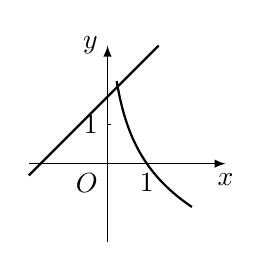
\begin{tikzpicture}[scale = 0.5,>=latex]
    \draw [->] (-2,0) -- (3,0) node [below] {$x$};
    \draw [->] (0,-2) -- (0,3) node [left] {$y$};
    \draw (0,0) node [below left] {$O$};
    \draw (0.1,1) -- (0,1) node [left] {$1$};
    \draw (1,0) node [below] {$1$};
    \draw [thick] (-2,-0.3) -- (1.3,3);
    \draw [thick,domain =-1.1:2.1,samples = 200] plot ({0.5^\x},\x);
\end{tikzpicture}
}{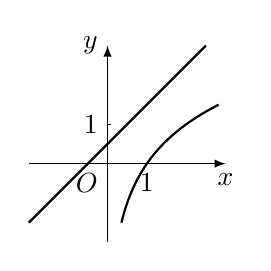
\begin{tikzpicture}[scale = 0.5,>=latex]
    \draw [->] (-2,0) -- (3,0) node [below] {$x$};
    \draw [->] (0,-2) -- (0,3) node [left] {$y$};
    \draw (0,0) node [below left] {$O$};
    \draw (0.1,1) -- (0,1) node [left] {$1$};
    \draw (1,0) node [below] {$1$};
    \draw [thick] (-2,-1.5) -- (2.5,3);
    \draw [thick,domain =1.5:-1.5,samples = 200] plot ({0.5^\x},-\x);
\end{tikzpicture}
}{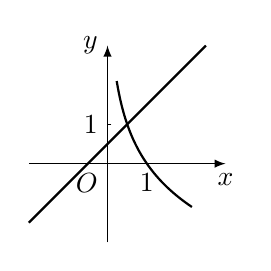
\begin{tikzpicture}[scale = 0.5,>=latex]
    \draw [->] (-2,0) -- (3,0) node [below] {$x$};
    \draw [->] (0,-2) -- (0,3) node [left] {$y$};
    \draw (0,0) node [below left] {$O$};
    \draw (0.1,1) -- (0,1) node [left] {$1$};
    \draw (1,0) node [below] {$1$};
    \draw [thick] (-2,-1.5) -- (2.5,3);
    \draw [thick,domain =-1.1:2.1,samples = 200] plot ({0.5^\x},\x);
\end{tikzpicture}
}{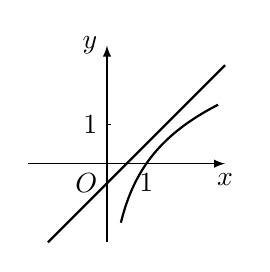
\begin{tikzpicture}[scale = 0.5,>=latex]
    \draw [->] (-2,0) -- (3,0) node [below] {$x$};
    \draw [->] (0,-2) -- (0,3) node [left] {$y$};
    \draw (0,0) node [below left] {$O$};
    \draw (0.1,1) -- (0,1) node [left] {$1$};
    \draw (1,0) node [below] {$1$};
    \draw [thick] (-1.5,-2) -- (3,2.5);
    \draw [thick,domain =1.5:-1.5,samples = 200] plot ({0.5^\x},-\x);
\end{tikzpicture}
}


关联目标:

K0211001B|D02002B|会利用指数函数的单调性解决相关不等式等问题.

K0213007B|D02002B|会作出对数函数的大致图像, 能根据其图像特征叙述函数性质.



标签: 第二单元

答案: 暂无答案

解答或提示: 暂无解答与提示

使用记录:

暂无使用记录


出处: 教材复习题
\item { (000063)}求下列函数的的定义域:\\
(1) $y=(x-1)^{\frac 52}$;\\
(2) $y=3^{\sqrt{x-1}}$;\\
(3) $y=\lg \dfrac{1+x}{1-x}$.


关联目标:

K0207002B|D02002B|会根据具体的幂指数$a$求解幂函数$y=x^{a}$的定义域.

K0209002B|D02002B|会求解有关指数型函数的定义域.

K0212002B|D02002B|会求解有关对数型函数的定义域.



标签: 第二单元

答案: 暂无答案

解答或提示: 暂无解答与提示

使用记录:

暂无使用记录


出处: 教材复习题
\item { (000064)}比较下列各题中两个数的大小:\\
(1) $0.1^{0.7}$与$0.2^{0.7}$;\\
(2) $0.7^{0.1}$与$0.7^{0.2}$;\\
(3) $\log_{0.7}0.1$与$\log_{0.7}0.2$.


关联目标:

K0210006B|D02002B|会利用指数函数的单调性判断两个数的大小.

K0208004B|D02002B|会用幂函数的单调性判断两个幂的大小.

K0213008B|D02002B|会利用对数函数的单调性判断两个数的大小.



标签: 第二单元

答案: 暂无答案

解答或提示: 暂无解答与提示

使用记录:

暂无使用记录


出处: 教材复习题
\item { (000065)}设点$(\sqrt 2, 2)$在幂函数$y_1=x^a$的图像上, 点$(-2,\dfrac 14)$在幂函数$y_2=x^b$的图像上. 当$x$取何值时, $y_1=y_2$?


关联目标:

K0207001B|D02002B|理解幂函数的定义(包含幂函数定义域的概念).



标签: 第二单元

答案: 暂无答案

解答或提示: 暂无解答与提示

使用记录:

暂无使用记录


出处: 教材复习题
\item { (000066)}设$a=(\dfrac 23)^x$, $b=x^{\frac 32}$及$c=\log_\frac{2}{3}x$, 当$x>1$时, 试比较$a$、$b$及$c$之间的大小关系.


关联目标:

K0210006B|D02002B|会利用指数函数的单调性判断两个数的大小.

K0208004B|D02002B|会用幂函数的单调性判断两个幂的大小.

K0213008B|D02002B|会利用对数函数的单调性判断两个数的大小.



标签: 第二单元

答案: 暂无答案

解答或提示: 暂无解答与提示

使用记录:

暂无使用记录


出处: 教材复习题
\item { (000067)}设常数$a>0$且$a\ne 1$, 若函数$y=\log_a(x+1)$在区间$[0, 1]$上的最大值为$1$, 最小值为$0$, 求实数$a$的值.


关联目标:

K0214002B|D02002B|会利用对数函数的单调性解决其他相关不等式等数学问题和生活中的实际问题.



标签: 第二单元

答案: 暂无答案

解答或提示: 暂无解答与提示

使用记录:

暂无使用记录


出处: 教材复习题
\item { (000069)}填空题:\\
(1) 已知$m\in \mathbf{Z}$, 设幂函数$y=x^{m^2-4m}$的图像关于原点成中心对称, 且与$x$轴及$y$轴均无交点, 则$m$的值为\blank{50}.\\
(2) 设$a$、$b$为常数, 若$0<a<1$, $b<-1$, 则函数$y=a^x+b$的图像必定不经过第\blank{50}象限.


关联目标:

K0207004B|D02002B|会用图像上任意一点关于原点(或关于$y$轴)的对称点仍落在图像上证明函数的图像关于原点(或$y$轴)对称.

K0210002B|D02002B|知道指数函数图像过定点$(0,1)$.



标签: 第二单元

答案: 暂无答案

解答或提示: 暂无解答与提示

使用记录:

暂无使用记录


出处: 教材复习题
\item { (000070)}选择题:\\
(1) 若$m>n>1$, 而$0<x<1$, 则下列不等式正确的是\bracket{20}.
\fourch{$m^x<n^x$}{$x^m<x^n$}{$\log_x m>\log_x n$}{$\log_m x<\log_n x$}
(2) 在同一平面直角坐标系中, 二次函数$y=ax^2+bx$与指数函数$y=(\dfrac ba)^x$的图像关系可能为\bracket{20}.
\fourch{
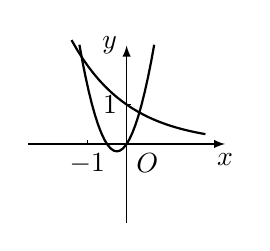
\begin{tikzpicture}[scale = 0.5, >=latex]
    \draw [->] (-2.5,0) -- (2.5,0) node [below] {$x$};
    \draw [->] (0,-2.) -- (0,2.5) node [left] {$y$};
    \draw (0,0) node [below right] {$O$};
    \draw (-1,0.1) -- (-1,0) node [below] {$-1$};
    \draw (0.1,1) -- (0,1) node [left] {$1$};
    \draw [domain = -1.2:0.7,thick] plot (\x,{3*\x * (\x+0.5)});
    \draw [domain = -1.4:2,thick] plot (\x,{(0.5)^\x}); 
\end{tikzpicture}
}{
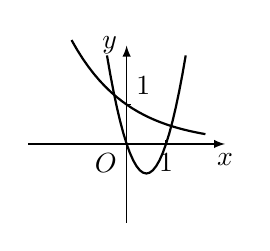
\begin{tikzpicture}[scale = 0.5, >=latex]
    \draw [->] (-2.5,0) -- (2.5,0) node [below] {$x$};
    \draw [->] (0,-2.) -- (0,2.5) node [left] {$y$};
    \draw (0,0) node [below left] {$O$};
    \draw (1,0.1) -- (1,0) node [below] {$1$};
    \draw (0.1,1) -- (0,1) node [above right] {$1$};
    \draw [domain = -0.5:1.5,thick] plot (\x,{3*\x*(\x-1)});
    \draw [domain = -1.4:2,thick] plot (\x,{(0.5)^\x}); 
\end{tikzpicture}
}{
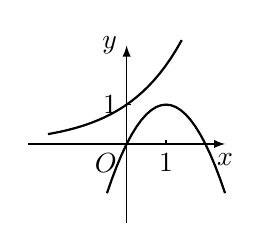
\begin{tikzpicture}[scale = 0.5, >=latex]
    \draw [->] (-2.5,0) -- (2.5,0) node [below] {$x$};
    \draw [->] (0,-2.) -- (0,2.5) node [left] {$y$};
    \draw (0,0) node [below left] {$O$};
    \draw (1,0.1) -- (1,0) node [below] {$1$};
    \draw (0.1,1) -- (0,1) node [left] {$1$};
    \draw [domain = -0.5:2.5,thick] plot ({\x},{-\x*(\x-2)});
    \draw [domain = -1.4:2,thick] plot ({-\x},{(0.5)^\x}); 
\end{tikzpicture}
}{
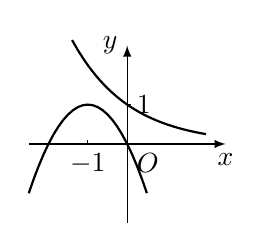
\begin{tikzpicture}[scale = 0.5, >=latex]
    \draw [->] (-2.5,0) -- (2.5,0) node [below] {$x$};
    \draw [->] (0,-2.) -- (0,2.5) node [left] {$y$};
    \draw (0,0) node [below right] {$O$};
    \draw (-1,0.1) -- (-1,0) node [below] {$-1$};
    \draw (0.1,1) -- (0,1) node [right] {$1$};
    \draw [domain = -2.5:0.5,thick] plot ({\x},{-\x*(\x+2)});
    \draw [domain = -1.4:2,thick] plot ({\x},{(0.5)^\x}); 
\end{tikzpicture}   
}


关联目标:

K0208004B|D02002B|会用幂函数的单调性判断两个幂的大小.

K0210006B|D02002B|会利用指数函数的单调性判断两个数的大小.

K0213008B|D02002B|会利用对数函数的单调性判断两个数的大小.

K0210005B|D02002B|会作出指数函数的大致图像, 能根据其图像特征叙述其函数性质.



标签: 第二单元

答案: 暂无答案

解答或提示: 暂无解答与提示

使用记录:

暂无使用记录


出处: 教材复习题
\item { (000071)}设$a$为常数且$0<a<1$, 若$y=(\log_a \dfrac 35)^x$在$\mathbf{R}$上是严格增函数, 求实数$a$的取值范围.


关联目标:

K0211001B|D02002B|会利用指数函数的单调性解决相关不等式等问题.



标签: 第二单元

答案: 暂无答案

解答或提示: 暂无解答与提示

使用记录:

暂无使用记录


出处: 教材复习题
\item { (000072)}在同一平面直角坐标系中, 作出函数$y=(\dfrac 12)^x$及$y=x^{\frac 12}$的大致图像, 并求方程$(\dfrac 12)^x=x^{\frac 12}$的解的个数.


关联目标:

K0207003B|D02002B|会根据函数定义域, 利用计算器合理采点, 并能通过描点法作出幂函数$y=x^{1/2}$,$y=x^{3}$,$y=x^{-2/3}$的大致图像.

K0210005B|D02002B|会作出指数函数的大致图像, 能根据其图像特征叙述其函数性质.



标签: 第二单元

答案: 暂无答案

解答或提示: 暂无解答与提示

使用记录:

暂无使用记录


出处: 教材复习题
\item { (000073)}已知集合$A=\{y|y=(\dfrac 12)^x,\  x\in [-2, 0)\}$, 用列举法表示集合$B=\{y|y=\log_3x,\  x\in A\text{且}y\in \mathbf{Z}\}$.


关联目标:

K0102001B|D01001B|能在具体情境中用列举法描述集合.

K0102002B|D01001B|能在具体情境中用描述法描述集合.

K0210005B|D02002B|会作出指数函数的大致图像, 能根据其图像特征叙述其函数性质.

K0213007B|D02002B|会作出对数函数的大致图像, 能根据其图像特征叙述函数性质.



标签: 第二单元

答案: 暂无答案

解答或提示: 暂无解答与提示

使用记录:

暂无使用记录


出处: 教材复习题
\item { (000074)}$\log_23$是有理数吗? 请证明你的结论.


关联目标:

K0204004B|D02001B|会进行指数式与对数式的互化, 以及对数式的化简.

K0107003B|D01002B|了解反证法的思想以及表达方式, 能正确使用反证法证明一些简单的数学命题.



标签: 第二单元

答案: 暂无答案

解答或提示: 暂无解答与提示

使用记录:

暂无使用记录


出处: 教材复习题
\item { (000075)}仅利用对数函数的单调性和计算器上的乘方功能来确定对数$\log_23$第二位小数的值.


关联目标:

K0214001B|D02002B|会利用对数函数的单调性估算对数型无理数(如$\log_23$).



标签: 第二单元

答案: 暂无答案

解答或提示: 暂无解答与提示

使用记录:

暂无使用记录


出处: 教材复习题
\item { (000330)}若函数$f(x)=\log_2\dfrac{x-a}{x+1}$的反函数的图像过点$(-2,3)$, 则$a=$\blank{50}.


关联目标:

暂未关联目标



标签: 第二单元

答案: $2$

解答或提示: 暂无解答与提示

使用记录:

20211119	2022届高三1班	\fcolorbox[rgb]{0,0,0}{1.000,0.094,0}{0.953}


出处: 赋能练习
\item { (000342)}若函数$f(x)=\begin{cases}    2^x, & x\le 0, \\ -x^2+m, & x>0 \end{cases}$的值域为$(-\infty ,1]$, 则实数$m$的取值范围是\blank{50}.


关联目标:

暂未关联目标



标签: 第二单元

答案: $0<m\le 1$

解答或提示: 暂无解答与提示

使用记录:

20211126	2022届高三1班	\fcolorbox[rgb]{0,0,0}{0.976,1.000,0}{0.488}

20220622	2022届高三1班  	\fcolorbox[rgb]{0,0,0}{1.000,0.140,0}{0.930}


出处: 赋能练习
\item { (000344)}定义在$\mathbf{R}$上的偶函数$y=f(x)$, 当$x\ge 0$时, $f(x)=\lg (x^2-3x+3)$, 则$f(x)$在$\mathbf{R}$上的零点个数为\blank{50}个.


关联目标:

暂未关联目标



标签: 第二单元

答案: $4$

解答或提示: 暂无解答与提示

使用记录:

20211126	2022届高三1班	\fcolorbox[rgb]{0,0,0}{1.000,0.046,0}{0.977}


出处: 赋能练习
\item { (000349)}若函数$f(x)=\log_2 (x+1)+a$的反函数的图像经过点$(4,1)$, 则实数$a=$\blank{50}.


关联目标:

暂未关联目标



标签: 第二单元

答案: $3$

解答或提示: 暂无解答与提示

使用记录:

20211203	2022届高三1班	\fcolorbox[rgb]{0,0,0}{1.000,0.000,0}{1.000}


出处: 赋能练习
\item { (000358)}函数$f(x)=1+\log_2 x$($x\ge 1$)的反函数$f^{-1}(x)=$\blank{50}.


关联目标:

暂未关联目标



标签: 第二单元

答案: $2^{x-1}\ (x\ge 1)$

解答或提示: 暂无解答与提示

使用记录:

20211210	2022届高三1班	\fcolorbox[rgb]{0,0,0}{1.000,0.046,0}{0.977}


出处: 赋能练习
\item { (000362)}方程$\log_2(9^x-5)=2+\log_2(3^x-2)$的解$x=$\blank{50}.


关联目标:

暂未关联目标



标签: 第二单元

答案: $x=1$

解答或提示: 暂无解答与提示

使用记录:

20211210	2022届高三1班	\fcolorbox[rgb]{0,0,0}{1.000,0.136,0}{0.932}


出处: 赋能练习
\item { (000367)}设函数$f(x)=\begin{cases}\log_2 x, & x>0, \\ 4^x, & x\le 0,\end{cases}$ 则$f(f(-1))=$\blank{50}.


关联目标:

暂未关联目标



标签: 第二单元

答案: $-2$

解答或提示: 暂无解答与提示

使用记录:

20211217	2022届高三1班	\fcolorbox[rgb]{0,0,0}{1.000,0.000,0}{1.000}


出处: 赋能练习
\item { (000381)}若点$(8,4)$在函数$f(x)=1+\log_a x$图像上, 则$f(x)$的反函数为\blank{50}.


关联目标:

暂未关联目标



标签: 第二单元

答案: $2^{x-1}$

解答或提示: 暂无解答与提示

使用记录:

20211223	2022届高三1班	\fcolorbox[rgb]{0,0,0}{1.000,0.090,0}{0.955}


出处: 赋能练习
\item { (000388)}已知函数$f(x)=a^x-1$的图像经过$(1,1)$点, 则$f^{-1}(3)=$\blank{50}.


关联目标:

暂未关联目标



标签: 第二单元

答案: $2$

解答或提示: 暂无解答与提示

使用记录:

20211230	2022届高三1班	\fcolorbox[rgb]{0,0,0}{1.000,0.000,0}{1.000}


出处: 赋能练习
\item { (000406)}方程$\lg (3x+4)=1$的解$x=$\blank{50}.


关联目标:

暂未关联目标



标签: 第二单元

答案: $2$

解答或提示: 暂无解答与提示

使用记录:

20220105	2022届高三1班	\fcolorbox[rgb]{0,0,0}{1.000,0.052,0}{0.974}


出处: 赋能练习
\item { (000425)}若关于$x$的不等式$|2^x-m|-\dfrac1{2^x}<0$在区间$[0,1]$内恒成立, 则实数$m$的范围\blank{50}.


关联目标:

暂未关联目标



标签: 第二单元

答案: $(\frac 32,2)$

解答或提示: 暂无解答与提示

使用记录:

20220106	2022届高三1班	\fcolorbox[rgb]{0,0,0}{1.000,0.196,0}{0.902}


出处: 赋能练习
\item { (000450)}函数$f(x)=2^x+m$的反函数为$y=f^{-1}(x)$, 且$y=f^{-1}(x)$的图像过点$Q(5,2)$, 那么$m=$\blank{50}.


关联目标:

暂未关联目标



标签: 第二单元

答案: $1$

解答或提示: 暂无解答与提示

使用记录:

20220221	2022届高三1班	\fcolorbox[rgb]{0,0,0}{1.000,0.000,0}{1.000}


出处: 赋能练习
\item { (000472)}若函数$f(x)=x^a$的反函数的图像经过点$(\dfrac12,\dfrac14)$, 则$a=$\blank{50}.


关联目标:

暂未关联目标



标签: 第二单元

答案: $\frac 12$

解答或提示: 暂无解答与提示

使用记录:

20220223	2022届高三1班	\fcolorbox[rgb]{0,0,0}{1.000,0.140,0}{0.930}


出处: 赋能练习
\item { (000474)}已知函数$y=f(x)$是奇函数, 当$x<0$时, $f(x)=2^x-ax$, 且$f(2)=2$, 则$a=$\blank{50}.


关联目标:

暂未关联目标



标签: 第二单元

答案: $-\frac 98$

解答或提示: 暂无解答与提示

使用记录:

20220223	2022届高三1班	\fcolorbox[rgb]{0,0,0}{1.000,0.186,0}{0.907}


出处: 赋能练习
\item { (000486)}函数$f(x)=\lg(2-x)$的定义域是\blank{50}.


关联目标:

暂未关联目标



标签: 第二单元

答案: $(-\infty ,2)$

解答或提示: 暂无解答与提示

使用记录:

20220225	2022届高三1班	\fcolorbox[rgb]{0,0,0}{1.000,0.000,0}{1.000}


出处: 赋能练习
\item { (000495)}已知函数$f(x)=\begin{cases} 2^x, & x\le 0, \\ f(x-2), & x>0, \end{cases}$ 则$f(1)+f(2)+f(3)+\cdots+f(2017)=$\blank{50}.


关联目标:

暂未关联目标



标签: 第二单元

答案: $\frac{3025}2$

解答或提示: 暂无解答与提示

使用记录:

20220225	2022届高三1班	\fcolorbox[rgb]{0,0,0}{1.000,0.094,0}{0.953}


出处: 赋能练习
\item { (000498)}已知幂函数的图像过点$(2,\dfrac14)$, 则该幂函数的单调递增区间是\blank{50}.


关联目标:

暂未关联目标



标签: 第二单元

答案: $(-\infty ,0)$

解答或提示: 暂无解答与提示

使用记录:

20220228	2022届高三1班	\fcolorbox[rgb]{0,0,0}{1.000,0.190,0}{0.905}


出处: 赋能练习
\item { (000520)}已知函数$f(x)=a\cdot 2^x+3-a\ (a\in \mathbf{R})$的反函数为$y=f^{-1}(x)$, 则函数$y=f^{-1}(x)$的图像经过的定点的坐标为\blank{50}.


关联目标:

暂未关联目标



标签: 第二单元

答案: $(3,0)$

解答或提示: 暂无解答与提示

使用记录:

20220303	2022届高三1班	\fcolorbox[rgb]{0,0,0}{1.000,0.046,0}{0.977}


出处: 赋能练习
\item { (000525)}已知函数$f(x)=\begin{cases} (5-a)x+1, & x<1, \\ a^x, & x\ge 1\end{cases} \ (a>0,a\ne 1)$是实数集$\mathbf{R}$上的增函数, 则实数$a$的取值范围为\blank{50}.


关联目标:

暂未关联目标



标签: 第二单元

答案: $[3,5)$

解答或提示: 暂无解答与提示

使用记录:

20220303	2022届高三1班	\fcolorbox[rgb]{0,0,0}{1.000,0.326,0}{0.837}


出处: 赋能练习
\item { (000538)}方程$\log_2(2-x)+\log_2(3-x)=\log_2 12$的解$x=$\blank{50}.


关联目标:

暂未关联目标



标签: 第二单元

答案: $-1$

解答或提示: 暂无解答与提示

使用记录:

20220307	2022届高三1班	\fcolorbox[rgb]{0,0,0}{1.000,0.000,0}{1.000}


出处: 赋能练习
\item { (000549)}已知函数$f(x)=\log_2(x+a)$的反函数为$y=f^{-1}(x)$, 且$f^{-1}(2)=1$, 则实数$a=$\blank{50}.


关联目标:

暂未关联目标



标签: 第二单元

答案: $3$

解答或提示: 暂无解答与提示

使用记录:

20220309	2022届高三1班	\fcolorbox[rgb]{0,0,0}{1.000,0.090,0}{0.955}


出处: 赋能练习
\item { (000565)}已知函数$f(x)=\begin{cases} \log_2 (x+a), & x\le 0, \\ x^2-3ax+a, & x>0 \end{cases}$有三个不同的零点, 则实数$a$的取值范围是\blank{50}.


关联目标:

暂未关联目标



标签: 第二单元

答案: $a\ge 1$

解答或提示: 暂无解答与提示

使用记录:

20220310	2022届高三1班	\fcolorbox[rgb]{0,0,0}{1.000,0.182,0}{0.909}


出处: 赋能练习
\item { (000567)}函数$f(x)=\sqrt{1-\lg x}$的定义域为\blank{50}.


关联目标:

暂未关联目标



标签: 第二单元

答案: $(0,10 ]$

解答或提示: 暂无解答与提示

使用记录:

20220315	2022届高三1班	\fcolorbox[rgb]{0,0,0}{1.000,0.094,0}{0.953}


出处: 赋能练习
\item { (000582)}数列$\{a_n\}$的前$n$项和为$S_n$, 若点$(n,S_n) \ (n\in \mathbf{N}^*)$在函数$y=\log_2 (x+1)$的反函数的图像上, 则$a_n$=\blank{50}.


关联目标:

暂未关联目标



标签: 第二单元

答案: $a_n=2^{n-1}$

解答或提示: 暂无解答与提示

使用记录:

20220316	2022届高三1班	\fcolorbox[rgb]{0,0,0}{1.000,0.326,0}{0.837}


出处: 赋能练习
\item { (000590)}已知函数$f(x)=1+\log_a x$, $y=f^{-1}(x)$是函数$y=f(x)$的反函数, 若$y=f^{-1}(x)$的图像过点$(2,4)$, 则$a$的值为\blank{50}.


关联目标:

暂未关联目标



标签: 第二单元

答案: $4$

解答或提示: 暂无解答与提示

使用记录:

20220322	2022届高三1班	\fcolorbox[rgb]{0,0,0}{1.000,0.000,0}{1.000}


出处: 赋能练习
\item { (000594)}已知函数$f(x)$是定义在$\mathbf{R}$上且周期为$4$的偶函数. 当$x\in [2,4]$时, $f(x)=\left|\log_4(x-\dfrac32)\right|$, 则$f(\dfrac12)$的值为\blank{50}.


关联目标:

暂未关联目标



标签: 第二单元

答案: $\dfrac 12$

解答或提示: 暂无解答与提示

使用记录:

20220322	2022届高三1班	\fcolorbox[rgb]{0,0,0}{1.000,0.094,0}{0.953}


出处: 赋能练习
\item { (000604)}已知函数$f(x)=\begin{cases} \log_2 x, & 0<x<2, \\ (\dfrac23)^x+\dfrac59, & x\ge 2. \end{cases}$ 若函数$g(x)=f(x)-k$有两个不同的零点, 则实数$k$的取值范围是\blank{50}.


关联目标:

暂未关联目标



标签: 第二单元

答案: $(\frac 59,1)$

解答或提示: 暂无解答与提示

使用记录:

20220323	2022届高三1班	\fcolorbox[rgb]{0,0,0}{1.000,0.326,0}{0.837}


出处: 赋能练习
\item { (000607)}函数$y=\log_2(1-\dfrac1x)$的定义域为\blank{50}.


关联目标:

暂未关联目标



标签: 第二单元

答案: $(-\infty ,0)\cup (1,+\infty)$

解答或提示: 暂无解答与提示

使用记录:

20220324	2022届高三1班	\fcolorbox[rgb]{0,0,0}{1.000,0.140,0}{0.930}


出处: 赋能练习
\item { (000614)}若函数$f(x)=\log_2^2x-\log_2 x+1 \ (x\ge 2)$的反函数为$f^{-1}(x)$, 则$f^{-1}(3)$=\blank{50}.


关联目标:

暂未关联目标



标签: 第二单元

答案: $4$

解答或提示: 暂无解答与提示

使用记录:

20220324	2022届高三1班	\fcolorbox[rgb]{0,0,0}{1.000,0.094,0}{0.953}


出处: 赋能练习
\item { (000616)}方程$\log_3(2x+1)=2$的解是\blank{50}.


关联目标:

暂未关联目标



标签: 第二单元

答案: $x=4$

解答或提示: 暂无解答与提示

使用记录:

20220325	2022届高三1班	\fcolorbox[rgb]{0,0,0}{1.000,0.000,0}{1.000}


出处: 赋能练习
\item { (000622)}若函数$f(x)=2^x(x+a)-1$在区间$[0,1]$上有零点, 则实数$a$的取值范围是\blank{50}.


关联目标:

暂未关联目标



标签: 第二单元

答案: $[-\frac 12,1]$

解答或提示: 暂无解答与提示

使用记录:

20220325	2022届高三1班	\fcolorbox[rgb]{0,0,0}{1.000,0.280,0}{0.860}


出处: 赋能练习
\item { (000634)}若函数$f(x)=4^x+2^{x+1}$的图像与函数$y=g(x)$的图像关于直线$y=x$对称, 则$g(3)=$\blank{50}.


关联目标:

暂未关联目标



标签: 第二单元|第七单元

答案: $0$

解答或提示: 暂无解答与提示

使用记录:

20220329	2022届高三1班	\fcolorbox[rgb]{0,0,0}{1.000,0.046,0}{0.977}


出处: 赋能练习
\item { (000650)}若函数$f(x)=\begin{cases} -x+3a, & x<0,  \\ a^x+1, & x\ge 0 \end{cases}$($a>0$, 且$a\ne 1$)是$\mathbf{R}$上的减函数, 则$a$的取值范围是\blank{50}.


关联目标:

暂未关联目标



标签: 第二单元

答案: $[\frac 23,1)$

解答或提示: 暂无解答与提示

使用记录:

20220401	2022届高三1班	\fcolorbox[rgb]{0,0,0}{1.000,0.048,0}{0.976}


出处: 赋能练习
\item { (000656)}已知集合$A=\{x|\ln x>0 \}$, $B=\{x|2^x<3\}$, 则\blank{50}.


关联目标:

暂未关联目标



标签: 第二单元

答案: $(1,\log_2 3)$

解答或提示: 暂无解答与提示

使用记录:

20220406	2022届高三1班	\fcolorbox[rgb]{0,0,0}{1.000,0.094,0}{0.953}


出处: 赋能练习
\item { (000660)}设$f(x)$为$\mathbf{R}$上的奇函数. 当$x\ge 0$时, $f(x)=2^x+2x+b$($b$为常数), 则$f(-1)$的值为\blank{50}.


关联目标:

暂未关联目标



标签: 第二单元

答案: $-3$

解答或提示: 暂无解答与提示

使用记录:

20220406	2022届高三1班	\fcolorbox[rgb]{0,0,0}{1.000,0.140,0}{0.930}


出处: 赋能练习
\item { (000675)}已知定义在$\mathbf{R}$上的函数$f(x)$满足: \textcircled{1} $f(x)+f(2-x)=0$; \textcircled{2} $f(x)-f(-2-x)=0$; \textcircled{3} 在$[-1,1]$上的表达式为$f(x)=\begin{cases} \sqrt{1-x^2}, & x\in [-1,0], \\ 1-x, & x\in (0,1] \end{cases}$, 则函数$f(x)$与函数$g(x)=\begin{cases} 2^x, & x\le 0, \\ \log_{\frac12} x,& x>0 \end{cases}$的图像在区间$[-3,3]$上的交点的个数为\blank{50}.


关联目标:

暂未关联目标



标签: 第二单元

答案: $6$

解答或提示: 暂无解答与提示

使用记录:

20220408	2022届高三1班	\fcolorbox[rgb]{0,0,0}{1.000,0.418,0}{0.791}


出处: 赋能练习
\item { (000693)}已知函数$f(x)=\begin{cases}2^x, & x\le 0, \\ \log_2 x, & 0<x\le 1\end{cases}$的反函数是$f^{-1}(x)$, 则$f^{-1}(\dfrac12)=$\blank{50}.


关联目标:

暂未关联目标



标签: 第二单元

答案: $-1$

解答或提示: 暂无解答与提示

使用记录:

20220419	2022届高三1班	\fcolorbox[rgb]{0,0,0}{1.000,0.046,0}{0.977}


出处: 赋能练习
\item { (000702)}设$f(x)$是定义在$\mathbf{R}$上的奇函数, 当$x>0$时,$f(x)=2^x-3$. 则不等式$f(x)<-5$的解为\blank{50}.


关联目标:

暂未关联目标



标签: 第二单元

答案: $(-\infty,-3)$

解答或提示: 暂无解答与提示

使用记录:

20220420	2022届高三1班	\fcolorbox[rgb]{0,0,0}{1.000,0.140,0}{0.930}


出处: 赋能练习
\item { (000724)}设$f(x)$是定义在$\mathbf{R}$上以$2$为周期的偶函数, 当$x\in [0,1]$时, $f(x)=\log_2(x+1)$, 则函数$f(x)$在$[1,2]$上的解析式是\blank{50}.


关联目标:

暂未关联目标



标签: 第二单元

答案: $f(x)=\log_2(3-x)$

解答或提示: 暂无解答与提示

使用记录:

20220424	2022届高三1班	\fcolorbox[rgb]{0,0,0}{1.000,0.046,0}{0.977}


出处: 赋能练习
\item { (000734)}给出下列函数: \textcircled{1} $y=x+\dfrac1x$; \textcircled{2} $y={x^2}+x$; \textcircled{3} $y={2^{|x|}}$; \textcircled{4} $y={x^{\dfrac23}}$; \textcircled{5} $y=\tan x$; \textcircled{6} $y=\sin(\arccos x)$; \textcircled{7} $y=\lg(x+\sqrt{{x^2}+4})-\lg 2$. 从这$7$个函数中任取两个函数, 则其中一个是奇函数另一个是偶函数的概率是\blank{50}.


关联目标:

暂未关联目标



标签: 第二单元

答案: $\frac 37$

解答或提示: 暂无解答与提示

使用记录:

20220426	2022届高三1班	\fcolorbox[rgb]{0,0,0}{1.000,0.466,0}{0.767}


出处: 赋能练习
\item { (000738)}函数$f(x)=\lg (3^x-2^x)$的定义域为\blank{50}.


关联目标:

暂未关联目标



标签: 第二单元

答案: $(0,+\infty)$

解答或提示: 暂无解答与提示

使用记录:

20220427	2022届高三1班	\fcolorbox[rgb]{0,0,0}{1.000,0.280,0}{0.860}


出处: 赋能练习
\item { (000761)}方程$\log_3(3 \cdot 2^x+5)-\log_3(4^x+1)=0$的解$x=$\blank{50}.


关联目标:

暂未关联目标



标签: 第二单元

答案: $2$

解答或提示: 暂无解答与提示

使用记录:

20220506	2022届高三1班	\fcolorbox[rgb]{0,0,0}{1.000,0.000,0}{1.000}


出处: 赋能练习
\item { (000767)}函数$y=\lg x$的反函数是\blank{50}.


关联目标:

暂未关联目标



标签: 第二单元

答案: $y=10^x$

解答或提示: 暂无解答与提示

使用记录:

20220507	2022届高三1班	\fcolorbox[rgb]{0,0,0}{1.000,0.000,0}{1.000}


出处: 赋能练习
\item { (000778)}函数$y=\sqrt{\lg(x+2)}$的定义域为\blank{50}.


关联目标:

暂未关联目标



标签: 第二单元

答案: $\{x|x\ge -1\}$

解答或提示: 暂无解答与提示

使用记录:

20220510	2022届高三1班	\fcolorbox[rgb]{0,0,0}{1.000,0.046,0}{0.977}


出处: 赋能练习
\item { (000789)}定义在$\mathbf{R}$上的函数$f(x)=2^x-1$的反函数为$y=f^{-1}(x)$, 则$f^{-1}(3)=$\blank{50}.


关联目标:

暂未关联目标



标签: 第二单元

答案: $2$

解答或提示: 暂无解答与提示

使用记录:

20220511	2022届高三1班	\fcolorbox[rgb]{0,0,0}{1.000,0.000,0}{1.000}


出处: 赋能练习
\item { (000795)}若函数$f(x)={\log_a}(x^2-ax+1)\ (a>0, \ a\ne 1)$没有最小值, 则$a$的取值范围是\blank{50}.


关联目标:

暂未关联目标



标签: 第二单元

答案: $(0,1)\cup [2,+\infty)$

解答或提示: 暂无解答与提示

使用记录:

20220511	2022届高三1班	\fcolorbox[rgb]{0,0,0}{1.000,0.512,0}{0.744}

20220622	2022届高三1班  	\fcolorbox[rgb]{0,0,0}{1.000,0.232,0}{0.884}


出处: 赋能练习
\item { (000799)}已知$f^{-1}(x)$是函数$f(x)=\log_2(x+1)$的反函数, 则$f^{-1}(2)=$\blank{50}.


关联目标:

暂未关联目标



标签: 第二单元

答案: $3$

解答或提示: 暂无解答与提示

使用记录:

20220513	2022届高三1班	\fcolorbox[rgb]{0,0,0}{1.000,0.046,0}{0.977}


出处: 赋能练习
\item { (000824)}已知$f(x)$是定义在$[-2,2]$上的奇函数, 当$x\in (0,2]$时,$f(x)=2^x-1$, 函数$g(x)=x^2-2x+m$. 如果对于任意的$x_1\in [-2,2]$, 总存在$x_2\in [-2,2]$, 使得$f(x_1)\le g(x_2)$, 则实数$m$的取值范围是\blank{50}.


关联目标:

暂未关联目标



标签: 第二单元

答案: $m\ge -5$

解答或提示: 暂无解答与提示

使用记录:

20220519	2022届高三1班	\fcolorbox[rgb]{0,0,0}{1.000,0.418,0}{0.791}


出处: 赋能练习
\item { (000826)}函数$y=\lg x-1$的零点是\blank{50}.


关联目标:

暂未关联目标



标签: 第二单元

答案: $x=10$

解答或提示: 暂无解答与提示

使用记录:

20220520	2022届高三1班	\fcolorbox[rgb]{0,0,0}{1.000,0.000,0}{1.000}


出处: 赋能练习
\item { (000845)}已知函数$f(x)=\lg (\sqrt{x^2+1}+ax)$的定义域为$\mathbf{R}$, 则实数$a$的取值范围是\blank{50}.


关联目标:

暂未关联目标



标签: 第二单元

答案: $[-1, 1]$

解答或提示: 暂无解答与提示

使用记录:

20220525	2022届高三1班	\fcolorbox[rgb]{0,0,0}{1.000,0.094,0}{0.953}


出处: 赋能练习
\item { (000850)}方程$\log_2(9^x+7)=2+\log_2(3^x+1)$的解为\blank{50}.


关联目标:

暂未关联目标



标签: 第二单元

答案: $\{0,1\}$

解答或提示: 暂无解答与提示

使用记录:

20220526	2022届高三1班	\fcolorbox[rgb]{0,0,0}{1.000,0.000,0}{1.000}


出处: 赋能练习
\item { (000863)}设定义在$\mathbf{R}$上的奇函数$y=f(x)$, 当$x>0$时, $f(x)=2^x-4$, 则不等式$f(x)\le 0$的解集是\blank{50}.


关联目标:

暂未关联目标



标签: 第二单元

答案: $(-\infty, -2]\cup [0,2]$

解答或提示: 暂无解答与提示

使用记录:

20220527	2022届高三1班	\fcolorbox[rgb]{0,0,0}{1.000,0.326,0}{0.837}


出处: 赋能练习
\item { (000890)}设函数$f(x)=a^x+a^{-x}  \ (a>0, \ a\ne 1)$, 且$f(1)=3$, 则$f(0)+f(1)+f(2)$的值是\blank{50}.


关联目标:

暂未关联目标



标签: 第二单元

答案: $12$

解答或提示: 暂无解答与提示

使用记录:

20220607	2022届高三1班	\fcolorbox[rgb]{0,0,0}{1.000,0.000,0}{1.000}


出处: 赋能练习
\item { (000918)}若函数$f(x)=\log _5 x$($x>0$), 则方程$f(x+1)+f(x-3)=1$的解$x=$\blank{50}.


关联目标:

暂未关联目标



标签: 第二单元

答案: $4$.

解答或提示: 暂无解答与提示

使用记录:

20220615	2022届高三1班	\fcolorbox[rgb]{0,0,0}{1.000,0.000,0}{1.000}


出处: 赋能练习
\item { (000926)}已知函数$f(x)=\begin{cases}2^x +a, & x\ge 0, \\ x^2-ax, & x<0.\end{cases}$ 若$f(x)$的最小值是$a$, 则$a=$\blank{50}.


关联目标:

暂未关联目标



标签: 第二单元

答案: $-4$

解答或提示: 暂无解答与提示

使用记录:

20220621	2022届高三1班	\fcolorbox[rgb]{0,0,0}{1.000,0.000,0}{1.000}


出处: 赋能练习
\item { (000931)}函数$y=\log_3 (x-1)$的定义域是\blank{50}.


关联目标:

暂未关联目标



标签: 第二单元

答案: $(1,+\infty)$

解答或提示: 暂无解答与提示

使用记录:

20220622	2022届高三1班	\fcolorbox[rgb]{0,0,0}{1.000,0.000,0}{1.000}


出处: 赋能练习
\item { (000949)}已知函数$f(x)={x^3}+\lg (\sqrt{x^2+1}+x)$, 若$f(x)$的定义域中的$a$、$b$满足$f(-a)+f(-b)-3=f(a)+f(b)+3$, 则$f(a)+f(b)=$\blank{50}.


关联目标:

暂未关联目标



标签: 第二单元

答案: $-3$

解答或提示: 暂无解答与提示

使用记录:

20220624	2022届高三1班	\fcolorbox[rgb]{0,0,0}{1.000,0.046,0}{0.977}


出处: 赋能练习
\item { (000954)}函数$y=\sqrt{2^x-1}$的定义域是\blank{50}(用区间表示).


关联目标:

暂未关联目标



标签: 第二单元

答案: $[0,+\infty)$

解答或提示: 暂无解答与提示

使用记录:

20220628	2022届高三1班	\fcolorbox[rgb]{0,0,0}{1.000,0.000,0}{1.000}


出处: 赋能练习
\item { (000961)}已知函数$f(x)=2^x-a\cdot 2^{-x}$的反函数是$f^{-1}(x)$, $f^{-1}(x)$在定义域上是奇函数, 则正实数$a=$\blank{50}.


关联目标:

暂未关联目标



标签: 第二单元

答案: $a=1$

解答或提示: 暂无解答与提示

使用记录:

20220628	2022届高三1班	\fcolorbox[rgb]{0,0,0}{1.000,0.000,0}{1.000}


出处: 赋能练习
\item { (000965)}指数方程$4^x-6 \times 2^x-16=0$的解是\blank{50}.


关联目标:

暂未关联目标



标签: 第二单元

答案: $x=3$

解答或提示: 暂无解答与提示

使用记录:

20220629    2022届高三1班  	\fcolorbox[rgb]{0,0,0}{1.000,0.094,0}{0.953}


出处: 赋能练习
\item { (001161)}下列两个函数是同一个函数的有\blank{50}.\\ 
(1) $y=\dfrac{x^2-1}{x-1}$与$y=x+1$;\\ 
(2) $y=\dfrac{x^3}{x}$与$y=x^2$;\\ 
(3) $y=\sqrt{x^2}-1$与$y=\sqrt[3]{x^3}-1$;\\ 
(4) $f(x)=x^2-2x-1$与$g(t)=t^2-2t-1$;\\ 
(5) $f(x)=2^x, \ x \in \{0,1,2,3\}$与$g(x)=\dfrac16x^3+\dfrac56x+1, \ x \in \{0,1,2,3\}$.


关联目标:

暂未关联目标



标签: 第二单元

答案: 暂无答案

解答或提示: 暂无解答与提示

使用记录:

2016届11班	\fcolorbox[rgb]{0,0,0}{1.000,0.106,0}{0.947}

2016届12班	\fcolorbox[rgb]{0,0,0}{1.000,0.210,0}{0.895}


出处: 2016届创新班作业	1131-函数与函数的三要素
\item { (001192)}写出下列函数的反函数(注意定义域).\\ 
(1) $y=-\dfrac{1}{x}+3$;\\ 
(2) $y=\sqrt{2x-1}$;\\ 
(3) $y=\dfrac{2x+1}{x+2}$;\\ 
(4) $y=x^2+2, \ x\in [2,+\infty)$;\\ 
(5) $y=2^x, \ x\in \{1,2,3,4\}$ (本小题不能使用对数);\\ 
(6) $y=\sqrt{9-x^2}, \ x\in [-3,0]$;\\ 
(7) $y=x^2-4x, x \in [3,7]$.


关联目标:

暂未关联目标



标签: 第二单元

答案: 暂无答案

解答或提示: 暂无解答与提示

使用记录:

2016届11班	\fcolorbox[rgb]{0,0,0}{1.000,0.102,0}{0.949}	\fcolorbox[rgb]{0,0,0}{1.000,0.154,0}{0.923}	\fcolorbox[rgb]{0,0,0}{1.000,0.154,0}{0.923}	\fcolorbox[rgb]{0,0,0}{1.000,0.102,0}{0.949}	\fcolorbox[rgb]{0,0,0}{1.000,0.462,0}{0.769}	\fcolorbox[rgb]{0,0,0}{1.000,0.974,0}{0.513}	\fcolorbox[rgb]{0,0,0}{1.000,0.256,0}{0.872}

2016届12班	\fcolorbox[rgb]{0,0,0}{1.000,0.052,0}{0.974}	\fcolorbox[rgb]{0,0,0}{1.000,0.158,0}{0.921}	\fcolorbox[rgb]{0,0,0}{1.000,0.264,0}{0.868}	\fcolorbox[rgb]{0,0,0}{1.000,0.052,0}{0.974}	\fcolorbox[rgb]{0,0,0}{1.000,0.894,0}{0.553}	\fcolorbox[rgb]{0,0,0}{0.790,1.000,0}{0.395}	\fcolorbox[rgb]{0,0,0}{1.000,0.210,0}{0.895}


出处: 2016届创新班作业	1136-逆映射与反函数
\item { (001209)}已知$a>0$且$a\ne 1$, $f_a(x)=\dfrac{1}{2}+\dfrac{1}{a^x-1},\ x \in \mathbf{Z}^+\cup \mathbf{Z}^-$. 对于每一个$a$分析$f_a(x)$的奇偶性.


关联目标:

暂未关联目标



标签: 第二单元

答案: 暂无答案

解答或提示: 暂无解答与提示

使用记录:

2016届11班	\fcolorbox[rgb]{0,0,0}{0.666,1.000,0}{0.333}

2016届12班	\fcolorbox[rgb]{0,0,0}{0.378,1.000,0}{0.189}


出处: 2016届创新班作业	1138-函数的奇偶性
\item { (001286)}$\dfrac{\sqrt{3\sqrt{3\sqrt{3\sqrt{\dfrac{1}{3}}}}}}{\sqrt{27\sqrt{\dfrac{1}{3}}}}$用$3$的有理数指数幂表示为\blank{80}.


关联目标:

暂未关联目标



标签: 第二单元

答案: 暂无答案

解答或提示: 暂无解答与提示

使用记录:

2016届11班	\fcolorbox[rgb]{0,0,0}{1.000,0.102,0}{0.949}

2016届12班	\fcolorbox[rgb]{0,0,0}{1.000,0.108,0}{0.946}


出处: 2016届创新班作业	1150-有理数指数幂
\item { (001287)}已知$m,n$是有理数, 则以下各说法中, 正确的有\blank{50}.
\vartwoch{对一切$m,n$均成立$2^m2^n=2^{m+n}$}{存在$m,n$使得$2^m2^n=2^{mn}$}{存在$m,n$使得$2^m+2^n=2^{m+n}$}{存在$m,n$使得$(2^m)^n=2^{m^n}$}


关联目标:

暂未关联目标



标签: 第二单元

答案: 暂无答案

解答或提示: 暂无解答与提示

使用记录:

2016届11班	\fcolorbox[rgb]{0,0,0}{1.000,0.154,0}{0.923}

2016届12班	\fcolorbox[rgb]{0,0,0}{1.000,0.216,0}{0.892}


出处: 2016届创新班作业	1150-有理数指数幂
\item { (001292)}已知$a,b$是实数, 函数$f(x)=a\cdot b^x$, 且$f(4)=648$, $f(5)=1944$, 求$f(9/2)$.


关联目标:

暂未关联目标



标签: 第二单元

答案: 暂无答案

解答或提示: 暂无解答与提示

使用记录:

2016届11班	\fcolorbox[rgb]{0,0,0}{1.000,0.052,0}{0.974}

2016届12班	\fcolorbox[rgb]{0,0,0}{1.000,0.054,0}{0.973}


出处: 2016届创新班作业	1151-实数指数幂
\item { (001293)}(1) 求证: 当$a>0$时, $f(x)=\dfrac{a^x-a^{-x}}{2}$是奇函数;\\ 
(2) 求证: 当$a>0$时, $f(x)=x\cdot \dfrac{a^x-1}{a^x+1}$是偶函数.


关联目标:

暂未关联目标



标签: 第二单元

答案: 暂无答案

解答或提示: 暂无解答与提示

使用记录:

2016届11班	\fcolorbox[rgb]{0,0,0}{1.000,0.872,0}{0.564}	\fcolorbox[rgb]{0,0,0}{1.000,0.872,0}{0.564}

2016届12班	\fcolorbox[rgb]{0,0,0}{1.000,0.432,0}{0.784}	\fcolorbox[rgb]{0,0,0}{1.000,0.432,0}{0.784}


出处: 2016届创新班作业	1151-实数指数幂
\item { (001294)}设$a^{2x}=2$, 且$a>0$, $a \ne 1$, 求$\dfrac{a^{3x}+a^{-3x}}{a^x+a^{-x}}$的值.


关联目标:

暂未关联目标



标签: 第二单元

答案: 暂无答案

解答或提示: 暂无解答与提示

使用记录:

2016届11班	\fcolorbox[rgb]{0,0,0}{1.000,0.102,0}{0.949}

2016届12班	\fcolorbox[rgb]{0,0,0}{1.000,0.054,0}{0.973}


出处: 2016届创新班作业	1151-实数指数幂
\item { (001295)}在课堂上我们介绍了等式$\left(\sqrt{2}^{\sqrt{2}}\right)^{\sqrt{2}}=2$, 它的特点是左边是一些无理数指数幂, 而且左边只出现了一个实数, 而且这个实数是无理数; 右边是一个正整数. 你能再写出一个有这样特点的等式吗?


关联目标:

暂未关联目标



标签: 第二单元

答案: 暂无答案

解答或提示: 暂无解答与提示

使用记录:

2016届11班	\fcolorbox[rgb]{0,0,0}{1.000,0.052,0}{0.974}

2016届12班	\fcolorbox[rgb]{0,0,0}{1.000,0.054,0}{0.973}


出处: 2016届创新班作业	1151-实数指数幂
\item { (001296)}求值: $\log_2 0.5=$\blank{80}, $\log_9 27=$\blank{80}, $3^{1+\log_3 5}=$\blank{80}.


关联目标:

暂未关联目标



标签: 第二单元

答案: 暂无答案

解答或提示: 暂无解答与提示

使用记录:

2016届11班	\fcolorbox[rgb]{0,0,0}{1.000,0.052,0}{0.974}

2016届12班	\fcolorbox[rgb]{0,0,0}{1.000,0.054,0}{0.973}


出处: 2016届创新班作业	1152-对数的概念与运算[1]
\item { (001297)}如果$\log_x\sqrt{5}=-1$, 那么$x=$\blank{80}.


关联目标:

暂未关联目标



标签: 第二单元

答案: 暂无答案

解答或提示: 暂无解答与提示

使用记录:

2016届11班	\fcolorbox[rgb]{0,0,0}{1.000,0.000,0}{1.000}

2016届12班	\fcolorbox[rgb]{0,0,0}{1.000,0.000,0}{1.000}


出处: 2016届创新班作业	1152-对数的概念与运算[1]
\item { (001298)}如果$\log_2 y=6$, $\log_x 3=\dfrac{1}{2}$, 那么$x=$\blank{80}, $y=$\blank{80}.


关联目标:

暂未关联目标



标签: 第二单元

答案: 暂无答案

解答或提示: 暂无解答与提示

使用记录:

2016届11班	\fcolorbox[rgb]{0,0,0}{1.000,0.158,0}{0.921}

2016届12班	\fcolorbox[rgb]{0,0,0}{1.000,0.108,0}{0.946}


出处: 2016届创新班作业	1152-对数的概念与运算[1]
\item { (001299)}如果$\log_2(\log_3(\log_4x))=0$, 那么$x=$\blank{80}.


关联目标:

暂未关联目标



标签: 第二单元

答案: 暂无答案

解答或提示: 暂无解答与提示

使用记录:

2016届11班	\fcolorbox[rgb]{0,0,0}{1.000,0.000,0}{1.000}

2016届12班	\fcolorbox[rgb]{0,0,0}{1.000,0.054,0}{0.973}


出处: 2016届创新班作业	1152-对数的概念与运算[1]
\item { (001300)}用不含对数的式子表示:\\ 
(1) 若$\log_7 2=a$, 则$\log_7 14=$\blank{80}, $\log_7 \sqrt{3.5}=$\blank{80}.\\ 
(2) 若$\log_3 2=a$, 则$\log_3 4=$\blank{80}, $\log_3 \dfrac{2}{3}=$\blank{80}.\\ 
(3) 若$\lg 2=a$, 则$\lg 25=$\blank{80}.


关联目标:

暂未关联目标



标签: 第二单元

答案: 暂无答案

解答或提示: 暂无解答与提示

使用记录:

2016届11班	\fcolorbox[rgb]{0,0,0}{1.000,0.052,0}{0.974}	\fcolorbox[rgb]{0,0,0}{1.000,0.052,0}{0.974}	\fcolorbox[rgb]{0,0,0}{1.000,0.106,0}{0.947}

2016届12班	\fcolorbox[rgb]{0,0,0}{1.000,0.108,0}{0.946}	\fcolorbox[rgb]{0,0,0}{1.000,0.054,0}{0.973}	\fcolorbox[rgb]{0,0,0}{1.000,0.108,0}{0.946}


出处: 2016届创新班作业	1152-对数的概念与运算[1]
\item { (001301)}如果$N=923$, 那么$N$的常用对数的首数为\blank{80}.


关联目标:

暂未关联目标



标签: 第二单元

答案: 暂无答案

解答或提示: 暂无解答与提示

使用记录:

2016届11班	\fcolorbox[rgb]{0,0,0}{1.000,0.000,0}{1.000}

2016届12班	\fcolorbox[rgb]{0,0,0}{1.000,0.054,0}{0.973}


出处: 2016届创新班作业	1152-对数的概念与运算[1]
\item { (001302)}如果$N$的常用对数的首数为$1$, 那么$N$的取值范围为\blank{80}.


关联目标:

暂未关联目标



标签: 第二单元

答案: 暂无答案

解答或提示: 暂无解答与提示

使用记录:

2016届11班	\fcolorbox[rgb]{0,0,0}{1.000,0.158,0}{0.921}

2016届12班	\fcolorbox[rgb]{0,0,0}{1.000,0.108,0}{0.946}


出处: 2016届创新班作业	1152-对数的概念与运算[1]
\item { (001303)}如果$N$的常用对数的首数比$M$的常用对数的首数大$3$, 尾数相同, 那么$\dfrac{N}{M}=$\blank{80}.


关联目标:

暂未关联目标



标签: 第二单元

答案: 暂无答案

解答或提示: 暂无解答与提示

使用记录:

2016届11班	\fcolorbox[rgb]{0,0,0}{1.000,0.210,0}{0.895}

2016届12班	\fcolorbox[rgb]{0,0,0}{1.000,0.000,0}{1.000}


出处: 2016届创新班作业	1152-对数的概念与运算[1]
\item { (001304)}$2^{10000}$的常用对数的首数为\blank{80}, $2^{10000}$是\blank{80}位数.


关联目标:

暂未关联目标



标签: 第二单元

答案: 暂无答案

解答或提示: 暂无解答与提示

使用记录:

2016届11班	\fcolorbox[rgb]{0,0,0}{1.000,0.422,0}{0.789}

2016届12班	\fcolorbox[rgb]{0,0,0}{1.000,0.324,0}{0.838}


出处: 2016届创新班作业	1152-对数的概念与运算[1]
\item { (001305)}计算下列各式(要有必要的过程):
\begin{multicols}{2}
(1) $\dfrac{1}{2}\log_{20}45-\log_{20}30$;\\ 
(2) $\dfrac{\lg3+\dfrac{2}{5}\lg9+\dfrac{3}{5}\lg\sqrt{27}-\lg\sqrt{3}}{\lg81-\lg27}$;\\ 
\end{multicols}
\begin{multicols}{2}
(3) $\lg^22+\lg^25+2\lg2\lg5$; \\ 
(4) $\lg^32+\lg^35+3\lg2\lg5$;\hfill\\ 
\end{multicols}
\begin{multicols}{2}
(5) $\lg4+2\sqrt{\lg^26-\lg6^2+1}+\lg9$.\\ 
\end{multicols}


关联目标:

暂未关联目标



标签: 第二单元

答案: 暂无答案

解答或提示: 暂无解答与提示

使用记录:

2016届11班	\fcolorbox[rgb]{0,0,0}{1.000,0.052,0}{0.974}	\fcolorbox[rgb]{0,0,0}{1.000,0.158,0}{0.921}	\fcolorbox[rgb]{0,0,0}{1.000,0.000,0}{1.000}

2016届12班	\fcolorbox[rgb]{0,0,0}{1.000,0.054,0}{0.973}	\fcolorbox[rgb]{0,0,0}{1.000,0.108,0}{0.946}	\fcolorbox[rgb]{0,0,0}{1.000,0.000,0}{1.000}


出处: 2016届创新班作业	1152-对数的概念与运算[1]
\item { (001306)}如果方程$\lg^2x+(\lg2+\lg3)\lg x+\lg2\cdot\lg3=0$的两个根是$x_1,x_2$, 求$x_1x_2$的值.


关联目标:

暂未关联目标



标签: 第二单元

答案: 暂无答案

解答或提示: 暂无解答与提示

使用记录:

2016届11班	\fcolorbox[rgb]{0,0,0}{1.000,0.316,0}{0.842}

2016届12班	\fcolorbox[rgb]{0,0,0}{1.000,0.054,0}{0.973}


出处: 2016届创新班作业	1152-对数的概念与运算[1]
\item { (001307)}已知$a=\log_3 36$, $b=\log_4 36$. 求$\dfrac{2}{a}+\dfrac{1}{b}$.(提示: 你学过实数指数幂的运算律的)


关联目标:

暂未关联目标



标签: 第二单元

答案: 暂无答案

解答或提示: 暂无解答与提示

使用记录:

2016届11班	\fcolorbox[rgb]{0,0,0}{1.000,0.106,0}{0.947}

2016届12班	\fcolorbox[rgb]{0,0,0}{1.000,0.162,0}{0.919}


出处: 2016届创新班作业	1152-对数的概念与运算[1]
\item { (001308)}[证明对数的{\bf 换底公式}]
若$a,b,N>0$, $a\ne 1, b\ne 1$, 则
$$\log_aN=\dfrac{\log_b N}{\log_b a}.$$


关联目标:

暂未关联目标



标签: 第二单元

答案: 暂无答案

解答或提示: 暂无解答与提示

使用记录:

2016届11班	\fcolorbox[rgb]{0,0,0}{1.000,0.106,0}{0.947}

2016届12班	\fcolorbox[rgb]{0,0,0}{1.000,0.000,0}{1.000}


出处: 2016届创新班作业	1152-对数的概念与运算[1]
\item { (001309)}(1) 若$\lg 3=a$, $\lg 2=b$, 则$\log_6 12=$\blank{80}.\\ 
(2) 若$\log_{\sqrt{3}} 2=a$, 则$\log_{12} 3=$\blank{80}.


关联目标:

暂未关联目标



标签: 第二单元

答案: 暂无答案

解答或提示: 暂无解答与提示

使用记录:

2016届11班	\fcolorbox[rgb]{0,0,0}{1.000,0.054,0}{0.973}	\fcolorbox[rgb]{0,0,0}{1.000,0.162,0}{0.919}

2016届12班	\fcolorbox[rgb]{0,0,0}{1.000,0.000,0}{1.000}	\fcolorbox[rgb]{0,0,0}{1.000,0.264,0}{0.868}


出处: 2016届创新班作业	1153-对数的概念与运算[2]
\item { (001312)}计算下列各式(要有必要的过程):\\ 
\begin{multicols}{2}
(1) $\log_3 5\cdot\log_5 7\cdot\log_7 9$; \\ 
(2) $(\log_4 3+\log_8 3)(\log_3 2+\log_9 2)$;\\ 
\end{multicols}
\begin{multicols}{2}
(3) $2\log_{100} 5-\sqrt{1-2\lg2+\lg^2 2}$; \\ 
(4)$\dfrac{\log_5 \sqrt{2}\cdot\log_7 9}{\log_5\dfrac{1}{3}\cdot\log_7\sqrt[3]{4}}$ ;
\end{multicols}
\begin{multicols}{2}
(5)$2^{\log_4(\sqrt{3}-2)^2}+3^{\log_9(\sqrt{3}+2)^2}$;  \\ 
(6)$\dfrac{\log_{36}4}{\log_{18}6}+\log_6^2 3$.\\ 
\end{multicols}


关联目标:

暂未关联目标



标签: 第二单元

答案: 暂无答案

解答或提示: 暂无解答与提示

使用记录:

2016届11班	\fcolorbox[rgb]{0,0,0}{1.000,0.054,0}{0.973}	\fcolorbox[rgb]{0,0,0}{1.000,0.108,0}{0.946}	\fcolorbox[rgb]{0,0,0}{1.000,0.000,0}{1.000}	\fcolorbox[rgb]{0,0,0}{1.000,0.270,0}{0.865}	\fcolorbox[rgb]{0,0,0}{0.972,1.000,0}{0.486}	\fcolorbox[rgb]{0,0,0}{1.000,0.216,0}{0.892}

2016届12班	\fcolorbox[rgb]{0,0,0}{1.000,0.000,0}{1.000}	\fcolorbox[rgb]{0,0,0}{1.000,0.000,0}{1.000}	\fcolorbox[rgb]{0,0,0}{1.000,0.000,0}{1.000}	\fcolorbox[rgb]{0,0,0}{1.000,0.210,0}{0.895}	\fcolorbox[rgb]{0,0,0}{0.736,1.000,0}{0.368}	\fcolorbox[rgb]{0,0,0}{1.000,0.316,0}{0.842}


出处: 2016届创新班作业	1153-对数的概念与运算[2]
\item { (001313)}已知关于$x$的方程$x^2-(\log_2 a+\log_2 b)x+\log_a b=0$的两根分别为$-1$和$2$, 求$a,b$.


关联目标:

暂未关联目标



标签: 第二单元

答案: 暂无答案

解答或提示: 暂无解答与提示

使用记录:

2016届11班	\fcolorbox[rgb]{0,0,0}{1.000,0.270,0}{0.865}

2016届12班	\fcolorbox[rgb]{0,0,0}{1.000,0.368,0}{0.816}


出处: 2016届创新班作业	1153-对数的概念与运算[2]
\item { (001314)}若$2^a=5^b=100$, 求$\dfrac{a+b}{ab}$的值.


关联目标:

暂未关联目标



标签: 第二单元

答案: 暂无答案

解答或提示: 暂无解答与提示

使用记录:

2016届11班	\fcolorbox[rgb]{0,0,0}{1.000,0.108,0}{0.946}

2016届12班	\fcolorbox[rgb]{0,0,0}{1.000,0.000,0}{1.000}


出处: 2016届创新班作业	1153-对数的概念与运算[2]
\item { (001316)}若$\log_2 3=a$, $\log_37=b$, 试用$a,b$表示$\log_{42} 56$.


关联目标:

暂未关联目标



标签: 第二单元

答案: 暂无答案

解答或提示: 暂无解答与提示

使用记录:

2016届11班	\fcolorbox[rgb]{0,0,0}{1.000,0.216,0}{0.892}

2016届12班	\fcolorbox[rgb]{0,0,0}{1.000,0.106,0}{0.947}


出处: 2016届创新班作业	1153-对数的概念与运算[2]
\item { (001317)}不相等的两个正数$a,b$与另一个正数$x$满足$a^{\lg(ax)}=b^{\lg(bx)}$, 求$abx$的值.


关联目标:

暂未关联目标



标签: 第二单元

答案: 暂无答案

解答或提示: 暂无解答与提示

使用记录:

2016届11班	\fcolorbox[rgb]{0,0,0}{0.864,1.000,0}{0.432}

2016届12班	\fcolorbox[rgb]{0,0,0}{0.790,1.000,0}{0.395}


出处: 2016届创新班作业	1153-对数的概念与运算[2]
\item { (001319)}已知函数$f(x)=(a^2-1)^x$在$\mathbf{R}$上是减函数, 则实数$a$的取值范围为\blank{80}.


关联目标:

暂未关联目标



标签: 第二单元

答案: 暂无答案

解答或提示: 暂无解答与提示

使用记录:

2016届11班	\fcolorbox[rgb]{0,0,0}{1.000,0.526,0}{0.737}

2016届12班	\fcolorbox[rgb]{0,0,0}{1.000,0.158,0}{0.921}


出处: 2016届创新班作业	1154-指数函数
\item { (001320)}已知$f_1(x)=3^x-1$, $f_2(x)=3^{x-1}$, $f_3(x)=-3^x$, $f_4(x)=-3^{-x}$, $f_5(x)=(1/3)^x$, $f_6(x)=(1/3)^{-x}$. 则将函数$y=3^x$的图像右移$1$单位得\blank{80}的图像, 下移$1$单位得\blank{80}的图像. $y=3^x$的图像与\blank{80}的图像关于$x$轴对称, 与\blank{80}的图像关于$y$轴对称, 与$\blank{80}$的图像关于原点对称, 与\blank{80}的图像完全相同.


关联目标:

暂未关联目标



标签: 第二单元

答案: 暂无答案

解答或提示: 暂无解答与提示

使用记录:

2016届11班	\fcolorbox[rgb]{0,0,0}{1.000,0.210,0}{0.895}

2016届12班	\fcolorbox[rgb]{0,0,0}{1.000,0.158,0}{0.921}


出处: 2016届创新班作业	1154-指数函数
\item { (001321)}已知放射性物质的衰变满足以下规律, 经过时间$t$后, 残留的放射性物质的量与初始时刻含有放射性物质的量之比是一个关于$t$的指数函数.\\ 
假设某元素的半衰期为$T$(即经过时间$T$, 所残留的放射性物质的量刚好是初始时刻的一半). 则$1$克该物质经$t$时间后, 求残留的放射性物质还有多少克.


关联目标:

暂未关联目标



标签: 第二单元

答案: 暂无答案

解答或提示: 暂无解答与提示

使用记录:

2016届11班	\fcolorbox[rgb]{0,0,0}{1.000,0.264,0}{0.868}

2016届12班	\fcolorbox[rgb]{0,0,0}{1.000,0.264,0}{0.868}


出处: 2016届创新班作业	1154-指数函数
\item { (001322)}写出下列函数的单调区间和值域(不用证明).\\ 
(1) $y=\left(\dfrac{1}{2}\right)^{x^2+2x+3}$;\\ 
(2) $y=\dfrac{1}{3^x-1}$;\\ 
(3) $y=4^x-2^{x+1}$.


关联目标:

暂未关联目标



标签: 第二单元

答案: 暂无答案

解答或提示: 暂无解答与提示

使用记录:

2016届11班	\fcolorbox[rgb]{0,0,0}{1.000,0.474,0}{0.763}	\fcolorbox[rgb]{0,0,0}{0.736,1.000,0}{0.368}	\fcolorbox[rgb]{0,0,0}{1.000,0.578,0}{0.711}

2016届12班	\fcolorbox[rgb]{0,0,0}{1.000,0.264,0}{0.868}	\fcolorbox[rgb]{0,0,0}{0.948,1.000,0}{0.474}	\fcolorbox[rgb]{0,0,0}{1.000,0.894,0}{0.553}


出处: 2016届创新班作业	1154-指数函数
\item { (001323)}已知$f(x)=-9^x-6a\cdot 3^x+(2a-a^2)$在$[1,2]$上的最大值为$-3$, 求实数$a$.


关联目标:

暂未关联目标



标签: 第二单元

答案: 暂无答案

解答或提示: 暂无解答与提示

使用记录:

2016届11班	\fcolorbox[rgb]{0,0,0}{1.000,0.842,0}{0.579}

2016届12班	\fcolorbox[rgb]{0,0,0}{1.000,0.894,0}{0.553}


出处: 2016届创新班作业	1154-指数函数
\item { (001324)}函数$y=\log_{x^2+x-1} 2$的定义域是\blank{150}.


关联目标:

暂未关联目标



标签: 第二单元

答案: 暂无答案

解答或提示: 暂无解答与提示

使用记录:

2016届11班	\fcolorbox[rgb]{0,0,0}{1.000,0.158,0}{0.921}

2016届12班	\fcolorbox[rgb]{0,0,0}{1.000,0.052,0}{0.974}


出处: 2016届创新班作业	1155-对数函数
\item { (001325)}函数$y=\log_2(x^2+x-1)$的递增区间是\blank{150}.


关联目标:

暂未关联目标



标签: 第二单元

答案: 暂无答案

解答或提示: 暂无解答与提示

使用记录:

2016届11班	\fcolorbox[rgb]{0,0,0}{1.000,0.894,0}{0.553}

2016届12班	\fcolorbox[rgb]{0,0,0}{1.000,0.736,0}{0.632}


出处: 2016届创新班作业	1155-对数函数
\item { (001326)}函数$y=\log_2(x^2+x-1)$的定义域是\blank{80}, 值域是\blank{80}.


关联目标:

暂未关联目标



标签: 第二单元

答案: 暂无答案

解答或提示: 暂无解答与提示

使用记录:

2016届11班	\fcolorbox[rgb]{0,0,0}{1.000,0.106,0}{0.947}

2016届12班	\fcolorbox[rgb]{0,0,0}{1.000,0.106,0}{0.947}


出处: 2016届创新班作业	1155-对数函数
\item { (001327)}函数$y=\sqrt{\log_{\frac{1}{2}}\left(\left(\dfrac{1}{3}\right)^x-27\right)}$的定义域为\blank{80}.


关联目标:

暂未关联目标



标签: 第二单元

答案: 暂无答案

解答或提示: 暂无解答与提示

使用记录:

2016届11班	\fcolorbox[rgb]{0,0,0}{0.948,1.000,0}{0.474}

2016届12班	\fcolorbox[rgb]{0,0,0}{0.684,1.000,0}{0.342}


出处: 2016届创新班作业	1155-对数函数
\item { (001328)}不等式$\log_{\frac{1}{2}}(x^2+x+1)<\log_{\frac{1}{2}}(4x-1)$的解集为\blank{80}.


关联目标:

暂未关联目标



标签: 第二单元

答案: 暂无答案

解答或提示: 暂无解答与提示

使用记录:

2016届11班	\fcolorbox[rgb]{0,0,0}{1.000,0.684,0}{0.658}

2016届12班	\fcolorbox[rgb]{0,0,0}{1.000,1.000,0}{0.500}


出处: 2016届创新班作业	1155-对数函数
\item { (001329)}已知函数$f(x)=\lg(kx^2-6x+k+3)$的定义域为$\mathbf{R}$, 则$k$的取值范围为\blank{80}.


关联目标:

暂未关联目标



标签: 第二单元

答案: 暂无答案

解答或提示: 暂无解答与提示

使用记录:

2016届11班	\fcolorbox[rgb]{0,0,0}{1.000,0.316,0}{0.842}

2016届12班	\fcolorbox[rgb]{0,0,0}{1.000,0.422,0}{0.789}


出处: 2016届创新班作业	1155-对数函数
\item { (001330)}已知函数$f(x)=\lg(kx^2-6x+k+3)$的值域为$\mathbf{R}$, 则$k$的取值范围为\blank{80}.


关联目标:

暂未关联目标



标签: 第二单元

答案: 暂无答案

解答或提示: 暂无解答与提示

使用记录:

2016届11班	\fcolorbox[rgb]{0,0,0}{1.000,1.000,0}{0.500}

2016届12班	\fcolorbox[rgb]{0,0,0}{0.790,1.000,0}{0.395}


出处: 2016届创新班作业	1155-对数函数
\item { (001331)}函数$y=\log_{x^2+x-1} 2$的递增区间是\blank{150}.


关联目标:

暂未关联目标



标签: 第二单元

答案: 暂无答案

解答或提示: 暂无解答与提示

使用记录:

2016届11班	\fcolorbox[rgb]{0,0,0}{0.106,1.000,0}{0.053}

2016届12班	\fcolorbox[rgb]{0,0,0}{0.368,1.000,0}{0.184}


出处: 2016届创新班作业	1155-对数函数
\item { (001335)}已知幂函数的图像过点$(9,\dfrac{\sqrt{3}}{3})$, 则该幂函数为$y=$\blank{50}.


关联目标:

暂未关联目标



标签: 第二单元

答案: 暂无答案

解答或提示: 暂无解答与提示

使用记录:

2016届11班	\fcolorbox[rgb]{0,0,0}{1.000,0.206,0}{0.897}

2016届12班	\fcolorbox[rgb]{0,0,0}{1.000,0.054,0}{0.973}


出处: 2016届创新班作业	1156-幂函数
\item { (001340)}在下列幂函数 (1) $y=x^{-\frac{3}{2}}$, (2) $y=x^{\frac{5}{4}}$, (3) $y=x^{-\frac{4}{3}}$, (4) $y=x^4$, (5) $y=x^{\frac{3}{7}}$, (6) $y=x^{-6}$中, 定义域关于原点对称的有\blank{80}, 值域为$\mathbf{R}$的有\blank{80}, 奇函数有$\blank{80}$, 在定义域上单调递增的有\blank{80}, 图像有一部分在第二象限的有\blank{80}.


关联目标:

暂未关联目标



标签: 第二单元

答案: 暂无答案

解答或提示: 暂无解答与提示

使用记录:

2016届11班	\fcolorbox[rgb]{0,0,0}{1.000,0.924,0}{0.538}

2016届12班	\fcolorbox[rgb]{0,0,0}{0.972,1.000,0}{0.486}


出处: 2016届创新班作业	1156-幂函数
\item { (001343)}方程$9^x+4^x=\dfrac{5}{2}\cdot 6^x$的解集为\blank{80}.


关联目标:

暂未关联目标



标签: 第二单元

答案: 暂无答案

解答或提示: 暂无解答与提示

使用记录:

2016届11班	\fcolorbox[rgb]{0,0,0}{1.000,0.410,0}{0.795}

2016届12班	\fcolorbox[rgb]{0,0,0}{1.000,0.432,0}{0.784}


出处: 2016届创新班作业	1157-指数方程
\item { (001344)}方程$4^x+4^{-x}-6(2^x+2^{-x})+10=0$的解集为\blank{80}.


关联目标:

暂未关联目标



标签: 第二单元

答案: 暂无答案

解答或提示: 暂无解答与提示

使用记录:

2016届11班	\fcolorbox[rgb]{0,0,0}{1.000,0.358,0}{0.821}

2016届12班	\fcolorbox[rgb]{0,0,0}{1.000,0.486,0}{0.757}


出处: 2016届创新班作业	1157-指数方程
\item { (001345)}解方程: $3^x+4^x=5^x$.


关联目标:

暂未关联目标



标签: 第二单元

答案: 暂无答案

解答或提示: 暂无解答与提示

使用记录:

2016届11班	\fcolorbox[rgb]{0,0,0}{1.000,0.206,0}{0.897}

2016届12班	\fcolorbox[rgb]{0,0,0}{1.000,0.054,0}{0.973}


出处: 2016届创新班作业	1157-指数方程
\item { (001347)}已知实常数$a$使得关于$x$的方程$3^x=a\left(x+\dfrac{1}{2}\right)$有且仅有一个实数解, 请你写出一个这样的$a$, 解出你构造的方程, 并证明你的结论.


关联目标:

暂未关联目标



标签: 第二单元

答案: 暂无答案

解答或提示: 暂无解答与提示

使用记录:

2016届11班	\fcolorbox[rgb]{0,0,0}{0.974,1.000,0}{0.487}

2016届12班	\fcolorbox[rgb]{0,0,0}{1.000,0.756,0}{0.622}


出处: 2016届创新班作业	1157-指数方程
\item { (001348)}方程$\log_2(9-2^x)=3-x$的解集为\blank{100}.


关联目标:

暂未关联目标



标签: 第二单元

答案: 暂无答案

解答或提示: 暂无解答与提示

使用记录:

2016届11班	\fcolorbox[rgb]{0,0,0}{1.000,0.102,0}{0.949}

2016届12班	\fcolorbox[rgb]{0,0,0}{1.000,0.000,0}{1.000}


出处: 2016届创新班作业	1158-对数方程
\item { (001349)}不等式$\log_{0.5}(x^2+x+1)<\log_{0.5}(4x-1)$的解集为\blank{100}.


关联目标:

暂未关联目标



标签: 第二单元

答案: 暂无答案

解答或提示: 暂无解答与提示

使用记录:

2016届11班	\fcolorbox[rgb]{0,0,0}{1.000,0.410,0}{0.795}

2016届12班	\fcolorbox[rgb]{0,0,0}{1.000,0.108,0}{0.946}


出处: 2016届创新班作业	1158-对数方程
\item { (001350)}方程$\log_5(x+1)-\log_{\frac{1}{5}}(x-3)=1$的解集为\blank{100}.


关联目标:

暂未关联目标



标签: 第二单元

答案: 暂无答案

解答或提示: 暂无解答与提示

使用记录:

2016届11班	\fcolorbox[rgb]{0,0,0}{1.000,0.052,0}{0.974}

2016届12班	\fcolorbox[rgb]{0,0,0}{1.000,0.054,0}{0.973}


出处: 2016届创新班作业	1158-对数方程
\item { (001351)}若函数$f(x)=\log_a x$在区间$[a,2a]$上的最大值与最小值之差为$\dfrac{1}{2}$, 则$a=$\blank{100}.


关联目标:

暂未关联目标



标签: 第二单元

答案: 暂无答案

解答或提示: 暂无解答与提示

使用记录:

2016届11班	\fcolorbox[rgb]{0,0,0}{1.000,0.154,0}{0.923}

2016届12班	\fcolorbox[rgb]{0,0,0}{1.000,0.162,0}{0.919}


出处: 2016届创新班作业	1158-对数方程
\item { (001352)}解方程: $\log_x(x^2-x)\le \log_x 2$.


关联目标:

暂未关联目标



标签: 第二单元

答案: 暂无答案

解答或提示: 暂无解答与提示

使用记录:

2016届11班	\fcolorbox[rgb]{0,0,0}{1.000,0.206,0}{0.897}

2016届12班	\fcolorbox[rgb]{0,0,0}{1.000,0.270,0}{0.865}


出处: 2016届创新班作业	1158-对数方程
\item { (001353)}解方程: $x^{\log_2 x}=32x^4$.


关联目标:

暂未关联目标



标签: 第二单元

答案: 暂无答案

解答或提示: 暂无解答与提示

使用记录:

2016届11班	\fcolorbox[rgb]{0,0,0}{1.000,0.154,0}{0.923}

2016届12班	\fcolorbox[rgb]{0,0,0}{1.000,0.162,0}{0.919}


出处: 2016届创新班作业	1158-对数方程
\item { (001354)}已知实数$a,b$满足: \\ 
(1) $a+2^a=3$, $b+\log_2 b=3$;\\ 
(2) $a+2^a=4$, $b+\log_2 b=4$, \\ 
分别猜测$a+b$的值, 并证明.


关联目标:

暂未关联目标



标签: 第二单元

答案: 暂无答案

解答或提示: 暂无解答与提示

使用记录:

2016届11班	\fcolorbox[rgb]{0,0,0}{1.000,0.206,0}{0.897}

2016届12班	\fcolorbox[rgb]{0,0,0}{1.000,0.162,0}{0.919}


出处: 2016届创新班作业	1158-对数方程
\item { (002823)}下列各组中, 两个函数是同一个函数的组的序号是\blank{50}.\\
(1) $y=\lg x$与$y=\dfrac 12\lg {x^2}$; (2) $f(x)=2^x$, $D=\{0,1,2,3\}$与$g(x)=\dfrac 16{x^3}+\dfrac 56x+1$, $D=\{0,1,2,3\}$; \\
(3) $f(x)=x^2-2x-1$, $g(t)=t^2-2t-1$; (4) $y=\sqrt{x^2}-1$, $y=\sqrt[3]{x^3}-1$.


关联目标:

暂未关联目标



标签: 第二单元

答案: 暂无答案

解答或提示: 暂无解答与提示

使用记录:

暂无使用记录


出处: 2022届高三第一轮复习讲义
\item { (002825)}函数$y=f(x)$满足对于任意$x>0$, 恒有$f(x+1)=\lg x$, 则$y=f(x)$在$x>1$时的解析式为\blank{50}.


关联目标:

暂未关联目标



标签: 第二单元

答案: 暂无答案

解答或提示: 暂无解答与提示

使用记录:

暂无使用记录


出处: 2022届高三第一轮复习讲义
\item { (002829)}设常数$a$、$b$满足$1<a<b$, 函数$f(x)=\lg(a^x-b^x)$, 求函数$y=f(x)$的定义域.


关联目标:

暂未关联目标



标签: 第二单元

答案: 暂无答案

解答或提示: 暂无解答与提示

使用记录:

暂无使用记录


出处: 2022届高三第一轮复习讲义
\item { (002839)}设常数$p\in \mathbf{R}$, 设函数$f(x)=\log_2\dfrac{x+1}{x-1}+\log_2(x-1)+\log_2(p-x)$.\\
(1) 求$p$的取值范围以及函数$y=f(x)$的定义域;\\
(2) 若$y=f(x)$存在最大值, 求$p$的取值范围, 并求出最大值.


关联目标:

暂未关联目标



标签: 第二单元

答案: 暂无答案

解答或提示: 暂无解答与提示

使用记录:

暂无使用记录


出处: 2022届高三第一轮复习讲义
\item { (002842)}给定六个函数: \textcircled{1} $y=\dfrac 1x$; \textcircled{2} $y=x^2+1$; \textcircled{3} $y={x^{-\frac 13}}$; \textcircled{4} $y=2^x$; \textcircled{5} $y=\log_2x$; \textcircled{6} $y=\sqrt{x^2-1}+\sqrt{1-x^2}$.\\
在这六个函数中, 是奇函数但不是偶函数的是\blank{50}, 是偶函数但不是奇函数的是\blank{50}, 既不是奇函数也不是偶函数的是\blank{50}, 既是奇函数又是偶函数的是\blank{50}.


关联目标:

暂未关联目标



标签: 第二单元

答案: 暂无答案

解答或提示: 暂无解答与提示

使用记录:

暂无使用记录


出处: 2022届高三第一轮复习讲义
\item { (002851)}已知函数$f(x)=x^2-2a|x-1|$, $x\in \mathbf{R}$, 常数$a\in \mathbf{R}$.\\
(1) 求证: 函数$y=f(x)$不是奇函数;\\
(2) 若函数$y=f(x)$是偶函数, 求实数$f(x)=\log_3| 2x+a |$的值.


关联目标:

暂未关联目标



标签: 第二单元

答案: 暂无答案

解答或提示: 暂无解答与提示

使用记录:

暂无使用记录


出处: 2022届高三第一轮复习讲义
\item { (002852)}判断下列函数$y=f(x)$的奇偶性:\\
(1) $f(x)=\dfrac 1{a^x-1}+\dfrac 12$(常数$a>0$且$a\ne 1$);\\
(2) $f(x)=\dfrac{ax}{x^2-a}$(常数$a\in \mathbf{R}$).


关联目标:

暂未关联目标



标签: 第二单元

答案: 暂无答案

解答或提示: 暂无解答与提示

使用记录:

暂无使用记录


出处: 2022届高三第一轮复习讲义
\item { (002855)}设$y=f(x)$是定义在$\mathbf{R}$上的奇函数, 当$x<0$时, $f(x)=\lg(2-x)$, 则$x\in \mathbf{R}$时, $f(x)$=\blank{50}.


关联目标:

暂未关联目标



标签: 第二单元

答案: 暂无答案

解答或提示: 暂无解答与提示

使用记录:

暂无使用记录


出处: 2022届高三第一轮复习讲义
\item { (002858)}设函数$y=f(x)$是定义在$\mathbf{R}$上的奇函数. 若$x>0$时, $f(x)=\lg x$.\\
(1) 求方程$f(x)=0$的解集;\\
(2) 求不等式$f(x)>-1$的解集.


关联目标:

暂未关联目标



标签: 第二单元

答案: 暂无答案

解答或提示: 暂无解答与提示

使用记录:

暂无使用记录


出处: 2022届高三第一轮复习讲义
\item { (002859)}是否存在实数$b$, 使得函数$g(x)=\dfrac{2^x}{{4^x}-b}$是奇函数? 若存在, 求$b$的值; 若不存在, 说明理由.


关联目标:

暂未关联目标



标签: 第二单元

答案: 暂无答案

解答或提示: 暂无解答与提示

使用记录:

暂无使用记录


出处: 2022届高三第一轮复习讲义
\item { (002860)}常数$a\in \mathbf{R}$. 若函数$f(x)=\lg(10^x+1)+ax$是偶函数, 则$a=$\blank{50}.


关联目标:

暂未关联目标



标签: 第二单元

答案: 暂无答案

解答或提示: 暂无解答与提示

使用记录:

暂无使用记录


出处: 2022届高三第一轮复习讲义
\item { (002862)}设常数$a\ne 0$. 若函数$f(x)=\lg \dfrac{x+1-2a}{x+1+3a}$. 是否存在实数$a$, 使函数$y=f(x)$为奇函数或偶函数? 若存在, 求出$a$的值, 并判断相应的$y=f(x)$的奇偶性; 若不存在, 说明理由.


关联目标:

暂未关联目标



标签: 第二单元

答案: 暂无答案

解答或提示: 暂无解答与提示

使用记录:

暂无使用记录


出处: 2022届高三第一轮复习讲义
\item { (002871)}设常数$a\in \mathbf{R}$.若直线$x=2$是函数$f(x)=\log_3|2x+a|$的图像的一条对称轴, 则$a$=\blank{50}.


关联目标:

暂未关联目标



标签: 第二单元

答案: 暂无答案

解答或提示: 暂无解答与提示

使用记录:

暂无使用记录


出处: 2022届高三第一轮复习讲义
\item { (002874)}函数$y=\log_2\dfrac{2-x}{2+x}$的图像关于\bracket{20}.
\fourch{原点对称}{$y$轴对称}{直线$y=x$对称}{直线$y=-x$对称}


关联目标:

暂未关联目标



标签: 第二单元

答案: 暂无答案

解答或提示: 暂无解答与提示

使用记录:

暂无使用记录


出处: 2022届高三第一轮复习讲义
\item { (002875)}函数$y=\log_2(2-2^x)$的图像关于\bracket{20}.
\fourch{原点对称}{$y$轴对称}{直线$y=x$对称}{直线$y=-x$对称}


关联目标:

暂未关联目标



标签: 第二单元

答案: 暂无答案

解答或提示: 暂无解答与提示

使用记录:

暂无使用记录


出处: 2022届高三第一轮复习讲义
\item { (002878)}设函数$y=\log_2(x+3)$的图像与函数$y=f(x)$的图像关于直线$x=1$对称. \textcircled{1} $f(1)$=\blank{50}; \textcircled{2} 若$f(a)$有意义, 则$f(a)=$\blank{50}(结果用$a$的表达式表示).


关联目标:

暂未关联目标



标签: 第二单元

答案: 暂无答案

解答或提示: 暂无解答与提示

使用记录:

暂无使用记录


出处: 2022届高三第一轮复习讲义
\item { (002884)}下列函数中, 在其定义域上是单调函数的序号为\blank{50}.\\
\textcircled{1} $y=\dfrac{2-x}x$; \textcircled{2} $y=x-\dfrac 1x$; \textcircled{3} $y={3^{x-1}}$; \textcircled{4} $y=ln\dfrac 1x$; \textcircled{5} $y=tanx$.


关联目标:

暂未关联目标



标签: 第二单元

答案: 暂无答案

解答或提示: 暂无解答与提示

使用记录:

暂无使用记录


出处: 2022届高三第一轮复习讲义
\item { (002894)}设函数$f(x)=\mathrm{e}^x+\dfrac 1{\mathrm{e}^x}$.\\
(1) 求证: $y=f(x)$在$\mathbf{R}$上不是增函数;\\
(2) 求证: $y=f(x)$在$[0,+\infty)$上是增函数.


关联目标:

暂未关联目标



标签: 第二单元

答案: 暂无答案

解答或提示: 暂无解答与提示

使用记录:

暂无使用记录


出处: 2022届高三第一轮复习讲义
\item { (002895)}设常数$a\in \mathbf{R}$. 若$y=\log_{\frac 12}(x^2-ax+2)$在$[-1,+\infty)$上是减函数, 求$a$的取值范围.


关联目标:

暂未关联目标



标签: 第二单元

答案: 暂无答案

解答或提示: 暂无解答与提示

使用记录:

暂无使用记录


出处: 2022届高三第一轮复习讲义
\item { (002897)}下列函数中, 在区间$(0 ,+\infty)$上递增的函数的序号为\blank{50}.\\
\textcircled{1} $y=|x+1|$;  \textcircled{2} $y=x-\dfrac 1x$;    \textcircled{3} $y={x^{\frac 12}}$;    \textcircled{4} $y=\sqrt{1-\dfrac 1x}$; \textcircled{5} $y=\lg x$.


关联目标:

暂未关联目标



标签: 第二单元

答案: 暂无答案

解答或提示: 暂无解答与提示

使用记录:

暂无使用记录


出处: 2022届高三第一轮复习讲义
\item { (002898)}函数$y=\log_{0.7}(x^2-3x+2)$的单调减区间为\blank{50}.


关联目标:

暂未关联目标



标签: 第二单元

答案: 暂无答案

解答或提示: 暂无解答与提示

使用记录:

暂无使用记录


出处: 2022届高三第一轮复习讲义
\item { (002904)}求证: 函数$f(x)=\dfrac 1x-\lg\dfrac{1+x}{1-x}$是奇函数, 且在区间$(0,1)$上递减.


关联目标:

暂未关联目标



标签: 第二单元

答案: 暂无答案

解答或提示: 暂无解答与提示

使用记录:

暂无使用记录


出处: 2022届高三第一轮复习讲义
\item { (002905)}设常数$a\in \mathbf{R}$.若函数$f(x)=\log_a(2-ax)$在$[0,1]$上是减函数, 求$a$的取值范围.


关联目标:

暂未关联目标



标签: 第二单元

答案: 暂无答案

解答或提示: 暂无解答与提示

使用记录:

暂无使用记录


出处: 2022届高三第一轮复习讲义
\item { (002908)}下列命题中, 正确的命题的序号是\blank{50}.\\
\textcircled{1} 当$\alpha =0$时, 函数$y={x^{\alpha }}$的图像是一条直线;\\
\textcircled{2} 幂函数的图像都经过(0, 0)和(1, 1)点;\\
\textcircled{3} 当$\alpha <0$且$y={x^{\alpha }}$是奇函数时, 它也是减函数;\\
\textcircled{4} 第四象限不可能有幂函数的图像.


关联目标:

暂未关联目标



标签: 第二单元

答案: 暂无答案

解答或提示: 暂无解答与提示

使用记录:

暂无使用记录


出处: 2022届高三第一轮复习讲义
\item { (002909)}图中曲线是幂函数$y=x^n$在第一象限的图像, 已知$n$取$\pm 2$, $\pm\dfrac 12$四个值, 则相应于曲线$c_1,c_2,c_3,c_4$的$n$依次为\bracket{20}.
\begin{center}
    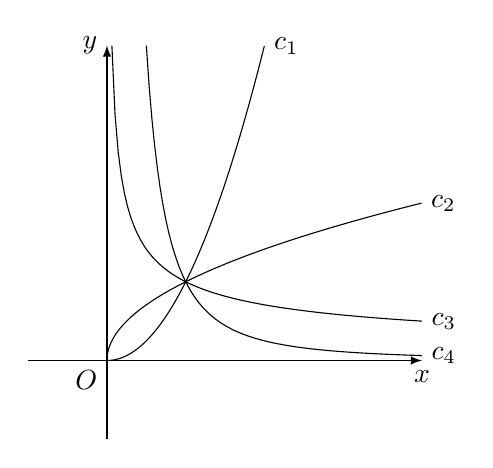
\begin{tikzpicture}[>=latex]
        \draw [->] (-1,0) -- (4,0) node [below] {$x$};
        \draw [->] (0,-1) -- (0,4) node [left] {$y$};
        \draw (0,0) node [below left] {$O$};
        \draw [domain = 0:2, samples = 100] plot (\x,\x*\x) node [right] {$c_1$};
        \draw [domain = 0:2, samples = 100] plot (\x*\x,\x) node [right] {$c_2$};
        \draw [domain = 0.0625:4, samples = 100] plot (\x, {1/sqrt(\x)}) node [right] {$c_3$};
        \draw [domain = 0.5:4, samples = 100] plot (\x, {1/\x/\x}) node [right] {$c_4$};
    \end{tikzpicture}
    \end{center}
\fourch{$-2,-\dfrac 12,\dfrac 12,2$}{$2,\dfrac 12,-\dfrac 12,-2$
}{$-\dfrac 12,-2,2,\dfrac 12$}{$2,\dfrac 12,-2,-\dfrac 12$}


关联目标:

暂未关联目标



标签: 第二单元

答案: 暂无答案

解答或提示: 暂无解答与提示

使用记录:

暂无使用记录


出处: 2022届高三第一轮复习讲义
\item { (002911)}已知$\alpha\in \{-2,-1,-\dfrac 12,\dfrac 12,1,2,3\}$, 若幂函数$f(x)=x^\alpha$为奇函数, 且在$(0,+\infty)$上递减, 则$\alpha=$\blank{50}.


关联目标:

暂未关联目标



标签: 第二单元

答案: 暂无答案

解答或提示: 暂无解答与提示

使用记录:

暂无使用记录


出处: 2022届高三第一轮复习讲义
\item { (002912)}函数$y=f(x)$满足两个条件:
\textcircled{1} $y=f(x)$是两个幂函数的和函数; \textcircled{2} $y=f(x)$的最小值为2, 则$y=f(x)$的解析式可以是\blank{50}.


关联目标:

暂未关联目标



标签: 第二单元

答案: 暂无答案

解答或提示: 暂无解答与提示

使用记录:

暂无使用记录


出处: 2022届高三第一轮复习讲义
\item { (002914)}设常数$m\in \mathbf{R}$. 若幂函数$y=(m^2-m-1)x^{m^2-2m-1}$在$(0,+\infty)$上是增函数, 则$m$的值为\blank{50}.


关联目标:

暂未关联目标



标签: 第二单元

答案: 暂无答案

解答或提示: 暂无解答与提示

使用记录:

暂无使用记录


出处: 2022届高三第一轮复习讲义
\item { (002916)}函数$y=1-(x+2)^{-2}$可以先将幂函数$y=x^{-2}$的图像向\blank{50}平移$2$个单位, 再以\blank{50}轴为对称轴作对称变换, 最后向\blank{50}平移$1$个单位.


关联目标:

暂未关联目标



标签: 第二单元

答案: 暂无答案

解答或提示: 暂无解答与提示

使用记录:

暂无使用记录


出处: 2022届高三第一轮复习讲义
\item { (002918)}设常数$t\in \mathbf{Z}$. 已知幂函数$y=(t^3-t+1){x^{\frac 13(1+2t-t^2)}}$是偶函数, 且在区间$(0,+\infty)$上是增函数, 求整数$t$的值, 并作出相应的幂函数的大致图像.


关联目标:

暂未关联目标



标签: 第二单元

答案: 暂无答案

解答或提示: 暂无解答与提示

使用记录:

暂无使用记录


出处: 2022届高三第一轮复习讲义
\item { (002921)}函数$y=-(x+1)^{-3}$的图像可以先将幂函数$y=x^{-3}$的图像向\blank{50}平移1个单位, 再以\blank{50}轴为对称轴作对称变换.


关联目标:

暂未关联目标



标签: 第二单元

答案: 暂无答案

解答或提示: 暂无解答与提示

使用记录:

暂无使用记录


出处: 2022届高三第一轮复习讲义
\item { (002922)}设$\alpha \in \{-3,-\dfrac 23,-\dfrac 12,-\dfrac 13,\dfrac 13,1,\dfrac 32,2\}$. 已知幂函数$y=x^{\alpha}$是奇函数, 且在区间$(0,+\infty)$上是减函数, 则满足条件的$\alpha$的值是\blank{50}.


关联目标:

暂未关联目标



标签: 第二单元

答案: 暂无答案

解答或提示: 暂无解答与提示

使用记录:

暂无使用记录


出处: 2022届高三第一轮复习讲义
\item { (002923)}下列关于幂函数图像及性质的叙述中, 正确的叙述的序号是\blank{50}.\\
\textcircled{1} 对于一个确定的幂函数, 第二、三象限不可能同时有该幂函数的图像上的点;\\
\textcircled{2} 若某个幂函数图像过$(-1,-1)$, 则该幂函数是奇函数;\\
\textcircled{3} 若某个幂函数在定义域上递增, 则该幂函数图像必经过原点;\\
\textcircled{4} 幂函数图像不会经过点$(-\dfrac 12,8)$以及$(-8,-4)$.


关联目标:

暂未关联目标



标签: 第二单元

答案: 暂无答案

解答或提示: 暂无解答与提示

使用记录:

暂无使用记录


出处: 2022届高三第一轮复习讲义
\item { (002924)}设$y=f(x)$与$y=g(x)$是两个不同的幂函数, 集合$M=\{x|f(x)=g(x)  \}$, 则集合$M$中的元素是\bracket{20}.
\fourch{$1$或$2$}{$1$或$3$}{$1$或$2$或$3$}{$1$或$2$或$3$或$4$}


关联目标:

暂未关联目标



标签: 第二单元

答案: 暂无答案

解答或提示: 暂无解答与提示

使用记录:

暂无使用记录


出处: 2022届高三第一轮复习讲义
\item { (002925)}已知幂函数$y=x^{\frac qp}$($p\in \mathbf{N}^*,\ q\in \mathbf{N}^*$, $p,q$互质)的图像如图所示, 则\bracket{20}.
\begin{center}
    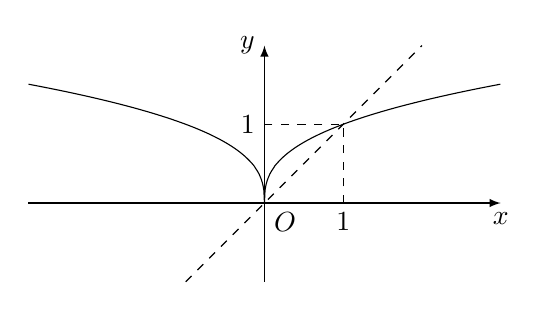
\begin{tikzpicture}[>=latex]
        \draw [->] (-3,0) -- (3,0) node [below] {$x$};
        \draw [->] (0,-1) -- (0,2) node [left] {$y$};
        \draw (0,0) node [below right] {$O$};
        \draw [dashed] (-1,-1) -- (2,2);
        \draw [domain = 0:3, samples = 400] plot (\x,{\x^(3/8)}) plot (-\x,{\x^(3/8)});
        \draw [dashed] (1,0) node [below] {$1$} -- (1,1) -- (0,1) node [left] {$1$};
    \end{tikzpicture}
\end{center}
\twoch{$p,q$均为奇数}{$p$是奇数, $q$是偶数, 且$0<\dfrac qp<1$}{$p$是偶数, $q$是奇数}{$p$是奇数, $q$是偶数, 且$\dfrac qp>1$}


关联目标:

暂未关联目标



标签: 第二单元

答案: 暂无答案

解答或提示: 暂无解答与提示

使用记录:

暂无使用记录


出处: 2022届高三第一轮复习讲义
\item { (002930)}函数$y=\log_2 \dfrac 1{x-1}$的反函数是\blank{50}.


关联目标:

暂未关联目标



标签: 第二单元

答案: 暂无答案

解答或提示: 暂无解答与提示

使用记录:

暂无使用记录


出处: 2022届高三第一轮复习讲义
\item { (002932)}函数$y=\dfrac{2^x}{{2^x}-1}$($x>0$)的反函数是\blank{50}.


关联目标:

暂未关联目标



标签: 第二单元

答案: 暂无答案

解答或提示: 暂无解答与提示

使用记录:

暂无使用记录


出处: 2022届高三第一轮复习讲义
\item { (002934)}记$y=f^{-1}(x)$是$y=f(x)$的反函数. 若函数$f(x)=\log_3x$, 则$f^{-1}(-\log_9 2)$=\blank{50}.


关联目标:

暂未关联目标



标签: 第二单元

答案: 暂无答案

解答或提示: 暂无解答与提示

使用记录:

暂无使用记录


出处: 2022届高三第一轮复习讲义
\item { (002941)}(1) 函数$y=x^2+2x-3\ (x\ge 0)$的反函数为\blank{50};\\
(2) 函数$y=\dfrac{\mathrm{e}^x-1}{{\mathrm{e}}^x+1}$的反函数为\blank{50};\\
(3) 函数$y=x|x|$的反函数为\blank{50}.


关联目标:

暂未关联目标



标签: 第二单元

答案: 暂无答案

解答或提示: 暂无解答与提示

使用记录:

暂无使用记录


出处: 2022届高三第一轮复习讲义
\item { (002942)}已知函数$y=f(x)$是奇函数, 且$y=g(x)$是$y=f(x)$的反函数. 若$x\ge 0$时, $f(x)=3^x-1$, 则$g(-8)$=\blank{50}.


关联目标:

暂未关联目标



标签: 第二单元

答案: 暂无答案

解答或提示: 暂无解答与提示

使用记录:

暂无使用记录


出处: 2022届高三第一轮复习讲义
\item { (002944)}求函数$y=\begin{cases}x^2-2x+2, & x\le 1,\\(\dfrac 12)^x, & x>1  \end{cases}$的反函数.


关联目标:

暂未关联目标



标签: 第二单元

答案: 暂无答案

解答或提示: 暂无解答与提示

使用记录:

暂无使用记录


出处: 2022届高三第一轮复习讲义
\item { (002945)}设常数$a>0$且$a\ne 1$. 求函数$f(x)=\log_a(x+\sqrt{x^2-1})$的反函数.


关联目标:

暂未关联目标



标签: 第二单元

答案: 暂无答案

解答或提示: 暂无解答与提示

使用记录:

暂无使用记录


出处: 2022届高三第一轮复习讲义
\item { (002948)}设$a>0$, 函数$f(x)=\dfrac 1{1+a\cdot 2^x}$.\\
(1) 若$a=1$, 求$f(x)$的反函数$f^{-1}(x)$;\\
(2) 求函数$y=f(x)\cdot f(-x)$的最大值(用$a$表示);\\
(3) *设$g(x)=f(x)-f(x-1)$. 若对任意$x\in (-\infty ,0]$, $g(x)\ge g(0)$恒成立, 求$a$的取值范围.


关联目标:

暂未关联目标



标签: 第二单元

答案: 暂无答案

解答或提示: 暂无解答与提示

使用记录:

暂无使用记录


出处: 2022届高三第一轮复习讲义
\item { (002950)}若$\log_35=a$, $\log_57=b$ , 用$a,b$表示$\log_{75}63=$\blank{50}.


关联目标:

暂未关联目标



标签: 第二单元

答案: 暂无答案

解答或提示: 暂无解答与提示

使用记录:

暂无使用记录


出处: 2022届高三第一轮复习讲义
\item { (002951)}若$3^a=4^b=6^c$, 且$a,b,c$都是正数, 则$\dfrac{-2ab+2bc+ac}{abc}$的值为\blank{50}.


关联目标:

暂未关联目标



标签: 第二单元

答案: 暂无答案

解答或提示: 暂无解答与提示

使用记录:

暂无使用记录


出处: 2022届高三第一轮复习讲义
\item { (002952)}若不等式$(a-1)^x<1$的解集为$(-\infty,0)$, 则实数$a$的取值范围是\blank{50}.


关联目标:

暂未关联目标



标签: 第二单元

答案: 暂无答案

解答或提示: 暂无解答与提示

使用记录:

暂无使用记录


出处: 2022届高三第一轮复习讲义
\item { (002953)}函数$f(x)=\dfrac{\sqrt{4-x^2}}{\lg |x-1|}$的定义域为\blank{50}.


关联目标:

暂未关联目标



标签: 第二单元

答案: 暂无答案

解答或提示: 暂无解答与提示

使用记录:

暂无使用记录


出处: 2022届高三第一轮复习讲义
\item { (002954)}为了得到函数$y=\lg\dfrac{x+3}{10}$的图像, 只需把函数$y=\lg x$的图像上所有的点\bracket{20}.
\onech{向左平移$3$个单位长度, 再向上平移$1$个单位长度}{向右平移$3$个单位长度, 再向上平移$1$个单位长度}{向左平移$3$个单位长度, 再向下平移$1$个单位长度}{向右平移$3$个单位长度, 再向下平移$1$个单位长度}


关联目标:

暂未关联目标



标签: 第二单元

答案: 暂无答案

解答或提示: 暂无解答与提示

使用记录:

暂无使用记录


出处: 2022届高三第一轮复习讲义
\item { (002955)}设常数$a>0,\ a\ne 1$. 函数$f(x)=a^x$在$[0,1]$上的最大值和最小值之和为$a^2$, 则$a=$\blank{50}.


关联目标:

暂未关联目标



标签: 第二单元

答案: 暂无答案

解答或提示: 暂无解答与提示

使用记录:

暂无使用记录


出处: 2022届高三第一轮复习讲义
\item { (002956)}若集合$A=\{y|y=2\cdot (\dfrac 13)^{|x|}\}$, $B=\{ a|\log_a(3a-1)>0\}$, 则$A\cap B$=\blank{50}.


关联目标:

暂未关联目标



标签: 第二单元

答案: 暂无答案

解答或提示: 暂无解答与提示

使用记录:

暂无使用记录


出处: 2022届高三第一轮复习讲义
\item { (002957)}*已知函数$f(x)=|3^x-1|$, $c<b<a$, 且$f(b)<f(a)<f(c)$, 在下列关系式中, 一定成立的关系式的序号是\blank{50}.
\textcircled{1} $3^a+3^b>2$; \textcircled{2} $3^a+3^b<2$; \textcircled{3} $3^c<1$; \textcircled{4} $3^a+3^c<2$.


关联目标:

暂未关联目标



标签: 第二单元

答案: 暂无答案

解答或提示: 暂无解答与提示

使用记录:

暂无使用记录


出处: 2022届高三第一轮复习讲义
\item { (002958)}已知函数$f(x)=\dfrac{3^x-3^{-x}}{3^x+3^{-x}}$.\\
(1) 证明$f(x)$在$(-\infty,+\infty)$上是增函数;\\
(2) 求$f(x)$的值域.


关联目标:

暂未关联目标



标签: 第二单元

答案: 暂无答案

解答或提示: 暂无解答与提示

使用记录:

暂无使用记录


出处: 2022届高三第一轮复习讲义
\item { (002959)}已知函数$y=(\log_2\dfrac x{2^a})(\log_2\dfrac x4)$, $x\in [\sqrt 2,4]$, 试求该函数的最大值$g(a)$.


关联目标:

暂未关联目标



标签: 第二单元

答案: 暂无答案

解答或提示: 暂无解答与提示

使用记录:

暂无使用记录


出处: 2022届高三第一轮复习讲义
\item { (002960)}已知函数$f(x)=a\cdot 2^x+b\cdot 3^x$, 其中常数$a,b$满足$ab\ne 0$.\\
(1) 若$ab>0$, 判断函数$y=f(x)$的单调性;\\
(2) 若$ab<0$, 求$f(x+1)>f(x)$时$x$的取值范围.


关联目标:

暂未关联目标



标签: 第二单元

答案: 暂无答案

解答或提示: 暂无解答与提示

使用记录:

暂无使用记录


出处: 2022届高三第一轮复习讲义
\item { (002961)}不等式$\log_{\frac 12}(x-1)\ge 1$的解集为\blank{50}.


关联目标:

暂未关联目标



标签: 第二单元

答案: 暂无答案

解答或提示: 暂无解答与提示

使用记录:

暂无使用记录


出处: 2022届高三第一轮复习讲义
\item { (002962)}设常数$a\in \mathbf{R}$. 若函数$f(x)=\dfrac 1{2^x-1}+a$为奇函数, 则$a$=\blank{50}.


关联目标:

暂未关联目标



标签: 第二单元

答案: 暂无答案

解答或提示: 暂无解答与提示

使用记录:

暂无使用记录


出处: 2022届高三第一轮复习讲义
\item { (002963)}若$\log_23=a$, $3^b=7$, 用$a,b$表示$\log_{3\sqrt 7}2$, 则$\log_{3\sqrt 7}2$=\blank{50}.


关联目标:

暂未关联目标



标签: 第二单元

答案: 暂无答案

解答或提示: 暂无解答与提示

使用记录:

暂无使用记录


出处: 2022届高三第一轮复习讲义
\item { (002964)}对于函数$y=f(x)$的定义域中的任意的$x_1,x_2$($x_1\ne x_2$), 有如下结论:\\
\textcircled{1} $f(x_1+x_2)=f(x_1)\cdot f(x_2)$; \textcircled{2} $f(x_1\cdot x_2)=f(x_1)+f(x_2)$;\\ \textcircled{3} $\dfrac{f(x_1)-f(x_2)}x_1-x_2>0$; \textcircled{4} $f(\dfrac{x_1+x_2}2)<\dfrac{f(x_1)+f(x_2)}2$. 
\\当$y=\ln x$时, 上述结论中, 正确结论的序号是\blank{50}.


关联目标:

暂未关联目标



标签: 第二单元

答案: 暂无答案

解答或提示: 暂无解答与提示

使用记录:

暂无使用记录


出处: 2022届高三第一轮复习讲义
\item { (002965)}(1) *函数$y=\log_a|x-b|$在$(0,+\infty)$上递增, 则$a$、$b$满足\bracket{20}.
\fourch{$a>1$且$b\ge 0$}{$a>1$且$b\le 0$}{$0<a<1$且$b\ge 0$}{$0<a<1$且$b\le 0$}
(2) 函数$f(x)=\log_a|ax^2-x| \ (a>0,\ a\ne 1)$在区间$[3,4]$上是增函数, 则实数$a$的范围是\blank{50}.


关联目标:

暂未关联目标



标签: 第二单元

答案: 暂无答案

解答或提示: 暂无解答与提示

使用记录:

暂无使用记录


出处: 2022届高三第一轮复习讲义
\item { (002966)}*已知常数$a>1$, 函数$y=|\log_ax|$的定义域为区间$[m,n]$, 值域为区间$[0,1]$. 若$n-m$的最小值为$\dfrac 56$, 则$a$=\blank{50}.


关联目标:

暂未关联目标



标签: 第二单元

答案: 暂无答案

解答或提示: 暂无解答与提示

使用记录:

暂无使用记录


出处: 2022届高三第一轮复习讲义
\item { (002967)}*设常数$a>0$ ,$a\ne 1$. 已知函数$f(x)=\log_ax$. 若对于任意$x\in [3,+\infty)$都有$|f(x)|\ge 1$成立, 则$a$的取值范围为\blank{50}.


关联目标:

暂未关联目标



标签: 第二单元

答案: 暂无答案

解答或提示: 暂无解答与提示

使用记录:

暂无使用记录


出处: 2022届高三第一轮复习讲义
\item { (002968)}*已知函数$f(x)=2+\log_3 x\ (3\le x\le 27)$.\\
(1) 求函数$y=f(x^2)$的定义域;\\
(2) 求函数$g(x)={[f(x)]}^2+f(x^2)$的值域.


关联目标:

暂未关联目标



标签: 第二单元

答案: 暂无答案

解答或提示: 暂无解答与提示

使用记录:

暂无使用记录


出处: 2022届高三第一轮复习讲义
\item { (002969)}已知定义域为$\mathbf{R}$的函数$y=f(x)$为奇函数, 且满足$f(x+2)=-f(x)$. 当$x\in [0,1]$时, $f(x)=2^x-1$.\\
(1) 求$y=f(x)$在区间$[-1,0)$上的解析式;\\
(2) 求$f(\log_{\frac 12}24)$的值.


关联目标:

暂未关联目标



标签: 第二单元

答案: 暂无答案

解答或提示: 暂无解答与提示

使用记录:

暂无使用记录


出处: 2022届高三第一轮复习讲义
\item { (002970)}*已知函数$f(x)=1+a\cdot (\dfrac 12)^x+(\dfrac 14)^x$.\\
(1) 当$a=1$时, 求函数$y=f(x)$在$(-\infty,0)$上的值域;\\
(2) 对于定义在集合$D$上的函数$y=f(x)$, 如果存在常数$M>0$, 满足: 对任意$x\in D$, 都有$|f(x)|\le M$成立, 则称$f(x)$是$D$上的有界函数, 其中$M$称为函数$f(x)$的一个上界.若函数$y=f(x)$在$[0,+\infty)$上是以$3$为一个上界的有界函数, 求实数$a$的取值范围.


关联目标:

暂未关联目标



标签: 第二单元

答案: 暂无答案

解答或提示: 暂无解答与提示

使用记录:

暂无使用记录


出处: 2022届高三第一轮复习讲义
\item { (002980)}已知函数$y=x+\dfrac ax$有如下性质: 如果常数$a>0$, 那么该函数在$(0, \sqrt a]$上是减函数, 在$[\sqrt a, +\infty)$上是增函数.\\
(1) 设常数$c\in [1,+\infty)$, 求函数$f(x)=x+\dfrac cx \ (1\le x\le 2)$的最大值和最小值;\\
(2) *设常数$c>0$. 当$n$是正整数时, 研究函数$g(x)=x^n+\dfrac c{x^n}$的单调性, 并说明理由.


关联目标:

暂未关联目标



标签: 第二单元

答案: 暂无答案

解答或提示: 暂无解答与提示

使用记录:

暂无使用记录


出处: 2022届高三第一轮复习讲义
\item { (002993)}函数$y=\dfrac{3^x-1}{3^x-2}$的值域是\blank{50}.


关联目标:

暂未关联目标



标签: 第二单元

答案: 暂无答案

解答或提示: 暂无解答与提示

使用记录:

暂无使用记录


出处: 2022届高三第一轮复习讲义
\item { (002994)}函数$y=\log_{\frac 12}(-x^2+2x+3)$的值域是\blank{50}.


关联目标:

暂未关联目标



标签: 第二单元

答案: 暂无答案

解答或提示: 暂无解答与提示

使用记录:

暂无使用记录


出处: 2022届高三第一轮复习讲义
\item { (003000)}已知函数$f(x)=\log_a(x+\sqrt{x^2+1}), \ a>1$.\\
(1) 求$f(x)$的定义域和值域;\\
(2) 求$f^{-1}(x)$;\\
(3) 判断$f^{-1}(x)$的奇偶性、单调性;\\
(4) 若实数$m$满足$f^{-1}(1-m)+f^{-1}(1-m^2)<0$, 求$m$的范围.


关联目标:

暂未关联目标



标签: 第二单元

答案: 暂无答案

解答或提示: 暂无解答与提示

使用记录:

暂无使用记录


出处: 2022届高三第一轮复习讲义
\item { (003014)}用二分法, 可以计算得方程$6-x=\lg x$的解是\blank{50}(结果精确到0.01).


关联目标:

暂未关联目标



标签: 第二单元

答案: 暂无答案

解答或提示: 暂无解答与提示

使用记录:

暂无使用记录


出处: 2022届高三第一轮复习讲义
\item { (003015)}方程$6-x=\log_2 x$的解集是\blank{50}.


关联目标:

暂未关联目标



标签: 第二单元

答案: 暂无答案

解答或提示: 暂无解答与提示

使用记录:

暂无使用记录


出处: 2022届高三第一轮复习讲义
\item { (003017)}若方程$2^x=(\dfrac 12)^{-\frac 1x+1}$的两个实数解为$x_1, x_2$, 则$x_1+x_2$=\blank{50}.


关联目标:

暂未关联目标



标签: 第二单元

答案: 暂无答案

解答或提示: 暂无解答与提示

使用记录:

暂无使用记录


出处: 2022届高三第一轮复习讲义
\item { (003018)}设常数$a\in \mathbf{R}$. 若关于$x$的方程$\lg^2x-\lg x^2+a-2=0$有两个不同的实数解$x_1, x_2$, 则\\
(1) $x_1\cdot x_2$=\blank{50};\\
(2) $a$的取值范围是\blank{50}.


关联目标:

暂未关联目标



标签: 第二单元

答案: 暂无答案

解答或提示: 暂无解答与提示

使用记录:

暂无使用记录


出处: 2022届高三第一轮复习讲义
\item { (003019)}(1) 设常数$a\in \mathbf{R}$. 若关于$x$的方程$9^x-(a+2)\cdot 3^x+4=0$有实数解, 则$a$的取值范围是\blank{50};\\
(2)设常数$a\in \mathbf{R}$.若关于$x$的方程$9^x-3^x+a=0$有两个不同的实数解$x_1, x_2$, 则$a$的取值范围是\blank{50}.


关联目标:

暂未关联目标



标签: 第二单元

答案: 暂无答案

解答或提示: 暂无解答与提示

使用记录:

暂无使用记录


出处: 2022届高三第一轮复习讲义
\item { (003024)}方程$4^{x+1}-13\cdot 2^x+3=0$的解集是\blank{50}.


关联目标:

暂未关联目标



标签: 第二单元

答案: 暂无答案

解答或提示: 暂无解答与提示

使用记录:

暂无使用记录


出处: 2022届高三第一轮复习讲义
\item { (003025)}方程$\log_2(x-1)=\log_4(2-x)$的解集是\blank{50}.


关联目标:

暂未关联目标



标签: 第二单元

答案: 暂无答案

解答或提示: 暂无解答与提示

使用记录:

暂无使用记录


出处: 2022届高三第一轮复习讲义
\item { (003026)}方程$2\log_2(x-1)=2+\log_2 x$的解集是\blank{50}.


关联目标:

暂未关联目标



标签: 第二单元

答案: 暂无答案

解答或提示: 暂无解答与提示

使用记录:

暂无使用记录


出处: 2022届高三第一轮复习讲义
\item { (003027)}方程$\log_3(3^{x-1}-3^{-1})\cdot \log_3(3^{x-2}-3^{-2})=2$的解集是\blank{50}.


关联目标:

暂未关联目标



标签: 第二单元

答案: 暂无答案

解答或提示: 暂无解答与提示

使用记录:

暂无使用记录


出处: 2022届高三第一轮复习讲义
\item { (003029)}方程$2(4^x+4^{-x})-3(2^x-2^{-x})-4=0$的解集是\blank{50}.


关联目标:

暂未关联目标



标签: 第二单元

答案: 暂无答案

解答或提示: 暂无解答与提示

使用记录:

暂无使用记录


出处: 2022届高三第一轮复习讲义
\item { (003032)}设常数$a\in \mathbf{R}$.已知函数$f(x)=4^x-a\cdot 2^x+a+3$.\\
(1) 若函数$y=f(x)$有且仅有一个零点, 求$a$的取值范围;\\
(2) 若函数$y=f(x)$有零点, 求$a$的取值范围.


关联目标:

暂未关联目标



标签: 第二单元

答案: 暂无答案

解答或提示: 暂无解答与提示

使用记录:

暂无使用记录


出处: 2022届高三第一轮复习讲义
\item { (003041)}已知实数$ab$满足等式$(\dfrac 12)^a=(\dfrac 13)^b$, 下列五个关系式:\\
\textcircled{1} $0<b<a$; \textcircled{2} $a<b<0$; \textcircled{3} $0<a<b$; \textcircled{4} $b<a<0$; \textcircled{5} $a=b=0$. 其中不可能成立的关系式的序号为\blank{50}.


关联目标:

暂未关联目标



标签: 第二单元

答案: 暂无答案

解答或提示: 暂无解答与提示

使用记录:

暂无使用记录


出处: 2022届高三第一轮复习讲义
\item { (003043)}设常数$k\in \mathbf{R}$. 已知关于x的不等式$k\cdot 4^x-2^{x+1}+6k<0$.\\
(1) 若不等式的解集为开区间$(1, \log_2 3)$, 求$k$的取值范围;\\
(2) 若不等式对一切$x\in (1,\log_2 3)$都成立, 求$k$的取值范围;\\
(3) *若不等式的解集为开区间$(1,\log_2 3)$的子集, 求$k$的取值范围;\\
(4) *若不等式在开区间$(1,\log_2 3)$内存在解, 求$k$的取值范围.


关联目标:

暂未关联目标



标签: 第二单元

答案: 暂无答案

解答或提示: 暂无解答与提示

使用记录:

暂无使用记录


出处: 2022届高三第一轮复习讲义
\item { (003052)}设常数$a\in \mathbf{R}$.若对于任意实数$x\in (-\infty ,-1]$, 不等式$1+2^x+(a-a^2)\cdot 4^x>0$恒成立, 求$a$的取值范围.


关联目标:

暂未关联目标



标签: 第二单元

答案: 暂无答案

解答或提示: 暂无解答与提示

使用记录:

暂无使用记录


出处: 2022届高三第一轮复习讲义
\item { (003601)}下列函数中, 既是奇函数又是减函数的是\bracket{20}.
\fourch{$y=-3x$}{$y=x^3$}{$y=\log_3^x$}{$y=3^x$}


关联目标:

暂未关联目标



标签: 第二单元

答案: 暂无答案

解答或提示: 暂无解答与提示

使用记录:

暂无使用记录


出处: 上海2021年秋季高考试题13
\item { (003636)}已知函数$f(x)$的周期为$1$, 当$0<x\le 1$时, $f(x)=\log_2 x$, 则$f\left(\dfrac{3}{2}\right)$的值为\blank{50}.


关联目标:

暂未关联目标



标签: 第二单元

答案: 暂无答案

解答或提示: 暂无解答与提示

使用记录:

暂无使用记录


出处: 上海2019年秋季高考试题6
\item { (003655)}设常数$a\in \mathbf{R}$, 函数$f(x)=\log_2(x+a)$. 若$f(x)$的反函数的图像经过点$(3,1)$, 则$a=$\blank{50}.


关联目标:

暂未关联目标



标签: 第二单元

答案: 暂无答案

解答或提示: 暂无解答与提示

使用记录:

暂无使用记录


出处: 上海2018年秋季高考试题4
\item { (003658)}已知$\alpha\in \left\{-2,-1,-\dfrac{1}{2},\dfrac{1}{2},1,2,3\right\}$. 若幂函数$f(x)=x^{\alpha}$为奇函数, 且在$(0,+\infty)$上递减, 则$\alpha=$\blank{50}.


关联目标:

暂未关联目标



标签: 第二单元

答案: 暂无答案

解答或提示: 暂无解答与提示

使用记录:

暂无使用记录


出处: 上海2018年秋季高考试题7
\item { (003662)}已知常数$a>0$, 函数$f(x)=\dfrac{2^x}{2^x+ax}$的图像经过点$P\left(p,\dfrac{6}{5}\right)$, $Q\left(q,-\dfrac{1}{5}\right)$. 若$2^{p+q}=36pq$, 则$a=$\blank{50}.


关联目标:

暂未关联目标



标签: 第二单元

答案: 暂无答案

解答或提示: 暂无解答与提示

使用记录:

20220630	2022届高三1班	\fcolorbox[rgb]{0,0,0}{1.000,0.000,0}{1.000}


出处: 上海2018年秋季高考试题11
\item { (003680)}定义在$(0,+\infty)$上的函数$y=f(x)$的反函数为$y=f^{-1}(x)$. 若$g(x)=\begin{cases}3^x-1, & x\le 0,\\ f(x), & x>0\end{cases}$为奇函数, 则$f^{-1}(x)=2$的解为\blank{50}.


关联目标:

暂未关联目标



标签: 第二单元

答案: 暂无答案

解答或提示: 暂无解答与提示

使用记录:

暂无使用记录


出处: 上海2017年秋季高考试题8
\item { (003694)}已知函数$f(x)=\log_a x+x-b$($a>0$且$a\ne 1$). 当$2<a<3<b<4$时, 函数$f(x)$的零点$x_0\in (n,n+1), \ n\in \mathbf{N}^*$, 则$n=$\blank{50}.


关联目标:

暂未关联目标



标签: 第二单元

答案: 暂无答案

解答或提示: 暂无解答与提示

使用记录:

暂无使用记录


出处: 2022届高三高考前冲刺题精选
\item { (003709)}若函数$y=a^x+b$($a>0$且$a\ne 1$)的图像经过点$(1,7)$, 其反函数的图像经过点$(4,0)$, 则$a-b=$\blank{50}.


关联目标:

暂未关联目标



标签: 第二单元

答案: 暂无答案

解答或提示: 暂无解答与提示

使用记录:

暂无使用记录


出处: 2016年双基百分百
\item { (003718)}已知函数$f(x)=\begin{cases}
\log_2(x+4), & x\ge 0,\\f(x+1)-f(x+2), & x<0,\end{cases}$ 则$f(-3)$的值为\blank{30}.
\fourch{$1$}{$0$}{$2$}{$-2$}


关联目标:

暂未关联目标



标签: 第二单元

答案: 暂无答案

解答或提示: 暂无解答与提示

使用记录:

暂无使用记录


出处: 2016年双基百分百
\item { (003726)}若函数$f(x)=\dfrac{k-2^x}{1+k\cdot 2^x}, \ (k\ne 1, \ k\in \mathbf{R})$在定义域内为奇函数, 则$k=$\blank{50}.


关联目标:

暂未关联目标



标签: 第二单元

答案: 暂无答案

解答或提示: 暂无解答与提示

使用记录:

暂无使用记录


出处: 2016年双基百分百
\item { (003730)}下列函数中, 与函数$y=x^{2n+1} \ (n\in \mathbf{N}^*)$的值域相同的函数为\blank{30}.
\fourch{$y=\left(\dfrac 12\right)^{x+1}$}{$y=\ln(x+1)$}{$y=\dfrac{x+1}{x}$}{$y=x+\dfrac 1x$}


关联目标:

暂未关联目标



标签: 第二单元

答案: 暂无答案

解答或提示: 暂无解答与提示

使用记录:

暂无使用记录


出处: 2016年双基百分百
\item { (003746)}幂函数$f(x)$的图像经过点$(2,\sqrt{2})$, 且$f^{-1}(x)$为$f(x)$的反函数, 则$f^{-1}(4)=$\blank{50}.


关联目标:

暂未关联目标



标签: 第二单元

答案: 暂无答案

解答或提示: 暂无解答与提示

使用记录:

暂无使用记录


出处: 2016年双基百分百
\item { (003747)}若$\log_a \dfrac 23<1 \ (a>0, \ a\ne 1)$, 则实数$a$的取值范围为\blank{50}.


关联目标:

暂未关联目标



标签: 第二单元

答案: 暂无答案

解答或提示: 暂无解答与提示

使用记录:

暂无使用记录


出处: 2016年双基百分百
\item { (003757)}设函数$f(x)=x^3+\dfrac{2^x-1}{2^x+1}$, 已知$a\in (-1,1)$, $b\in (-1,1)$. 则$a+b\ge 0$是$f(a)+f(b)\ge 0$的\blank{30}.
\twoch{充分不必要条件}{必要不充分条件}{充分必要条件}{既不充分也不必要条件}


关联目标:

暂未关联目标



标签: 第二单元

答案: 暂无答案

解答或提示: 暂无解答与提示

使用记录:

暂无使用记录


出处: 2016年双基百分百
\item { (003770)}函数$f(x)=2^x+x^3-2$在区间$(0,1)$内的零点的个数是\blank{30}.
\fourch{$0$}{$1$}{$2$}{$3$}


关联目标:

暂未关联目标



标签: 第二单元

答案: 暂无答案

解答或提示: 暂无解答与提示

使用记录:

暂无使用记录


出处: 2016年双基百分百
\item { (003772)}定义在$(-\infty,0)\cup (0,+\infty)$上的函数$f(x)$, 如果对于任意给定的等比数列$\{a_n\}$, $\{f(a_n)\}$仍是等比数列, 则称$f(x)$为``保等比数列函数''. 现有定义在$(-\infty,0)\cup (0,+\infty)$上的如下函数: \textcircled{1} $f(x)=x^2$; \textcircled{2} $f(x)=2^x$; \textcircled{3} $f(x)=\sqrt{|x|}$; \textcircled{4} $f(x)=\ln|x|$. 则其中是``保等比数列函数''的$f(x)$的序号为\blank{30}.
\fourch{\textcircled{1}\textcircled{2}}{\textcircled{3}\textcircled{4}}{\textcircled{1}\textcircled{3}}{\textcircled{2}\textcircled{4}}


关联目标:

暂未关联目标



标签: 第二单元|第四单元

答案: 暂无答案

解答或提示: 暂无解答与提示

使用记录:

暂无使用记录


出处: 2016年双基百分百
\item { (003775)}已知$U=\left\{y\left|y=\log_\frac 12 x, \ x\ge \dfrac 18\right.\right\}$, $A=\left\{x\left|y=\dfrac{1}{\sqrt{2-x}}\right.\right\}$, 则$\complement_U A=$\blank{50}.


关联目标:

暂未关联目标



标签: 第一单元|第二单元

答案: 暂无答案

解答或提示: 暂无解答与提示

使用记录:

暂无使用记录


出处: 2016年双基百分百
\item { (003778)}已知函数$f(x)=4^x-k\cdot 2^{x+1}+4$在$[0,2]$上存在零点, 则实数$k\in$\blank{50}.


关联目标:

暂未关联目标



标签: 第二单元

答案: 暂无答案

解答或提示: 暂无解答与提示

使用记录:

暂无使用记录


出处: 2016年双基百分百
\item { (003789)}设函数$f(x)=\log_\frac 12 x$, $g(x)=f^{-1}(|x|)$.\\
(1) 求函数$g(x)$的解析式, 并画出大致图像;\\
(2) 若不等式$g(x)+g(2x)\le k$对任意$x\in \mathbf{R}$恒成立, 求实数$k$的取值范围.


关联目标:

暂未关联目标



标签: 第二单元

答案: 暂无答案

解答或提示: 暂无解答与提示

使用记录:

暂无使用记录


出处: 2016年双基百分百
\item { (003801)}下列函数中, 既是偶函数, 又是在区间$(0,+\infty)$上单调递减的函数为\blank{30}.
\fourch{$y=\lg\dfrac{1}{|x|}$}{$y=x^3$}{$y=3^{|x|}$}{$y=x^2$}


关联目标:

暂未关联目标



标签: 第二单元

答案: 暂无答案

解答或提示: 暂无解答与提示

使用记录:

暂无使用记录


出处: 2016年双基百分百
\item { (003815)}在同一坐标系中画出函数$y=\log_a x, \ y=a^x, y=x+a$的图像, 可能正确的是\blank{30}.
\fourch{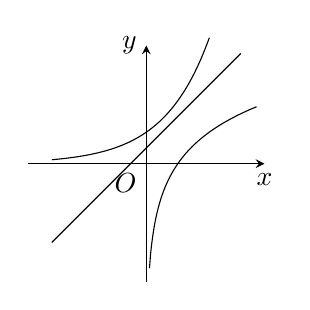
\begin{tikzpicture}[>=stealth,samples=100]
	\draw [->] (-1.5,0)--(0,0) node [below left] {$O$}--(1.5,0) node [below] {$x$};
	\draw [->] (0,-1.5)--(0,1.5) node [left] {$y$};
	\draw [domain=-3:3] plot ({\x*0.4},{(\x+0.5)*0.4});
	\draw [domain=-3:2] plot ({\x*0.4},{exp(\x*ln(2))*0.4});
	\draw [domain=0.1:3.5] plot ({\x*0.4},{ln(\x)/ln(2)*0.4});
	\end{tikzpicture}}{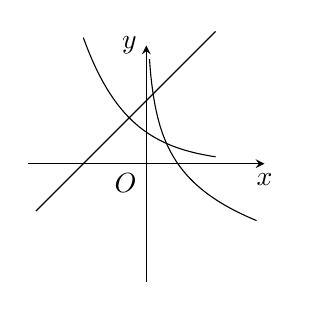
\begin{tikzpicture}[>=stealth,samples=100]
	\draw [->] (-1.5,0)--(0,0) node [below left] {$O$}--(1.5,0) node [below] {$x$};
	\draw [->] (0,-1.5)--(0,1.5) node [left] {$y$};
	\draw [domain=-3.5:2.2] plot ({\x*0.4},{(\x+2)*0.4});
	\draw [domain=-2:2.2] plot ({\x*0.4},{exp(\x*ln(1/2))*0.4});
	\draw [domain=0.1:3.5] plot ({\x*0.4},{-ln(\x)/ln(2)*0.4});
	\end{tikzpicture}}{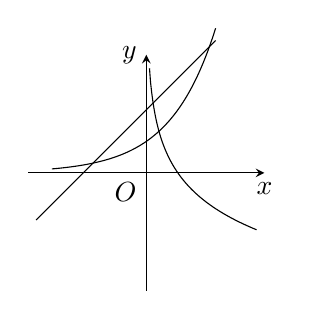
\begin{tikzpicture}[>=stealth,samples=100]
	\draw [->] (-1.5,0)--(0,0) node [below left] {$O$}--(1.5,0) node [below] {$x$};
	\draw [->] (0,-1.5)--(0,1.5) node [left] {$y$};
	\draw [domain=-3.5:2.2] plot ({\x*0.4},{(\x+2)*0.4});
	\draw [domain=-3:2.2] plot ({\x*0.4},{exp(\x*ln(2))*0.4});
	\draw [domain=0.1:3.5] plot ({\x*0.4},{-ln(\x)/ln(2)*0.4});
	\end{tikzpicture}}{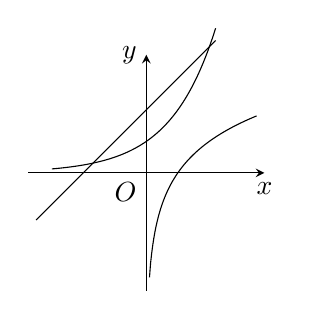
\begin{tikzpicture}[>=stealth,samples=100]
	\draw [->] (-1.5,0)--(0,0) node [below left] {$O$}--(1.5,0) node [below] {$x$};
	\draw [->] (0,-1.5)--(0,1.5) node [left] {$y$};
	\draw [domain=-3.5:2.2] plot ({\x*0.4},{(\x+2)*0.4});
	\draw [domain=-3:2.2] plot ({\x*0.4},{exp(\x*ln(2))*0.4});
	\draw [domain=0.1:3.5] plot ({\x*0.4},{ln(\x)/ln(2)*0.4});
	\end{tikzpicture}}


关联目标:

暂未关联目标



标签: 第二单元

答案: 暂无答案

解答或提示: 暂无解答与提示

使用记录:

暂无使用记录


出处: 2016年双基百分百
\item { (003828)}已知正数$x,y$满足$\ln x+\ln y=\ln (x+y)$, 则$2x+y$的最小值是\blank{50}.


关联目标:

暂未关联目标



标签: 第一单元|第二单元

答案: 暂无答案

解答或提示: 暂无解答与提示

使用记录:

暂无使用记录


出处: 2016年双基百分百
\item { (003838)}已知函数$f(x)=\begin{cases}
\dfrac 3x, & x\ge 3,\\ \log_3 x, & 0<x<3,
\end{cases}$ 若关于$x$的方程$f(x)=k$有两个不同的实根, 则实数$k$的取值范围是\blank{50}.


关联目标:

暂未关联目标



标签: 第二单元

答案: 暂无答案

解答或提示: 暂无解答与提示

使用记录:

暂无使用记录


出处: 2016年双基百分百
\item { (003854)}不等式$\lg(-x)<x+1$的解集为\blank{50}.


关联目标:

暂未关联目标



标签: 第二单元

答案: 暂无答案

解答或提示: 暂无解答与提示

使用记录:

暂无使用记录


出处: 2016年双基百分百
\item { (003865)}集合$\{y|y=2^{-x}\}\cap\{y|y=\lg x, \ 0<x<100\}=$\blank{50}.


关联目标:

暂未关联目标



标签: 第二单元

答案: 暂无答案

解答或提示: 暂无解答与提示

使用记录:

暂无使用记录


出处: 2016年双基百分百
\item { (003869)}函数$f(x)=a^x+b \ (a>1, \ b<-1)$, 则$y=f^{-1}(x)$的图像一定不经过第\blank{50}象限.


关联目标:

暂未关联目标



标签: 第二单元

答案: 暂无答案

解答或提示: 暂无解答与提示

使用记录:

暂无使用记录


出处: 2016年双基百分百
\item { (003911)}已知函数$f(x)=\begin{cases}
2^x-1, & x\ge 0,\\ -x^2-2x, & x<0,
\end{cases}$ 若$f(a)=1$, 则实数$a$的值是\blank{50}.


关联目标:

暂未关联目标



标签: 第二单元

答案: 暂无答案

解答或提示: 暂无解答与提示

使用记录:

暂无使用记录


出处: 2016年双基百分百
\item { (003936)}函数$y=\ln(\cos x) \ \left(-\dfrac{\pi}{2}<x<\dfrac{\pi}{2}\right)$的大致图像是\blank{30}.
\fourch{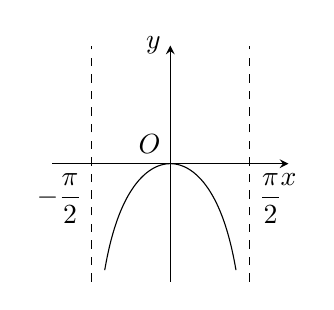
\begin{tikzpicture}[samples=200,>=stealth]
	\draw [->](-1.5,0)--(0,0) node [above left] {$O$}--(1.5,0) node [below] {$x$};
	\draw [->](0,-1.5)--(0,1.5) node [left] {$y$};
	\draw [dashed] (-1,-1.5)--(-1,1.5) (1,-1.5)--(1,1.5);
	\draw (-1,0) node [below left] {$-\dfrac{\pi}{2}$};
	\draw (1,0) node  [below right] {$\dfrac{\pi}{2}$};
	\draw [domain=-75:75] plot ({\x/90},{ln(cos(\x))});
	\end{tikzpicture}}{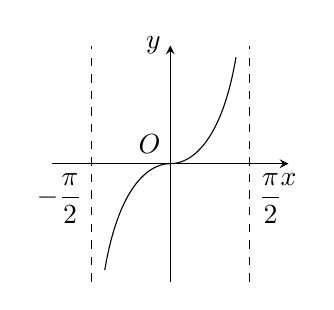
\begin{tikzpicture}[samples=200,>=stealth]
	\draw [->](-1.5,0)--(0,0) node [above left] {$O$}--(1.5,0) node [below] {$x$};
	\draw [->](0,-1.5)--(0,1.5) node [left] {$y$};
	\draw [dashed] (-1,-1.5)--(-1,1.5) (1,-1.5)--(1,1.5);
	\draw (-1,0) node [below left] {$-\dfrac{\pi}{2}$};
	\draw (1,0) node  [below right] {$\dfrac{\pi}{2}$};
	\draw [domain=-75:0] plot ({\x/90},{ln(cos(\x))});
	\draw [domain=0:75] plot ({\x/90},{-ln(cos(\x))});
	\end{tikzpicture}}{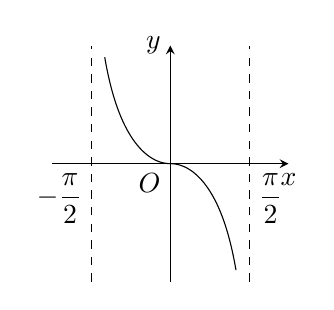
\begin{tikzpicture}[samples=200,>=stealth]
	\draw [->](-1.5,0)--(0,0) node [below left] {$O$}--(1.5,0) node [below] {$x$};
	\draw [->](0,-1.5)--(0,1.5) node [left] {$y$};
	\draw [dashed] (-1,-1.5)--(-1,1.5) (1,-1.5)--(1,1.5);
	\draw (-1,0) node [below left] {$-\dfrac{\pi}{2}$};
	\draw (1,0) node  [below right] {$\dfrac{\pi}{2}$};
	\draw [domain=-75:0] plot ({\x/90},{-ln(cos(\x))});
	\draw [domain=0:75] plot ({\x/90},{ln(cos(\x))});
	\end{tikzpicture}}{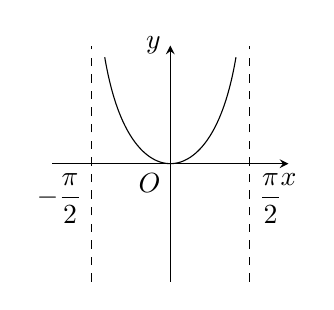
\begin{tikzpicture}[samples=200,>=stealth]
	\draw [->](-1.5,0)--(0,0) node [below left] {$O$}--(1.5,0) node [below] {$x$};
	\draw [->](0,-1.5)--(0,1.5) node [left] {$y$};
	\draw [dashed] (-1,-1.5)--(-1,1.5) (1,-1.5)--(1,1.5);
	\draw (-1,0) node [below left] {$-\dfrac{\pi}{2}$};
	\draw (1,0) node  [below right] {$\dfrac{\pi}{2}$};
	\draw [domain=-75:75] plot ({\x/90},{-ln(cos(\x))});
	\end{tikzpicture}}


关联目标:

暂未关联目标



标签: 第二单元

答案: 暂无答案

解答或提示: 暂无解答与提示

使用记录:

暂无使用记录


出处: 2016年双基百分百
\item { (003953)}已知集合$M$是满足下列性质的函数$f(x)$的全体, 存在非零常数$T$, 对任意$x\in \mathbf{R}$, 有$f(x+T)=Tf(x)$成立.\\
(1) 函数$f(x)=x$是否属于集合$M$? 说明理由;\\
(2) 设$f(x)\in M$, 且$T=2$, 已知当$1<x<2$时, $f(x)=x+\ln x$, 求当$-3<x<-2$时, $f(x)$的解析式.


关联目标:

暂未关联目标



标签: 第二单元

答案: 暂无答案

解答或提示: 暂无解答与提示

使用记录:

暂无使用记录


出处: 2016年双基百分百
\item { (004001)}已知$f(x)=\sqrt{x}$, $g(x)=kx^x$.\\
(1) 求曲线$y=f(x)$在点$(4,2)$处的切线方程;\\
(2) 若曲线$y=g(x)$经过点$(4,2)$, 求它与(1)中切线的另一个交点.


关联目标:

K0228004X|D02005X|会通过求导, 求得不超过二次的多项式函数在图像上一点处的切线方程.

K0228001X|D02005X|了解一般曲线的切线可定义为割线的极限情形.



标签: 第二单元

答案: 暂无答案

解答或提示: 暂无解答与提示

使用记录:

暂无使用记录


出处: 教材复习题
\item { (004003)}已知$f(x)=lnx$, $g(x)=\mathrm{e}^x$, 计算下列函数$y=h(x)$在点$x=1$处的导数值:\\
(1) $h(x)=3f(x)-5g(x)$;\\
(2) $h(x)=f(x)g(x)$;\\
(3) $h(x)=\dfrac{f(x)}{g(x)}$;\\
(4) $h(x)=f(2x+1)+g(3x-1)$.


关联目标:

K0229004X|D02005X|了解幂函数, $f(x)=\mathrm{e}^x$, $f(x)=\ln x$, 正弦函数与余弦函数的导数.

K0230004X|D02005X|会将简单的初等函数表达为若干个基本初等函数的四则运算, 并用导数的四则运算法则求导.

K0231003X|D02005X|会结合使用$f(ax+b)$型复合函数的求导法则及四则运算的求导法则求初等函数的导数.



标签: 第二单元

答案: 暂无答案

解答或提示: 暂无解答与提示

使用记录:

暂无使用记录


出处: 教材复习题
\item { (004067)}已知定义在$\mathbf{R}$上的函数$f(x)$满足: \textcircled{1} $f(x)+f(2-x)=0$; \textcircled{2} $f(x)-f(-2-x)=0$; \textcircled{3} 在$[-1,1]$上表达式为$f(x)=\begin{cases} \sqrt{1-x^2}, & x\in [-1,0], \\ 1-x, & x\in (0,1], \end{cases}$ 则函数$f(x)$与$g(x)=\begin{cases} {2^x}, & x\le 0 \\ \log_\frac 12x, & x>0 \end{cases}$的图像在区间$[-3,3]$上的交点的个数为\blank{50}.


关联目标:

暂未关联目标



标签: 第二单元

答案: $6$

解答或提示: 暂无解答与提示

使用记录:

20220301	2022届高三1班	\fcolorbox[rgb]{0,0,0}{1.000,0.838,0}{0.581}


出处: 2022届高三下学期测验卷01第9题
\item { (004079)}已知函数$f(x)=\log_2x$.\\
(1) 若$f(x)$的反函数是$f^{-1}(x)$, 解方程: $f^{-1}(2x+1)=3f^{-1}(x)-1$;\\
(2) 当$x\in (3m, 3m+3]$($m\in \mathbf{N}$)时, 定义$g(x)=f(x-3m)$. 设$a_n=n\cdot g(n)$, 数列$\{a_n\}$ 的前$n$项和为$S_n$, 求$a_1$、$a_2$、$a_3$、$a_4$和$S_{3n}$;\\
(3) 对于任意$a$、$b$、$c\in [M,+\infty)$, 且$a\ge b\ge c$. 当$a$、$b$、$c$能作为一个三角形的三边长时, $f(a)$、$f(b)$、$f(c)$也总能作为某个三角形的三边长, 试探究$M$的最小值.


关联目标:

暂未关联目标



标签: 第二单元

答案: (1) 解为$-1$和$0$; (2) $a_1=0$, $a_2=2$, $a_3=3\log_2 3$, $a_4=0$, $S_{3n}=\dfrac 12 n(3n+1+(3n+3)\log_2 3)$; (3) $M$的最小值为$2$.

解答或提示: 暂无解答与提示

使用记录:

20220301	2022届高三1班	\fcolorbox[rgb]{0,0,0}{1.000,0.046,0}{0.977}	\fcolorbox[rgb]{0,0,0}{1.000,0.504,0}{0.748}	\fcolorbox[rgb]{0,0,0}{0.284,1.000,0}{0.142}


出处: 2022届高三下学期测验卷01第21题
\item { (004086)}已知函数$f(x)=\begin{cases} 2^x, & x\le 0 \\  \log_2x, & 0<x\le 1 \end{cases}$的反函数是$f^{-1}(x)$, 则$f^{-1}(\dfrac 12)=$\blank{50}.


关联目标:

暂未关联目标



标签: 第二单元

答案: 暂无答案

解答或提示: 暂无解答与提示

使用记录:

20220308	2022届高三1班	\fcolorbox[rgb]{0,0,0}{1.000,0.000,0}{1.000}


出处: 2022届高三下学期测验卷02第7题
\item { (004089)}$[x]$是不超过$x$的最大整数, 则方程$(2^x)^2-\dfrac 74\cdot [2^x]-\dfrac 14=0$满足$x<1$的所有实数解是\blank{50}.


关联目标:

暂未关联目标



标签: 第二单元

答案: 暂无答案

解答或提示: 暂无解答与提示

使用记录:

20220308	2022届高三1班	\fcolorbox[rgb]{0,0,0}{1.000,0.186,0}{0.907}


出处: 2022届高三下学期测验卷02第10题
\item { (004097)}已知函数$f(x)=1-\dfrac 6{a^{x+1}+a}$($a>0$, $a\ne 1$)是定义在$\mathbf{R}$上的奇函数.\\
(1) 求实数$a$的值及函数$f(x)$的值域;\\
(2) 若不等式 $t\cdot f(x)\ge 3^x-3$在$x\in [1,2]$上恒成立, 求实数$t$的取值范围.


关联目标:

暂未关联目标



标签: 第二单元

答案: 暂无答案

解答或提示: 暂无解答与提示

使用记录:

20220308	2022届高三1班	\fcolorbox[rgb]{0,0,0}{1.000,0.032,0}{0.984}	\fcolorbox[rgb]{0,0,0}{1.000,0.104,0}{0.948}


出处: 2022届高三下学期测验卷02第18题
\item { (004106)}方程$\log_5(4^x-11)-1=\log_5(2^x-3)$的解为$x=$\blank{50}.


关联目标:

暂未关联目标



标签: 第二单元

答案: 暂无答案

解答或提示: 暂无解答与提示

使用记录:

暂无使用记录


出处: 2022届高三下学期测验卷03第6题
\item { (004116)}已知集合$M=\{(x,y)|y=f(x)\}$, 若对于任意$(x_1,y_1)\in M$, 存在$(x_2,y_2)\in M$, 使得$x_1x_2+y_1y_2=0$成立, 则称集合$M$是``$\Omega$集合''. 给出下列$4$个集合:
\textcircled{1} $M=\{(x,y) |y=\dfrac 1x \}$; \textcircled{2} $M=\{(x,y)|y=\mathrm{e}^x-2\}$; \textcircled{3} $M=\{(x,y)|y=\cos x\}$; \textcircled{4} $M=\{(x,y)|y=\ln x\}$.
其中所有``$\Omega$集合''的序号是\bracket{20}.
\fourch{\textcircled{2}\textcircled{3}}{\textcircled{3}\textcircled{4}}{\textcircled{1}\textcircled{2}\textcircled{4}}{\textcircled{1}\textcircled{3}\textcircled{4}}


关联目标:

暂未关联目标



标签: 第二单元

答案: 暂无答案

解答或提示: 暂无解答与提示

使用记录:

20220322	2022届高三1班	\fcolorbox[rgb]{0,0,0}{1.000,0.140,0}{0.930}


出处: 2022届高三下学期测验卷03第16题
\item { (004139)}已知常数$a\in \mathbf{R}^+$, 函数$f(x)=3^x+a^2\cdot 3^{-x}$.\\
(1) 若$a=\sqrt{3}$, 解关于$x$的不等式$f(x)<4$;\\
(2) 若$f(x)$在$[3,+\infty)$上为增函数, 求$a$的取值范围.


关联目标:

暂未关联目标



标签: 第二单元

答案: 暂无答案

解答或提示: 暂无解答与提示

使用记录:

20220331	2022届高三1班	\fcolorbox[rgb]{0,0,0}{1.000,0.086,0}{0.957}	\fcolorbox[rgb]{0,0,0}{1.000,0.290,0}{0.855}


出处: 2022届高三下学期测验卷04第18题
\item { (004143)}方程$\log_3(2x+1)=2$的解是\blank{50}.


关联目标:

暂未关联目标



标签: 第二单元

答案: 暂无答案

解答或提示: 暂无解答与提示

使用记录:

20220407	2022届高三1班	\fcolorbox[rgb]{0,0,0}{1.000,0.046,0}{0.977}


出处: 2022届高三下学期测验卷05第1题
\item { (004149)}若函数$f(x)=2^x(x+a)-1$在区间$[0,1]$上有零点, 则实数$a$的取值范围是\blank{50}.


关联目标:

暂未关联目标



标签: 第二单元

答案: 暂无答案

解答或提示: 暂无解答与提示

使用记录:

20220407	2022届高三1班	\fcolorbox[rgb]{0,0,0}{1.000,0.046,0}{0.977}


出处: 2022届高三下学期测验卷05第7题
\item { (004151)}设不等式组$\begin{cases} x+y-6\ge 0, \\ x-y+2\ge 0, \\ x-3y+6\le 0 \end{cases}$表示的可行域为$\Omega$, 若指数函数$y=a^x$的图像与$\Omega$有公共点, 则$a$的取值范围是\blank{50}.


关联目标:

暂未关联目标



标签: 第二单元

答案: 暂无答案

解答或提示: 暂无解答与提示

使用记录:

20220407	2022届高三1班	\fcolorbox[rgb]{0,0,0}{1.000,0.418,0}{0.791}


出处: 2022届高三下学期测验卷05第9题
\item { (004165)}已知函数$f(x)=\log_3(\dfrac 4{x+2})$ , 则方程$f^{-1}(x)=4$的解$x=$\blank{50}.


关联目标:

暂未关联目标



标签: 第二单元

答案: 暂无答案

解答或提示: 暂无解答与提示

使用记录:

20220421	2022届高三1班	\fcolorbox[rgb]{0,0,0}{1.000,0.046,0}{0.977}


出处: 2022届高三下学期测验卷06第2题
\item { (004184)}设$m$为给定的实常数, 若函数$y=f(x)$在其定义域内存在实数$x_0$, 使得$f(x_0+m)=f(x_0)+f(m)$成立, 则称函数$f(x)$为``$G(m)$函数''.\\
(1) 若函数$f(x)=2^x$为``$G(2)$函数'', 求实数$x_0$的值;\\
(2) 若函数$f(x)=\lg \dfrac a{x^2+1}$为``$G(1)$函数'', 求实数$a$的取值范围;\\
(3) 已知$f(x)=x+b$($b\in \mathbf{R}$)为``$G(0)$函数'', 设$g(x)=x|x-4|$. 若对任意的$x_1,x_2\in[0,t]$, 当$x_1\ne x_2$时, 都有$\dfrac{g(x_1)-g(x_2)}{f(x_1)-f(x_2)}>2$成立, 求实数$t$的最大值.


关联目标:

暂未关联目标



标签: 第二单元

答案: 暂无答案

解答或提示: 暂无解答与提示

使用记录:

20220421	2022届高三1班	\fcolorbox[rgb]{0,0,0}{1.000,0.012,0}{0.994}	\fcolorbox[rgb]{0,0,0}{1.000,0.520,0}{0.740}	\fcolorbox[rgb]{0,0,0}{1.000,0.734,0}{0.633}


出处: 2022届高三下学期测验卷06第21题
\item { (004203)}已知函数$f(x)=ax+\log_2(2^x+1)$, 其中$a\in \mathbf{R}$.\\
(1) 根据$a$的不同取值, 讨论$f(x)$的奇偶性, 并说明理由;\\
(2) 已知$a>0$, 函数$f(x)$的反函数为$f^{-1}(x)$, 若函数$y=f(x)+f^{-1}(x)$在区间$[1,2]$上的最小值为$1+\log_23$, 求函数$f(x)$在区间$[1,2]$上的最大值.


关联目标:

暂未关联目标



标签: 第二单元

答案: 暂无答案

解答或提示: 暂无解答与提示

使用记录:

20220428	2022届高三1班	\fcolorbox[rgb]{0,0,0}{1.000,0.032,0}{0.984}	\fcolorbox[rgb]{0,0,0}{1.000,0.466,0}{0.767}


出处: 2022届高三下学期测验卷07第19题
\item { (004220)}已知函数\textcircled{1} $f(x)=3\ln x$; \textcircled{2} $f(x)=3\mathrm{e}^{\cos x}$; \textcircled{3} $f(x)=3\mathrm{e}^x$; \textcircled{4} $f(x)=3\cos x$; 其中对于$f(x)$定义域内的任意一个自变量$x_1$都存在唯一一个自变量$x_2$, 使$\sqrt{f(x_1)f(x_2)}=3$成立的函数是\bracket{20}.
\fourch{\textcircled{3}}{\textcircled{2}\textcircled{3}}{\textcircled{1}\textcircled{2}\textcircled{4}}{\textcircled{4}}


关联目标:

暂未关联目标



标签: 第二单元|第三单元

答案: 暂无答案

解答或提示: 暂无解答与提示

使用记录:

20220505	2022届高三1班	\fcolorbox[rgb]{0,0,0}{1.000,0.140,0}{0.930}


出处: 2022届高三下学期测验卷08第15题
\item { (004229)}函数$y=2^x$($x\ge 2$)的反函数是\blank{50}.


关联目标:

暂未关联目标



标签: 第二单元

答案: 暂无答案

解答或提示: 暂无解答与提示

使用记录:

20220512	2022届高三1班	\fcolorbox[rgb]{0,0,0}{1.000,0.000,0}{1.000}


出处: 2022届高三下学期测验卷09第3题
\item { (004238)}对实数$x\in \mathbf{R}$, 函数$f(x)$满足: $f(x+1)=\sqrt{f(x)-{f^2}(x)}+\dfrac 12$, $a_n=f^2(n)-f(n)$,
数列$\{a_n\}$的前$15$项和为$-\dfrac{31}{16}$, 数列$\{c_n\}$满足$c_n+c_{n+1}=[f(2019)]^n$, 若数列$\{c_n\}$的前$n$项和$S_n$的极限存在, 则$c_1=$\blank{50}.


关联目标:

暂未关联目标



标签: 第二单元|第四单元

答案: 暂无答案

解答或提示: 暂无解答与提示

使用记录:

20220512	2022届高三1班	\fcolorbox[rgb]{0,0,0}{0.418,1.000,0}{0.209}


出处: 2022届高三下学期测验卷09第12题
\item { (004256)}设$f(x)$是定义在$\mathbf{R}$上的奇函数, 当$x>0$时, $f(x)=a^x+b$($0<a<1$, $b\in \mathbf{R}$), 若$f(x)$存在反函数, 则b的取值范围是\blank{50}.


关联目标:

暂未关联目标



标签: 第二单元

答案: 暂无答案

解答或提示: 暂无解答与提示

使用记录:

20220517	2022届高三1班	\fcolorbox[rgb]{0,0,0}{1.000,0.604,0}{0.698}


出处: 2022届高三下学期测验卷10第9题
\item { (004272)}已知函数$g(x)$的图像与函数$f(x)=\log_2(3^x-1)$的图像关于直线$y=x$对称,则$g(3)=$\blank{50}.


关联目标:

暂未关联目标



标签: 第二单元

答案: 暂无答案

解答或提示: 暂无解答与提示

使用记录:

20220524	2022届高三1班	\fcolorbox[rgb]{0,0,0}{1.000,0.046,0}{0.977}


出处: 2022届高三下学期测验卷11第4题
\item { (004276)}若函数$f(x)=\log_2(2^x+1)+kx$是偶函数, 则$k=$\blank{50}.


关联目标:

暂未关联目标



标签: 第二单元

答案: 暂无答案

解答或提示: 暂无解答与提示

使用记录:

20220524	2022届高三1班	\fcolorbox[rgb]{0,0,0}{1.000,0.000,0}{1.000}


出处: 2022届高三下学期测验卷11第8题
\item { (004284)}已知函数$f(x)=m\cdot 2^x+x^2+nx$, 记集合$A=\{x|f(x)=0, \ x\in \mathbf{R}\}$, 集合$B=\{x|f(f(x))=0, \ x\in \mathbf{R}\}$.
若$A=B$, 且$A$、$B$都不是空集, 则$m+n$的取值范围是\bracket{20}.
\fourch{$[0,4)$}{$[-1,4)$}{$[-3,5]$}{$[0,7)$}


关联目标:

暂未关联目标



标签: 第二单元

答案: 暂无答案

解答或提示: 暂无解答与提示

使用记录:

20220524	2022届高三1班	\fcolorbox[rgb]{0,0,0}{1.000,0.186,0}{0.907}


出处: 2022届高三下学期测验卷11第16题
\item { (004286)}已知函数$f(x)=a-\dfrac 4{3^x+1}$($a$为实常数).\\
(1) 讨论函数$f(x)$的奇偶性, 并说明理由;\\ 
(2) 当$f(x)$为奇函数时, 对任意的$x\in [1,5]$, 不等式$f(x)\ge \dfrac u{3^x}$恒成立, 求实数$u$的最大值.


关联目标:

暂未关联目标



标签: 第二单元

答案: 暂无答案

解答或提示: 暂无解答与提示

使用记录:

20220524	2022届高三1班	\fcolorbox[rgb]{0,0,0}{1.000,0.032,0}{0.984}	\fcolorbox[rgb]{0,0,0}{1.000,0.274,0}{0.863}


出处: 2022届高三下学期测验卷11第18题
\item { (004291)}函数$y=\lg x$的反函数是\blank{50}.


关联目标:

暂未关联目标



标签: 第二单元

答案: 暂无答案

解答或提示: 暂无解答与提示

使用记录:

20220607	2022届高三1班	\fcolorbox[rgb]{0,0,0}{1.000,0.000,0}{1.000}


出处: 2022届高三下学期测验卷12第2题
\item { (004316)}方程$\log_3\dfrac 1{2^x+4}+\log_3(4^x-2)=0$的解$x=$\blank{50}.


关联目标:

暂未关联目标



标签: 第二单元

答案: 暂无答案

解答或提示: 暂无解答与提示

使用记录:

20220627	2022届高三1班	\fcolorbox[rgb]{0,0,0}{1.000,0.046,0}{0.977}


出处: 2022届高三下学期测验卷13第6题
\item { (004332)}函数$y=\log_2(x-2)$的定义域为\blank{50}.


关联目标:

暂未关联目标



标签: 第二单元

答案: 暂无答案

解答或提示: 暂无解答与提示

使用记录:

20220630	2022届高三1班	\fcolorbox[rgb]{0,0,0}{1.000,0.000,0}{1.000}


出处: 2022届高三下学期测验卷14第1题
\item { (004335)}幂函数$y=x^k$的图像经过点$(4,\dfrac 12)$, 则它的单调减区间为\blank{50}.


关联目标:

暂未关联目标



标签: 第二单元

答案: 暂无答案

解答或提示: 暂无解答与提示

使用记录:

20220630	2022届高三1班	\fcolorbox[rgb]{0,0,0}{1.000,0.000,0}{1.000}


出处: 2022届高三下学期测验卷14第4题
\item { (004355)}若函数$f(x)=2^x-3$, 则$f^{-1}(1)=$\blank{50}.


关联目标:

暂未关联目标



标签: 第二单元

答案: 暂无答案

解答或提示: 暂无解答与提示

使用记录:

20210918	2022届高三1班	\fcolorbox[rgb]{0,0,0}{1.000,0.046,0}{0.977}


出处: 2022届高三上学期测验卷01第3题
\item { (004370)}已知常数$a\in \mathbf{R}^+$, 函数$f(x)=3^x+a^2\cdot 3^{-x}$.\\
(1) 若$a=\sqrt 3$, 解关于$x$的不等式$f(x)<4$;\\
(2) 若$f(x)$在$[3,+\infty)$上为增函数, 求$a$的取值范围.


关联目标:

暂未关联目标



标签: 第二单元

答案: 暂无答案

解答或提示: 暂无解答与提示

使用记录:

20210918	2022届高三1班	\fcolorbox[rgb]{0,0,0}{1.000,0.000,0}{1.000}	\fcolorbox[rgb]{0,0,0}{1.000,0.396,0}{0.802}


出处: 2022届高三上学期测验卷01第18题
\item { (004376)}设函数$f(x)=\lg (x+1)$的反函数为$f^{-1}(x)$, 则$f^{-1}(1)=$\blank{50}.


关联目标:

暂未关联目标



标签: 第二单元

答案: 暂无答案

解答或提示: 暂无解答与提示

使用记录:

20210928	2022届高三1班	\fcolorbox[rgb]{0,0,0}{1.000,0.046,0}{0.977}


出处: 2022届高三上学期测验卷02第3题
\item { (004379)}关于$x$的方程$\log_2 x+\log_2(x-3)=2$的解为\blank{50}.


关联目标:

暂未关联目标



标签: 第二单元

答案: 暂无答案

解答或提示: 暂无解答与提示

使用记录:

20210928	2022届高三1班	\fcolorbox[rgb]{0,0,0}{1.000,0.000,0}{1.000}


出处: 2022届高三上学期测验卷02第6题
\item { (004381)}已知常数$a\in \mathbf{R}$, 函数$f(x)=a\cdot 4^x+2^x+1$在$[3,+\infty)$上单调递减, 则$a$的取值范围为\blank{50}.


关联目标:

暂未关联目标



标签: 第二单元

答案: 暂无答案

解答或提示: 暂无解答与提示

使用记录:

20210928	2022届高三1班	\fcolorbox[rgb]{0,0,0}{1.000,0.744,0}{0.628}


出处: 2022届高三上学期测验卷02第8题
\item { (004386)}已知常数$a\in \mathbf{R}$, 函数$f(x)=ax^2+\lg \dfrac{1+x}{1-x}$.\\
(1) 若$a=0$, 判断$f(x)$的单调性并证明;\\
(2) 问: 是否存在$a$, 使得$f(x)$为奇函数? 若存在, 求出所有$a$的值; 若不存在, 说明理由.


关联目标:

暂未关联目标



标签: 第二单元

答案: 暂无答案

解答或提示: 暂无解答与提示

使用记录:

20210928	2022届高三1班	\fcolorbox[rgb]{0,0,0}{1.000,0.290,0}{0.855}	\fcolorbox[rgb]{0,0,0}{1.000,0.082,0}{0.959}


出处: 2022届高三上学期测验卷02第13题
\item { (004387)}设函数$f(x)$的定义域为$(0,+\infty)$, 若对任意$x\in (0,+\infty)$, 恒有$f(2x)=2f(x)$, 则称$f(x)$为``$2$阶缩放函数''.\\
(1) 已知函数$f(x)$为``$2$阶缩放函数'', 当$x\in (1,2]$时, $f(x)=1-\log_2 x$, 求$f(2\sqrt{2})$的值;\\
(2) 已知函数$f(x)$为``$2$阶缩放函数'', 当$x\in (1,2]$时, $f(x)=\sqrt{2x-x^2}$, 求证: 函数$y=f(x)-x$在$(1,+\infty)$上无零点.


关联目标:

暂未关联目标



标签: 第二单元

答案: 暂无答案

解答或提示: 暂无解答与提示

使用记录:

20210928	2022届高三1班	\fcolorbox[rgb]{0,0,0}{1.000,0.018,0}{0.991}	\fcolorbox[rgb]{0,0,0}{1.000,0.298,0}{0.851}


出处: 2022届高三上学期测验卷02第14题
\item { (004390)}已知函数$f(x)$的反函数$f^{-1}(x)=\log_2x$, 则$f(-1)=$\blank{50}.


关联目标:

暂未关联目标



标签: 第二单元

答案: 暂无答案

解答或提示: 暂无解答与提示

使用记录:

20211012	2022届高三1班	\fcolorbox[rgb]{0,0,0}{1.000,0.000,0}{1.000}


出处: 2022届高三上学期测验卷03第3题
\item { (004395)}$f(x)$是偶函数, 当$x\ge 0$时, $f(x)=2^x-1$, 则不等式$f(x)>1$的解集为\blank{50}.


关联目标:

暂未关联目标



标签: 第二单元

答案: 暂无答案

解答或提示: 暂无解答与提示

使用记录:

20211012	2022届高三1班	\fcolorbox[rgb]{0,0,0}{1.000,0.000,0}{1.000}


出处: 2022届高三上学期测验卷03第8题
\item { (004396)}方程$1+\log_2x=\log_2(x^2-3)$的解为\blank{50}.


关联目标:

暂未关联目标



标签: 第二单元

答案: 暂无答案

解答或提示: 暂无解答与提示

使用记录:

20211012	2022届高三1班	\fcolorbox[rgb]{0,0,0}{1.000,0.000,0}{1.000}


出处: 2022届高三上学期测验卷03第9题
\item { (004397)}已知函数$f(x)=\begin{cases}  x^2+(4a-3)x+3a,& x<0, \\ \log_a(x+1)+1,& x\ge 0, \end{cases}$($a>0$, $a\ne 1$)在$\mathbf{R}$上单调递减, 且关于$x$的方程$|f(x)|=2-x$恰好有两个不相等的实数解, 则$a$的取值范围是\blank{50}.


关联目标:

暂未关联目标



标签: 第二单元

答案: 暂无答案

解答或提示: 暂无解答与提示

使用记录:

20211012	2022届高三1班	\fcolorbox[rgb]{0,0,0}{0.090,1.000,0}{0.045}


出处: 2022届高三上学期测验卷03第10题
\item { (004401)}下列函数中, 值域为$(0,+\infty)$的是\bracket{20}.
\fourch{$y=x^2$}{$y=\dfrac 2x$}{$y=2^x$}{$y=|\log_2x|$}


关联目标:

暂未关联目标



标签: 第二单元

答案: 暂无答案

解答或提示: 暂无解答与提示

使用记录:

20211012	2022届高三1班	\fcolorbox[rgb]{0,0,0}{1.000,0.090,0}{0.955}


出处: 2022届高三上学期测验卷03第14题
\item { (004403)}设集合$A=\{y|y=a^x,\ x>0\}$(其中常数$a>0,  \ a\ne 1$), $B=\{y|y=x^k,\ x\in A\}$(其中常数$k\in \mathbf{Q}$), 则``$k<0$''是``$A\cap B=\varnothing$''的\bracket{20}.
\twoch{充分非必要条件}{必要非充分条件}{充分必要条件}{既非充分又非必要条件}


关联目标:

暂未关联目标



标签: 第一单元|第二单元

答案: 暂无答案

解答或提示: 暂无解答与提示

使用记录:

20211012	2022届高三1班	\fcolorbox[rgb]{0,0,0}{1.000,0.954,0}{0.523}


出处: 2022届高三上学期测验卷03第16题
\item { (004408)}记函数$f(x)$的定义域为$D$. 如果存在实数$a$、$b$使得$f(a-x)+f(a+x)=b$对任意满足$a-x\in D$且$a+x\in D$的$x$恒成立, 则称$f(x)$为$\Psi$函数.\\
(1) 设函数$f(x)=\dfrac 1x-1$, 试判断$f(x)$是否为$\Psi$函数, 若是求出$a,b$, 若不是请说明理由;\\
(2) 设函数$g(x)=\dfrac 1{2^x+t}$, 其中常数$t\ne 0$, 证明: $g(x)$是$\Psi$函数;\\
(3) 若$h(x)$是定义在$\mathbf{R}$上的$\Psi$函数, 且函数$h(x)$的图像关于直线$x=m$($m$为常数)对称, 试判断$h(x)$是否为周期函数? 并证明你的结论.


关联目标:

暂未关联目标



标签: 第二单元

答案: 暂无答案

解答或提示: 暂无解答与提示

使用记录:

20211012	2022届高三1班	\fcolorbox[rgb]{0,0,0}{1.000,0.750,0}{0.625}	\fcolorbox[rgb]{0,0,0}{0.690,1.000,0}{0.345}	\fcolorbox[rgb]{0,0,0}{0.482,1.000,0}{0.241}


出处: 2022届高三上学期测验卷03第21题
\item { (004411)}若函数$y=\log_2(x-m)+1$的反函数的图像经过点$(1,3)$, 则实数$m=$\blank{50}.


关联目标:

暂未关联目标



标签: 第二单元

答案: 暂无答案

解答或提示: 暂无解答与提示

使用记录:

20211018	2022届高三1班	\fcolorbox[rgb]{0,0,0}{1.000,0.096,0}{0.952}


出处: 2022届高三上学期测验卷04第3题
\item { (004413)}已知函数$f(x)$的周期为$2$, 且当$0<x\le 1$时, $f(x)=\log_4x$, 那么$f(\dfrac 92)=$\blank{50}


关联目标:

暂未关联目标



标签: 第二单元

答案: 暂无答案

解答或提示: 暂无解答与提示

使用记录:

20211018	2022届高三1班	\fcolorbox[rgb]{0,0,0}{1.000,0.000,0}{1.000}


出处: 2022届高三上学期测验卷04第5题
\item { (004425)}函数$y=\log_2(4-x^2)$的定义域是\blank{50}.


关联目标:

暂未关联目标



标签: 第二单元

答案: 暂无答案

解答或提示: 暂无解答与提示

使用记录:

20211026	2022届高三1班	\fcolorbox[rgb]{0,0,0}{1.000,0.000,0}{1.000}


出处: 2022届高三上学期测验卷05第1题
\item { (004429)}已知函数$f(x)=a\cdot 2^x+3-a$($a\in \mathbf{R}$且$a\ne 0$)的反函数为$y=f^{-1}(x)$, 则函数$y=f^{-1}(x)$的图像经过的定点的坐标为\blank{50}.


关联目标:

暂未关联目标



标签: 第二单元

答案: 暂无答案

解答或提示: 暂无解答与提示

使用记录:

20211026	2022届高三1班	\fcolorbox[rgb]{0,0,0}{1.000,0.046,0}{0.977}


出处: 2022届高三上学期测验卷05第5题
\item { (004435)}集合$A=\{y|y=\log_{\frac 12}x-x,1\le x\le 2\}$, $B=\{x|x^2-5tx+1\le 0\}$, 若$A\cap B=A$, 则实数$t$的取值范围是\blank{50}.


关联目标:

暂未关联目标



标签: 第一单元|第二单元

答案: 暂无答案

解答或提示: 暂无解答与提示

使用记录:

20211026	2022届高三1班	\fcolorbox[rgb]{0,0,0}{1.000,0.326,0}{0.837}


出处: 2022届高三上学期测验卷05第11题
\item { (004440)}已知函数$f(x)=\begin{cases}\log_{\frac 12}(1-x), & -1\le x\le n,  \\ 2^{2-|x-1|}-3, & n<x\le m,  \end{cases}$($n<m$)的值域是$[-1,1]$, 有下列结论:
\textcircled{1} 当$n=0$时, $m$的取值范围为$(0,2]$; \textcircled{2}  当$n=\dfrac 12$时, $m$的取值范围为$(\dfrac 12,2]$; \textcircled{3}  当$n\in [0,\dfrac 12)$时, $m$的取值范围为$[1,2]$; \textcircled{4}  当$n\in [0,\dfrac 12)$时, $m$的取值范围为$(n,2]$;
其中结论正确的所有的序号是\bracket{20}.
\fourch{\textcircled{1}\textcircled{2}}{\textcircled{3}\textcircled{4}}{\textcircled{2}\textcircled{3}}{\textcircled{2}\textcircled{4}}


关联目标:

暂未关联目标



标签: 第二单元

答案: 暂无答案

解答或提示: 暂无解答与提示

使用记录:

20211026	2022届高三1班	\fcolorbox[rgb]{0,0,0}{1.000,0.838,0}{0.581}


出处: 2022届高三上学期测验卷05第16题
\item { (004444)}定义区间$(m,n)$、$[m,n]$、$(m,n]$、$[m,n)$的长度均为$n-m$, 已知不等式$\dfrac 7{6-x}\ge 1$的解集为$A$.\\
(1) 求$A$的长度;\\
(2) 函数$f(x)=\dfrac{(a^2+a)x-1}{a^2x}$($a\in \mathbf{R}$, $a\ne 0$)的定义域与值域都是$[m,n]$($n>m$), 求区间$[m,n]$的最大长度;\\
(3) 关于$x$的不等式$\log_2x+\log_2(tx+3t)<2$的解集为$B$, 若$A\cap B$的长度为$6$, 求实数$t$的取值范围.


关联目标:

暂未关联目标



标签: 第二单元

答案: 暂无答案

解答或提示: 暂无解答与提示

使用记录:

20211026	2022届高三1班	\fcolorbox[rgb]{0,0,0}{1.000,0.116,0}{0.942}	\fcolorbox[rgb]{0,0,0}{1.000,0.472,0}{0.764}	\fcolorbox[rgb]{0,0,0}{0.954,1.000,0}{0.477}


出处: 2022届高三上学期测验卷05第20题
\item { (004445)}对于函数$y=f(x)$($x\in D$), 如果存在实数$a$、$b$($a\ne 0$, 且$a=1$, $b=0$不同时成立), 使得$f(x)=f(ax+b)$对$x\in D$恒成立, 则称函数$f(x)$为``$(a,b)$映像函数''.\\
(1) 判断函数$f(x)=x^2-2$是否是``$(a,b)$映像函数'', 如果是, 请求出相应的$a$、$b$的值, 若不是, 请说明理由;\\
(2) 已知函数$y=f(x)$是定义在$[0,+\infty)$上的``$(2,1)$映像函数'', 且当$x\in [0,1)$时, $f(x)=2^x$, 求函数$y=f(x)$($x\in [3,7)$)的反函数;\\
(3) 在(2)的条件下, 试构造一个数列$\{a_n\}$, 使得当$x\in [a_n,{a_{n+1}})$($n\in \mathbf{N}^*$)时, $2x+1$的取值范围为$[{a_{n+1}},{a_{n+2}})$, 并求$x\in [a_n,{a_{n+1}})$($n\in \mathbf{N}^*$)时, 函数$y=f(x)$的解析式, 及$y=f(x)$($x\in [0,+\infty)$)的值域.


关联目标:

暂未关联目标



标签: 第二单元

答案: 暂无答案

解答或提示: 暂无解答与提示

使用记录:

20211026	2022届高三1班	\fcolorbox[rgb]{0,0,0}{1.000,0.466,0}{0.767}	\fcolorbox[rgb]{0,0,0}{1.000,0.202,0}{0.899}	\fcolorbox[rgb]{0,0,0}{1.000,0.820,0}{0.590}


出处: 2022届高三上学期测验卷05第21题
\item { (004447)}方程$\lg(2x+3)=2\lg x$的解为\blank{50}.


关联目标:

暂未关联目标



标签: 第二单元

答案: 暂无答案

解答或提示: 暂无解答与提示

使用记录:

20211102	2022届高三1班	\fcolorbox[rgb]{0,0,0}{1.000,0.142,0}{0.929}


出处: 2022届高三上学期测验卷06第2题
\item { (004452)}已知幂函数$y=f(x)$的图像经过点$P(4,2)$, 则它的反函数为$f^{-1}(x)=$\blank{50}.


关联目标:

暂未关联目标



标签: 第二单元

答案: 暂无答案

解答或提示: 暂无解答与提示

使用记录:

20211102	2022届高三1班	\fcolorbox[rgb]{0,0,0}{1.000,0.524,0}{0.738}


出处: 2022届高三上学期测验卷06第7题
\item { (004464)}已知$a$是实常数, 函数$f(x)=a\lg(1-x)-\lg (1+x)$.\\
(1) 若$a=1$, 求证: 函数$y=f(x)$是减函数;\\
(2) 讨论函数$f(x)$的奇偶性, 并说明理由.


关联目标:

暂未关联目标



标签: 第二单元

答案: 暂无答案

解答或提示: 暂无解答与提示

使用记录:

20211102	2022届高三1班	\fcolorbox[rgb]{0,0,0}{1.000,0.126,0}{0.937}	\fcolorbox[rgb]{0,0,0}{1.000,0.108,0}{0.946}


出处: 2022届高三上学期测验卷06第19题
\item { (004496)}已知函数$y=f(x)$存在反函数$y=f^{-1}(x)$, 若函数$y=f(x)+2^x$的图像经过点$(1,4)$, 则函数$y=f^{-1}(x)+\log_2x$的图像必过点\blank{50}.


关联目标:

暂未关联目标



标签: 第二单元

答案: 暂无答案

解答或提示: 暂无解答与提示

使用记录:

20211123	2022届高三1班	\fcolorbox[rgb]{0,0,0}{1.000,0.858,0}{0.571}


出处: 2022届高三上学期测验卷08第9题
\item { (004500)}对于定义域为$D$的函数$f(x)$, 若存在$x_1,x_2\in D$且$x_1\ne x_2$, 使得$f(x_1^2)=f(x_2^2)=2f(x_1+x_2)$, 则称函数$f(x)$具有性质$M$. 若函数$g(x)=|\log_2x-1|$, $x\in (0,a]$具有性质$M$, 则实数$a$的最小值为\blank{50}.


关联目标:

暂未关联目标



标签: 第二单元

答案: 暂无答案

解答或提示: 暂无解答与提示

使用记录:

20211123	2022届高三1班	\fcolorbox[rgb]{0,0,0}{1.000,0.000,0}{1.000}


出处: 2022届高三上学期测验卷08第13题
\item { (004509)}若存在常数$k$($k>0$), 使得对定义域$D$内的任意$x_1$、$x_2$($x_1\ne x_2$), 都有$|f(x_1)-f(x_2)|\le k|x_1-x_2|$成立, 则称函数$f(x)$在其定义域$D$是``$k-$利普希兹条件函数''.\\
(1) 若函数$f(x)=\sqrt x$($1\le x\le 4$)是``$k-$利普希兹条件函数'', 求常数$k$的取值范围;\\
(2) 判断函数$f(x)=\log_2x$是否是``$2-$利普希兹条件函数'', 若是, 请证明, 若不是, 请说明理由;\\
(3) 若$y=f(x)$($x\in \mathbf{R}$)是周期为2的``$1-$利普希兹条件函数'', 证明: 对任意的实数$x_1$、$x_2$, 都有$|f(x_1)-f(x_2)|\le 1$.


关联目标:

暂未关联目标



标签: 第二单元

答案: 暂无答案

解答或提示: 暂无解答与提示

使用记录:

20211129	2022届高三1班	\fcolorbox[rgb]{0,0,0}{1.000,0.000,0}{1.000}


出处: 2022届高三上学期测验卷09第1题
\item { (004516)}函数$f(x)=1+\log_2x$($x\ge 4$)的反函数的定义域为\blank{50}.


关联目标:

暂未关联目标



标签: 第二单元

答案: 暂无答案

解答或提示: 暂无解答与提示

使用记录:

20211129	2022届高三1班	\fcolorbox[rgb]{0,0,0}{1.000,0.000,0}{1.000}


出处: 2022届高三上学期测验卷09第8题
\item { (004530)}已知函数$f(x)$的定义域是$D$, 若对于任意的$x_1,x_2\in D$, 当$x_1<x_2$时, 都有$f(x_1)\le f(x_2)$, 则称函数$f(x)$在$D$上为``非减函数''.\\
(1) 判断$f_1(x)=x^2-4x, \ x\in [1,4]$与$f_2(x)=|x-1|+|x-2|, \ x\in [1,4]$是否是``非减函数''?\\
(2) 已知函数$g(x)=2^x+\dfrac a{2^{x-1}}$在$[2,4]$上为``非减函数'', 求实数$a$的取值范围;\\
(3) 已知函数$h(x)$在$[0,1]$上为``非减函数'', 且满足条件:
\textcircled{1}  $h(0)=0$; \textcircled{2}  $h(\dfrac x3)=\dfrac 12h(x)$; \textcircled{3}  $h(1-x)=1-h(x)$, 求 $h(\dfrac 1{2020})$的值.


关联目标:

暂未关联目标



标签: 第二单元

答案: 暂无答案

解答或提示: 暂无解答与提示

使用记录:

20211214	2022届高三1班	\fcolorbox[rgb]{0,0,0}{1.000,0.046,0}{0.977}


出处: 2022届高三上学期测验卷10第1题
\item { (004540)}已知$y=f(x)$是定义在$\mathbf{R}$上的奇函数, 且当$x\ge 0$时, $f(x)=-\dfrac 1{4^x}+\dfrac 1{2^x}$, 则此函数的值域为\blank{50}.


关联目标:

暂未关联目标



标签: 第二单元

答案: 暂无答案

解答或提示: 暂无解答与提示

使用记录:

20211214	2022届高三1班	\fcolorbox[rgb]{0,0,0}{1.000,0.976,0}{0.512}


出处: 2022届高三上学期测验卷10第11题
\item { (004542)}已知$p$是实数, 函数$f(x)=10^x$. 若存在实数$m,n$, 使得$f(m+n)=f(m)+f(n)$与$f(m+n+p)=f(m)+f(n)+f(p)$均成立, 则$p$的最大值等于\blank{50}.


关联目标:

暂未关联目标



标签: 第二单元

答案: 暂无答案

解答或提示: 暂无解答与提示

使用记录:

20211214	2022届高三1班	\fcolorbox[rgb]{0,0,0}{1.000,0.000,0}{1.000}


出处: 2022届高三上学期测验卷10第13题
\item { (004563)}下列函数中, 值域为$[0,+\infty)$的是\bracket{20}.
\fourch{$y=2^x$}{$y=x^\frac 12$}{$y=\tan x$}{$y=\cos x$}


关联目标:

暂未关联目标



标签: 第二单元

答案: 暂无答案

解答或提示: 暂无解答与提示

使用记录:

20211228	2022届高三1班	\fcolorbox[rgb]{0,0,0}{1.000,0.000,0}{1.000}


出处: 2022届高三上学期测验卷11第13题
\item { (004569)}改革开放$40$年, 我国卫生事业取得巨大成就, 卫生总费用增长了数十倍. 卫生总费用包括个人现在支出、社会支出、政府支出, 如表为$2012$年至$2015$年我国卫生费用中个人现金支出、社会支出和政府支出的费用(单位:亿元)和在卫生总费用中的占比. 
\begin{center}
    \begin{tabular}{|p{.05\textwidth}<\centering|p{.1\textwidth}<\centering|p{.1\textwidth}<\centering|p{.1\textwidth}<\centering|p{.1\textwidth}<\centering|p{.1\textwidth}<\centering|p{.1\textwidth}<\centering|p{.1\textwidth}<\centering|}
        \hline
         & & \multicolumn{2}{c|}{个人现金卫生支出} & \multicolumn{2}{c|}{社会卫生支出} & \multicolumn{2}{c|}{政府卫生支出} \\ \hline
         年份& 卫生总费用(亿元)& 绝对数(亿元) & 占卫生总费用比重($\%$) & 绝对数(亿元) & 占卫生总费用比重($\%$)& 绝对数(亿元) & 占卫生总费用比重($\%$)\\ \hline
        $2012$ & $28119.00$ & $9656.32$ & $34.34$ & $10030.70$ & $35.67$ & $8431.98$ & $29.99$ \\ \hline
        $2013$ & $31668.95$ & $10729.34$ & $33.88$ & $11393.79$ & $35.98$ & $9545.81$ & $30.14$ \\ \hline
        $2014$ & $35312.40$ & $11295.41$ & $31.99$ & $13437.75$ & $38.05$ & $10579.23$ & $29.96$ \\ \hline
        $2015$ & $40974.64$ & $11992.65$ & $29.27$ & $16506.71$ & $40.29$ & $12475.28$ & $30.45$ \\ \hline
    \end{tabular}
\end{center}
(数据来源于国家统计年鉴)\\
(1) 指出$2012$年到$2015$年之间我国卫生总费用中个人现金支出占比和社会支出占比的变化趋势;\\
(2) 设$t=1$表示$1978$年, 第$t$年卫生总费用与年份$t$之间拟合函数$f(t)=\dfrac{357876.6053}{1+\mathrm{e}^{6.4420-0.1136t}}$, 研究函数$f(t)$的单调性, 并预测我国卫生总费用首次超过$12$万亿的年份.


关联目标:

暂未关联目标



标签: 第二单元

答案: 暂无答案

解答或提示: 暂无解答与提示

使用记录:

20211228	2022届高三1班	\fcolorbox[rgb]{0,0,0}{1.000,0.220,0}{0.890}	\fcolorbox[rgb]{0,0,0}{1.000,0.386,0}{0.807}


出处: 2022届高三上学期测验卷11第19题
\item { (004620)}已知函数$f(x)=\lg (x+1)$的反函数为$y=f^{-1}(x)$, 则$f^{-1}(2)=$\blank{50}.


关联目标:

暂未关联目标



标签: 第二单元

答案: 暂无答案

解答或提示: 暂无解答与提示

使用记录:

20210924	2022届高三1班	\fcolorbox[rgb]{0,0,0}{1.000,0.000,0}{1.000}

20210924	2022届高三	\fcolorbox[rgb]{0,0,0}{1.000,0.052,0}{0.974}


出处: 2022届高三上月考卷01第2题
\item { (004640)}方程$2^x=3$的解为$x=$\blank{50}.


关联目标:

暂未关联目标



标签: 第二单元

答案: 暂无答案

解答或提示: 暂无解答与提示

使用记录:

20211209	2022届高三1班	\fcolorbox[rgb]{0,0,0}{1.000,0.000,0}{1.000}

20211209	2022届高三	\fcolorbox[rgb]{0,0,0}{1.000,0.000,0}{1.000}


出处: 2022届高三上月考卷02第1题
\item { (004649)}已知$f(x)=m(x-2m)(x+m+3)$, $g(x)=2^x-2$, 满足对于任意的$x\in \mathbf{R}$, $f(x)<0$或$g(x)<0$, 则$m$的取值范围是\blank{50}.


关联目标:

暂未关联目标



标签: 第二单元

答案: 暂无答案

解答或提示: 暂无解答与提示

使用记录:

20211209	2022届高三1班	\fcolorbox[rgb]{0,0,0}{1.000,0.636,0}{0.682}

20211209	2022届高三	\fcolorbox[rgb]{0,0,0}{1.000,0.932,0}{0.534}


出处: 2022届高三上月考卷02第10题
\item { (004665)}方程$\lg (x+2)=2\lg x$的解为\blank{50}.


关联目标:

暂未关联目标



标签: 第二单元

答案: 暂无答案

解答或提示: 暂无解答与提示

使用记录:

20211109	2022届高三	\fcolorbox[rgb]{0,0,0}{1.000,0.006,0}{0.997}


出处: 2022届高三上期中区统考第5题
\item { (004671)}设$f(x)$是定义在$\mathbf{R}$上的函数, 且满足$f(1)=0$.若$y=f(x)+a\cdot 2^x$是奇函数, $y=f(x)+3^x$是偶函数, 则$a$的值为\blank{50}.


关联目标:

暂未关联目标



标签: 第二单元

答案: 暂无答案

解答或提示: 暂无解答与提示

使用记录:

20211109	2022届高三	\fcolorbox[rgb]{0,0,0}{1.000,0.402,0}{0.799}


出处: 2022届高三上期中区统考第11题
\item { (004680)}已知函数$f(x)=2^x+\dfrac a{2^x}$, $a$为实常数.\\
(1) 若函数$f(x)$为奇函数, 求$a$的值;\\
(2) 若$x\in [0,1]$时$f(x)$的最小值为$2$, 求$a$的值;\\
(3) 若方程$f(x)=6$有两个不等的实根$x_1,x_2$, 且$|x_1-x_2|\le 1$, 求$a$的取值范围.


关联目标:

暂未关联目标



标签: 第二单元

答案: 暂无答案

解答或提示: 暂无解答与提示

使用记录:

20211109	2022届高三	\fcolorbox[rgb]{0,0,0}{1.000,0.234,0}{0.883}	\fcolorbox[rgb]{0,0,0}{1.000,0.340,0}{0.830}	\fcolorbox[rgb]{0,0,0}{1.000,0.906,0}{0.547}


出处: 2022届高三上期中区统考第20题
\item { (004689)}方程$\log_3(x^2-1)=2+\log_3(x-1)$的解为$x=$\blank{50}.


关联目标:

暂未关联目标



标签: 第二单元

答案: 暂无答案

解答或提示: 暂无解答与提示

使用记录:

20211221	2022届高三	\fcolorbox[rgb]{0,0,0}{1.000,0.024,0}{0.988}


出处: 2022届高三上一模第8题
\item { (004704)}函数$y=\log_2(x+1)$的反函数为\blank{50}.


关联目标:

暂未关联目标



标签: 第二单元

答案: 暂无答案

解答或提示: 暂无解答与提示

使用记录:

20220414	2022届高三	\fcolorbox[rgb]{0,0,0}{1.000,0.036,0}{0.982}


出处: 2022届高三下期中区统考第2题
\item { (004729)}函数$f(x)=1+\lg x$的反函数是$f^{-1}(x)$=\blank{50}.


关联目标:

暂未关联目标



标签: 第二单元

答案: 暂无答案

解答或提示: 暂无解答与提示

使用记录:

20220621	2022届高三	\fcolorbox[rgb]{0,0,0}{1.000,0.128,0}{0.936}


出处: 2022届高三下二模第6题
\item { (004731)}已知集合$A=\{-2,-1,-\dfrac 12,\dfrac 13,\dfrac 12,1,2,3\}$, 从集合$A$中任取一个元素$a$, 使函数$y=x^a$是奇函数且在$(0,+\infty)$上递增的概率为\blank{50}.


关联目标:

暂未关联目标



标签: 第二单元|第八单元

答案: 暂无答案

解答或提示: 暂无解答与提示

使用记录:

20220621	2022届高三	\fcolorbox[rgb]{0,0,0}{1.000,0.230,0}{0.885}


出处: 2022届高三下二模第8题
\item { (004757)}下列函数中既是奇函数, 又在区间$(0,+\infty)$上单调递减的函数为\bracket{20}.
\fourch{$y=\sqrt x$}{$y=\log_{\frac 12}x$}{$y=-x^3$}{$y=x+\dfrac 1x$}


关联目标:

暂未关联目标



标签: 第二单元

答案: 暂无答案

解答或提示: 暂无解答与提示

使用记录:

20220317	2022届高三1班	\fcolorbox[rgb]{0,0,0}{1.000,0.000,0}{1.000}


出处: 2022届高三下月考卷01第13题
\item { (004760)}已知以下三个陈述句:\\
$p$: 存在$a\in \mathbf{R}$且$a\ne 0$, 对任意的$x\in \mathbf{R}$, 均有$f(2^{x+a})<f(2^x)+f(a)$恒成立;\\
$q_1$: 函数$y=f(x)$是定义域为$\mathbf{R}$的减函数, 且对任意的$x\in \mathbf{R}$, 都有$f(x)>0$;\\
$q_2$: 函数$y=f(x)$是定义域为$\mathbf{R}$的增函数, 存在$x_0<0$, 使得$f(x_0)=0$;\\
用这三个陈述句组成两个命题, 命题$S$: ``若$q_1$, 则$p$''; 命题$T$: ``若$q_2$, 则$p$''. 关于$S,T$以下说法正确的是\bracket{20}.
\twoch{只有命题$S$是真命题}{只有命题$T$是真命题}{两个命题$S,T$都是真命题}{两个命题$S,T$都不是真命题}


关联目标:

暂未关联目标



标签: 第二单元

答案: 暂无答案

解答或提示: 暂无解答与提示

使用记录:

20220317	2022届高三1班	\fcolorbox[rgb]{0,0,0}{1.000,0.466,0}{0.767}


出处: 2022届高三下月考卷01第16题
\item { (004902)}若$a=\log_{0.2}0.3$, $b=\log_{0.3}0.2$, $c=1$, 则$a,b,c$的大小关系是\bracket{20}.
\fourch{$a>b>c$}{$b>a>c$}{$b>c>a$}{$c>b>a$}


关联目标:

暂未关联目标



标签: 第一单元|第二单元

答案: 暂无答案

解答或提示: 暂无解答与提示

使用记录:

暂无使用记录


出处: 代数精编第二章不等式
\item { (004907)}若$x>y>1$, $0<a<1$, 则下列各式中正确的一个是\bracket{20}.
\fourch{${x^{-a}}>{y^{-a}}$}{$(\sin a)^x>(\sin a)^y$}{$\log_{\frac 1a}x<\log_{\frac 1a}y$}{$1+a^{x+y}>a^x+a^y$}


关联目标:

暂未关联目标



标签: 第一单元|第二单元|第三单元

答案: 暂无答案

解答或提示: 暂无解答与提示

使用记录:

暂无使用记录


出处: 代数精编第二章不等式
\item { (004909)}设$a>0$, $a\ne 1$, $t>0$, 比较$\dfrac 12\log_at$和$\log_a\dfrac{t+1}2$的大小.


关联目标:

暂未关联目标



标签: 第一单元|第二单元

答案: 暂无答案

解答或提示: 暂无解答与提示

使用记录:

暂无使用记录


出处: 代数精编第二章不等式
\item { (004975)}设$a,b\in \mathbf{R}^+$, 且$a\ne b$, 求证: $a^ab^b>a^bb^a$.


关联目标:

暂未关联目标



标签: 第一单元|第二单元

答案: 暂无答案

解答或提示: 暂无解答与提示

使用记录:

暂无使用记录


出处: 代数精编第二章不等式
\item { (004981)}已知$-1\le x\le 1$, $n\ge 2$, $n\in \mathbf{N}$, 求证: $(1-x)^n+(1+x)^n\le 2^n$.


关联目标:

暂未关联目标



标签: 第一单元|第二单元

答案: 暂无答案

解答或提示: 暂无解答与提示

使用记录:

暂无使用记录


出处: 代数精编第二章不等式
\item { (005008)}下列各式中, 对任何实数$x$都成立的一个是\bracket{20}.
\fourch{$\lg (x^2+1)\ge \lg 2x$}{$x^2+1>2x$}{$\dfrac 1{x^2+1}\le 1$}{. $x+\dfrac 1x\ge 2$}


关联目标:

暂未关联目标



标签: 第一单元|第二单元

答案: 暂无答案

解答或提示: 暂无解答与提示

使用记录:

暂无使用记录


出处: 代数精编第二章不等式
\item { (005012)}若$a>1$, $b>1$, $c>1$, 则$\log_ab+\log_ba$的最小值为\blank{50}, $\log_ab+\log_bc+\log_ca$的最小值为\blank{50}.


关联目标:

暂未关联目标



标签: 第一单元|第二单元

答案: 暂无答案

解答或提示: 暂无解答与提示

使用记录:

暂无使用记录


出处: 代数精编第二章不等式
\item { (005013)}若$0<a<1$, $0<b<1$, 则$\log_ab+\log_ba$的最小值为\blank{50}.


关联目标:

暂未关联目标



标签: 第一单元|第二单元

答案: 暂无答案

解答或提示: 暂无解答与提示

使用记录:

暂无使用记录


出处: 代数精编第二章不等式
\item { (005014)}若$a>1$, $0<b<1$, 则$\log_ab+\log_ba$的最大值为\blank{50}.


关联目标:

暂未关联目标



标签: 第一单元|第二单元

答案: 暂无答案

解答或提示: 暂无解答与提示

使用记录:

暂无使用记录


出处: 代数精编第二章不等式
\item { (005016)}若$a,b,c$均大于1, 且$\log_ac\cdot \log_bc=4$, 则下列各式中, 一定正确的是\bracket{20}.
\fourch{$ac\ge b$}{$ab\ge c$}{$bc\ge a$}{$ab\le c$}


关联目标:

暂未关联目标



标签: 第一单元|第二单元

答案: 暂无答案

解答或提示: 暂无解答与提示

使用记录:

暂无使用记录


出处: 代数精编第二章不等式
\item { (005023)}利用公式$a^2+b^2\ge 2ab$或$a+b\ge 2\sqrt{ab}$($a,b\ge 0$), 求证: $\log_{0.5}(\dfrac 1{4^a}+\dfrac 1{4^b})\le a+b-1$.


关联目标:

暂未关联目标



标签: 第一单元|第二单元

答案: 暂无答案

解答或提示: 暂无解答与提示

使用记录:

暂无使用记录


出处: 代数精编第二章不等式
\item { (005036)}利用$a^2+b^2+c^2\ge ab+bc+ca(a,b,c\in \mathbf{R})$, 证明: 若$a,b,c>0$, $n\in \mathbf{N}$, $f(n)=\lg \dfrac{a^n+b^n+c^n}3$, 则$2f(n)\le f(2n)$.


关联目标:

暂未关联目标



标签: 第一单元|第二单元

答案: 暂无答案

解答或提示: 暂无解答与提示

使用记录:

暂无使用记录


出处: 代数精编第二章不等式
\item { (005038)}利用放缩法并结合公式$ab\le (\dfrac{a+b}2)^2$, 证明: $\log_a(a-1)\cdot \log_a(a+1)<1$($a>1$).


关联目标:

暂未关联目标



标签: 第一单元|第二单元

答案: 暂无答案

解答或提示: 暂无解答与提示

使用记录:

暂无使用记录


出处: 代数精编第二章不等式
\item { (005085)}已知$f(x)=\lg \dfrac{1+2^x+a\cdot 4^x}3$($a\in \mathbf{R}$).\\
(1) 如果$x\le 1$时$f(x)$有意义, 求$a$的取值范围;\\
(2) 如果$0<a\le 1$, 求证: $x\ne 0$时, $2f(x)<f(2x)$.


关联目标:

暂未关联目标



标签: 第二单元

答案: 暂无答案

解答或提示: 暂无解答与提示

使用记录:

暂无使用记录


出处: 代数精编第二章不等式
\item { (005103)}下列函数中, 最小值为$2$的是\bracket{20}.
\twoch{$x+\dfrac 1x$}{$\dfrac{x^2+2}{\sqrt{x^2+1}}$}{$\log_ax+\log_xa$($a>0$, $x>0$, $a\ne 1$, $x\ne 1$)}{$3^x+3^{-x}$($x>0$)}


关联目标:

暂未关联目标



标签: 第一单元|第二单元

答案: 暂无答案

解答或提示: 暂无解答与提示

使用记录:

暂无使用记录


出处: 代数精编第二章不等式
\item { (005104)}若$\log_{\sqrt 2}x+\log_{\sqrt 2}y=4$, 则$x+y$的最小值是\bracket{20}.
\fourch{$8$}{$4\sqrt 2$}{$4$}{$2$}


关联目标:

暂未关联目标



标签: 第一单元|第二单元

答案: 暂无答案

解答或提示: 暂无解答与提示

使用记录:

暂无使用记录


出处: 代数精编第二章不等式
\item { (005105)}若$a,b$均为大于$1$的正数, 且$ab=100$, 则$\lg a\cdot \lg b$的最大值是\bracket{20}.
\fourch{$0$}{$1$}{$2$}{$\dfrac 52$}


关联目标:

暂未关联目标



标签: 第一单元|第二单元

答案: 暂无答案

解答或提示: 暂无解答与提示

使用记录:

暂无使用记录


出处: 代数精编第二章不等式
\item { (005110)}若$x+2y=2\sqrt 2a$($x>0$, $y>0$, $a>1$), 则$\log_ax+\log_ay$的最大值是\blank{50}.


关联目标:

暂未关联目标



标签: 第一单元|第二单元

答案: 暂无答案

解答或提示: 暂无解答与提示

使用记录:

暂无使用记录


出处: 代数精编第二章不等式
\item { (005118)}若正数$x,y,z$满足$5x+2y+z=100$, 则$\lg x+\lg y+\lg z$的最大值是\blank{50}.


关联目标:

暂未关联目标



标签: 第一单元|第二单元

答案: 暂无答案

解答或提示: 暂无解答与提示

使用记录:

暂无使用记录


出处: 代数精编第二章不等式
\item { (005123)}已知$a>1$且$a^{\lg b}=\sqrt[4]2$, 求$\log_2(ab)$的最小值.


关联目标:

暂未关联目标



标签: 第二单元

答案: 暂无答案

解答或提示: 暂无解答与提示

使用记录:

暂无使用记录


出处: 代数精编第二章不等式
\item { (005132)}已知函数$f(x)=\dfrac{2^{x+3}}{{4^x}+8}$.\\
(1) 求$f(x)$的最大值;\\
(2) 对于任意实数$a,b$, 求证: $f(a)<b^2-4b+\dfrac{11}2$.


关联目标:

暂未关联目标



标签: 第一单元|第二单元

答案: 暂无答案

解答或提示: 暂无解答与提示

使用记录:

暂无使用记录


出处: 代数精编第二章不等式
\item { (005146)}解关于$x$的不等式$|\log_ax|<|\log_a(ax^2)|-2$($0<a<1$).


关联目标:

暂未关联目标



标签: 第一单元|第二单元

答案: 暂无答案

解答或提示: 暂无解答与提示

使用记录:

暂无使用记录


出处: 代数精编第二章不等式
\item { (005193)}$\lg x^2<2$的解集是\bracket{20}.
\twoch{$\{x|-10<x<0\text{或}0<x<10\}$}{$\{x|x<10\}$}{$\{x|0<x<10\}$}{$\{x|-10<x<10\}$}


关联目标:

暂未关联目标



标签: 第二单元

答案: 暂无答案

解答或提示: 暂无解答与提示

使用记录:

暂无使用记录


出处: 代数精编第二章不等式
\item { (005194)}若$f(x)=\log_2x$, 则不等式$[f(x)]^2>f(x^2)$的解集是\bracket{20}.
\fourch{$\{x|0<x<\dfrac 14\}$}{$\{x|\dfrac 14<x<1\}$}{$\{x|0<x<1\text{或}x>4\}$}{$\{x|\dfrac 14<x<4\}$}


关联目标:

暂未关联目标



标签: 第二单元

答案: 暂无答案

解答或提示: 暂无解答与提示

使用记录:

暂无使用记录


出处: 代数精编第二章不等式
\item { (005195)}若$a,b$都是小于$1$的正数, 且$a^{\log_b(x-5)}<1$, 则$x$的取值范围是\bracket{20}.
\fourch{$x>5$}{$x<6$}{$5<x<6$}{$x<5$或$x>6$}


关联目标:

暂未关联目标



标签: 第二单元

答案: 暂无答案

解答或提示: 暂无解答与提示

使用记录:

暂无使用记录


出处: 代数精编第二章不等式
\item { (005196)}不等式$\log_x\dfrac 45<1$的解集是\bracket{20}.
\twoch{$\{x|0<x<\dfrac 45\}$}{$\{x|x>\dfrac 45\}$}{$\{x|\dfrac 45<x<1\}$}{$\{x|0<x<\dfrac 45\}\cup \{x|x>1\}$}


关联目标:

暂未关联目标



标签: 第二单元

答案: 暂无答案

解答或提示: 暂无解答与提示

使用记录:

暂无使用记录


出处: 代数精编第二章不等式
\item { (005197)}若函数$f(x)=\log_{a^2-1}(2x+1)$在区间$(-\dfrac 12,0)$内恒有$f(x)>0$, 则实数$a$的取值范围是\bracket{20}.
\twoch{$0<a<1$}{$a>1$}{$-\sqrt 2<a<-1$或$1<a<\sqrt 2$}{$a<-\sqrt 2$或$a>\sqrt 2$}


关联目标:

暂未关联目标



标签: 第二单元

答案: 暂无答案

解答或提示: 暂无解答与提示

使用记录:

暂无使用记录


出处: 代数精编第二章不等式
\item { (005198)}若不等式$\log_a(x^2-2x+3)\le -1$对一切实数都成立, 则$a$的取值范围是\bracket{20}.
\fourch{$a\ge 2$}{$1<a\le 2$}{$\dfrac 12\le a<1$}{$0<a\le \dfrac 12$}


关联目标:

暂未关联目标



标签: 第二单元

答案: 暂无答案

解答或提示: 暂无解答与提示

使用记录:

暂无使用记录


出处: 代数精编第二章不等式
\item { (005199)}解关于$x$的不等式: $\log_{\frac 12}(3x-2)>\log_{\frac 12}(x+1)$.


关联目标:

暂未关联目标



标签: 第二单元

答案: 暂无答案

解答或提示: 暂无解答与提示

使用记录:

暂无使用记录


出处: 代数精编第二章不等式
\item { (005200)}解关于$x$的不等式: $\log_{\frac 13}(x^2-x-2)>\log_{\frac 13}(2x^2-7x+3)$.


关联目标:

暂未关联目标



标签: 第二单元

答案: 暂无答案

解答或提示: 暂无解答与提示

使用记录:

暂无使用记录


出处: 代数精编第二章不等式
\item { (005201)}解关于$x$的不等式: $\log_x\dfrac 12<1$.


关联目标:

暂未关联目标



标签: 第二单元

答案: 暂无答案

解答或提示: 暂无解答与提示

使用记录:

暂无使用记录


出处: 代数精编第二章不等式
\item { (005202)}解关于$x$的不等式: $\lg (x-\dfrac 1x)<0$.


关联目标:

暂未关联目标



标签: 第二单元

答案: 暂无答案

解答或提示: 暂无解答与提示

使用记录:

暂无使用记录


出处: 代数精编第二章不等式
\item { (005203)}解关于$x$的不等式: $\log_2|x-\dfrac 12|<-1$.


关联目标:

暂未关联目标



标签: 第二单元

答案: 暂无答案

解答或提示: 暂无解答与提示

使用记录:

暂无使用记录


出处: 代数精编第二章不等式
\item { (005204)}已知集合$M=\{x|\log_3(x-m)>1\}$与$P=\{x|3^{5-3x} \ge \dfrac 13\}$满足$M\cap P\ne \varnothing$, 求实数$m$的取值范围.


关联目标:

暂未关联目标



标签: 第二单元

答案: 暂无答案

解答或提示: 暂无解答与提示

使用记录:

暂无使用记录


出处: 代数精编第二章不等式
\item { (005205)}解不等式: $\log_8(2-x)+\log_{64}(x+1)\ge \log_4x$.


关联目标:

暂未关联目标



标签: 第二单元

答案: 暂无答案

解答或提示: 暂无解答与提示

使用记录:

暂无使用记录


出处: 代数精编第二章不等式
\item { (005206)}解不等式: $\log_{0.5}(x+13)<\log_{0.5}(x^2-2x-15)$.


关联目标:

暂未关联目标



标签: 第二单元

答案: 暂无答案

解答或提示: 暂无解答与提示

使用记录:

暂无使用记录


出处: 代数精编第二章不等式
\item { (005207)}解不等式: $\log_x(3\sqrt{x-1}-1)>1$.


关联目标:

暂未关联目标



标签: 第二单元

答案: 暂无答案

解答或提示: 暂无解答与提示

使用记录:

暂无使用记录


出处: 代数精编第二章不等式
\item { (005208)}解不等式: $\log_{x-1}(6-x-x^2)>2$.


关联目标:

暂未关联目标



标签: 第二单元

答案: 暂无答案

解答或提示: 暂无解答与提示

使用记录:

暂无使用记录


出处: 代数精编第二章不等式
\item { (005209)}解不等式: $\dfrac 1{\log_2(x-1)}<\dfrac 1{\log_2\sqrt{x+1}}$.


关联目标:

暂未关联目标



标签: 第二单元

答案: 暂无答案

解答或提示: 暂无解答与提示

使用记录:

暂无使用记录


出处: 代数精编第二章不等式
\item { (005210)}解不等式: $\dfrac{\log_3(1-\dfrac{3x}2)}{\log_9(2x)}\ge 1$.


关联目标:

暂未关联目标



标签: 第二单元

答案: 暂无答案

解答或提示: 暂无解答与提示

使用记录:

暂无使用记录


出处: 代数精编第二章不等式
\item { (005211)}解不等式: $\log_{0.5}({2^x}-1)\cdot \log_{0.5}({2^{x-1}}-\dfrac 12)\le 2$.


关联目标:

暂未关联目标



标签: 第二单元

答案: 暂无答案

解答或提示: 暂无解答与提示

使用记录:

暂无使用记录


出处: 代数精编第二章不等式
\item { (005212)}解关于$x$的不等式, 其中$a>0$, $a\ne 1$: $\log_a(x+1-a)>1$.


关联目标:

暂未关联目标



标签: 第二单元

答案: 暂无答案

解答或提示: 暂无解答与提示

使用记录:

暂无使用记录


出处: 代数精编第二章不等式
\item { (005213)}解关于$x$的不等式, 其中$a>0$, $a\ne 1$: $\log_a(1-\dfrac 1x)>1$.


关联目标:

暂未关联目标



标签: 第二单元

答案: 暂无答案

解答或提示: 暂无解答与提示

使用记录:

暂无使用记录


出处: 代数精编第二章不等式
\item { (005214)}解关于$x$的不等式, 其中$a>0$, $a\ne 1$: $\log_a(2x-1)>\log_a(x-1)$.


关联目标:

暂未关联目标



标签: 第二单元

答案: 暂无答案

解答或提示: 暂无解答与提示

使用记录:

暂无使用记录


出处: 代数精编第二章不等式
\item { (005215)}解关于$x$的不等式, 其中$a>0$, $a\ne 1$: $\log_a^2x<\log_x^2a$.


关联目标:

暂未关联目标



标签: 第二单元

答案: 暂无答案

解答或提示: 暂无解答与提示

使用记录:

暂无使用记录


出处: 代数精编第二章不等式
\item { (005216)}解关于$x$的不等式, 其中$a>0$, $a\ne 1$: ${x^{\log_ax}}>\dfrac{x^4\cdot \sqrt x}{a^2}$.


关联目标:

暂未关联目标



标签: 第二单元

答案: 暂无答案

解答或提示: 暂无解答与提示

使用记录:

暂无使用记录


出处: 代数精编第二章不等式
\item { (005217)}解关于$x$的不等式, 其中$a>0$, $a\ne 1$: $\sqrt{\log_ax-1}>3-\log_ax$.


关联目标:

暂未关联目标



标签: 第二单元

答案: 暂无答案

解答或提示: 暂无解答与提示

使用记录:

暂无使用记录


出处: 代数精编第二章不等式
\item { (005218)}已知$x$满足不等式$(\dfrac 12)^{2x-4}-(\dfrac 12)^x-(\dfrac 12)^{x-2}+\dfrac 14\le 0$, 且$y=\log_{\frac 1a}(a^2x)\cdot \log_{\frac 1{a^2}}(ax)$的最大值是$0$, 最小值是$-\dfrac 18$, 求实数$a$的值.


关联目标:

暂未关联目标



标签: 第二单元

答案: 暂无答案

解答或提示: 暂无解答与提示

使用记录:

暂无使用记录


出处: 代数精编第二章不等式
\item { (005219)}已知关于$x$的方程$x^2-5x\log_ak+6\log _a^2k=0$的两根中$(k>1)$, 仅较小的根在区间$(1,2)$内, 试用$a$表示$k$的取值范围($a>0$且$a\ne 1$).


关联目标:

暂未关联目标



标签: 第二单元

答案: 暂无答案

解答或提示: 暂无解答与提示

使用记录:

暂无使用记录


出处: 代数精编第二章不等式
\item { (005231)}解不等式: $\log_2|x-\dfrac 12|<-1$.


关联目标:

暂未关联目标



标签: 第二单元

答案: 暂无答案

解答或提示: 暂无解答与提示

使用记录:

暂无使用记录


出处: 代数精编第二章不等式
\item { (005232)}若函数$y=\log_ax$在$x\in [2,+\infty)$上恒有$|y|>1$, 则实数$a$的取值范围是\blank{50}.


关联目标:

暂未关联目标



标签: 第二单元

答案: 暂无答案

解答或提示: 暂无解答与提示

使用记录:

暂无使用记录


出处: 代数精编第二章不等式
\item { (005240)}解不等式: $\log_{\frac 14}|x|<\log_{\frac 12}|x+1|$.


关联目标:

暂未关联目标



标签: 第二单元

答案: 暂无答案

解答或提示: 暂无解答与提示

使用记录:

暂无使用记录


出处: 代数精编第二章不等式
\item { (005241)}解不等式: $|\lg (1-x)|>|\lg (1+x)|$.


关联目标:

暂未关联目标



标签: 第二单元

答案: 暂无答案

解答或提示: 暂无解答与提示

使用记录:

暂无使用记录


出处: 代数精编第二章不等式
\item { (005242)}解不等式: $|\log_{\frac 13}x|+|\log_{\frac 13}\dfrac 1{3-x}|\ge 1$.


关联目标:

暂未关联目标



标签: 第二单元

答案: 暂无答案

解答或提示: 暂无解答与提示

使用记录:

暂无使用记录


出处: 代数精编第二章不等式
\item { (005244)}已知$|\lg x-\lg y|\le 1$, 则$\dfrac xy+\dfrac yx$的取值范围是\blank{50}.


关联目标:

暂未关联目标



标签: 第二单元

答案: 暂无答案

解答或提示: 暂无解答与提示

使用记录:

暂无使用记录


出处: 代数精编第二章不等式
\item { (005245)}解关于$x$的不等式: $|\log_{\sqrt a}x-2|-|\log_ax-2|<2$.


关联目标:

暂未关联目标



标签: 第二单元

答案: 暂无答案

解答或提示: 暂无解答与提示

使用记录:

暂无使用记录


出处: 代数精编第二章不等式
\item { (005246)}解关于$x$的不等式: $|\log_ax|<|\log_a(ax^2)|-2$.


关联目标:

暂未关联目标



标签: 第二单元

答案: 暂无答案

解答或提示: 暂无解答与提示

使用记录:

暂无使用记录


出处: 代数精编第二章不等式
\item { (005247)}解关于$x$的不等式: $|3^x-3|+9^x-3>0$.


关联目标:

暂未关联目标



标签: 第二单元

答案: 暂无答案

解答或提示: 暂无解答与提示

使用记录:

暂无使用记录


出处: 代数精编第二章不等式
\item { (005248)}解关于$x$的不等式: $|a^x-1|+|a^{2x}-3|>2(a>0)$.


关联目标:

暂未关联目标



标签: 第二单元

答案: 暂无答案

解答或提示: 暂无解答与提示

使用记录:

暂无使用记录


出处: 代数精编第二章不等式
\item { (005253)}已知常数$a\in (0,1)$, 对任意$x>0$, $f(\log_ax)=\dfrac{a(x^2-1)}{x(a^2-1)}$.\\
(l) 求$f(x)$($x\in \mathbf{R}$)的表达式, 并判断它的单调性;\\
(2) 若$n\ge 2$, $n\in \mathbf{N}$, 求证: $f(n)>n$.


关联目标:

暂未关联目标



标签: 第二单元

答案: 暂无答案

解答或提示: 暂无解答与提示

使用记录:

暂无使用记录


出处: 代数精编第二章不等式
\item { (005302)}已知镭经过$100$年后剩下原来质量的$95.76\%$, 若质量为$l$克的镭经过$x$年后的剩余质量为$y$克, 则$y$与$x$之间的解析式是\bracket{20}.
\fourch{$y=(\dfrac{0.9576}{100})^x$}{$y=(0.9576)^{100x}$}{$y=(0.9576)^{\frac x{100}}$}{$y=1-(1-0.9576)^{\frac x{100}}$}


关联目标:

暂未关联目标



标签: 第二单元

答案: 暂无答案

解答或提示: 暂无解答与提示

使用记录:

暂无使用记录


出处: 代数精编第三章函数
\item { (005376)}若$(\sqrt [n]{-3})^n$有意义, 则$n$一定是\bracket{20}.
\fourch{正偶数}{自然数}{正奇数}{整数}


关联目标:

暂未关联目标



标签: 第二单元

答案: 暂无答案

解答或提示: 暂无解答与提示

使用记录:

暂无使用记录


出处: 代数精编第三章函数
\item { (005394)}将下式改写成不含分数指数幂的根式形式(要求分母不含有根式形式): $3x^{-\frac 32}=$\blank{50}.


关联目标:

暂未关联目标



标签: 第二单元

答案: 暂无答案

解答或提示: 暂无解答与提示

使用记录:

暂无使用记录


出处: 代数精编第三章函数
\item { (005395)}将下式改写成不含分数指数幂的根式形式(要求分母不含有根式形式): $a^{\frac 12}\cdot b^{-\frac 12}=$\blank{50}.


关联目标:

暂未关联目标



标签: 第二单元

答案: 暂无答案

解答或提示: 暂无解答与提示

使用记录:

暂无使用记录


出处: 代数精编第三章函数
\item { (005396)}将下式改写成不含分数指数幂的根式形式(要求分母不含有根式形式): $(a+b)^{\frac 12}\cdot (a-b)^{-\frac 43}=$\blank{50}.


关联目标:

暂未关联目标



标签: 第二单元

答案: 暂无答案

解答或提示: 暂无解答与提示

使用记录:

暂无使用记录


出处: 代数精编第三章函数
\item { (005397)}将根式改写成分数指数幂的形式: $\sqrt [4]{a^3}=$\blank{50}.


关联目标:

暂未关联目标



标签: 第二单元

答案: 暂无答案

解答或提示: 暂无解答与提示

使用记录:

暂无使用记录


出处: 代数精编第三章函数
\item { (005398)}将根式改写成分数指数幂的形式: $\sqrt [5]{b^8}=$\blank{50}.


关联目标:

暂未关联目标



标签: 第二单元

答案: 暂无答案

解答或提示: 暂无解答与提示

使用记录:

暂无使用记录


出处: 代数精编第三章函数
\item { (005399)}将根式改写成分数指数幂的形式: $\sqrt [4]{x^2+y^2}=$\blank{50}.


关联目标:

暂未关联目标



标签: 第二单元

答案: 暂无答案

解答或提示: 暂无解答与提示

使用记录:

暂无使用记录


出处: 代数精编第三章函数
\item { (005400)}将根式改写成分数指数幂的形式: $\dfrac{\sqrt x}{\sqrt [3]{y^4}}=$\blank{50}.


关联目标:

暂未关联目标



标签: 第二单元

答案: 暂无答案

解答或提示: 暂无解答与提示

使用记录:

暂无使用记录


出处: 代数精编第三章函数
\item { (005401)}将根式改写成分数指数幂的形式: $\sqrt {2\sqrt 2}=$\blank{50}.


关联目标:

暂未关联目标



标签: 第二单元

答案: 暂无答案

解答或提示: 暂无解答与提示

使用记录:

暂无使用记录


出处: 代数精编第三章函数
\item { (005402)}将根式改写成分数指数幂的形式: $-\dfrac 1{\sqrt {27x}}=$\blank{50}.


关联目标:

暂未关联目标



标签: 第二单元

答案: 暂无答案

解答或提示: 暂无解答与提示

使用记录:

暂无使用记录


出处: 代数精编第三章函数
\item { (005403)}将根式改写成分数指数幂的形式: $\sqrt {\dfrac 4{3ab^3}}=$\blank{50}.


关联目标:

暂未关联目标



标签: 第二单元

答案: 暂无答案

解答或提示: 暂无解答与提示

使用记录:

暂无使用记录


出处: 代数精编第三章函数
\item { (005404)}已知$m<n$, 将根式改写成分数指数幂的形式: $2\sqrt [6]{(m-n)^{-2}}=$\blank{50}.


关联目标:

暂未关联目标



标签: 第二单元

答案: 暂无答案

解答或提示: 暂无解答与提示

使用记录:

暂无使用记录


出处: 代数精编第三章函数
\item { (005408)}判断命题: $a^x+a^y=a^{x+y}$是否正确, \blank{50}.


关联目标:

暂未关联目标



标签: 第二单元

答案: 暂无答案

解答或提示: 暂无解答与提示

使用记录:

暂无使用记录


出处: 代数精编第三章函数
\item { (005445)}已知幂函数$f(x)$的图像经过点$(2,\dfrac{\sqrt 2}2)$, 则$f(4)$的值等于\bracket{20}.
\fourch{$16$}{$\dfrac 1{16}$}{$\dfrac 12$}{$2$}


关联目标:

暂未关联目标



标签: 第二单元

答案: 暂无答案

解答或提示: 暂无解答与提示

使用记录:

暂无使用记录


出处: 代数精编第三章函数
\item { (005446)}下列幂函数中, 定义域为$\{x|x>0\}$的是\bracket{20}.
\fourch{$y=x^{\frac 23}$}{$y=x^{\frac 32}$}{$y=x^{-\frac 23}$}{$y=x^{-\frac 32}$}


关联目标:

暂未关联目标



标签: 第二单元

答案: 暂无答案

解答或提示: 暂无解答与提示

使用记录:

暂无使用记录


出处: 代数精编第三章函数
\item { (005447)}幂函数$y=x^n(n\in \mathbf{Z})$的图像一定不经过\bracket{20}.
\fourch{第一象限}{第二象限}{第三象限}{第四象限}


关联目标:

暂未关联目标



标签: 第二单元

答案: 暂无答案

解答或提示: 暂无解答与提示

使用记录:

暂无使用记录


出处: 代数精编第三章函数
\item { (005449)}幂函数$y=x^m$和$y=x^n$在第一象限内的图像$C_1$和$C_2$图像所示, 则$m,n$之间的关系是\bracket{20}.
\begin{center}
    \begin{tikzpicture}[>=latex]
        \draw [->] (-1,0) -- (3,0) node [below] {$x$};
        \draw [->] (0,-1) -- (0,3) node [left] {$y$};
        \draw (0,0) node [below left] {$O$};
        \draw (1,0.2) -- (1,0) node [below] {$1$};
        \draw (0.2,1) -- (0,1) node [left] {$1$};
        \draw [domain = 0.5:2, samples = 400] plot (\x,{\x^(-5/4)});
        \draw [domain = 0.5:2, samples = 400] plot ({\x^(-5/4)},\x);
        \draw (0.5,{0.5^(-5/4)}) node [right] {$C_2$} ({0.5^(-5/4)},0.5) node [above] {$C_1$};
    \end{tikzpicture}
\end{center}
\fourch{$n<m<0$}{$m<n<0$}{$n>m>0$}{$m>n>0$}


关联目标:

暂未关联目标



标签: 第二单元

答案: 暂无答案

解答或提示: 暂无解答与提示

使用记录:

暂无使用记录


出处: 代数精编第三章函数
\item { (005450)}图中, $C_1,C_2,C_3$为幂函数$y=x^a$在第一象限的图像, 则解析式中的指数$\alpha$依次可以取\bracket{20}.
\begin{center}
    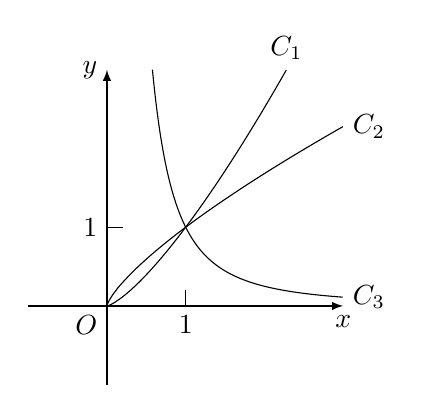
\begin{tikzpicture}[>=latex]
        \draw [->] (-1,0) -- (3,0) node [below] {$x$};
        \draw [->] (0,-1) -- (0,3) node [left] {$y$};
        \draw (0,0) node [below left] {$O$};
        \draw (1,0.2) -- (1,0) node [below] {$1$};
        \draw (0.2,1) -- (0,1) node [left] {$1$};
        \draw [domain = {sqrt(3)/3}:3, samples = 400] plot (\x,{\x^(-2)});
        \draw [domain = 0:3, samples = 400] plot (\x,{\x^(3/4)});
        \draw [domain = 0:{3^(3/4)}, samples = 400] plot (\x,{\x^(4/3)});
        \draw (3,{1/9}) node [right] {$C_3$} (3,{3^(3/4)}) node [right] {$C_2$} ({3^(3/4)},3) node [above] {$C_1$};
    \end{tikzpicture}
\end{center}
\fourch{$\dfrac 43,-2,\dfrac 34$}{$-2,\dfrac 34,\dfrac 43$}{$-2,\dfrac 43,\dfrac 34$}{$\dfrac 34,\dfrac 43,-2$}


关联目标:

暂未关联目标



标签: 第二单元

答案: 暂无答案

解答或提示: 暂无解答与提示

使用记录:

暂无使用记录


出处: 代数精编第三章函数
\item { (005460)}若幂函数$y=x^n$的图像在$0<x<1$时位于直线$y=x$的下方, 则$n$的取值范围是\blank{50}.


关联目标:

暂未关联目标



标签: 第二单元

答案: 暂无答案

解答或提示: 暂无解答与提示

使用记录:

暂无使用记录


出处: 代数精编第三章函数
\item { (005461)}若幂函数$y=x^n$的图像在$0<x<1$时位于直线$y=x$的上方, 则$n$的取值范围是\blank{50}.


关联目标:

暂未关联目标



标签: 第二单元

答案: 暂无答案

解答或提示: 暂无解答与提示

使用记录:

暂无使用记录


出处: 代数精编第三章函数
\item { (005463)}幂函数$y=x^p$与$y=x^q$的图像都通过定点\blank{50}, 它们在第一象限部分关于直线$y=x$对称, 则$p,q$应满足的条件是\blank{50}.


关联目标:

暂未关联目标



标签: 第二单元

答案: 暂无答案

解答或提示: 暂无解答与提示

使用记录:

暂无使用记录


出处: 代数精编第三章函数
\item { (005464)}若实数$a$满足$2.4^a>2.5^a$, 求$a$的取值范围.


关联目标:

暂未关联目标



标签: 第二单元

答案: 暂无答案

解答或提示: 暂无解答与提示

使用记录:

暂无使用记录


出处: 代数精编第三章函数
\item { (005544)}若幂函数$f(x)$是奇函数, 则$f^{-1}(1)=$\blank{50}, $f^{-1}(-1)=$\blank{50}.


关联目标:

暂未关联目标



标签: 第二单元

答案: 暂无答案

解答或提示: 暂无解答与提示

使用记录:

暂无使用记录


出处: 代数精编第三章函数
\item { (005560)}求函数$y=9^x-m\cdot 3^x+1$的最小值.


关联目标:

暂未关联目标



标签: 第二单元

答案: 暂无答案

解答或提示: 令$t=3^x$则函数为$y=t^2-mt+1=(t-\dfrac m2)^2+1-\dfrac{m^2}4$, 其图像的对称轴方程为$t=\dfrac m2$.
(1) 如下图左, 若$\dfrac m2>0$, 则当$t=\dfrac m2$时, $y_{\min }=1-\dfrac{m^2}4$.
\begin{center}
    \begin{tikzpicture}[>=latex]
        \draw [->] (-1,0) -- (3,0) node [below] {$t$};
        \draw [->] (0,-1) -- (0,3) node [left] {$y$};
        \draw (0,0) node [below left] {$O$};
        \draw [dashed, domain = -0.5:0, samples = 100] plot (\x,{(\x-1)^2/2+1});
        \draw [domain = 0:2.5, samples = 100] plot (\x,{(\x-1)^2/2+1});
        \draw [dashed] (1,-0.5) -- (1,2.5);
        \draw (1,0) node [below right] {$\frac{m}{2}$};
        \filldraw [white] (0,1.5) circle (0.05);
        \draw (0,1.5) circle (0.05);
    \end{tikzpicture}
    \begin{tikzpicture}[>=latex]
        \draw [->] (-3,0) -- (1,0) node [below] {$t$};
        \draw [->] (0,-1) -- (0,3) node [left] {$y$};
        \draw (0,0) node [below left] {$O$};
        \draw [dashed, domain = -2.5:0, samples = 100] plot (\x,{(\x+1)^2/2+1});
        \draw [domain = 0:0.5, samples = 100] plot (\x,{(\x+1)^2/2+1});
        \draw [dashed] (-1,-0.5) -- (-1,2.5);
        \draw (-1,0) node [below right] {$\frac{m}{2}$};
        \filldraw [white] (0,1.5) circle (0.05);
        \draw (0,1.5) circle (0.05);
    \end{tikzpicture}
\end{center}
(2) 如上图右, 若$\dfrac m2\le 0$, 则由于$t>0$, 函数无最小值.

使用记录:

暂无使用记录


出处: 代数精编第三章函数
\item { (005561)}填写下表:
\begin{center}
    \begin{tabular}{|c|c|c|c|c|}
        \hline
        $x$	 & $f(x)=x^2$ & $f(x)-f(x-1)$ & $g(x)=2^x$ & $g(x)-g(x-1)$ \\ \hline
        $0$ & & & & \\ \hline
        $1$ & & & & \\ \hline
        $2$ & & & & \\ \hline
        $3$ & & & & \\ \hline
        $4$ & & & & \\ \hline
        $5$ & & & & \\ \hline
        $6$ & & & & \\ \hline
        $7$ & & & & \\ \hline
        $8$ & & & & \\ \hline
        $9$ & & & & \\ \hline
        $10$ & & & & \\ \hline
    \end{tabular}
\end{center}
(1) 比较$f(x)=x^2$与$g(x)=2^x$的函数值的大小;\\
(2) 比较$f(x)=x^2$与$g(x)=2^x$的函数值递增的快慢.


关联目标:

暂未关联目标



标签: 第二单元

答案: 暂无答案

解答或提示: 经计算得下表:
\begin{center}
    \begin{tabular}{|c|c|c|c|c|}
        \hline
        $x$	 & $f(x)=x^2$ & $f(x)-f(x-1)$ & $g(x)=2^x$ & $g(x)-g(x-1)$ \\ \hline
        $0$ & $0$ &  & $1$ & \\ \hline 
        $1$ & $1$ & $1$ & $2$ & $1$ \\  \hline 
        $2$ & $2$ & $1$ & $4$ & $2$\\  \hline 
        $3$ & $9$ & $7$ & $8$ & $4$\\  \hline 
        $4$ & $16$ & $7$ & $16$ & $8$\\  \hline 
        $5$ & $25$ & $9$ & $32$ & $16$\\ \hline 
        $6$ & $36$ & $11$ & $64$ & $32$\\  \hline 
        $7$ & $49$ & $13$ & $128$ & $64$\\ \hline
        $8$ & $64$ & $15$ & $256$ & $128$\\  \hline 
        $9$ & $81$ & $17$ & $512$ & $256$\\  \hline 
        $10$ & $100$ & $19$ & $1024$ & $512$\\ \hline
    \end{tabular}
\end{center}
并描点得出函数$f(x)=x^2$与$g(x)=2^x$在同一个平面直角坐标系下的图像如图所示.
\begin{center}
    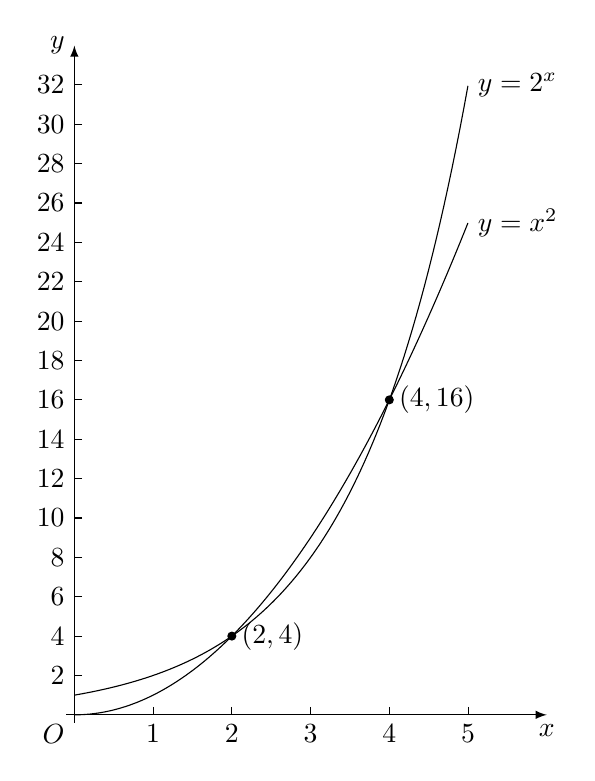
\begin{tikzpicture}[>=latex]
        \draw [->] (-0.1,0) -- (6,0) node [below] {$x$};
        \draw [->] (0,-0.1) -- (0,8.5) node [left] {$y$};
        \draw (0,0) node [below left] {$O$};
        \draw [domain = 0:5,samples = 100] plot (\x,{\x^2/4});
        \draw [domain = 0:5, samples = 100] plot (\x,{2^(\x)/4});
        \draw (5,{25/4}) node [right] {$y=x^2$} (5,8) node [right] {$y=2^x$};
        \filldraw (2,1) circle (0.05) node [right] {$(2,4)$} (4,4) circle (0.05) node [right] {$(4,16)$};
        \foreach \i in {1,2,...,5}{\draw (\i,0.1) -- (\i,0) node [below] {$\i$};};
        \foreach \i in {2,4,...,32}{\draw (0.1,\i/4) -- (0,\i/4) node [left] {$\i$};};
    \end{tikzpicture}
\end{center}
由表和图知:\\
(1) 当$0<x<2$时, $g(x)>f(x)$; 当$2<x<4$时, $f(x)>g(x)$; 当$x>4$时, $g(x)>f(x)$; 当$x=2$或$x=4$时, $f(x)=f(x)$.
(2) 当$x>4$时, $f(x)=x^2$的函数值递增的速度较$g(x)=2^x$慢.

使用记录:

暂无使用记录


出处: 代数精编第三章函数
\item { (005562)}已知函数$f(x)=2x+1$, $g(x)=1.5^x$, $h(x)=x^{1.5}$, 试用数值计算比较三个函数在$[0,+\infty)$上的函数值的大小、图像递增的快慢. 并说明在函数图像上的表现.
解  列表并计算得:
\begin{center}
    \begin{longtable}{|c|c|c|c|c|c|c|}
        \hline
        $x$	 & $f(x)=2x+1$ & $f(x)-f(x-1)$ & $g(x)=1.5^x$ & $g(x)-g(x-1)$ & $h(x)=x^{1.5}$ & $h(x)-h(x-1)$ \\ \hline
        \endhead
        $0$ & $1$ & & $1$ & & $0$ &  \\ \hline
        $1$ & $3$ & $2$ & $1.5$ & $0.5$ & $1$ & $1$\\ \hline
        $2$ & $5$ & $2$ & $2.25$ & $0.75$ & $2.82842712$ & $1.82842712$\\ \hline
        $3$ & $7$ & $2$ & $3.375$ & $1.125$ & $5.19615242$ & $2.3677253$\\ \hline
        $4$ & $9$ & $2$ & $5.0625$ & $1.6875$ & $8$ & $2.80384758$\\ \hline
        $5$ & $11$ & $2$ & $7.59375$ & $2.53125$ & $11.1803399$ & $3.18033989$\\ \hline
        $6$ & $13$ & $2$ & $11.390625$ & $3.796875$ & $14.6969385$ & $3.51659857$\\ \hline
        $7$ & $15$ & $2$ & $17.085938$ & $5.6953125$ & $18.5202592$ & $3.82332072$\\ \hline
        $8$ & $17$ & $2$ & $25.628906$ & $8.5429688$ & $22.627417$ & $4.10715782$\\ \hline
        $9$ & $19$ & $2$ & $38.443359$ & $12.814453$ & $27$ & $4.372583$\\ \hline
        $10$ & $21$ & $2$ & $57.665039$ & $19.22168$ & $31.6227766$ & $4.6227766$\\ \hline
        $11$ & $23$ & $2$ & $86.497559$ & $28.83252$ & $36.4828727$ & $4.86009609$\\ \hline
        $12$ & $25$ & $2$ & $129.74634$ & $43.248779$ & $41.5692194$ & $5.08634669$\\ \hline
        $13$ & $27$ & $2$ & $194.61951$ & $64.873169$ & $46.8721666$ & $5.3029472$\\ \hline
        $14$ & $29$ & $2$ & $291.92926$ & $97.309753$ & $52.3832034$ & $5.51103683$\\ \hline
        $15$ & $31$ & $2$ & $437.89389$ & $145.96463$ & $58.0947502$ & $5.71154678$\\ \hline
        $16$ & $33$ & $2$ & $656.84084$ & $218.94695$ & $64$ & $5.90524981$\\ \hline
        $17$ & $35$ & $2$ & $985.26125$ & $328.42042$ & $70.0927956$ & $6.09279564$\\ \hline
        $18$ & $37$ & $2$ & $1477.8919$ & $492.63063$ & $76.3675324$ & $6.27473673$\\ \hline
        $19$ & $39$ & $2$ & $2216.8378$ & $738.94594$ & $82.8190799$ & $6.45154756$\\ \hline
        $20$ & $41$ & $2$ & $3325.2567$ & $1108.4189$ & $89.4427191$ & $6.62363917$\\ \hline
        $21$ & $43$ & $2$ & $4987.8851$ & $1662.6284$ & $96.2340896$ & $6.79137049$\\ \hline
        $22$ & $45$ & $2$ & $7481.8276$ & $2493.9425$ & $103.189147$ & $6.95505712$\\ \hline
        $23$ & $47$ & $2$ & $11222.741$ & $3740.9138$ & $110.304125$ & $7.11497832$\\ \hline
        $24$ & $49$ & $2$ & $16834.112$ & $5611.3707$ & $117.575508$ & $7.27138262$\\ \hline
        $25$ & $51$ & $2$ & $25251.168$ & $8417.0561$ & $125$ & $7.42449235$\\ \hline
        $26$ & $53$ & $2$ & $37876.752$ & $12625.584$ & $132.574507$ & $7.57450735$\\ \hline
        $27$ & $55$ & $2$ & $56815.129$ & $18938.376$ & $140.296115$ & $7.72160806$\\ \hline
        $28$ & $57$ & $2$ & $85222.693$ & $28407.564$ & $148.162073$ & $7.86595801$\\ \hline
        $29$ & $59$ & $2$ & $127834.04$ & $42611.346$ & $156.169779$ & $8.00770599$\\ \hline
        $30$ & $61$ & $2$ & $191751.06$ & $63917.02$ & $164.316767$ & $8.14698784$\\ \hline
        $\cdots$ & $\cdots$ & $\cdots$ & $\cdots$ & $\cdots$ & $\cdots$ & $\cdots$ \\ \hline
    \end{longtable}
\end{center}
得点$A,B,C,D$的横坐标分别约为$1.5,4.8, 6.5, 7.4$, 记作$x_A,x_B,x_C,x_D$.\\
(1) 三个函数的函数值的大小情况如下:\\
\textcircled{1} 当$0<x<x_A$时, $f(x)>g(x)>h(x)$;
\textcircled{2} 当$x_A<x<x_B$时, $f(x)>h(x)>g(x)$;
\textcircled{3} 由$x_B<x<x_C$时, $h(x)>f(x)>g(x)$;
\textcircled{4} 当$x_C<x<x_D$时, $h(x)>g(x)>f(x)$;
\textcircled{5} 当$x_D<x$时, $g(x)>h(x)>f(x)$;
\textcircled{6} 当$x=x_A$时, $f(x)>g(x)=h(x)$;
\textcircled{7} 当$x=x_B$时, $f(x)=h(x)>g(x)$;
\textcircled{8} 当$x=x_C$时, $f(x)=g(x)<h(x)$;
\textcircled{9} 当$x=x_D$时, $f(x)<g(x)=g(x)$.\\
(2) 它们在同一个平面直角坐标系下的图像如图14所示.
\begin{center}
    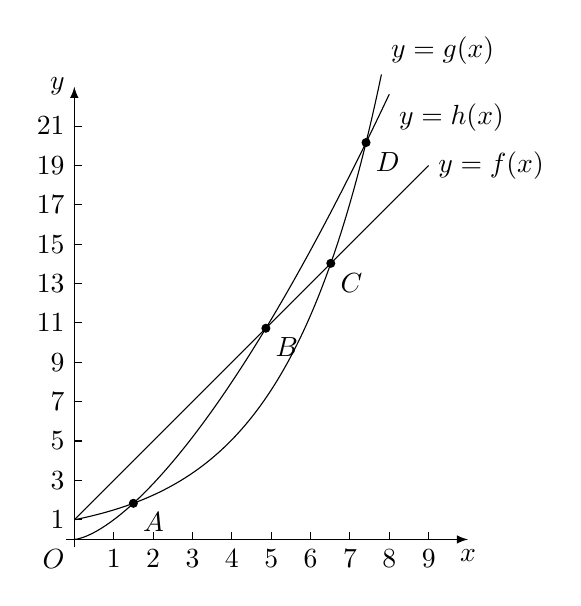
\begin{tikzpicture}[>=latex]
        \draw [->] (-0.1,0) -- (5,0) node [below] {$x$};
        \draw [->] (0,-0.1) -- (0,5.75) node [left] {$y$};
        \draw (0,0) node [below left] {$O$};
        \draw [domain = 0:9,samples = 100, name path = firstorder] plot ({\x/2},{(2*\x+1)/4});
        \draw (4.5,{19/4}) node [right] {$y=f(x)$};
        \draw [domain = 0:7.8, samples = 100, name path = exponential] plot ({\x/2},{1.5^(\x)/4}); 
        \draw (3.9,{1.5^7.8/4}) node [above right] {$y=g(x)$};
        \draw [domain = 0:8, samples = 100, name path = power] plot ({\x/2},{\x^(3/2)/4});
        \draw (4,{8^(3/2)/4}) node [below right] {$y=h(x)$};
        \path [name intersections = {of = firstorder and exponential, by = {T,C}}];
        \path [name intersections = {of = firstorder and power, by = B}];
        \path [name intersections = {of = exponential and power, by = {A,D}}];
        \filldraw (A) circle (0.05) node [below right] {$A$};
        \filldraw (B) circle (0.05) node [below right] {$B$};
        \filldraw (C) circle (0.05) node [below right] {$C$};
        \filldraw (D) circle (0.05) node [below right] {$D$};
        \foreach \i in {1,2,...,9}{\draw (\i/2,0.1) -- (\i/2,0) node [below] {$\i$};};
        \foreach \i in {1,3,...,21}{\draw (0.1,\i/4) -- (0,\i/4) node [left] {$\i$};};
    \end{tikzpicture}
\end{center}
由表格及图像可看出, 三个函数的函数值变化及相应增量规律为: 随着$x$的增大, 直线型均匀上升, 增量恒定; 指数型急剧上升, 在区间$[0,+\infty)$上递增增量快速增大; 幂函数型虽上升较快, 但随着$x$的不断增大上升趋势远不如指数型, 几乎微不足道, 其增量缓慢递增.


关联目标:

暂未关联目标



标签: 第二单元

答案: 暂无答案

解答或提示: 暂无解答与提示

使用记录:

暂无使用记录


出处: 代数精编第三章函数
\item { (005564)}下列函数中, 值域为$(0,+\infty)$的函数是\bracket{20}.
\fourch{$y=(\dfrac 18)^{2-x}$}{$y=\sqrt {1-3^x}$}{$y=\sqrt {(\dfrac 13)^x-1}$}{$y=2^{\frac 1{3-x}}$}


关联目标:

暂未关联目标



标签: 第二单元

答案: 暂无答案

解答或提示: 暂无解答与提示

使用记录:

暂无使用记录


出处: 代数精编第三章函数
\item { (005566)}下列函数式中, 满足$f(x+1)=2f(x)$的$f(x)$是\bracket{20}.
\fourch{$\dfrac 12(x+1)$}{$x+\dfrac 14$}{$2^x$}{$2^{-x}$}


关联目标:

暂未关联目标



标签: 第二单元

答案: 暂无答案

解答或提示: 暂无解答与提示

使用记录:

暂无使用记录


出处: 代数精编第三章函数
\item { (005567)}若$f(x)=\dfrac{\mathrm{e}^x-\mathrm{e}^{-x}}2$, $g(x)=\dfrac{\mathrm{e}^x+\mathrm{e}^{-x}}2$.则下列关系式中不正确的是\bracket{20}.
\twoch{$[g(x)]^2-[f(x)]^2=1$}{$f(2x)=2f(x)\cdot g(x)$}{$g(2x)=[f(x)]^2+[g(x)]^2$}{$f(-x)g(x)=f(x)g(-x)$}


关联目标:

暂未关联目标



标签: 第二单元

答案: 暂无答案

解答或提示: 暂无解答与提示

使用记录:

暂无使用记录


出处: 代数精编第三章函数
\item { (005568)}若$a>b$且$ab\ne 0$.则在\textcircled{1} $a^2>b^2$, \textcircled{2} $2^a>2^b$, \textcircled{3} $\dfrac 1a<\dfrac 1b$, \textcircled{4} $a^{\frac 13}>b^{\frac 13}$, \textcircled{5} $(\dfrac 13)^a<(\dfrac 13)^b$这五个关系式中, 恒成立的有\bracket{20}.
\fourch{$1$个}{$2$个}{$3$个}{$4$个}


关联目标:

暂未关联目标



标签: 第二单元

答案: 暂无答案

解答或提示: 暂无解答与提示

使用记录:

暂无使用记录


出处: 代数精编第三章函数
\item { (005569)}在同一平面直角坐标系中, 函数$f(x)=ax$与$g(x)=a^x$的图像可能是\bracket{20}.
\fourch{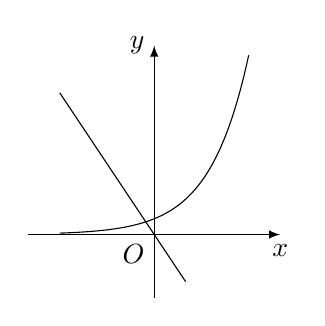
\begin{tikzpicture}[scale = 0.2, >=latex]
    \draw [->] (-8,0) -- (8,0) node [below] {$x$};
    \draw [->] (0,-4) -- (0,12) node [left] {$y$};
    \draw (0,0) node [below left] {$O$};
    \draw [domain = -6:2, samples = 100] plot (\x,{-1.5*\x});
    \draw [domain = -6:6, samples = 100] plot (\x,{1.5^\x});
\end{tikzpicture}}{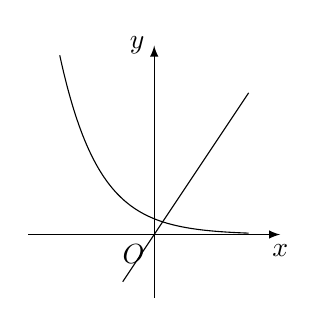
\begin{tikzpicture}[scale = 0.2, >=latex]
    \draw [->] (-8,0) -- (8,0) node [below] {$x$};
    \draw [->] (0,-4) -- (0,12) node [left] {$y$};
    \draw (0,0) node [below left] {$O$};
    \draw [domain = -2:6, samples = 100] plot (\x,{1.5*\x});
    \draw [domain = -6:6, samples = 100] plot (-\x,{1.5^\x});
\end{tikzpicture}}{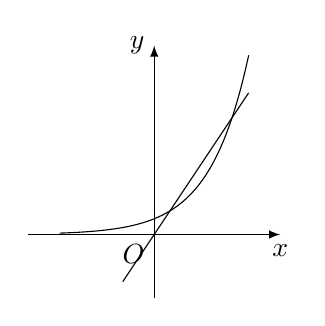
\begin{tikzpicture}[scale = 0.2, >=latex]
    \draw [->] (-8,0) -- (8,0) node [below] {$x$};
    \draw [->] (0,-4) -- (0,12) node [left] {$y$};
    \draw (0,0) node [below left] {$O$};
    \draw [domain = -2:6, samples = 100] plot (\x,{1.5*\x});
    \draw [domain = -6:6, samples = 100] plot (\x,{1.5^\x});
\end{tikzpicture}}{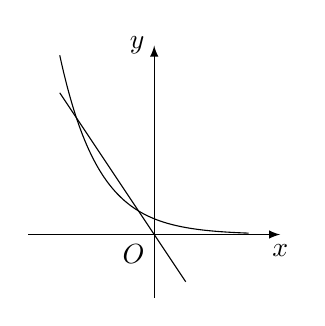
\begin{tikzpicture}[scale = 0.2, >=latex]
    \draw [->] (-8,0) -- (8,0) node [below] {$x$};
    \draw [->] (0,-4) -- (0,12) node [left] {$y$};
    \draw (0,0) node [below left] {$O$};
    \draw [domain = -2:6, samples = 100] plot (-\x,{1.5*\x});
    \draw [domain = -6:6, samples = 100] plot (-\x,{1.5^\x});
\end{tikzpicture}}


关联目标:

暂未关联目标



标签: 第二单元

答案: 暂无答案

解答或提示: 暂无解答与提示

使用记录:

暂无使用记录


出处: 代数精编第三章函数
\item { (005571)}若$f(x)$在$(0,+\infty)$上是减函数, 而$f(a^x)$在$(-\infty ,+\infty)$上是增函数, 则实数$a$的取值范围是\bracket{20}.
\fourch{(0, 1)}{$(0,1)\cup (1,+\infty)$}{$(0,+\infty)$}{$(1,+\infty)$}


关联目标:

暂未关联目标



标签: 第二单元

答案: 暂无答案

解答或提示: 暂无解答与提示

使用记录:

暂无使用记录


出处: 代数精编第三章函数
\item { (005573)}若函数$f(x)=(a^2-1)^x$在$(-\infty ,+\infty)$上是减函数, 则$a$的取值范围是\bracket{20}.
\fourch{$|a|>1$}{$|a|<\sqrt 2$}{$a>\sqrt 2$}{$1<|a|<\sqrt 2$}


关联目标:

暂未关联目标



标签: 第二单元

答案: 暂无答案

解答或提示: 暂无解答与提示

使用记录:

暂无使用记录


出处: 代数精编第三章函数
\item { (005574)}若函数$f(x)=a^x-(b+1)$($a>0$且$a\ne 1$)的图像在第一、三、四象限, 则必有\bracket{20}.
\fourch{$0<a<1$且$b>0$}{$0<a<1$且$b<0$}{$a>1$且$b<1$}{$a>1$且$b>0$}


关联目标:

暂未关联目标



标签: 第二单元

答案: 暂无答案

解答或提示: 暂无解答与提示

使用记录:

暂无使用记录


出处: 代数精编第三章函数
\item { (005577)}根据条件确定实数$x$的取值范围:\\
(1) $2^x>0.5$:\blank{50};\\
(2) $2^x<1$:\blank{50};\\
(3) $0.2^{2x-1}>\dfrac 1{25}$:\blank{50};\\
(4) $8<(\dfrac 12)^{2x+1}$:\blank{50};\\
(5) $(a^2+a+2)^x>(a^2+a+2)^{1-x}$:\blank{50};\\
(6) $(\dfrac 12)^{x^2+x-2}<1$:\blank{50}.


关联目标:

暂未关联目标



标签: 第二单元

答案: 暂无答案

解答或提示: 暂无解答与提示

使用记录:

暂无使用记录


出处: 代数精编第三章函数
\item { (005579)}若函数$f(x)$的定义域是$(0, 1)$, 则函数$f(2^{-x})$的定义域是\blank{50}, $f(3\times 9^x+2\times 3^x)$的定义域是\blank{50}.


关联目标:

暂未关联目标



标签: 第二单元

答案: 暂无答案

解答或提示: 暂无解答与提示

使用记录:

暂无使用记录


出处: 代数精编第三章函数
\item { (005586)}函数$f(x)=a^{2x}-3a^x+2$($a>0$且$a\ne 1$)的最小值为\blank{50}.


关联目标:

暂未关联目标



标签: 第二单元

答案: 暂无答案

解答或提示: 暂无解答与提示

使用记录:

暂无使用记录


出处: 代数精编第三章函数
\item { (005588)}函数$f(x)=\dfrac 1{3^x-1}$的值域是\blank{50}.


关联目标:

暂未关联目标



标签: 第二单元

答案: 暂无答案

解答或提示: 暂无解答与提示

使用记录:

暂无使用记录


出处: 代数精编第三章函数
\item { (005589)}函数$f(x)=\dfrac{3^x}{3^x+1}$的值域是\blank{50}.


关联目标:

暂未关联目标



标签: 第二单元

答案: 暂无答案

解答或提示: 暂无解答与提示

使用记录:

暂无使用记录


出处: 代数精编第三章函数
\item { (005590)}若关于$x$的方程$5^x=\dfrac{a+3}{5-a}$有负根, 则实数$a$的取值范围是\blank{50}.


关联目标:

暂未关联目标



标签: 第二单元

答案: 暂无答案

解答或提示: 暂无解答与提示

使用记录:

暂无使用记录


出处: 代数精编第三章函数
\item { (005591)}若$0<a<1$, $x>y>1$, 则$a^x$, $x^a$, $a^y$, $y^a$从小到大的排列顺序是\blank{50}.


关联目标:

暂未关联目标



标签: 第二单元

答案: 暂无答案

解答或提示: 暂无解答与提示

使用记录:

暂无使用记录


出处: 代数精编第三章函数
\item { (005592)}若$0.9<a<1$, 则$a$, $a^a$, $a^{a^a}$从小到大的排列顺序是\blank{50}.


关联目标:

暂未关联目标



标签: 第二单元

答案: 暂无答案

解答或提示: 暂无解答与提示

使用记录:

暂无使用记录


出处: 代数精编第三章函数
\item { (005594)}若$f(x)=a+\dfrac 1{4^x+1}$是奇函数, 求常数$a$的值.


关联目标:

暂未关联目标



标签: 第二单元

答案: 暂无答案

解答或提示: 暂无解答与提示

使用记录:

暂无使用记录


出处: 代数精编第三章函数
\item { (005595)}若$f(x)=x^2(\dfrac 1{a^x-1}+m)$($a>0$且$a\ne 1$)为奇函数, 求常数$m$的值.


关联目标:

暂未关联目标



标签: 第二单元

答案: 暂无答案

解答或提示: 暂无解答与提示

使用记录:

暂无使用记录


出处: 代数精编第三章函数
\item { (005596)}已知函数$f(x)=(\dfrac 1{2^x-1}+\dfrac 12)x^3$.\\
(1) 求函数的定义域;\\
(2) 讨论$f(x)$的奇偶性;\\
(3) 求证: $f(x)>0$.


关联目标:

暂未关联目标



标签: 第二单元

答案: 暂无答案

解答或提示: 暂无解答与提示

使用记录:

暂无使用记录


出处: 代数精编第三章函数
\item { (005597)}已知$f(x)=\dfrac{a^x-1}{a^x+1}$($a>1$).\\
(1) 判断函数$f(x)$的奇偶性;\\
(2) 求函数$f(x)$的值域;\\
(3) 求证: $f(x)$在区间$(-\infty ,+\infty)$上是增函数.


关联目标:

暂未关联目标



标签: 第二单元

答案: 暂无答案

解答或提示: 暂无解答与提示

使用记录:

暂无使用记录


出处: 代数精编第三章函数
\item { (005598)}若$0\le x\le 2$, 求函数$y=4^{x-\frac 12}-3\cdot 2^x+5$的最大值和最小值.


关联目标:

暂未关联目标



标签: 第二单元

答案: 暂无答案

解答或提示: 暂无解答与提示

使用记录:

暂无使用记录


出处: 代数精编第三章函数
\item { (005599)}若函数$f(x)=a^{2x}+2a^x-1$($a>0$且$a\ne 1$)在$[-1, 1]$上的最大值为$14$, 求实数$a$的值.


关联目标:

暂未关联目标



标签: 第二单元

答案: 暂无答案

解答或提示: 暂无解答与提示

使用记录:

暂无使用记录


出处: 代数精编第三章函数
\item { (005600)}已知函数$f(x)=\dfrac a{a^2-2}(a^x-a^{-x})$($a>0$且$a\ne 1$)在$(-\infty ,+\infty)$上是增函数, 求实数$a$的取值范围.


关联目标:

暂未关联目标



标签: 第二单元

答案: 暂无答案

解答或提示: 暂无解答与提示

使用记录:

暂无使用记录


出处: 代数精编第三章函数
\item { (005602)}已知集合$M=\{x|(x+1)^2\le 1\}$, $P=\{y|y=4^x-a\cdot 2^{x+1}+1,\ x\in M,\ \dfrac 34<a\le 1\}$, 且全集$U=\mathbf{R}$, 求$\complement _U(M\cup P)$.


关联目标:

暂未关联目标



标签: 第二单元

答案: 暂无答案

解答或提示: 暂无解答与提示

使用记录:

暂无使用记录


出处: 代数精编第三章函数
\item { (005603)}求方程$x^{\frac 13}+2^x=0$的实根个数.


关联目标:

暂未关联目标



标签: 第二单元

答案: 暂无答案

解答或提示: 暂无解答与提示

使用记录:

暂无使用记录


出处: 代数精编第三章函数
\item { (005604)}求关于$x$的方程$a^x+1=-x^2+2x+2a$($a>0$且$a\ne 1$)的实数解的个数.


关联目标:

暂未关联目标



标签: 第二单元

答案: 暂无答案

解答或提示: 暂无解答与提示

使用记录:

暂无使用记录


出处: 代数精编第三章函数
\item { (005605)}在同一个平面直角坐标系中, 作出$t(x)=0.5x$与$g(x)=0.2\times 2^x$的图像, 并比较它们的增长情况.


关联目标:

暂未关联目标



标签: 第二单元

答案: 暂无答案

解答或提示: 暂无解答与提示

使用记录:

暂无使用记录


出处: 代数精编第三章函数
\item { (005606)}某地区不同身高的未成年男性的体重平均值如下表(身高: $\text{cm}$; 体重: $\text{kg}$):
\begin{center}
    \begin{tabular}{|c|c|c|c|c|c|c|}
        \hline
        身高 & $60$ & $70$ & $80$ & $90$ & $100$ & $110$\\ \hline
        体重 & $6.13$ & $7.90$ & $9.99$ & $12.15$ & $15.02$ & $17.05$\\ \hline
        身高 & $120$ & $130$ & $140$ & $150$ & $160$ & $170$\\ \hline
        体重 & $20.92$ & $26.86$ & $31.11$ & $38.85$ & $47.25$ & $55.05$\\ \hline
    \end{tabular}
\end{center}
为了揭示未成年男性的身高与体重的规律, 甲选择了模型$y=ax^2+bx+c$($a>0$), 乙选择了模型$y=ba^x$($a>1$), 其中$y$表示体重, $x$表示身高.你认为谁选择的模型较好?


关联目标:

暂未关联目标



标签: 第二单元

答案: 暂无答案

解答或提示: 暂无解答与提示

使用记录:

暂无使用记录


出处: 代数精编第三章函数
\item { (005607)}用计算器计算并填写下表:
\begin{center}
    \begin{tabular}{|c|c|c|c|c|}
        \hline
        $x$	& $f(x)=x^{\frac 12}$ & $g(x)=x^{0.6}$ & $h(x)=2.1^x$ & $s(x)=2.2^x$ \\ \hline
        $0$ & & & & \\ \hline
        $1$ & & & & \\ \hline
        $2$ & & & & \\ \hline
        $3$ & & & & \\ \hline
        $4$ & & & & \\ \hline
        $5$ & & & & \\ \hline
        $6$ & & & & \\ \hline
        $7$ & & & & \\ \hline
        $8$ & & & & \\ \hline
        $9$ & & & & \\ \hline
        $10$ & & & & \\ \hline
    \end{tabular}
\end{center}
从表中变化的现象可以归纳出哪些函数递增的规律?\\
(1) 幂函数$f(x)$与$g(x)$之间比较得出的规律;
(2) 指数函数$h(x)$与$s(x)$之间比较得出的规律;
(3) 幂函数$f(x)=x^{\frac 12}$与指数函数$h(x)$之间比较得出的规律


关联目标:

暂未关联目标



标签: 第二单元

答案: 暂无答案

解答或提示: 暂无解答与提示

使用记录:

暂无使用记录


出处: 代数精编第三章函数
\item { (005608)}求$\log_927$的值.


关联目标:

暂未关联目标



标签: 第二单元

答案: 暂无答案

解答或提示: 设$\log_927=x$, 根据对数的定义有$9^x=27$.即$3^{2x}=3^3$,
所以$ 2x=3,x=\dfrac 32$, 即$\log_927=\dfrac 32$.
注意  $\log_aN$的定义至关重要, 它始终是解对数问题的首要手段.根据定义, 显然有$\log_a1=0$, $\log_aa=1$, $\log_aa^m=m$, $a^{\log_aN}=N$($a>0$且$a\ne 1$, $N>0$).
学习了换底公式后, 本例还可按以下方法求值:
$\log_927=\dfrac{\log_327}{\log_39}=\dfrac{3\log_33}{2\log_33}=\dfrac 32$, 或$\log_927=\log_{3^2}3^3=\dfrac 32\log_33=\dfrac 32$.

使用记录:

暂无使用记录


出处: 代数精编第三章函数
\item { (005609)}设$3^a=4^b=36$, 求$\dfrac 2a+\dfrac 1b$的值.


关联目标:

暂未关联目标



标签: 第二单元

答案: 暂无答案

解答或提示: 对已知条件取以6为底的对数, 得
$\dfrac 2a=\log_63$, $\dfrac 1b=\log_62$, 于是$\dfrac 2a+\dfrac 1b=\log_63+\log_62=\log_66=1$.

使用记录:

暂无使用记录


出处: 代数精编第三章函数
\item { (005610)}已知$x=a^{\frac 1{1-\log_ay}}$, $y=a^{\frac 1{1-\log_az}}$求证: $z=a^{\frac 1{1-\log_ax}}$.


关联目标:

暂未关联目标



标签: 第二单元

答案: 暂无答案

解答或提示: 由$x=a^{\frac 1{1-\log_ay}}$, 得$\log_ax=\dfrac 1{1-\log_ay}$.
同理$\log_ay=\dfrac 1{1-\log_az}$, 代入上式, 消去$\log_ay$,
得$\log_ax=\dfrac 1{1-\dfrac 1{1-\log_az}}=\dfrac{1-\log_az}{-\log_az}$, 即$\log_az=\dfrac 1{1-\log_ax}$, 所以$ z=a^{\frac 1{1-\log_ax}}$.

使用记录:

暂无使用记录


出处: 代数精编第三章函数
\item { (005611)}已知$\log_{12}27=a$, 求$\log_616$.


关联目标:

暂未关联目标



标签: 第二单元

答案: 暂无答案

解答或提示: 由已知, 得$a=\log_{12}27=\dfrac{\log_327}{\log_312}=\dfrac 3{1+2\log_32}$, 所以$ \log_32=\dfrac{3-a}{2a}$.
于是$\log_616=\dfrac{\log_316}{\log_36}=\dfrac{4\log_32}{1+\log_32}=\dfrac{4(3-a)}{3+a}$.

使用记录:

暂无使用记录


出处: 代数精编第三章函数
\item { (005612)}若$a=b^2$($b>0$, $b\ne 1$), 则有\bracket{20}.
\fourch{$\log_2a=b$}{$\log_2b=a$}{$\log_ab=2$}{$\log_ba=2$}


关联目标:

暂未关联目标



标签: 第二单元

答案: 暂无答案

解答或提示: 暂无解答与提示

使用记录:

暂无使用记录


出处: 代数精编第三章函数
\item { (005613)}若$\log_x\sqrt[7]y=z$, 则$x,y,z$之间满足\bracket{20}.
\fourch{$y^7=x^z$}{$y=x^{7z}$}{$y=7x^z$}{$y=z^{7x}$}


关联目标:

暂未关联目标



标签: 第二单元

答案: 暂无答案

解答或提示: 暂无解答与提示

使用记录:

暂无使用记录


出处: 代数精编第三章函数
\item { (005614)}$2^{\log_43}$的值等于\bracket{20}.
\fourch{3}{$\sqrt 3$}{$\dfrac{\sqrt 3}3$}{$\dfrac 13$}


关联目标:

暂未关联目标



标签: 第二单元

答案: 暂无答案

解答或提示: 暂无解答与提示

使用记录:

暂无使用记录


出处: 代数精编第三章函数
\item { (005615)}$\log_ab\cdot \log_3a=5$, 则$b=$\bracket{20}.
\fourch{$a^3$}{$a^5$}{$3^5$}{$5^3$}


关联目标:

暂未关联目标



标签: 第二单元

答案: 暂无答案

解答或提示: 暂无解答与提示

使用记录:

暂无使用记录


出处: 代数精编第三章函数
\item { (005616)}若点$P(\lg a,\lg b)$关于$x$轴的对称点的坐标是(0, -1), 则$a$和$b$的值是\bracket{20}.
\fourch{$a=1$, $b=10$}{$a=1$, $b=\dfrac 1{10}$}{$a=10$, $b=1$}{$a=\dfrac 1{10}$, $b=1$}


关联目标:

暂未关联目标



标签: 第二单元

答案: 暂无答案

解答或提示: 暂无解答与提示

使用记录:

暂无使用记录


出处: 代数精编第三章函数
\item { (005617)}给出下列四个式子(已知$a>0$, $a\ne 1$, $x>y>0$): \textcircled{1} $\log_ax\cdot \log_ay=\log_a(x+y)$; \textcircled{2} $\log_ax+\log_ay=\log_a(x+y)$; \textcircled{3} $\log_a\dfrac xy=\log_a(x-y)$; \textcircled{4} $\log_a(x-y)=\dfrac{\log_ax}{\log_ay}$.其中正确的有\bracket{20}.
\fourch{$0$个}{$1$个}{$2$个}{$3$个}


关联目标:

暂未关联目标



标签: 第二单元

答案: 暂无答案

解答或提示: 暂无解答与提示

使用记录:

暂无使用记录


出处: 代数精编第三章函数
\item { (005618)}若$m>0$, 且$10^x=\lg (10m)+\lg \dfrac 1m$, 则$x$的值为\bracket{20}.
\fourch{$2$}{$1$}{$0$}{$-1$}


关联目标:

暂未关联目标



标签: 第二单元

答案: 暂无答案

解答或提示: 暂无解答与提示

使用记录:

暂无使用记录


出处: 代数精编第三章函数
\item { (005619)}若$\lg x=a$, $\lg y=b$, 则$\lg \sqrt x-\lg (\dfrac y{10})^2$的值等于\bracket{20}.
\fourch{$\dfrac 12a-2b-2$}{$\dfrac 12a-2b+2$}{$\dfrac 12a-2b-1$}{$\dfrac 12a-2b+1$}


关联目标:

暂未关联目标



标签: 第二单元

答案: 暂无答案

解答或提示: 暂无解答与提示

使用记录:

暂无使用记录


出处: 代数精编第三章函数
\item { (005620)}如果方程$\lg ^2x+(\lg 2+\lg 3)\lg x+\lg 2\cdot \lg 3=0$的两个根为$x_1,x_2$, 那么$x_1\cdot x_2$的值为\bracket{20}.
\fourch{$\lg 2\cdot \lg 3$}{$\lg 2+\lg 3$}{$\dfrac 16$}{$-6$}


关联目标:

暂未关联目标



标签: 第二单元

答案: 暂无答案

解答或提示: 暂无解答与提示

使用记录:

暂无使用记录


出处: 代数精编第三章函数
\item { (005621)}若$x=t^{\frac 1{t-1}}$, $y=t^{\frac t{t-1}}$($t>0$, $t\ne 1$), 则$x,y$之间的关系是\bracket{20}.
\fourch{$y^x=x^{\frac 1y}$}{$y^{\frac 1x}=x^y$}{$y^x=x^y$}{$x^x=y^y$}


关联目标:

暂未关联目标



标签: 第二单元

答案: 暂无答案

解答或提示: 暂无解答与提示

使用记录:

暂无使用记录


出处: 代数精编第三章函数
\item { (005622)}若$\log_8x=-\dfrac 23$, 则$x=$\blank{50}.


关联目标:

暂未关联目标



标签: 第二单元

答案: 暂无答案

解答或提示: 暂无解答与提示

使用记录:

暂无使用记录


出处: 代数精编第三章函数
\item { (005623)}若$\log_x27=\dfrac 34$, 则$x=$\blank{50}.


关联目标:

暂未关联目标



标签: 第二单元

答案: 暂无答案

解答或提示: 暂无解答与提示

使用记录:

暂无使用记录


出处: 代数精编第三章函数
\item { (005624)}若$\log_2(\log_5x)=0$, 则$x=$\blank{50}.


关联目标:

暂未关联目标



标签: 第二单元

答案: 暂无答案

解答或提示: 暂无解答与提示

使用记录:

暂无使用记录


出处: 代数精编第三章函数
\item { (005625)}若$\log_2(\lg x)=1$, 则$x=$\blank{50}.


关联目标:

暂未关联目标



标签: 第二单元

答案: 暂无答案

解答或提示: 暂无解答与提示

使用记录:

暂无使用记录


出处: 代数精编第三章函数
\item { (005626)}若$\log_2[\log_3(\log_5x)]=0$, 则$x=$\blank{50}.


关联目标:

暂未关联目标



标签: 第二单元

答案: 暂无答案

解答或提示: 暂无解答与提示

使用记录:

暂无使用记录


出处: 代数精编第三章函数
\item { (005627)}若$\log_2[\log_3(\log_4x)]=\log_3[\log_4(\log_2y)]=\log_4[\log_2(\log_3z)]=0$.则$x+y+z=$\blank{50}.


关联目标:

暂未关联目标



标签: 第二单元

答案: 暂无答案

解答或提示: 暂无解答与提示

使用记录:

暂无使用记录


出处: 代数精编第三章函数
\item { (005628)}计算: $2^{\log_4(2-\sqrt 3)^2}+3^{\log_9(2+\sqrt 3)^2}=$\blank{50}.


关联目标:

暂未关联目标



标签: 第二单元

答案: 暂无答案

解答或提示: 暂无解答与提示

使用记录:

暂无使用记录


出处: 代数精编第三章函数
\item { (005629)}计算: $2^{1+\dfrac 12\log_25}=$\blank{50}.


关联目标:

暂未关联目标



标签: 第二单元

答案: 暂无答案

解答或提示: 暂无解答与提示

使用记录:

暂无使用记录


出处: 代数精编第三章函数
\item { (005630)}计算: $9^{\log_32}=$\blank{50}.


关联目标:

暂未关联目标



标签: 第二单元

答案: 暂无答案

解答或提示: 暂无解答与提示

使用记录:

暂无使用记录


出处: 代数精编第三章函数
\item { (005631)}计算: $5^{3-2\log_{25}125}=$\blank{50}.


关联目标:

暂未关联目标



标签: 第二单元

答案: 暂无答案

解答或提示: 暂无解答与提示

使用记录:

暂无使用记录


出处: 代数精编第三章函数
\item { (005632)}计算: $\log_{(2-\sqrt 3)}(7+4\sqrt 3)=$\blank{50}.


关联目标:

暂未关联目标



标签: 第二单元

答案: 暂无答案

解答或提示: 暂无解答与提示

使用记录:

暂无使用记录


出处: 代数精编第三章函数
\item { (005633)}计算: $\log_6(\sqrt {2+\sqrt 3}+\sqrt {2-\sqrt 3})=$\blank{50}.


关联目标:

暂未关联目标



标签: 第二单元

答案: 暂无答案

解答或提示: 暂无解答与提示

使用记录:

暂无使用记录


出处: 代数精编第三章函数
\item { (005634)}计算: $(2+\sqrt 3)^{-1}-\log_{(2+\sqrt 3)}(7+4\sqrt 3)=$\blank{50}.


关联目标:

暂未关联目标



标签: 第二单元

答案: 暂无答案

解答或提示: 暂无解答与提示

使用记录:

暂无使用记录


出处: 代数精编第三章函数
\item { (005635)}计算: $-2^2\div (-\dfrac{27}8)^{-\frac 13}-(0.7)^{\lg 1}+\log_3\dfrac 14+\log_312=$\blank{50}.


关联目标:

暂未关联目标



标签: 第二单元

答案: 暂无答案

解答或提示: 暂无解答与提示

使用记录:

暂无使用记录


出处: 代数精编第三章函数
\item { (005636)}若$3^x=12^y=8$, 则$\dfrac 1x-\dfrac 1y=$\blank{50}.


关联目标:

暂未关联目标



标签: 第二单元

答案: 暂无答案

解答或提示: 暂无解答与提示

使用记录:

暂无使用记录


出处: 代数精编第三章函数
\item { (005637)}若$2^x=7^y=196$, 则$\dfrac 1x+\dfrac 1y=$\blank{50}.


关联目标:

暂未关联目标



标签: 第二单元

答案: 暂无答案

解答或提示: 暂无解答与提示

使用记录:

暂无使用记录


出处: 代数精编第三章函数
\item { (005639)}已知正数$a,b$满足$a^2+b^2=7ab$, 求证: $\log_m\dfrac{a+b}3=\dfrac 12(\log_ma+\log_mb)$($m>0$, $m\ne 1$).


关联目标:

暂未关联目标



标签: 第二单元

答案: 暂无答案

解答或提示: 暂无解答与提示

使用记录:

暂无使用记录


出处: 代数精编第三章函数
\item { (005640)}已知$\log_a(x^2+1)+\log_a(y^2+4)=\log_a8+\log_ax+\log_ay$($a>0$, $a\ne 1$), 求$\log_8(xy)$的值.


关联目标:

暂未关联目标



标签: 第二单元

答案: 暂无答案

解答或提示: 暂无解答与提示

使用记录:

暂无使用记录


出处: 代数精编第三章函数
\item { (005641)}已知只有一个$x$的值满足方程$(1-\lg ^2a)x^2+(1-\lg a)x+2=0$, 求实数$a$的值.


关联目标:

暂未关联目标



标签: 第二单元

答案: 暂无答案

解答或提示: 暂无解答与提示

使用记录:

暂无使用记录


出处: 代数精编第三章函数
\item { (005642)}设方程$x^2-\sqrt {10}x+2=0$的两个根为$\alpha ,\beta$, 求$\log_4\dfrac{\alpha ^2-\alpha \beta +\beta ^2}{(\alpha -\beta)^2}$的值.


关联目标:

暂未关联目标



标签: 第二单元

答案: 暂无答案

解答或提示: 暂无解答与提示

使用记录:

暂无使用记录


出处: 代数精编第三章函数
\item { (005643)}已知$\lg a$和$\lg b$是关于$x$的方程$x^2-x+m=0$的两个根, 且关于$x$的方程$x^2-(\lg a)x-(1+\lg a)=0$有两个相等的实数根, 求实数$a,b$和$m$的值.


关联目标:

暂未关联目标



标签: 第二单元

答案: 暂无答案

解答或提示: 暂无解答与提示

使用记录:

暂无使用记录


出处: 代数精编第三章函数
\item { (005644)}已知函数$f(x)=x^2\lg a+2x+4\lg a$的最大值为3, 求实数$a$的值.


关联目标:

暂未关联目标



标签: 第二单元

答案: 暂无答案

解答或提示: 暂无解答与提示

使用记录:

暂无使用记录


出处: 代数精编第三章函数
\item { (005645)}已知函数$f(x)=x^2+(\lg a+2)x+\lg b$, 满足$f(-1)=-2$, 且对一切实数$x$都有$f(x)\ge 2x$, 求实数$a,b$的值.


关联目标:

暂未关联目标



标签: 第二单元

答案: 暂无答案

解答或提示: 暂无解答与提示

使用记录:

暂无使用记录


出处: 代数精编第三章函数
\item { (005646)}已知$2\lg \dfrac{x-y}2=\lg x+\lg y$, 求$\dfrac xy$的值.


关联目标:

暂未关联目标



标签: 第二单元

答案: 暂无答案

解答或提示: 暂无解答与提示

使用记录:

暂无使用记录


出处: 代数精编第三章函数
\item { (005647)}设$A>B>0$, $A^2+B^2=6AB$, 求证: $\log_a\dfrac{A-B}2=\dfrac 12(\log_aA+\log_aB)$($a>0$且$a\ne 1$).


关联目标:

暂未关联目标



标签: 第二单元

答案: 暂无答案

解答或提示: 暂无解答与提示

使用记录:

暂无使用记录


出处: 代数精编第三章函数
\item { (005648)}已知集合$M=\{x,xy,\lg (xy)\}$, $P=\{0,|x|,y\}$, 且满足$M=P$, 求实数$x,y$的值.


关联目标:

暂未关联目标



标签: 第二单元

答案: 暂无答案

解答或提示: 暂无解答与提示

使用记录:

暂无使用记录


出处: 代数精编第三章函数
\item { (005649)}已知$12^x=3$, $12^y=2$, 求$8^{\frac{1-2x}{1-x+y}}$的值.


关联目标:

暂未关联目标



标签: 第二单元

答案: 暂无答案

解答或提示: 暂无解答与提示

使用记录:

暂无使用记录


出处: 代数精编第三章函数
\item { (005650)}已知不相等的两个正数$a,b$满足$a^{\lg ax}=b^{\lg bx}$, 求$(ab)^{\lg abx}$的值.


关联目标:

暂未关联目标



标签: 第二单元

答案: 暂无答案

解答或提示: 暂无解答与提示

使用记录:

暂无使用记录


出处: 代数精编第三章函数
\item { (005651)}已知$x,y,z>0$, 且$\lg x+\lg y+\lg z=0$, 求$x^{\frac 1{\lg y}+\dfrac 1{\lg z}}\cdot y^{\frac 1{\lg z}+\dfrac 1{\lg x}}\cdot z^{\frac 1{\lg x}+\dfrac 1{\lg y}}$的值.


关联目标:

暂未关联目标



标签: 第二单元

答案: 暂无答案

解答或提示: 暂无解答与提示

使用记录:

暂无使用记录


出处: 代数精编第三章函数
\item { (005652)}求$y^{\lg 20}\cdot (\dfrac 12)^{\lg 0.7}$的值.


关联目标:

暂未关联目标



标签: 第二单元

答案: 暂无答案

解答或提示: 暂无解答与提示

使用记录:

暂无使用记录


出处: 代数精编第三章函数
\item { (005653)}化简$\dfrac{\log_58}{\log_52}$可得\bracket{20}.
\fourch{$\log_54$}{$3\log_52$}{$\log_36$}{$3$}


关联目标:

暂未关联目标



标签: 第二单元

答案: 暂无答案

解答或提示: 暂无解答与提示

使用记录:

暂无使用记录


出处: 代数精编第三章函数
\item { (005654)}$\dfrac{\log_89}{\log_23}$的值是\bracket{20}.
\fourch{$\dfrac 23$}{$1$}{$\dfrac 32$}{$2$}


关联目标:

暂未关联目标



标签: 第二单元

答案: 暂无答案

解答或提示: 暂无解答与提示

使用记录:

暂无使用记录


出处: 代数精编第三章函数
\item { (005655)}若$\log_ab=\log_ba$($a\ne b$, $a\ne 1$, $b\ne 1$), 则$ab$等于\bracket{20}.
\fourch{$1$}{$2$}{$\dfrac 14$}{$4$}


关联目标:

暂未关联目标



标签: 第二单元

答案: 暂无答案

解答或提示: 暂无解答与提示

使用记录:

暂无使用记录


出处: 代数精编第三章函数
\item { (005656)}$\dfrac 1{\log_{\frac 12}\dfrac 13}+\dfrac 1{\log_{\frac 15}\dfrac 13}$的值所属区间是\bracket{20}.
\fourch{$(-2, -1)$}{$(1, 2)$}{$(-\infty ,-2)$}{$(2, 3)$}


关联目标:

暂未关联目标



标签: 第二单元

答案: 暂无答案

解答或提示: 暂无解答与提示

使用记录:

暂无使用记录


出处: 代数精编第三章函数
\item { (005657)}若$\log_37\cdot \log_29\cdot \log_{49}m=\log_4\dfrac 12$, 则$m$的值等于\bracket{20}.
\fourch{$\dfrac 14$}{$\dfrac{\sqrt 2}2$}{$\sqrt 2$}{$4$}


关联目标:

暂未关联目标



标签: 第二单元

答案: 暂无答案

解答或提示: 暂无解答与提示

使用记录:

暂无使用记录


出处: 代数精编第三章函数
\item { (005658)}若$x\ne 1$, 则与$\dfrac 1{\log_3x}+\dfrac 1{\log_4x}+\dfrac 1{\log_5x}$相等的式子是\bracket{20}.
\fourch{$\dfrac 1{\log_{60}x}$}{$\dfrac 1{\log_3x\cdot \log_4x\cdot \log_5x}$}{$\dfrac 1{\log_x60}$}{$\dfrac{12}{\log_3 x+\log_4 x+\log_5 x}$}


关联目标:

暂未关联目标



标签: 第二单元

答案: 暂无答案

解答或提示: 暂无解答与提示

使用记录:

暂无使用记录


出处: 代数精编第三章函数
\item { (005659)}若$\log_83=p$, $\log_35=q$, 则$\lg 5$(用$p,q$表示)等于\bracket{20}.
\fourch{$\dfrac{3p+q}5$}{$\dfrac{1+3pq}{p+q}$}{$\dfrac{3pq}{1+3pq}$}{$p^2+q^2$}


关联目标:

暂未关联目标



标签: 第二单元

答案: 暂无答案

解答或提示: 暂无解答与提示

使用记录:

暂无使用记录


出处: 代数精编第三章函数
\item { (005660)}已知$x,y,z$都是大于$1$的正数, $m>0$, 且$\log_xm=24$, $\log_ym=40$, $\log_{xyz}m=12$, 则$\log_zm$的值为\bracket{20}.
\fourch{$\dfrac 1{60}$}{$60$}{$\dfrac{200}3$}{$\dfrac 3{20}$}


关联目标:

暂未关联目标



标签: 第二单元

答案: 暂无答案

解答或提示: 暂无解答与提示

使用记录:

暂无使用记录


出处: 代数精编第三章函数
\item { (005661)}计算: $\log_{64}32=$\blank{50}.


关联目标:

暂未关联目标



标签: 第二单元

答案: 暂无答案

解答或提示: 暂无解答与提示

使用记录:

暂无使用记录


出处: 代数精编第三章函数
\item { (005662)}计算: $\log_{\frac 1a}b+\log_ab=$\blank{50}.


关联目标:

暂未关联目标



标签: 第二单元

答案: 暂无答案

解答或提示: 暂无解答与提示

使用记录:

暂无使用记录


出处: 代数精编第三章函数
\item { (005663)}计算: $\log_625\cdot \log_53\cdot \log_96=$\blank{50}.


关联目标:

暂未关联目标



标签: 第二单元

答案: 暂无答案

解答或提示: 暂无解答与提示

使用记录:

暂无使用记录


出处: 代数精编第三章函数
\item { (005664)}计算: $(\log_25+\log_40.2)(\log_52+\log_{25}0.5)=$\blank{50}.


关联目标:

暂未关联目标



标签: 第二单元

答案: 暂无答案

解答或提示: 暂无解答与提示

使用记录:

暂无使用记录


出处: 代数精编第三章函数
\item { (005665)}计算: $\log_2\dfrac 1{25}\cdot \log_3\dfrac 18\cdot \log_5\dfrac 19=$\blank{50}.


关联目标:

暂未关联目标



标签: 第二单元

答案: 暂无答案

解答或提示: 暂无解答与提示

使用记录:

暂无使用记录


出处: 代数精编第三章函数
\item { (005666)}计算: $a^{\frac{\log_b(\log_ba)}{\log_ba}}=$\blank{50}.


关联目标:

暂未关联目标



标签: 第二单元

答案: 暂无答案

解答或提示: 暂无解答与提示

使用记录:

暂无使用记录


出处: 代数精编第三章函数
\item { (005667)}计算: $a^{\frac{\log_ma-\log_mb}{\log_ma}}=$\blank{50}.


关联目标:

暂未关联目标



标签: 第二单元

答案: 暂无答案

解答或提示: 暂无解答与提示

使用记录:

暂无使用记录


出处: 代数精编第三章函数
\item { (005668)}已知$n\in \mathbf{N}^*$, 计算: $(\log_23+\log_49+\log_827+\cdots +\log_{2^n}3^n)\cdot \log_9\sqrt [n]{32}=$\blank{50}.


关联目标:

暂未关联目标



标签: 第二单元

答案: 暂无答案

解答或提示: 暂无解答与提示

使用记录:

暂无使用记录


出处: 代数精编第三章函数
\item { (005669)}已知$\log_ax=2$, $\log_bx=1$, $\log_cx=4$, 则$\log_{abc}x=$\blank{50}.


关联目标:

暂未关联目标



标签: 第二单元

答案: 暂无答案

解答或提示: 暂无解答与提示

使用记录:

暂无使用记录


出处: 代数精编第三章函数
\item { (005670)}已知$m=\log_25$, 则$2^m-m\lg 2-4=$\blank{50}.


关联目标:

暂未关联目标



标签: 第二单元

答案: 暂无答案

解答或提示: 暂无解答与提示

使用记录:

暂无使用记录


出处: 代数精编第三章函数
\item { (005671)}已知$\lg (3x^3)-\lg (3y^3)=9$, 则$\dfrac xy=$\blank{50}.


关联目标:

暂未关联目标



标签: 第二单元

答案: 暂无答案

解答或提示: 暂无解答与提示

使用记录:

暂无使用记录


出处: 代数精编第三章函数
\item { (005672)}记$\log_827=m$, 用$m$表示$\log_616$.


关联目标:

暂未关联目标



标签: 第二单元

答案: 暂无答案

解答或提示: 暂无解答与提示

使用记录:

暂无使用记录


出处: 代数精编第三章函数
\item { (005673)}已知$\log_37=a$, $\log_34=b$, 求$\log_{12}21$.


关联目标:

暂未关联目标



标签: 第二单元

答案: 暂无答案

解答或提示: 暂无解答与提示

使用记录:

暂无使用记录


出处: 代数精编第三章函数
\item { (005674)}已知$\log_23=a$, $\log_35=b$, 求$\log_{15}20$.


关联目标:

暂未关联目标



标签: 第二单元

答案: 暂无答案

解答或提示: 暂无解答与提示

使用记录:

暂无使用记录


出处: 代数精编第三章函数
\item { (005675)}已知$a>b>1$, $\log_ab+\log_ba=\dfrac{10}3$, 求$\log_ab-\log_ba$的值.


关联目标:

暂未关联目标



标签: 第二单元

答案: 暂无答案

解答或提示: 暂无解答与提示

使用记录:

暂无使用记录


出处: 代数精编第三章函数
\item { (005676)}已知$\log_{2a}a=m$, $\log_{3a}2a=n$, 求证: $2^{1-mn}=3^{n-mn}$.


关联目标:

暂未关联目标



标签: 第二单元

答案: 暂无答案

解答或提示: 暂无解答与提示

使用记录:

暂无使用记录


出处: 代数精编第三章函数
\item { (005677)}已知关于$x$的方程$x^2-(\log_2b+\log_a2)x+\log_ab=0$的两根为$-1$和$2$, 求实数$a,b$的值.


关联目标:

暂未关联目标



标签: 第二单元

答案: 暂无答案

解答或提示: 暂无解答与提示

使用记录:

暂无使用记录


出处: 代数精编第三章函数
\item { (005678)}已知$a^2+b^2=c^2$, 求证$\log_{(c+b)}a+\log_{(c-b)}a=2\log_{(c+b)}a\cdot \log_{(c-b)}a$.


关联目标:

暂未关联目标



标签: 第二单元

答案: 暂无答案

解答或提示: 暂无解答与提示

使用记录:

暂无使用记录


出处: 代数精编第三章函数
\item { (005679)}已知正实数$x,y,z$满足$3^x=4^y=6^z$.\\
(1) 求证$\dfrac 1z-\dfrac 1x=\dfrac 1{2y}$;\\
(2) 比较$3x,4y,6z$的大小.


关联目标:

暂未关联目标



标签: 第二单元

答案: 暂无答案

解答或提示: 暂无解答与提示

使用记录:

暂无使用记录


出处: 代数精编第三章函数
\item { (005680)}求函数$y=\dfrac{\sqrt {\log_{0.8}x-1}}{2x-1}$的定义域.


关联目标:

暂未关联目标



标签: 第二单元

答案: 暂无答案

解答或提示: 函数的定义域应满足: $\begin{cases} 2x-1\ne 0, \\ \log_{0.8}x-1\ge 0, \\ x>0, \end{cases}$即$\begin{cases} x\ne \dfrac 12, \\ \log_{0.8}x\ge 1, \\ x>0, \end{cases}$
解得$0<x\le \dfrac 45$且$x\ne \dfrac 12$.故函数的定义域为$\{x|0<x\le \dfrac 45\text{且}x\ne \dfrac 12\}$.

使用记录:

暂无使用记录


出处: 代数精编第三章函数
\item { (005681)}解不等式$\log_{0.2}(x^2+2x-3)>\log_{0.2}(3x+1)$.


关联目标:

暂未关联目标



标签: 第二单元

答案: 暂无答案

解答或提示: 由已知, 得$\begin{cases} x^2+2x-3>0, \\ 3x+1>0, \\ x^2+2x-3<3x+1, \end{cases}$, 即$\begin{cases} (x+3)(x-1)>0, \\ x^2-x-4<0. \end{cases}$
解得$\begin{cases} x<-3x>1, \\ \dfrac{1-\sqrt {17}}2<x<\dfrac{1+\sqrt {17}}2. \end{cases}\therefore$不等式的解集为$\{x|1<x<\dfrac{1+\sqrt {17}}2\}$.

使用记录:

暂无使用记录


出处: 代数精编第三章函数
\item { (005682)}将$\log_{0.7}0.8$, $\log_{1.1}0.9$, $1.1^{0.9}$由小到大排列.


关联目标:

暂未关联目标



标签: 第二单元

答案: 暂无答案

解答或提示: 利用对数函数的单调性.
因为$\log_{1.1}0.9<\log_{1.1}1=0$, $\log_{0.7}0.8>\log_{0.7}1=0$, 所以$\log_{1.1}0.9<\log_{0.7}0.8$.
又因为$\log_{0.7}0.8<\log_{0.7}0.7=1$, 由指数函数的单调性知, $1.1^{0.9}>1.1^0=1$, 所以$\log_{0.7}0.8<1.0^{0.9}$.
于是从小到大的排列是$\log_{1.1}0.9<\log_{0.7}0.8<1.1^{0.9}$.

使用记录:

暂无使用记录


出处: 代数精编第三章函数
\item { (005683)}若$0<x<1$, $a>0$, $a\ne 1$, 比较$p=|\log_a(1-x)|$和$q=|\log_a(1+x)|$的大小.


关联目标:

暂未关联目标



标签: 第二单元

答案: 暂无答案

解答或提示: 解法一  因为$ 0<x<1$, 所以$ 1-x\in (0,1)$, $1+x\in (1,2)$, $1-x^2\in (0,1)$.
若$a>1$, 则$\log_a(1-x)<0$, $\log_a(1+x)>0$,
所以$ q-p=\log_a(1+x)+\log_a(1-x)=\log_a(1-x^2)<0$, 所以$ q<p$;
若$0<a<1$, 则$\log_a(1+x)<0$, $\log_a(1-x)>0$,
所以$ q-p=-\log_a(1+x)-\log_a(1-x)=-\log_a(1-x^2)<0$, 所以$ q<p$.故恒有$p>q$.
解法二  因为$ \dfrac pq=|\dfrac{\log_a(1-x)}{\log_a(1+x)}|=|\log_{(1+x)}(1-x)|=-\log_{(1+x)}(1-x)$
\blank{50}$=\log_{(1+x)}\dfrac 1{1-x}=\log_{(1+x)}\dfrac{1+x}{1-x^2}=1-\log_{(1+x)}(1-x^2),$
且$1+x>1$, $0<1-x^2<1$, 所以$ \log_{(1+x)}(1-x^2)<0$, 于是$\dfrac pq>1$.又$p>0$, $q>0$, 故$p>q$.
解法三  $p^2-q^2=\log_a^2(1-x)-\log_a^2(2+x)=\log_a(1-x^2)\cdot \log_a\dfrac{1-x}{1+x}$,
且$0<1-x^2<1$, $0<\dfrac{1-x}{1+x}<1$, 故无论$a>1$还是$0<a<1$, $\log_a(1-x^2)$和$\log_a\dfrac{1-x}{1+x}$一定同号, 所以$ p^2-q^2>0$.又$p>0$, $q>0$, 所以$ p>q$.
解法四  因为$ p-q=|\log_a(1-x)|-|\log_a(1+x)|=\dfrac 1{|\lg a|}(|\lg (1-x)|-|\lg (1+x)|)$
\blank{50}$=\dfrac 1{|\lg a|}[-\lg (1-x)-\lg (1+x)]=\dfrac 1{|\lg a|}\lg (1-x^2)>0$,
所以$ p>q$.
解法五  因为$ \log_a(1-x)=\log_a\dfrac{1-x^2}{1+x}=\log_a(1-x^2)-\log_a(1+x)$,
且$\log_a(1-x^2)$与$\log_a(1+x)$异号,
所以$ p=|\log_a(1-x)|=|\log_a(1-x^2)-\log_a(1+x)|$
    $=|\log_a(1-x^2)|+|\log_a(1+x)|>|\log_a(1+x)|=q$,
即$p>q$.

使用记录:

暂无使用记录


出处: 代数精编第三章函数
\item { (005684)}求函数$f(x)=\log_{0.2}(x-1)(x+2)$为增函数的区间.


关联目标:

暂未关联目标



标签: 第二单元

答案: 暂无答案

解答或提示: 函数的定义域为$x<-2$或$x>1$, 且$(x-1)(x+2)=x^2+x-2=(x+\dfrac 12)^2-\dfrac 94$, 它在$(-\infty ,-\dfrac 12)$上为减函数.
所以函数$f(x)$为增函数的区间是$(-\infty ,-2)$.

使用记录:

暂无使用记录


出处: 代数精编第三章函数
\item { (005685)}求函数$f(x)=\log_{\frac 12}(x^2-6x+17)$的值域.


关联目标:

暂未关联目标



标签: 第二单元

答案: 暂无答案

解答或提示: 令$t=x^2-6x+17=(x-3)^2+8\ge 8$,
所以$ f(x)\le \log_{\frac 12}8=-3$, 即函数的值域是$(-\infty ,-3]$.

使用记录:

暂无使用记录


出处: 代数精编第三章函数
\item { (005686)}已知关于$x$的方程$ax^2-4ax+1=0$的两个实数根$\alpha ,\beta$满足不等式$|\lg \alpha -\lg \beta|\le 1$, 求实数$a$的取值范围.


关联目标:

暂未关联目标



标签: 第二单元

答案: 暂无答案

解答或提示: 由题设, 应有$\begin{cases} \Delta =4(4a^2-a)\ge 0, \\ \alpha +\beta =4>0, \\ \alpha \beta =\dfrac 1a>0, \\|\lg \dfrac{\alpha }{\beta }|\le 1, \end{cases}$即$\begin{cases} a\le 0a\ge \dfrac 14, \\ \alpha +\beta =4, \\ a>0, \\ -1\le \lg \dfrac{\alpha }{\beta }\le 1. \end{cases}$
由第四式, 得$\dfrac 1{10}\le \dfrac{\alpha }{\beta }\le 10$, 即$\dfrac{11}{10}\le \dfrac{\alpha +\beta }{\beta }\le 11$;
由$\alpha +\beta =4$, 得$\dfrac{11}{10}\le \dfrac 4{\beta }\le 11$, 即$\dfrac 4{11}\le \beta \le \dfrac{40}{11}$.
于是$\dfrac 1a=\alpha \beta =\beta (4-\beta)=-(\beta -2)^2+4$.
如图15所示, $\dfrac 1a\in [\dfrac{160}{121},4]$, 所以$a$的取值范围是$\dfrac 14\le a\le \dfrac{121}{160}$.
\begin{center}
    \begin{tikzpicture}[>=latex]
        \draw [->] (-0.1,0) -- (4.5,0) node [below] {$\beta$};
        \draw [->] (0,-0.1) -- (0,4.5) node [left] {$\dfrac 1a$};
        \draw (0,0) node [below left] {$O$};
        \draw [domain = {4/11}:{40/11}] plot (\x,{4-(\x-2)^2});
        \draw [dashed] (0,{160/121}) -- ({40/11},{160/121}) -- ({40/11},0) (0,4) -- (2,4) -- (2,0) ({4/11},{160/121}) -- ({4/11},0);
        \draw (0,{160/121}) node [left] {$\dfrac{160}{121}$} (0,4) node [left] {$4$};
        \draw ({4/11},0) node [below] {$\dfrac 4{11}$} (2,0) node [below] {$2$} ({40/11},0) node [below] {$\dfrac{40}{11}$};
    \end{tikzpicture}
\end{center}

使用记录:

暂无使用记录


出处: 代数精编第三章函数
\item { (005687)}与函数$y=x$为同一个函数的是\bracket{20}.
\twoch{$y=\sqrt {x^2}$}{$y=\dfrac{x^2}x$}{$y=a^{\log_ax}$($a>0$且$a\ne 1$)}{$y=\log_aa^x$($a>0$且$a\ne 1$)}


关联目标:

暂未关联目标



标签: 第二单元

答案: 暂无答案

解答或提示: 暂无解答与提示

使用记录:

暂无使用记录


出处: 代数精编第三章函数
\item { (005688)}若函数$y=f(x)$的反函数是$y=\lg (x-1)+3$($x>1$), 则$f(x)$等于\bracket{20}.
\fourch{$10^{x+3}+1$}{$10^{x-3}-1$}{$10^{x+3}-1$}{$10^{x-3}+1$}


关联目标:

暂未关联目标



标签: 第二单元

答案: 暂无答案

解答或提示: 暂无解答与提示

使用记录:

暂无使用记录


出处: 代数精编第三章函数
\item { (005689)}若函数$f(x)=\log_2x+3$($x\ge 1$), 则其反函数$f^{-1}(x)$的定义域是\bracket{20}.
\fourch{$\mathbf{R}$}{$\{x|x\ge 1\}$}{$\{x|0<x<1\}$}{$\{x|x\ge 3\}$}


关联目标:

暂未关联目标



标签: 第二单元

答案: 暂无答案

解答或提示: 暂无解答与提示

使用记录:

暂无使用记录


出处: 代数精编第三章函数
\item { (005690)}图中图像所对应的函数可能是\bracket{20}.
\begin{center}
    \begin{tikzpicture}[>=latex]
        \draw [->] (-1,0) -- (3,0) node [below] {$x$};
        \draw [->] (0,-2) -- (0,2) node [left] {$y$};
        \draw (0,0) node [below left] {$O$};
        \draw [domain = -1.4:1.8] plot ({0.5^\x},\x);
        \draw (1,0) node [below] {$1$}; 
    \end{tikzpicture}
\end{center}
\fourch{$y=2^x$}{$y=2^x$的反函数}{$y=2^{-x}$}{$y=2^{-x}$的反函数}


关联目标:

暂未关联目标



标签: 第二单元

答案: 暂无答案

解答或提示: 暂无解答与提示

使用记录:

暂无使用记录


出处: 代数精编第三章函数
\item { (005691)}设$f(x)$是定义在$(-\infty ,+\infty)$上的偶函数, 且它在$[0,+\infty)$上是增函数, 记$a=f(-\log_{\sqrt 2}\sqrt 3)$, $b=f(-\log_{\sqrt 3}\sqrt 2)$, $c=f(-2)$, 则$a,b,c$的大小关系是\bracket{20}.
\fourch{$a>b>c$}{$b>c>a$}{$c>a>b$}{$c>b>a$}


关联目标:

暂未关联目标



标签: 第二单元

答案: 暂无答案

解答或提示: 暂无解答与提示

使用记录:

暂无使用记录


出处: 代数精编第三章函数
\item { (005692)}下列函数图像中, 不正确的是\bracket{20}.
\begin{center}
    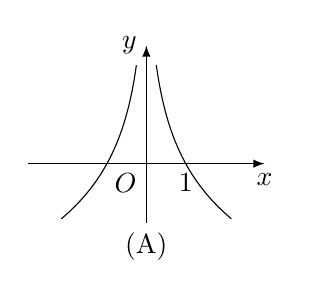
\begin{tikzpicture}[>=latex, scale = 0.5]
        \draw [->] (-3,0) -- (3,0) node [below] {$x$};
        \draw [->] (0,-1.5) -- (0,3) node [left] {$y$};
        \draw (0,0) node [below left] {$O$};
        \draw (1,0) node [below] {$1$};
        \draw [domain = -1.4:2.5] plot ({sqrt((1/3)^\x)},\x);
        \draw [domain = -1.4:2.5] plot ({-sqrt((1/3)^\x)},\x);
        \draw (0,-1.5) node [below] {(A)};
    \end{tikzpicture}
    \begin{tikzpicture}[>=latex, scale = 0.5]
        \draw [->] (-3,0) -- (3,0) node [below] {$x$};
        \draw [->] (0,-1.5) -- (0,3) node [left] {$y$};
        \draw (0,0) node [below left] {$O$};
        \draw (1,0) node [below] {$1$};
        \draw [domain = -0.9:2.5] plot ({-(1/3)^\x},\x);
        \draw (0,-1.5) node [below] {(B)};
    \end{tikzpicture}
    \begin{tikzpicture}[>=latex, scale = 0.5]
        \draw [->] (-3,0) -- (3,0) node [below] {$x$};
        \draw [->] (0,-1.5) -- (0,3) node [left] {$y$};
        \draw (0,0) node [below left] {$O$};
        \draw (1,0) node [below] {$1$};
        \draw [domain = -0.9:2.5] plot ({(1/3)^\x},{abs(\x)});
        \draw (0,-1.5) node [below] {(C)};
    \end{tikzpicture}
    \begin{tikzpicture}[>=latex, scale = 0.5]
        \draw [->] (-3,0) -- (3,0) node [below] {$x$};
        \draw [->] (0,-1.5) -- (0,3) node [left] {$y$};
        \draw (0,0) node [below left] {$O$};
        \draw (1,0) node [below] {$1$};
        \draw [domain = 0.1:2.5] plot (\x,{\x^(-1/3)});
        \draw (0,-1.5) node [below] {(D)};
    \end{tikzpicture}
\end{center}
\fourch{$y=\log_{\frac 13}x^2$}{$y=\log_{\frac 13}(-x)$}{$y=|\log_3x|$}{$y=|x^{-\frac 13}|$}


关联目标:

暂未关联目标



标签: 第二单元

答案: 暂无答案

解答或提示: 暂无解答与提示

使用记录:

暂无使用记录


出处: 代数精编第三章函数
\item { (005693)}在同一平面直角坐标系中画出函数$y=x+a$与$y=\log_ax$的图像, 可能是\bracket{20}.
\fourch{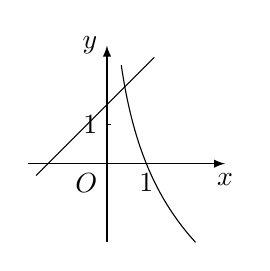
\begin{tikzpicture}[scale = 0.5, >=latex]
    \draw [->] (-2,0) -- (3,0) node [below] {$x$};
    \draw [->] (0,-2) -- (0,3) node [left] {$y$};
    \draw (0,0) node [below left] {$O$};
    \draw (1,0) node [below] {$1$};
    \draw (0.1,1) -- (0,1) node [left] {$1$};
    \draw [domain = -1.8:1.2] plot (\x,{\x+1.5});
    \draw [domain = -2.5:2] plot ({1.5^\x},{-\x}); 
\end{tikzpicture}}
{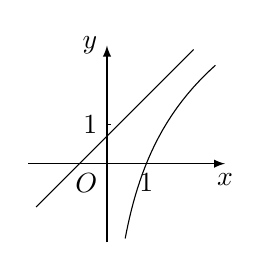
\begin{tikzpicture}[scale = 0.5, >=latex]
    \draw [->] (-2,0) -- (3,0) node [below] {$x$};
    \draw [->] (0,-2) -- (0,3) node [left] {$y$};
    \draw (0,0) node [below left] {$O$};
    \draw (1,0) node [below] {$1$};
    \draw (0.1,1) -- (0,1) node [left] {$1$};
    \draw [domain = -1.8:2.2] plot (\x,{\x+0.7}); 
    \draw [domain = -1.9:2.5] plot ({1.5^\x},{\x}); 
\end{tikzpicture}}
{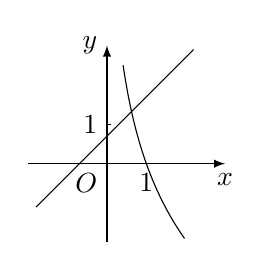
\begin{tikzpicture}[scale = 0.5, >=latex]
    \draw [->] (-2,0) -- (3,0) node [below] {$x$};
    \draw [->] (0,-2) -- (0,3) node [left] {$y$};
    \draw (0,0) node [below left] {$O$};
    \draw (1,0) node [below] {$1$};
    \draw (0.1,1) -- (0,1) node [left] {$1$};
    \draw [domain = -1.8:2.2] plot (\x,{\x+0.7}); 
    \draw [domain = -1.9:2.5] plot ({0.7^\x},{\x}); 
\end{tikzpicture}}
{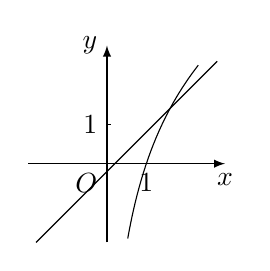
\begin{tikzpicture}[scale = 0.5, >=latex]
    \draw [->] (-2,0) -- (3,0) node [below] {$x$};
    \draw [->] (0,-2) -- (0,3) node [left] {$y$};
    \draw (0,0) node [below left] {$O$};
    \draw (1,0) node [below] {$1$};
    \draw (0.1,1) -- (0,1) node [left] {$1$};
    \draw [domain = -1.8:2.8] plot (\x,{\x-0.2}); 
    \draw [domain = -1.9:2.5] plot ({1.4^\x},{\x}); 
\end{tikzpicture}}


关联目标:

暂未关联目标



标签: 第二单元

答案: 暂无答案

解答或提示: 暂无解答与提示

使用记录:

暂无使用记录


出处: 代数精编第三章函数
\item { (005694)}函数$y=f(x)$的图像如图所示, 则$y=\log_{0.7}f(x)$的示意图是\bracket{20}.
\begin{center}
    \begin{tikzpicture}[>=latex]
        \draw [->] (-0.5,0) -- (3,0) node [below] {$x$};
        \draw [->] (0,-0.5) -- (0,3) node [left] {$y$};
        \draw (0,0) node [below left] {$O$};
        \draw (1,0.1) -- (1,0) node [below] {$1$} (2,0.1) -- (2,0) node [below] {$2$} (0.1,1) -- (0,1) node [left] {$1$};
        \draw [dashed] (2,0) -- (2,3);
        \draw [dashed] (1,0) -- (1,1) -- (0,1);
        \draw [domain = 0.3:1.7] plot (\x,{3*(\x-1)^2+1});
    \end{tikzpicture}
\end{center}
\fourch{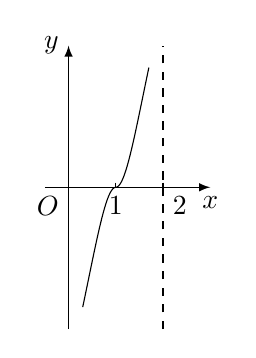
\begin{tikzpicture}[>=latex,scale = 0.6]
    \draw [->] (-0.5,0) -- (3,0) node [below] {$x$};
    \draw [->] (0,-3) -- (0,3) node [left] {$y$};
    \draw (0,0) node [below left] {$O$};
    \draw (1,0.1) -- (1,0) node [below] {$1$} (2,0.1) -- (2,0) node [below right] {$2$};
    \draw [dashed] (2,-3) -- (2,3);
    \draw [domain = 0.3:1] plot (\x,{ln(3*(\x-1)^2+1)/ln(0.7)});
    \draw [domain = 1:1.7] plot (\x,{-ln(3*(\x-1)^2+1)/ln(0.7)});
\end{tikzpicture}}{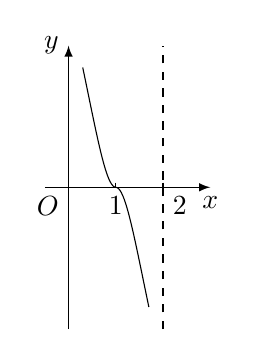
\begin{tikzpicture}[>=latex,scale = 0.6]
    \draw [->] (-0.5,0) -- (3,0) node [below] {$x$};
    \draw [->] (0,-3) -- (0,3) node [left] {$y$};
    \draw (0,0) node [below left] {$O$};
    \draw (1,0.1) -- (1,0) node [below] {$1$} (2,0.1) -- (2,0) node [below right] {$2$};
    \draw [dashed] (2,-3) -- (2,3);
    \draw [domain = 0.3:1] plot (\x,{-ln(3*(\x-1)^2+1)/ln(0.7)});
    \draw [domain = 1:1.7] plot (\x,{ln(3*(\x-1)^2+1)/ln(0.7)});
\end{tikzpicture}}{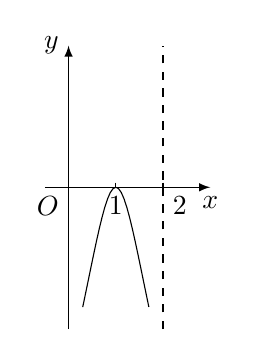
\begin{tikzpicture}[>=latex,scale = 0.6]
    \draw [->] (-0.5,0) -- (3,0) node [below] {$x$};
    \draw [->] (0,-3) -- (0,3) node [left] {$y$};
    \draw (0,0) node [below left] {$O$};
    \draw (1,0.1) -- (1,0) node [below] {$1$} (2,0.1) -- (2,0) node [below right] {$2$};
    \draw [dashed] (2,-3) -- (2,3);
    \draw [domain = 0.3:1.7] plot (\x,{ln(3*(\x-1)^2+1)/ln(0.7)});
\end{tikzpicture}}{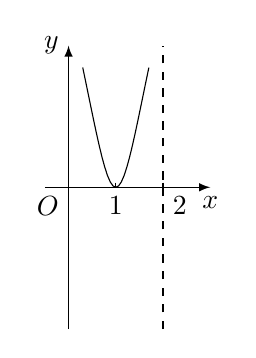
\begin{tikzpicture}[>=latex,scale = 0.6]
    \draw [->] (-0.5,0) -- (3,0) node [below] {$x$};
    \draw [->] (0,-3) -- (0,3) node [left] {$y$};
    \draw (0,0) node [below left] {$O$};
    \draw (1,0.1) -- (1,0) node [below] {$1$} (2,0.1) -- (2,0) node [below right] {$2$};
    \draw [dashed] (2,-3) -- (2,3);
    \draw [domain = 0.3:1.7] plot (\x,{-ln(3*(\x-1)^2+1)/ln(0.7)});
\end{tikzpicture}}


关联目标:

暂未关联目标



标签: 第二单元

答案: 暂无答案

解答或提示: 暂无解答与提示

使用记录:

暂无使用记录


出处: 代数精编第三章函数
\item { (005695)}由关系式$\log_xy=3$所确定的函数$y=f(x)$的图像是\bracket{20}.
\fourch{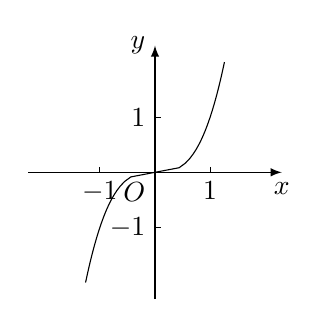
\begin{tikzpicture}[>=latex,scale = 0.7]
    \draw [->] (-2.3,0) -- (2.3,0) node [below] {$x$};
    \draw [->] (0,-2.3) -- (0,2.3) node [left] {$y$};
    \draw (0,0) node [below left] {$O$};
    \draw (1,0.1) -- (1,0) node [below] {$1$} (-1,0.1) -- (-1,0) node [below] {$-1$} (0.1,1) -- (0,1) node [left] {$1$} (0.1,-1) -- (0,-1) node [left] {$-1$};
    \draw [domain = 0:2] plot ({\x^(1/3)},\x);
    \draw [domain = 0:2] plot ({-\x^(1/3)},{-\x});
\end{tikzpicture}}{\begin{tikzpicture}[>=latex,scale = 0.7]
    \draw [->] (-2.3,0) -- (2.3,0) node [below] {$x$};
    \draw [->] (0,-2.3) -- (0,2.3) node [left] {$y$};
    \draw (0,0) node [below left] {$O$};
    \draw (1,0.1) -- (1,0) node [below] {$1$} (-1,0.1) -- (-1,0) node [below] {$-1$} (0.1,1) -- (0,1) node [left] {$1$} (0.1,-1) -- (0,-1) node [left] {$-1$};
    \draw [domain = 0:2] plot ({\x^(1/3)},\x);
    \filldraw [white] (0,0) circle (0.05) (1,1) circle (0.05);
    \draw (0,0) circle (0.05) (1,1) circle (0.05);
\end{tikzpicture}}{\begin{tikzpicture}[>=latex,scale = 0.7]
    \draw [->] (-2.3,0) -- (2.3,0) node [below] {$x$};
    \draw [->] (0,-2.3) -- (0,2.3) node [left] {$y$};
    \draw (0,0) node [below left] {$O$};
    \draw (1,0.1) -- (1,0) node [below] {$1$} (-1,0.1) -- (-1,0) node [below] {$-1$} (0.1,1) -- (0,1) node [left] {$1$} (0.1,-1) -- (0,-1) node [left] {$-1$};
    \draw [domain = 0:2] plot ({\x^(1/3)},\x);
\end{tikzpicture}}{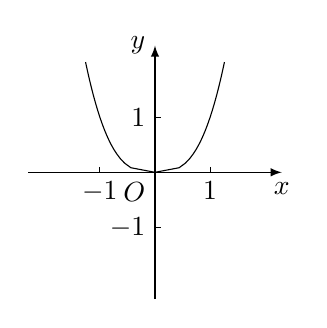
\begin{tikzpicture}[>=latex,scale = 0.7]
    \draw [->] (-2.3,0) -- (2.3,0) node [below] {$x$};
    \draw [->] (0,-2.3) -- (0,2.3) node [left] {$y$};
    \draw (0,0) node [below left] {$O$};
    \draw (1,0.1) -- (1,0) node [below] {$1$} (-1,0.1) -- (-1,0) node [below] {$-1$} (0.1,1) -- (0,1) node [left] {$1$} (0.1,-1) -- (0,-1) node [left] {$-1$};
    \draw [domain = 0:2] plot ({\x^(1/3)},\x);
    \draw [domain = 0:2] plot ({-\x^(1/3)},\x);
\end{tikzpicture}}


关联目标:

暂未关联目标



标签: 第二单元

答案: 暂无答案

解答或提示: 暂无解答与提示

使用记录:

暂无使用记录


出处: 代数精编第三章函数
\item { (005696)}若函数$f(x)=\dfrac{1-2^x}{1+2^x}$, 则$f^{-1}(\dfrac 35)$等于\bracket{20}.
\fourch{$3$}{$2$}{$1$}{$-2$}


关联目标:

暂未关联目标



标签: 第二单元

答案: 暂无答案

解答或提示: 暂无解答与提示

使用记录:

暂无使用记录


出处: 代数精编第三章函数
\item { (005697)}函数$y=\log_{\frac 13}(x^2-3x+4)$的定义域为\blank{50}.


关联目标:

暂未关联目标



标签: 第二单元

答案: 暂无答案

解答或提示: 暂无解答与提示

使用记录:

暂无使用记录


出处: 代数精编第三章函数
\item { (005698)}函数$y=\dfrac{\sqrt {x^2-4}}{\lg (x^2+2x-3)}$的定义域为\blank{50}.


关联目标:

暂未关联目标



标签: 第二单元

答案: 暂无答案

解答或提示: 暂无解答与提示

使用记录:

暂无使用记录


出处: 代数精编第三章函数
\item { (005699)}函数$y=\log_{(2x-1)}(32-4^x)$的定义域为\blank{50}.


关联目标:

暂未关联目标



标签: 第二单元

答案: 暂无答案

解答或提示: 暂无解答与提示

使用记录:

暂无使用记录


出处: 代数精编第三章函数
\item { (005700)}函数$y=\log_{\frac 13}(x^2-4x+7)$的值域为\blank{50}.


关联目标:

暂未关联目标



标签: 第二单元

答案: 暂无答案

解答或提示: 暂无解答与提示

使用记录:

暂无使用记录


出处: 代数精编第三章函数
\item { (005701)}函数$y=\log_{\frac 12}\dfrac 1{x^2-2x+5}$的值域为\blank{50}.


关联目标:

暂未关联目标



标签: 第二单元

答案: 暂无答案

解答或提示: 暂无解答与提示

使用记录:

暂无使用记录


出处: 代数精编第三章函数
\item { (005702)}函数$y=\log_{\frac 12}\sqrt {3-2x-x^2}$的值域为\blank{50}.


关联目标:

暂未关联目标



标签: 第二单元

答案: 暂无答案

解答或提示: 暂无解答与提示

使用记录:

暂无使用记录


出处: 代数精编第三章函数
\item { (005703)}函数$y=\log_{\frac 13}(x^2-5x+6)$为减函数的区间是\blank{50}.


关联目标:

暂未关联目标



标签: 第二单元

答案: 暂无答案

解答或提示: 暂无解答与提示

使用记录:

暂无使用记录


出处: 代数精编第三章函数
\item { (005704)}函数$y=\lg (12-4x-x^2)$为增函数的区间是\blank{50}.


关联目标:

暂未关联目标



标签: 第二单元

答案: 暂无答案

解答或提示: 暂无解答与提示

使用记录:

暂无使用记录


出处: 代数精编第三章函数
\item { (005705)}函数$y=-\log_{\frac 12}(-x)$为减函数的区间是\blank{50}.


关联目标:

暂未关联目标



标签: 第二单元

答案: 暂无答案

解答或提示: 暂无解答与提示

使用记录:

暂无使用记录


出处: 代数精编第三章函数
\item { (005706)}若函数$y=\log_a(1-x)$在$[0,1)$上是增函数, 则$a$的取值范围是\blank{50}.


关联目标:

暂未关联目标



标签: 第二单元

答案: 暂无答案

解答或提示: 暂无解答与提示

使用记录:

暂无使用记录


出处: 代数精编第三章函数
\item { (005707)}函数$y=\log_{\frac 12}^2x-\log_{\frac 12}x+1$为增函数的区间是\blank{50}.


关联目标:

暂未关联目标



标签: 第二单元

答案: 暂无答案

解答或提示: 暂无解答与提示

使用记录:

暂无使用记录


出处: 代数精编第三章函数
\item { (005709)}函数$y=1+\lg (x+2)$($x\ge 8$)的反函数是\blank{50}.


关联目标:

暂未关联目标



标签: 第二单元

答案: 暂无答案

解答或提示: 暂无解答与提示

使用记录:

暂无使用记录


出处: 代数精编第三章函数
\item { (005710)}若$f(x)=\dfrac{10^x+1}{10^x-1}$($x>1$), 则$f^{-1}(\dfrac{101}{99})=$\blank{50}.


关联目标:

暂未关联目标



标签: 第二单元

答案: 暂无答案

解答或提示: 暂无解答与提示

使用记录:

暂无使用记录


出处: 代数精编第三章函数
\item { (005711)}若$f(x)=\dfrac{\lg x-1}{\lg x+1}$($x>1$且$x\ne \dfrac 1{10}$), 则$f^{-1}(\dfrac 1{10})=$\blank{50}.


关联目标:

暂未关联目标



标签: 第二单元

答案: 暂无答案

解答或提示: 暂无解答与提示

使用记录:

暂无使用记录


出处: 代数精编第三章函数
\item { (005712)}若函数$f(x)=a^x-k$的图像过点$(1, 3)$, 其反函数$f^{-1}(x)$的图像过点$(2, 0)$, 则$f(x)$的表达式是\blank{50}.


关联目标:

暂未关联目标



标签: 第二单元

答案: 暂无答案

解答或提示: 暂无解答与提示

使用记录:

暂无使用记录


出处: 代数精编第三章函数
\item { (005713)}函数$y=\lg \dfrac{1-x}{1+x}$\bracket{20}.
\twoch{是奇函数, 且在$(-1, 1)$是增函数}{是奇函数, 且在$(-1, 1)$上是减函数}{是偶函数, 且在$(-1, 1)$是增函数}{是偶函数, 且在$(-1, 1)$上是减函数}


关联目标:

暂未关联目标



标签: 第二单元

答案: 暂无答案

解答或提示: 暂无解答与提示

使用记录:

暂无使用记录


出处: 代数精编第三章函数
\item { (005714)}函数$f(x)=\ln (\mathrm{e}^x+1)-\dfrac x2$\bracket{20}.
\twoch{是奇函数, 但不是偶函数}{是偶函数, 但不是奇函数}{既是奇函数, 又是偶函数}{没有奇偶性}


关联目标:

暂未关联目标



标签: 第二单元

答案: 暂无答案

解答或提示: 暂无解答与提示

使用记录:

暂无使用记录


出处: 代数精编第三章函数
\item { (005715)}求函数$f(x)=\lg (1+x)+\lg (1-x)$ $(-\dfrac 12<x<0)$的反函数.


关联目标:

暂未关联目标



标签: 第二单元

答案: 暂无答案

解答或提示: 暂无解答与提示

使用记录:

暂无使用记录


出处: 代数精编第三章函数
\item { (005716)}已知$f(x)=\dfrac{a^x-1}{a^x+1}$($a>1$).\\
(1) 求$f(x)$的值域;\\
(2) 求证: $f(x)$在$R$上是增函数;\\
(3) 求$f(x)$的反函数.


关联目标:

暂未关联目标



标签: 第二单元

答案: 暂无答案

解答或提示: 暂无解答与提示

使用记录:

暂无使用记录


出处: 代数精编第三章函数
\item { (005717)}已知$f(\log_ax)=\dfrac{a(x^2-1)}{x(a^2-1)}$($x>0$, $0<a<1$), 求证: 函数$f(x)$在$(-\infty ,+\infty)$上是增函数.


关联目标:

暂未关联目标



标签: 第二单元

答案: 暂无答案

解答或提示: 暂无解答与提示

使用记录:

暂无使用记录


出处: 代数精编第三章函数
\item { (005718)}若函数$f(x)=\log_a|x+1|$在$(-1, 0)$上有$f(x)>0$, 则$f(x)$\bracket{20}.
\twoch{在$(-\infty ,0)$上是增函数}{在$(-\infty ,0)$是减函数}{在$(-\infty ,-1)$上是增函数}{在$(-\infty ,-1)$是减函数}


关联目标:

暂未关联目标



标签: 第二单元

答案: 暂无答案

解答或提示: 暂无解答与提示

使用记录:

暂无使用记录


出处: 代数精编第三章函数
\item { (005719)}若$0<b<1$, $\log_ab<1$则\bracket{20}.
\fourch{$0<a<b$}{$0<b<a$}{$0<b<a<1$}{$0<a<b$或$a>1$}


关联目标:

暂未关联目标



标签: 第二单元

答案: 暂无答案

解答或提示: 暂无解答与提示

使用记录:

暂无使用记录


出处: 代数精编第三章函数
\item { (005720)}若函数$f(x)=|\log_ax|$, 其中$0<a<1$, 则下列各式中成立的是\bracket{20}.
\fourch{$f(\dfrac 13)>f(2)>f(\dfrac 14)$}{$f(\dfrac 14)>f(\dfrac 13)>f(2)$}{$f(2)>f(\dfrac 13)>f(\dfrac 14)$}{$f(\dfrac 14)>f(2)>f(\dfrac 13)$}


关联目标:

暂未关联目标



标签: 第二单元

答案: 暂无答案

解答或提示: 暂无解答与提示

使用记录:

暂无使用记录


出处: 代数精编第三章函数
\item { (005721)}若$1<x<2$, 则下列各式正确的是\bracket{20}.
\fourch{$2^x>\log_{\frac 12}x>\sqrt[3]x$}{$2^x>\sqrt[3]x>\log_{\frac 12}x$}{$\sqrt[3]x>2^x>\log_{\frac 12}x$}{$\log_{\frac 12}>x\sqrt[3]x>2^x$}


关联目标:

暂未关联目标



标签: 第二单元

答案: 暂无答案

解答或提示: 暂无解答与提示

使用记录:

暂无使用记录


出处: 代数精编第三章函数
\item { (005722)}若函数$f(x)=\log_ax$在$x\in [3,+\infty)$上恒有$|f(x)|>1$, 则实数$a$的取值范围是\bracket{20}.
\twoch{$0<a<\dfrac 13$或$1<a<3$}{$0<a<\dfrac 13$或$a>3$}{$\dfrac 13<a<3$且$a\ne 1$}{$\dfrac 13<a<1$或$a>3$}


关联目标:

暂未关联目标



标签: 第二单元

答案: 暂无答案

解答或提示: 暂无解答与提示

使用记录:

暂无使用记录


出处: 代数精编第三章函数
\item { (005723)}若$a>a^2>b>0$, 并记$p=\log_ab$, $q=\log_ba$, $r=\log_a\dfrac ab$, $s=\log_b\dfrac ba$, 则$p,q,r,s$的大小关系是\bracket{20}.
\fourch{$r<q<p<s$}{$r<p<q<s$}{$r<p<s<q$}{$r<q<s<p$}


关联目标:

暂未关联目标



标签: 第二单元

答案: 暂无答案

解答或提示: 暂无解答与提示

使用记录:

暂无使用记录


出处: 代数精编第三章函数
\item { (005724)}若$\log_a\dfrac 13>\log_b\dfrac 13>0$, 则$a,b$的关系是\bracket{20}.
\fourch{$1<b<a$}{$1<a<b$}{$0<a<b<1$}{$0<b<a<1$}


关联目标:

暂未关联目标



标签: 第二单元

答案: 暂无答案

解答或提示: 暂无解答与提示

使用记录:

暂无使用记录


出处: 代数精编第三章函数
\item { (005725)}将下列各数按从小到大排列: $a=|\log_{\frac 13}\dfrac 14|$, $b=|\log_{\frac 12}\dfrac 32|$, $c=|\log_25|$:\blank{50}.


关联目标:

暂未关联目标



标签: 第二单元

答案: 暂无答案

解答或提示: 暂无解答与提示

使用记录:

暂无使用记录


出处: 代数精编第三章函数
\item { (005726)}将下列各数按从小到大排列: $\log_{0.1}0.4$, $\log_{\frac 12}0.4$, $\log_30.4$, $\lg 0.4$:\blank{50}.


关联目标:

暂未关联目标



标签: 第二单元

答案: 暂无答案

解答或提示: 暂无解答与提示

使用记录:

暂无使用记录


出处: 代数精编第三章函数
\item { (005727)}将下列各数按从小到大排列: $\dfrac 32$, $\log_23$:\blank{50}.


关联目标:

暂未关联目标



标签: 第二单元

答案: 暂无答案

解答或提示: 暂无解答与提示

使用记录:

暂无使用记录


出处: 代数精编第三章函数
\item { (005728)}将下列各数按从小到大排列: $\dfrac 2{\lg 2}$, $\dfrac 3{\lg 3}$, $\dfrac 5{\lg 5}$:\blank{50}.


关联目标:

暂未关联目标



标签: 第二单元

答案: 暂无答案

解答或提示: 暂无解答与提示

使用记录:

暂无使用记录


出处: 代数精编第三章函数
\item { (005729)}将下列各数按从小到大排列: $\lg ^2x$, $\lg x^2$, $\lg (\lg x)$, 其中$1<x<10$:\blank{50}.


关联目标:

暂未关联目标



标签: 第二单元

答案: 暂无答案

解答或提示: 暂无解答与提示

使用记录:

暂无使用记录


出处: 代数精编第三章函数
\item { (005730)}若$\log_a\dfrac 45<1$($a>0$, $a\ne 1$), 则$a$的取值范围是\blank{50}.


关联目标:

暂未关联目标



标签: 第二单元

答案: 暂无答案

解答或提示: 暂无解答与提示

使用记录:

暂无使用记录


出处: 代数精编第三章函数
\item { (005731)}若$0<a<1$, $0<b<1$, 且$a^{\log_b(x-3)}<1$, 则$x$的取值范围是\blank{50}.


关联目标:

暂未关联目标



标签: 第二单元

答案: 暂无答案

解答或提示: 暂无解答与提示

使用记录:

暂无使用记录


出处: 代数精编第三章函数
\item { (005732)}求函数$y=(\log_{\frac 14}x)^2-\log_{\frac 14}x^2+5$($2\le x\le 4$)的值域.


关联目标:

暂未关联目标



标签: 第二单元

答案: 暂无答案

解答或提示: 暂无解答与提示

使用记录:

暂无使用记录


出处: 代数精编第三章函数
\item { (005733)}若$-3\le \log_{\frac 12}x\le -\dfrac 12$, 求$y=(\log_2\dfrac x2)(\log_2\dfrac x4)$的最大(小)值及其相应的$x$值,


关联目标:

暂未关联目标



标签: 第二单元

答案: 暂无答案

解答或提示: 暂无解答与提示

使用记录:

暂无使用记录


出处: 代数精编第三章函数
\item { (005734)}已知$a,b$是两个不相等的正数, 且$\log_m\dfrac xa\cdot \log_m\dfrac xb$的最小值是$-\dfrac 14$($m>0$且$m\ne 1$), 求$m$的值.


关联目标:

暂未关联目标



标签: 第二单元

答案: 暂无答案

解答或提示: 暂无解答与提示

使用记录:

暂无使用记录


出处: 代数精编第三章函数
\item { (005735)}已知实数$x,y$满足$(\log_4y)^2=\log_{\frac 12}x$, 求$u=\dfrac xy$的最大值及其相应的$x,y$的值.


关联目标:

暂未关联目标



标签: 第二单元

答案: 暂无答案

解答或提示: 暂无解答与提示

使用记录:

暂无使用记录


出处: 代数精编第三章函数
\item { (005736)}已知抛物线$y=x^2\log_2a+2x\log_a2+8$位于$x$轴的上方, 求实数$a$的取值范围.


关联目标:

暂未关联目标



标签: 第二单元

答案: 暂无答案

解答或提示: 暂无解答与提示

使用记录:

暂无使用记录


出处: 代数精编第三章函数
\item { (005737)}已知函数$f(x)=(\log_ab)x^2+2(\log_ba)x+8$的图像在$x$轴的上方, 求$a,b$的取值范围.


关联目标:

暂未关联目标



标签: 第二单元

答案: 暂无答案

解答或提示: 暂无解答与提示

使用记录:

暂无使用记录


出处: 代数精编第三章函数
\item { (005738)}若只有一个$x$的值满足方程$(1-\lg ^2a)x^2+(1-\lg a)x+2=0$, 求实数$a$的值.


关联目标:

暂未关联目标



标签: 第二单元

答案: 暂无答案

解答或提示: 暂无解答与提示

使用记录:

暂无使用记录


出处: 代数精编第三章函数
\item { (005739)}若关于$x$的方程$x^2+2(\log_3a+1)x-\log_9a=0$有两个相等实根, 求实数$a$的值.


关联目标:

暂未关联目标



标签: 第二单元

答案: 暂无答案

解答或提示: 暂无解答与提示

使用记录:

暂无使用记录


出处: 代数精编第三章函数
\item { (005740)}若二次函数$f(x)=(\lg a)x^2+2x+4\lg a$有最小值$-3$, 求实数$a$的值.


关联目标:

暂未关联目标



标签: 第二单元

答案: 暂无答案

解答或提示: 暂无解答与提示

使用记录:

暂无使用记录


出处: 代数精编第三章函数
\item { (005741)}已知$f(x)=\log_a|\log_ax|$($0<a<1$).\\
(1) 解不等式: $f(x)>0$;\\
(2) 判断$f(x)$在$(1,+\infty)$上的单调性, 并证明之.


关联目标:

暂未关联目标



标签: 第二单元

答案: 暂无答案

解答或提示: 暂无解答与提示

使用记录:

暂无使用记录


出处: 代数精编第三章函数
\item { (005742)}实数$a$为何值时, 函数$f(x)=2^x-2^{-x}\lg a$为奇函数?


关联目标:

暂未关联目标



标签: 第二单元

答案: 暂无答案

解答或提示: 暂无解答与提示

使用记录:

暂无使用记录


出处: 代数精编第三章函数
\item { (005743)}已知函数$f(x)=\sqrt {\log_ax-1}$($a>0$且$a\ne 1$).\\
(1) 求$f(x)$的定义域;\\
(2) 当$a>1$时, 求证: $f(x)$在$[a,+\infty)$上是增函数.


关联目标:

暂未关联目标



标签: 第二单元

答案: 暂无答案

解答或提示: 暂无解答与提示

使用记录:

暂无使用记录


出处: 代数精编第三章函数
\item { (005744)}已知函数$f(x)=1+\log_x3$, $g(x)=2\log_x2$($x>0$, 且$x\ne 1$), 比较$f(x)$与$g(x)$的大小.


关联目标:

暂未关联目标



标签: 第二单元

答案: 暂无答案

解答或提示: 暂无解答与提示

使用记录:

暂无使用记录


出处: 代数精编第三章函数
\item { (005745)}当$a>1$时, 比较$\log_ba$与$\log_{2b}a$的大小.


关联目标:

暂未关联目标



标签: 第二单元

答案: 暂无答案

解答或提示: 暂无解答与提示

使用记录:

暂无使用记录


出处: 代数精编第三章函数
\item { (005746)}已知$\log_ma>\log_na$($a>1$), 讨论$m$与$n$的大小关系.


关联目标:

暂未关联目标



标签: 第二单元

答案: 暂无答案

解答或提示: 暂无解答与提示

使用记录:

暂无使用记录


出处: 代数精编第三章函数
\item { (005747)}已知$\log_{1+a}(1-a)<1$, 求实数$a$的取值范围.


关联目标:

暂未关联目标



标签: 第二单元

答案: 暂无答案

解答或提示: 暂无解答与提示

使用记录:

暂无使用记录


出处: 代数精编第三章函数
\item { (005748)}已知$|\lg (1-a)|>|\lg (1+a)|$, 求实数$a$的取值范围.


关联目标:

暂未关联目标



标签: 第二单元

答案: 暂无答案

解答或提示: 暂无解答与提示

使用记录:

暂无使用记录


出处: 代数精编第三章函数
\item { (005749)}已知函数$f(x)=\log_{\frac 12}(x^2-2x)$.\\
(1) 求它的单调区间;\\
(2) 求$f(x)$为增函数时的反函数.


关联目标:

暂未关联目标



标签: 第二单元

答案: 暂无答案

解答或提示: 暂无解答与提示

使用记录:

暂无使用记录


出处: 代数精编第三章函数
\item { (005750)}已知函数$f(x)=\log_a\dfrac{x+b}{x-b}$($a>0$, $b>0$且$a\ne 1$).\\
(1) 求$f(x)$的定义域;\\
(2) 讨论$f(x)$的奇偶性;\\
(3) 讨论$f(x)$的单调性;\\
(4) 求$f(x)$的反函数$f^{-1}(x)$.


关联目标:

暂未关联目标



标签: 第二单元

答案: 暂无答案

解答或提示: 暂无解答与提示

使用记录:

暂无使用记录


出处: 代数精编第三章函数
\item { (005751)}已知函数$f(x)=\lg \dfrac{x+1}{x-1}+\lg (x-1)+\lg (a-x)$($a>1$).\\
(1) 是否存在一个实数$a$使得函数$y=f(x)$的图像关于某一条垂直于$x$轴的直线对称? 若存在, 求出这个实数$a$; 若不存在, 说明理由;\\
(2) 当$f(x)$的最大值为2时, 求实数$a$的值.


关联目标:

暂未关联目标



标签: 第二单元

答案: 暂无答案

解答或提示: 暂无解答与提示

使用记录:

暂无使用记录


出处: 代数精编第三章函数
\item { (005752)}解方程$9^{2x-1}=4^x$.


关联目标:

暂未关联目标



标签: 第二单元

答案: 暂无答案

解答或提示: 由题意. 可得$(\dfrac 92)^{2x}=9$, 所以$ 2x=\log_{\frac 92}9$, 故$x=\dfrac 12\log_{\frac 92}9$.

使用记录:

暂无使用记录


出处: 代数精编第三章函数
\item { (005753)}解方程$(\dfrac 1{27})^x=9^{1-x}$.


关联目标:

暂未关联目标



标签: 第二单元

答案: 暂无答案

解答或提示: 方程即为$3^{-3x}=3^{2-2x}$, 所以$ -3x=2-2x$, 故$x=-2$.

使用记录:

暂无使用记录


出处: 代数精编第三章函数
\item { (005754)}解方程$9^x-2\cdot 3^{x+1}-27=0$.


关联目标:

暂未关联目标



标签: 第二单元

答案: 暂无答案

解答或提示: 令$y=3^x>0$, 则原方程可化为$y^2-6y-27=0$.
由此得$y=9$(另一解$y=-3$舍去).从而由$3^x=9$, 解得$x=2$.

使用记录:

暂无使用记录


出处: 代数精编第三章函数
\item { (005755)}解方程$9^x+4^x=\dfrac 52\times 6^x$.


关联目标:

暂未关联目标



标签: 第二单元

答案: 暂无答案

解答或提示: 方程即为$2\times 3^{2x}-5\times 3^x\times 2^x+2\times 2^{2x}=0$, 即$2(\dfrac 32)^{2x}-5\times (\dfrac 32)^x+2=0$.
令$y=(\dfrac 32)^x$, 方程又化为$2y^2-5y+2=0$, 解得$y_1=2$, $y_2=\dfrac 12$,
于是便可得$x_1=\log_{\frac 23}2$, $x_2=\log_{\frac 23}2$.

使用记录:

暂无使用记录


出处: 代数精编第三章函数
\item { (005756)}解方程$\log_3(3^x-1)\cdot \log_3(3^{x-1}-\dfrac 13)=2$.


关联目标:

暂未关联目标



标签: 第二单元

答案: 暂无答案

解答或提示: 方程即为$\log_3(3^x-1)\cdot \log_3[\dfrac 13(3^x-1)]=2$.
令$t=\log_3(3^x-1)$, 则方程可化为$t(t-1)-2=0$, 解得$t_1=2$, $t_2=-1$.
于是由$\log_3(3^x-1)=2$, 得$3^x=10$, 所以$ x=\log_310$.
由$\log_3(3^x-1)=-1$, 得$3^x=\dfrac 43$, 所以$ x=\log_3\dfrac 43$.
故原方程的解为$x_1=\log_310$, $x_2=\log_3\dfrac 43$.

使用记录:

暂无使用记录


出处: 代数精编第三章函数
\item { (005757)}已知关于$x$的方程$\lg (kx)=2\lg (x+1)$有且只有一个实数解, 求实数$k$的取值范围.


关联目标:

暂未关联目标



标签: 第二单元

答案: 暂无答案

解答或提示: 显然, $x$需满足
$\begin{cases} kx>0, \\ x+1>0, \\ (x+1)^2=kx, \end{cases}$即$\begin{cases} x>-1, \\ x^2+(2-k)x+1=0. \end{cases}$.
(1) 若上述方程有两个相等实根, 则必有$\Delta =0$, 即$(2-k)^2-4=0$,
所以$ k=0$或$k=4$.
若$k=0$, 得实根$x=-1$应舍去; 若$k=4$, 得实根$x=1$符合题意.
(2) 若上述方程有两个不等实根$x_1,x_2$,
则必有$x_1>-1$, $x_2\le -1$.
考虑函数$f(x)=x^2+(2-k)x+1$.
\begin{center}
    \begin{tikzpicture}
        \draw [->] (-2,0) -- (2,0) node [below] {$x$};
        \draw [->] (0,-2) -- (0,2) node [left] {$y$};
        \draw (0,0) node [below right] {$O$};
        \draw [dashed] (-1,-2) -- (-1,0) node [below right] {$-1$} -- (-1,2);
        \draw [domain = -1.5:1.6] plot (\x,{(\x-0.1)^2-1.5});
    \end{tikzpicture}
\end{center}
如图, 只需$f(-1)\le 0$, 即$1+(2-k)(-1)+1\le 0$,
所以$ k\le 0$. 由(1)知, $k=0$不合题意.
综上所述, 实数$k$的取值范围是$k=4$或$k<0$.

使用记录:

暂无使用记录


出处: 代数精编第三章函数
\item { (005758)}若$2^{2x}+4=5\times 2^x$, 则$x^2+1$等于\bracket{20}.
\fourch{$1$}{$5$}{$5$或$1$}{$3$或$2$}


关联目标:

暂未关联目标



标签: 第二单元

答案: 暂无答案

解答或提示: 暂无解答与提示

使用记录:

暂无使用记录


出处: 代数精编第三章函数
\item { (005759)}方程$2^{|x+1|}=3$的解集是\bracket{20}.
\fourch{$\{\log_{\frac 12}\dfrac 23\}$}{$\{\log_2\dfrac 23\}$}{$\{\log_2\dfrac 32,\log_2\dfrac 16\}$}{$\{\log_2\dfrac 13,-\log_{\frac 12}6\}$}


关联目标:

暂未关联目标



标签: 第二单元

答案: 暂无答案

解答或提示: 暂无解答与提示

使用记录:

暂无使用记录


出处: 代数精编第三章函数
\item { (005760)}方程$2x^2+2^x-3=0$的实数根有\bracket{20}.
\fourch{$0$个}{$1$个}{$2$个}{无数个}


关联目标:

暂未关联目标



标签: 第二单元

答案: 暂无答案

解答或提示: 暂无解答与提示

使用记录:

暂无使用记录


出处: 代数精编第三章函数
\item { (005762)}方程$6\cdot 7^{|x|}-7^{-x}=1$的解集是\bracket{20}.
\fourch{$\{\log_7\dfrac 12\}$}{$\{\log_75\}$}{$\{\log_7\dfrac 12,\log_75\}$}{$\varnothing$}


关联目标:

暂未关联目标



标签: 第二单元

答案: 暂无答案

解答或提示: 暂无解答与提示

使用记录:

暂无使用记录


出处: 代数精编第三章函数
\item { (005763)}若对于任意实数$p$, 函数$y=(p-1)2^x-\dfrac p2$的图像恒过一定点, 则这个点的坐标是\bracket{20}.
\fourch{$(1,-\dfrac 12)$}{$(0, -1)$}{$(-1,-\dfrac 12)$}{$(-2,-\dfrac 14)$}


关联目标:

暂未关联目标



标签: 第二单元

答案: 暂无答案

解答或提示: 暂无解答与提示

使用记录:

暂无使用记录


出处: 代数精编第三章函数
\item { (005765)}方程$3^{x^2}=(3^x)^2$的解为\blank{50}.


关联目标:

暂未关联目标



标签: 第二单元

答案: 暂无答案

解答或提示: 暂无解答与提示

使用记录:

暂无使用记录


出处: 代数精编第三章函数
\item { (005766)}方程$3^x=2^x$的解为\blank{50}.


关联目标:

暂未关联目标



标签: 第二单元

答案: 暂无答案

解答或提示: 暂无解答与提示

使用记录:

暂无使用记录


出处: 代数精编第三章函数
\item { (005768)}方程$5^{x-1}\cdot 10^{3x}=8^x$的解为\blank{50}.


关联目标:

暂未关联目标



标签: 第二单元

答案: 暂无答案

解答或提示: 暂无解答与提示

使用记录:

暂无使用记录


出处: 代数精编第三章函数
\item { (005770)}方程$2\cdot 4^x-7\cdot 2^x+3=0$的解为\blank{50}.


关联目标:

暂未关联目标



标签: 第二单元

答案: 暂无答案

解答或提示: 暂无解答与提示

使用记录:

暂无使用记录


出处: 代数精编第三章函数
\item { (005771)}方程$9^x-3^{x+2}-10=0$的解为\blank{50}.


关联目标:

暂未关联目标



标签: 第二单元

答案: 暂无答案

解答或提示: 暂无解答与提示

使用记录:

暂无使用记录


出处: 代数精编第三章函数
\item { (005773)}已知$a>0$且$a\ne 1$, 则方程$a(a^x+1)=a^{-x}+1$的解为\blank{50}.


关联目标:

暂未关联目标



标签: 第二单元

答案: 暂无答案

解答或提示: 暂无解答与提示

使用记录:

暂无使用记录


出处: 代数精编第三章函数
\item { (005774)}解方程: $3\times 16^x+36^x=2\times 81^x$.


关联目标:

暂未关联目标



标签: 第二单元

答案: 暂无答案

解答或提示: 暂无解答与提示

使用记录:

暂无使用记录


出处: 代数精编第三章函数
\item { (005775)}解方程: $(\sqrt {5+2\sqrt 6})^x+(\sqrt {5-2\sqrt 6})^x=10$.


关联目标:

暂未关联目标



标签: 第二单元

答案: 暂无答案

解答或提示: 暂无解答与提示

使用记录:

暂无使用记录


出处: 代数精编第三章函数
\item { (005779)}解关于$x$的方程$\dfrac{a^x-a^{-x}}{a^x+a^{-x}}=b$(实数$a>0$, $a\ne 1$, $b\in \mathbf{R}$).


关联目标:

暂未关联目标



标签: 第二单元

答案: 暂无答案

解答或提示: 暂无解答与提示

使用记录:

暂无使用记录


出处: 代数精编第三章函数
\item { (005780)}若关于$x$的指数方程$9^x+(a+4)3^x+4=0$有实数解, 试求实数$a$的取值范围.


关联目标:

暂未关联目标



标签: 第二单元

答案: 暂无答案

解答或提示: 暂无解答与提示

使用记录:

暂无使用记录


出处: 代数精编第三章函数
\item { (005782)}方程$\lg (x-1)^2=2$的解集是\bracket{20}.
\fourch{$\{11\}$}{$\{-9\}$}{$\{11,-9\}$}{$\{-11,9\}$}


关联目标:

暂未关联目标



标签: 第二单元

答案: 暂无答案

解答或提示: 暂无解答与提示

使用记录:

暂无使用记录


出处: 代数精编第三章函数
\item { (005783)}关于$x$的方程$\log_ax^2=\log_a(\sqrt {a+1}-\sqrt a)-\log_a(\sqrt {a+1}+\sqrt a)$($a>0$且$a\ne 1$)的解为\bracket{20}.
\fourch{$\sqrt {a+1}+\sqrt a$}{$\sqrt {a+1}-\sqrt a$}{$\pm (\sqrt {a+1}+\sqrt a)$}{$\pm (\sqrt {a+1}-\sqrt a)$}


关联目标:

暂未关联目标



标签: 第二单元

答案: 暂无答案

解答或提示: 暂无解答与提示

使用记录:

暂无使用记录


出处: 代数精编第三章函数
\item { (005784)}若$f(x)=1+\lg x$, $g(x)=x^2$, 则使$2f[g(x)]=g[f(x)]$成立的$x$值等于\bracket{20}.
\fourch{$10^{1+\sqrt 2}$或$10^{1-\sqrt 2}$}{$1+\sqrt 2$或$1-\sqrt 2$}{$10^{1+\sqrt 3}$或$10^{1-\sqrt 3}$}{$1+\sqrt 3$或$1-\sqrt 3$}


关联目标:

暂未关联目标



标签: 第二单元

答案: 暂无答案

解答或提示: 暂无解答与提示

使用记录:

暂无使用记录


出处: 代数精编第三章函数
\item { (005785)}方程$\log_5(x-8)^2=2+\log_5(x-2)$的解是\bracket{20}.
\fourch{3或$\dfrac 12$}{$\dfrac 12$}{$3$或$38$}{$2$}


关联目标:

暂未关联目标



标签: 第二单元

答案: 暂无答案

解答或提示: 暂无解答与提示

使用记录:

暂无使用记录


出处: 代数精编第三章函数
\item { (005786)}方程$\sqrt {\lg x-4}=4-\lg x$的解集是\bracket{20}.
\fourch{$\{100\}$}{$\{1000\}$}{$\{10000\}$}{$\{\dfrac 1{10000}\}$}


关联目标:

暂未关联目标



标签: 第二单元

答案: 暂无答案

解答或提示: 暂无解答与提示

使用记录:

暂无使用记录


出处: 代数精编第三章函数
\item { (005787)}方程$\log_2(x-1)-\log_4(x+5)=0$的解为\blank{50}.


关联目标:

暂未关联目标



标签: 第二单元

答案: 暂无答案

解答或提示: 暂无解答与提示

使用记录:

暂无使用记录


出处: 代数精编第三章函数
\item { (005788)}方程$\log_4(2-x)=\log_2(x-1)-1$的解为\blank{50}.


关联目标:

暂未关联目标



标签: 第二单元

答案: 暂无答案

解答或提示: 暂无解答与提示

使用记录:

暂无使用记录


出处: 代数精编第三章函数
\item { (005789)}方程$\log_x(x^2-x)=\log_x2$的解为\blank{50}.


关联目标:

暂未关联目标



标签: 第二单元

答案: 暂无答案

解答或提示: 暂无解答与提示

使用记录:

暂无使用记录


出处: 代数精编第三章函数
\item { (005790)}方程$\log_{(16-3x)}(x-2)=\log_82\sqrt 2$的解为\blank{50}.


关联目标:

暂未关联目标



标签: 第二单元

答案: 暂无答案

解答或提示: 暂无解答与提示

使用记录:

暂无使用记录


出处: 代数精编第三章函数
\item { (005791)}方程$\lg|2x-3|-\lg|3x-2|=0$的解为\blank{50}.


关联目标:

暂未关联目标



标签: 第二单元

答案: 暂无答案

解答或提示: 暂无解答与提示

使用记录:

暂无使用记录


出处: 代数精编第三章函数
\item { (005792)}方程$\lg ^2x+\lg x^3+2=0$的解为\blank{50}.


关联目标:

暂未关联目标



标签: 第二单元

答案: 暂无答案

解答或提示: 暂无解答与提示

使用记录:

暂无使用记录


出处: 代数精编第三章函数
\item { (005793)}方程$\lg ^2x+\lg x^2-3=0$的解为\blank{50}.


关联目标:

暂未关联目标



标签: 第二单元

答案: 暂无答案

解答或提示: 暂无解答与提示

使用记录:

暂无使用记录


出处: 代数精编第三章函数
\item { (005794)}方程$(\log_4x)^2-\dfrac 12|\log_2x|-2=0$的解为\blank{50}.


关联目标:

暂未关联目标



标签: 第二单元

答案: 暂无答案

解答或提示: 暂无解答与提示

使用记录:

暂无使用记录


出处: 代数精编第三章函数
\item { (005795)}已知方程$\ln ^2x-\ln x^2-2=0$的两个根为$\alpha ,\beta$, 求$\log_{\alpha }\beta +\log_{\beta }\alpha$的值.


关联目标:

暂未关联目标



标签: 第二单元

答案: 暂无答案

解答或提示: 暂无解答与提示

使用记录:

暂无使用记录


出处: 代数精编第三章函数
\item { (005796)}已知集合$A=\{x|x^2-ax+a^2-19=0\}$, $B=\{x|\log_2(x^2-5x+8)=1\}$, $C=\{x|x^2+2x-8=0\}$满足$A\cap B\ne \varnothing$, $A\cap C\ne \varnothing$, 求实数$a$的值.


关联目标:

暂未关联目标



标签: 第二单元

答案: 暂无答案

解答或提示: 暂无解答与提示

使用记录:

暂无使用记录


出处: 代数精编第三章函数
\item { (005797)}已知$f(x)=\log_a(a^x-1)$($a>0$, $a\ne 1$), 解方程$f(2x)=f^{-1}(x)$.


关联目标:

暂未关联目标



标签: 第二单元

答案: 暂无答案

解答或提示: 暂无解答与提示

使用记录:

暂无使用记录


出处: 代数精编第三章函数
\item { (005798)}解方程$\log_{\frac 12}(9^{x-1}-5)=\log_{\frac 12}(3^{x-1}-2)-2$.


关联目标:

暂未关联目标



标签: 第二单元

答案: 暂无答案

解答或提示: 暂无解答与提示

使用记录:

暂无使用记录


出处: 代数精编第三章函数
\item { (005799)}解方程$\log_{0.5x}2-\log_{0.5x^3}x^2=\log_{0.5x^3}4$.


关联目标:

暂未关联目标



标签: 第二单元

答案: 暂无答案

解答或提示: 暂无解答与提示

使用记录:

暂无使用记录


出处: 代数精编第三章函数
\item { (005800)}解方程$(\sqrt x)^{\log_5x-1}=5$.


关联目标:

暂未关联目标



标签: 第二单元

答案: 暂无答案

解答或提示: 暂无解答与提示

使用记录:

暂无使用记录


出处: 代数精编第三章函数
\item { (005801)}解方程$10^{\lg ^2x}+x^{\lg x}=20$.


关联目标:

暂未关联目标



标签: 第二单元

答案: 暂无答案

解答或提示: 暂无解答与提示

使用记录:

暂无使用记录


出处: 代数精编第三章函数
\item { (005802)}解方程$|\log_2x|=|\log_2(2x^2)|-2$.


关联目标:

暂未关联目标



标签: 第二单元

答案: 暂无答案

解答或提示: 暂无解答与提示

使用记录:

暂无使用记录


出处: 代数精编第三章函数
\item { (005803)}解方程组$\begin{cases} \log_yx-3\log_xy=2, \\ (2^x)^y=(\dfrac 12)^{-16}. \end{cases}$.


关联目标:

暂未关联目标



标签: 第二单元

答案: 暂无答案

解答或提示: 暂无解答与提示

使用记录:

暂无使用记录


出处: 代数精编第三章函数
\item { (005804)}解关于$x$的方程: $\lg (x+a)+1=\lg (ax-1)$.


关联目标:

暂未关联目标



标签: 第二单元

答案: 暂无答案

解答或提示: 暂无解答与提示

使用记录:

暂无使用记录


出处: 代数精编第三章函数
\item { (005805)}解关于$x$的方程: $\lg (ax-1)-\lg (x-3)=1$.


关联目标:

暂未关联目标



标签: 第二单元

答案: 暂无答案

解答或提示: 暂无解答与提示

使用记录:

暂无使用记录


出处: 代数精编第三章函数
\item { (005806)}解关于$x$的方程: $2\lg x-\lg (x-1)=\lg a$.


关联目标:

暂未关联目标



标签: 第二单元

答案: 暂无答案

解答或提示: 暂无解答与提示

使用记录:

暂无使用记录


出处: 代数精编第三章函数
\item { (005807)}已知函数$f(x)=a^{x-\dfrac 12}$满足$f(\lg a)=\sqrt {10}$, 求实数$a$的值.


关联目标:

暂未关联目标



标签: 第二单元

答案: 暂无答案

解答或提示: 暂无解答与提示

使用记录:

暂无使用记录


出处: 代数精编第三章函数
\item { (005808)}已知函数$f(x)=x^2-x+k$满足$\log_2f(a)=2$, $f(\log_2a)=k$($a>0$且$a\ne 1$), 求$f(\log_2x)$在什么区间上是减函数, 并求出$a$与$k$的值.


关联目标:

暂未关联目标



标签: 第二单元

答案: 暂无答案

解答或提示: 暂无解答与提示

使用记录:

暂无使用记录


出处: 代数精编第三章函数
\item { (005809)}若关于$x$的方程$\lg 2x\cdot \lg 3x=-a^2$有两个相异实根, 求实数$a$的取值范围, 并求此方程两根之积.


关联目标:

暂未关联目标



标签: 第二单元

答案: 暂无答案

解答或提示: 暂无解答与提示

使用记录:

暂无使用记录


出处: 代数精编第三章函数
\item { (005810)}若关于$x$的方程$(\lg ax)(\lg ax^2)=4$所有的解都大于$1$, 求实数$a$的取值范围.


关联目标:

暂未关联目标



标签: 第二单元

答案: 暂无答案

解答或提示: 暂无解答与提示

使用记录:

暂无使用记录


出处: 代数精编第三章函数
\item { (005811)}若关于$x$的方程$\lg (ax)\cdot \lg (ax^2)=4$有两个小于$1$的正根$\alpha ,\beta$, 且满足$|\lg \alpha -\lg \beta|\le 2\sqrt 3$, 求实数$a$的取值范围.


关联目标:

暂未关联目标



标签: 第二单元

答案: 暂无答案

解答或提示: 暂无解答与提示

使用记录:

暂无使用记录


出处: 代数精编第三章函数
\item { (005812)}已知函数$f(x)=x^2\lg a+2x+4\lg a$的最大值是$3$, 求实数$a$的值.


关联目标:

暂未关联目标



标签: 第二单元

答案: 暂无答案

解答或提示: 暂无解答与提示

使用记录:

暂无使用记录


出处: 代数精编第三章函数
\item { (005813)}若关于$x$的方程$\log_2x+1=2\log_2(x-a)$恰有一个实数解, 求实数$a$的取值范围.


关联目标:

暂未关联目标



标签: 第二单元

答案: 暂无答案

解答或提示: 暂无解答与提示

使用记录:

暂无使用记录


出处: 代数精编第三章函数
\item { (005814)}已知函数$f(x)=\log_a(a-ka^x)$($a>0$, $a\ne 1$, $k\in \mathbf{R}$).
(1) 当$0<a<1$, 且$1\le x$时, $f(x)$都有意义, 求实数$k$的取值范围;\\
(2) 当$a>1$时, $f(x)$的反函数就是它自身, 求$k$的值;\\
(3) 在(2)的条件下, 求$f^{-1}(x^2-2)=f(x)$的解.


关联目标:

暂未关联目标



标签: 第二单元

答案: 暂无答案

解答或提示: 暂无解答与提示

使用记录:

暂无使用记录


出处: 代数精编第三章函数
\item { (005850)}已知函数$f(x)=\log_3(x^2-4mx+4m^2+m+\dfrac 1{m-1})$, 集合$M=\{m|m>1,m\in \mathbf{R}\}$.\\
(1) 求证: 当$m\in M$时, $f(x)$的定义域为$x\in \mathbf{R}$; 反之, 若$f(x)$对一切实数$x$都有意义, 则$m\in M$;\\
(2) 当$m\in M$时, 求$f(x)$的最小值;\\
(3) 求证: 对每一个$m\in M$, $f(x)$的最小值都不小于1.


关联目标:

暂未关联目标



标签: 第二单元

答案: 暂无答案

解答或提示: 暂无解答与提示

使用记录:

暂无使用记录


出处: 代数精编第三章函数
\item { (005851)}已知函数$f(x)=\dfrac{4^x}{4^x+2}$, 求$f(\dfrac 1{101})+f(\dfrac 2{101})+\cdots +f(\dfrac{100}{101})$的值.


关联目标:

暂未关联目标



标签: 第二单元

答案: 暂无答案

解答或提示: 暂无解答与提示

使用记录:

暂无使用记录


出处: 代数精编第三章函数
\item { (005852)}已知函数$f(x)=1+\log_x5$, $g(x)=\log_{x^2}9+\log_{x^2}8$, 比较$f(x)$与$g(x)$的大小.


关联目标:

暂未关联目标



标签: 第二单元

答案: 暂无答案

解答或提示: 暂无解答与提示

使用记录:

暂无使用记录


出处: 代数精编第三章函数
\item { (005853)}求方程$x^2-4|x|-\log_2x-5=0$的实数解的个数.


关联目标:

暂未关联目标



标签: 第二单元

答案: 暂无答案

解答或提示: 暂无解答与提示

使用记录:

暂无使用记录


出处: 代数精编第三章函数
\item { (005855)}已知$f(x)$在$(-\infty ,+\infty)$上有单调性, 且满足$f(1)=2$和$f(x+y)=f(x)+f(y)$.\\
(1) 求证: $f(x)$为奇函数;\\
(2) 若$f(x)$满足$f(k\log_2t)+f(\log_2t-\log_2^2t-2)<0$, 求实数$k$的取值范围.


关联目标:

暂未关联目标



标签: 第二单元

答案: 暂无答案

解答或提示: 暂无解答与提示

使用记录:

暂无使用记录


出处: 代数精编第三章函数
\item { (005858)}解方程$|\log_2x|=|\log_22x^2|-2$.


关联目标:

暂未关联目标



标签: 第二单元

答案: 暂无答案

解答或提示: 暂无解答与提示

使用记录:

暂无使用记录


出处: 代数精编第三章函数
\item { (005859)}分别求实数$a$的取值范围, 使关于$x$的方程$\log_{(x+a)}2x=2$有唯一解、两解、无解.


关联目标:

暂未关联目标



标签: 第二单元

答案: 暂无答案

解答或提示: 暂无解答与提示

使用记录:

暂无使用记录


出处: 代数精编第三章函数
\item { (005860)}分别求实数$a$的范围, 使关于$x$的方程$1+\dfrac{\log_2(2\lg a-x)}{\log_2x}=2\log_x2$有两解、一解.


关联目标:

暂未关联目标



标签: 第二单元

答案: 暂无答案

解答或提示: 暂无解答与提示

使用记录:

暂无使用记录


出处: 代数精编第三章函数
\item { (007943)}已知幂函数$f(x)$的图像经过$(2,\dfrac{\sqrt 2}2)$, 试求出这个函数的解析式.


关联目标:

暂未关联目标



标签: 第二单元

答案: 暂无答案

解答或提示: 暂无解答与提示

使用记录:

暂无使用记录


出处: 二期课改练习册高一第一学期
\item { (007944)}幂函数$y=x^s$与$y=x^t$的图像在第一象限都通过定点\blank{50}, 若它们在第一象限的部分关于直线$y=x$对称, 则$s$、$t$应满足的条件是\blank{50}.


关联目标:

暂未关联目标



标签: 第二单元

答案: 暂无答案

解答或提示: 暂无解答与提示

使用记录:

暂无使用记录


出处: 二期课改练习册高一第一学期
\item { (007945)}研究幂函数$f(x)=x^{\frac 25}$的定义域、奇偶性、单调性、值域.


关联目标:

暂未关联目标



标签: 第二单元

答案: 暂无答案

解答或提示: 暂无解答与提示

使用记录:

暂无使用记录


出处: 二期课改练习册高一第一学期
\item { (007949)}已知幂函数$f(x)$的定义域是$(+\infty ,0)\cup (0,+\infty)$, 且它的图像关于$y$轴对称, 写出一个满足要求的幂函数$f(x)$.


关联目标:

暂未关联目标



标签: 第二单元

答案: 暂无答案

解答或提示: 暂无解答与提示

使用记录:

暂无使用记录


出处: 二期课改练习册高一第一学期
\item { (007953)}设$a^{2x}=2$, 且$a>0$, $a\ne 1$, 求$\dfrac{a^{3x}+a^{-3x}}{a^x+a^{-x}}$的值.


关联目标:

暂未关联目标



标签: 第二单元

答案: 暂无答案

解答或提示: 暂无解答与提示

使用记录:

暂无使用记录


出处: 二期课改练习册高一第一学期
\item { (007954)}已知$f(x)=a\cdot b^x$, $f(4)=648$, $f(5)=1944$.\\
(1) 估算$f(4.5)$;\\
(2) 计算$f(4.5)$, 利用计算的结果评判你的估算.


关联目标:

暂未关联目标



标签: 第二单元

答案: 暂无答案

解答或提示: 暂无解答与提示

使用记录:

暂无使用记录


出处: 二期课改练习册高一第一学期
\item { (007955)}已知$f(x)=3^x$, $u,v\in \mathbf{R}$.\\
(1) 求证: 对任意的$u$、$v$, 都有$f(u)\cdot f(v)=f(u+v)$成立.\\
(2) 写出一个关于$f(u)\div f(v)$类似上式的等式, 并证明你的结论.


关联目标:

暂未关联目标



标签: 第二单元

答案: 暂无答案

解答或提示: 暂无解答与提示

使用记录:

暂无使用记录


出处: 二期课改练习册高一第一学期
\item { (007956)}求证: $f(x)=\dfrac{a^x-a^{-x}}2$($a>0$, $a\ne 1$)是奇函数.


关联目标:

暂未关联目标



标签: 第二单元

答案: 暂无答案

解答或提示: 暂无解答与提示

使用记录:

暂无使用记录


出处: 二期课改练习册高一第一学期
\item { (007957)}求证: $f(x)=\dfrac{(a^x-1)\cdot x}{a^x+1}$($a>0$, $a\ne 1$)是偶函数.


关联目标:

暂未关联目标



标签: 第二单元

答案: 暂无答案

解答或提示: 暂无解答与提示

使用记录:

暂无使用记录


出处: 二期课改练习册高一第一学期
\item { (007958)}若指数函数$y=a^x$是减函数, 则下列不等式中, 能够成立的是\bracket{20}.
\fourch{$a>1$}{$a<1$}{$a(a-1)<0$}{$a(a-1)>0$}


关联目标:

暂未关联目标



标签: 第二单元

答案: 暂无答案

解答或提示: 暂无解答与提示

使用记录:

暂无使用记录


出处: 二期课改练习册高一第一学期
\item { (007959)}若函数$y=2^x-m$的图像不经过第二象限, 则$m$的取值范围是\bracket{20}.
\fourch{$m\ge 1$}{$m<1$}{$m>-1$}{$m\le -1$}


关联目标:

暂未关联目标



标签: 第二单元

答案: 暂无答案

解答或提示: 暂无解答与提示

使用记录:

暂无使用记录


出处: 二期课改练习册高一第一学期
\item { (007961)}已知集合$M=\{y|y=2^x,\ x\in \mathbf{R}\}$, 集合$N=\{y|y=x^2,\ x\in \mathbf{R}\}$, 求$M\cap N$.


关联目标:

暂未关联目标



标签: 第二单元

答案: 暂无答案

解答或提示: 暂无解答与提示

使用记录:

暂无使用记录


出处: 二期课改练习册高一第一学期
\item { (007964)}判断并证明函数$y=\dfrac{10^x-10^{-x}}{10^x+10^{-x}}$的奇偶性.


关联目标:

暂未关联目标



标签: 第二单元

答案: 暂无答案

解答或提示: 暂无解答与提示

使用记录:

暂无使用记录


出处: 二期课改练习册高一第一学期
\item { (007965)}判断并证明函数$y=x(\dfrac 1{2^x-1}+\dfrac 12)$的奇偶性.


关联目标:

暂未关联目标



标签: 第二单元

答案: 暂无答案

解答或提示: 暂无解答与提示

使用记录:

暂无使用记录


出处: 二期课改练习册高一第一学期
\item { (007966)}函数$y=4^x-2^{x+1}+1(x<0)$的值域是\bracket{20}.
\fourch{$[0,+\infty)$}{$(1,+\infty)$}{$(0,1)$}{$(0,1]$}


关联目标:

暂未关联目标



标签: 第二单元

答案: 暂无答案

解答或提示: 暂无解答与提示

使用记录:

暂无使用记录


出处: 二期课改练习册高一第一学期
\item { (007971)}幂函数$y=f(x)$, 当$x=2$时, $y=16$.\\
(1)求函数$f(x)$的解析式;\\
(2)比较$f(2)$和$f(-3)$的大小.


关联目标:

暂未关联目标



标签: 第二单元

答案: 暂无答案

解答或提示: 暂无解答与提示

使用记录:

暂无使用记录


出处: 二期课改练习册高一第一学期
\item { (007972)}若关于$x$的方程$5^x=\dfrac{a+3}{5-a}$有负数根, 则$a$的取值范围是\blank{50}.


关联目标:

暂未关联目标



标签: 第二单元

答案: 暂无答案

解答或提示: 暂无解答与提示

使用记录:

暂无使用记录


出处: 二期课改练习册高一第一学期
\item { (007973)}方程$(\dfrac 12)^x=x^{\frac 12}$的实数根个数为\blank{50}.


关联目标:

暂未关联目标



标签: 第二单元

答案: 暂无答案

解答或提示: 暂无解答与提示

使用记录:

暂无使用记录


出处: 二期课改练习册高一第一学期
\item { (007976)}当$x$充分大时, 试比较下列各函数: $y_1=10x,y_2=8x^2,y_3=4x^4,y_4=2\times 3^x,y_5=5^x$值的大小.你能从中归纳出一些规律性的结论吗?


关联目标:

暂未关联目标



标签: 第二单元

答案: 暂无答案

解答或提示: 暂无解答与提示

使用记录:

暂无使用记录


出处: 二期课改练习册高一第一学期
\item { (007977)}比较$a^2$和$a^a$两个值的大小(其中$a>0$, 且$a\ne 1$).


关联目标:

暂未关联目标



标签: 第二单元

答案: 暂无答案

解答或提示: 暂无解答与提示

使用记录:

暂无使用记录


出处: 二期课改练习册高一第一学期
\item { (007978)}比较$2^a$和$a^a$两个值的大小(其中$a>0$, 且$a\ne 1$).


关联目标:

暂未关联目标



标签: 第二单元

答案: 暂无答案

解答或提示: 暂无解答与提示

使用记录:

暂无使用记录


出处: 二期课改练习册高一第一学期
\item { (007983)}已知函数$f(x)=\begin{cases} -2^x-1, & x\le 0, \\x^{\frac 12}, & x>0. \end{cases}$若$f(x_0)=1$, 则$x_0$的值为\blank{50}.


关联目标:

暂未关联目标



标签: 第二单元

答案: 暂无答案

解答或提示: 暂无解答与提示

使用记录:

暂无使用记录


出处: 二期课改练习册高一第一学期
\item { (007987)}点$(\sqrt 2,2)$在幂函数$y=f(x)$的图像上, 点$(-2,\dfrac 14)$在幂函数$y=g(x)$的图像上.当$x$为何值时, $f(x)=g(x)$?


关联目标:

暂未关联目标



标签: 第二单元

答案: 暂无答案

解答或提示: 暂无解答与提示

使用记录:

暂无使用记录


出处: 二期课改练习册高一第一学期
\item { (007989)}已知函数$f(x)=a^x(a>0,a\ne 1)$在区间$[1,2]$上的最大值比最小值大$\dfrac 14$, 求实数$a$的值.


关联目标:

暂未关联目标



标签: 第二单元

答案: 暂无答案

解答或提示: 暂无解答与提示

使用记录:

暂无使用记录


出处: 二期课改练习册高一第一学期
\item { (007994)}若$2x+y=1$, 求$4^x+2^y$的最小值.


关联目标:

暂未关联目标



标签: 第二单元

答案: 暂无答案

解答或提示: 暂无解答与提示

使用记录:

暂无使用记录


出处: 二期课改练习册高一第一学期
\item { (008000)}把下列指数式写成对数式:\\
(1) $10^{-2}=0.01$:\blank{50};\\
(2) $(\dfrac 12)^0=1$:\blank{50};\\
(3) $5^x=6$:\blank{50}.


关联目标:

暂未关联目标



标签: 第二单元

答案: 暂无答案

解答或提示: 暂无解答与提示

使用记录:

暂无使用记录


出处: 二期课改练习册高一第二学期
\item { (008001)}把下列对数式写成指数式:\\
(1) $x=\log _{16}32$:\blank{50};\\
(2) $\log _{\pi }x=4$:\blank{50};\\
(3) $\log _x9=2$:\blank{50}.


关联目标:

暂未关联目标



标签: 第二单元

答案: 暂无答案

解答或提示: 暂无解答与提示

使用记录:

暂无使用记录


出处: 二期课改练习册高一第二学期
\item { (008002)}求下列各式中的$x$:\\
(1) $\log _{\frac 12}x=3$, $x=$\blank{50};\\
(2) $\log _3\dfrac 1{27}=x$, $x=$\blank{50};\\
(3) $\log _{100}1000=x$, $x=$\blank{50};\\
(4) $\log _x16=4$, $x=$\blank{50}.


关联目标:

暂未关联目标



标签: 第二单元

答案: 暂无答案

解答或提示: 暂无解答与提示

使用记录:

暂无使用记录


出处: 二期课改练习册高一第二学期
\item { (008003)}计算: $\log _55\sqrt 5+\ln e$.


关联目标:

暂未关联目标



标签: 第二单元

答案: 暂无答案

解答或提示: 暂无解答与提示

使用记录:

暂无使用记录


出处: 二期课改练习册高一第二学期
\item { (008004)}计算: $\lg \sqrt {10}-\lg 0.01$.


关联目标:

暂未关联目标



标签: 第二单元

答案: 暂无答案

解答或提示: 暂无解答与提示

使用记录:

暂无使用记录


出处: 二期课改练习册高一第二学期
\item { (008005)}计算: $\log _{12}6+\log _{12}2$.


关联目标:

暂未关联目标



标签: 第二单元

答案: 暂无答案

解答或提示: 暂无解答与提示

使用记录:

暂无使用记录


出处: 二期课改练习册高一第二学期
\item { (008006)}计算: $\log _348-4\log _32$.


关联目标:

暂未关联目标



标签: 第二单元

答案: 暂无答案

解答或提示: 暂无解答与提示

使用记录:

暂无使用记录


出处: 二期课改练习册高一第二学期
\item { (008007)}用$\log _aM$、$\log _aN$表示$\log _aMN^2$.


关联目标:

暂未关联目标



标签: 第二单元

答案: 暂无答案

解答或提示: 暂无解答与提示

使用记录:

暂无使用记录


出处: 二期课改练习册高一第二学期
\item { (008008)}用$\log _aM$、$\log _aN$表示$\log _a\dfrac{\sqrt M}N$.


关联目标:

暂未关联目标



标签: 第二单元

答案: 暂无答案

解答或提示: 暂无解答与提示

使用记录:

暂无使用记录


出处: 二期课改练习册高一第二学期
\item { (008009)}计算: $3^{\log _31}+\log _248-\log _23$.


关联目标:

暂未关联目标



标签: 第二单元

答案: 暂无答案

解答或提示: 暂无解答与提示

使用记录:

暂无使用记录


出处: 二期课改练习册高一第二学期
\item { (008010)}计算: $2\log _7\dfrac{35}9+4\log _73+2\log _7\dfrac 1{10}+\log _74$.


关联目标:

暂未关联目标



标签: 第二单元

答案: 暂无答案

解答或提示: 暂无解答与提示

使用记录:

暂无使用记录


出处: 二期课改练习册高一第二学期
\item { (008011)}计算: $\log _32\times \log _53\times \log _85$.


关联目标:

暂未关联目标



标签: 第二单元

答案: 暂无答案

解答或提示: 暂无解答与提示

使用记录:

暂无使用记录


出处: 二期课改练习册高一第二学期
\item { (008012)}计算: $(\log _43+\log _83)\times \log _32$.


关联目标:

暂未关联目标



标签: 第二单元

答案: 暂无答案

解答或提示: 暂无解答与提示

使用记录:

暂无使用记录


出处: 二期课改练习册高一第二学期
\item { (008013)}计算: $\log _2\dfrac 1{49}\times \log _3\dfrac 1{16}\times \log _7\dfrac 1{27}$.


关联目标:

暂未关联目标



标签: 第二单元

答案: 暂无答案

解答或提示: 暂无解答与提示

使用记录:

暂无使用记录


出处: 二期课改练习册高一第二学期
\item { (008014)}计算: $\log _ab\cdot \log _bc\cdot \log _ca$.


关联目标:

暂未关联目标



标签: 第二单元

答案: 暂无答案

解答或提示: 暂无解答与提示

使用记录:

暂无使用记录


出处: 二期课改练习册高一第二学期
\item { (008015)}计算: $(\log _43+\log _83)(\log _32+\log _94)$.


关联目标:

暂未关联目标



标签: 第二单元

答案: 暂无答案

解答或提示: 暂无解答与提示

使用记录:

暂无使用记录


出处: 二期课改练习册高一第二学期
\item { (008016)}已知$\log _32=m$, 试用$m$表示$\log _{32}18$.


关联目标:

暂未关联目标



标签: 第二单元

答案: 暂无答案

解答或提示: 暂无解答与提示

使用记录:

暂无使用记录


出处: 二期课改练习册高一第二学期
\item { (008017)}已知$\lg 2=a$, $\lg 3=b$.\\
(1) 求$\lg 5$;\\
(2) 求$\log _23$;\\
(3) 求$\log _{12}25$.


关联目标:

暂未关联目标



标签: 第二单元

答案: 暂无答案

解答或提示: 暂无解答与提示

使用记录:

暂无使用记录


出处: 二期课改练习册高一第二学期
\item { (008018)}求出下列各式中$x$的取值范围: ($a>0$且$a\ne 1$)\\
(1) $\log _a(x^2+1)$;\\
(2) $\log _a(x-2)$;\\
(3) $\log _a\dfrac 1{x+2}$.


关联目标:

暂未关联目标



标签: 第二单元

答案: 暂无答案

解答或提示: 暂无解答与提示

使用记录:

暂无使用记录


出处: 二期课改练习册高一第二学期
\item { (008019)}在下列各式中的横线上填入适当的值, 使等式成立:\\
(1) $\log _5$\blank{20}$=1$;\\
(2) $2^{\log _31}=$\blank{20};\\
(3) $(\dfrac 15)^{\log _{0.2}3}=$\blank{20};\\
(4) $\sqrt 3^{\log _{\sqrt 3}}$\blank{20}$=7$.


关联目标:

暂未关联目标



标签: 第二单元

答案: 暂无答案

解答或提示: 暂无解答与提示

使用记录:

暂无使用记录


出处: 二期课改练习册高一第二学期
\item { (008020)}用$\log _ax$、$\log _ay$、$\log _a(x+y)$、$\log _a(x-y)$表示下列各式:\\
(1) $\log _a(x^2-y^2)$;\\
(2) $\log _4\dfrac{x^3y}{(x+y)^4}$;\\
(3) $\log _a(\dfrac{\sqrt x}{\sqrt y}-\dfrac{\sqrt y}{\sqrt x})$.


关联目标:

暂未关联目标



标签: 第二单元

答案: 暂无答案

解答或提示: 暂无解答与提示

使用记录:

暂无使用记录


出处: 二期课改练习册高一第二学期
\item { (008021)}计算: $\log _2(\log _216)$.


关联目标:

暂未关联目标



标签: 第二单元

答案: 暂无答案

解答或提示: 暂无解答与提示

使用记录:

暂无使用记录


出处: 二期课改练习册高一第二学期
\item { (008022)}计算: $2^{\log _65}\times 3^{\log _65}$.


关联目标:

暂未关联目标



标签: 第二单元

答案: 暂无答案

解答或提示: 暂无解答与提示

使用记录:

暂无使用记录


出处: 二期课改练习册高一第二学期
\item { (008023)}计算: $\sqrt {\lg^25-2\lg 5+1}$.


关联目标:

暂未关联目标



标签: 第二单元

答案: 暂无答案

解答或提示: 暂无解答与提示

使用记录:

暂无使用记录


出处: 二期课改练习册高一第二学期
\item { (008024)}计算: $\lg ^25+\lg ^2\times \lg 50$.


关联目标:

暂未关联目标



标签: 第二单元

答案: 暂无答案

解答或提示: 暂无解答与提示

使用记录:

暂无使用记录


出处: 二期课改练习册高一第二学期
\item { (008025)}设$56^a=14$, 试用$a$表示$\log _756$.


关联目标:

暂未关联目标



标签: 第二单元

答案: 暂无答案

解答或提示: 暂无解答与提示

使用记录:

暂无使用记录


出处: 二期课改练习册高一第二学期
\item { (008026)}已知$5.4^x=3$, $0.6^y=3$, 求$\dfrac 1x-\dfrac 1y$的值.


关联目标:

暂未关联目标



标签: 第二单元

答案: 暂无答案

解答或提示: 暂无解答与提示

使用记录:

暂无使用记录


出处: 二期课改练习册高一第二学期
\item { (008039)}求函数$y=\lg (x^2-3x+2)$的定义域.


关联目标:

暂未关联目标



标签: 第二单元

答案: 暂无答案

解答或提示: 暂无解答与提示

使用记录:

暂无使用记录


出处: 二期课改练习册高一第二学期
\item { (008040)}求函数$y=\dfrac{\sqrt {2x-1}}{\lg x}$的定义域.


关联目标:

暂未关联目标



标签: 第二单元

答案: 暂无答案

解答或提示: 暂无解答与提示

使用记录:

暂无使用记录


出处: 二期课改练习册高一第二学期
\item { (008041)}求函数$y=\sqrt {\lg x}+\lg (5-2x)$的定义域.


关联目标:

暂未关联目标



标签: 第二单元

答案: 暂无答案

解答或提示: 暂无解答与提示

使用记录:

暂无使用记录


出处: 二期课改练习册高一第二学期
\item { (008042)}求函数$y=10^x+1$的反函数.


关联目标:

暂未关联目标



标签: 第二单元

答案: 暂无答案

解答或提示: 暂无解答与提示

使用记录:

暂无使用记录


出处: 二期课改练习册高一第二学期
\item { (008043)}求函数$y=\log _2(x+1)$的反函数.


关联目标:

暂未关联目标



标签: 第二单元

答案: 暂无答案

解答或提示: 暂无解答与提示

使用记录:

暂无使用记录


出处: 二期课改练习册高一第二学期
\item { (008044)}求函数$y=\log _22x$的反函数.


关联目标:

暂未关联目标



标签: 第二单元

答案: 暂无答案

解答或提示: 暂无解答与提示

使用记录:

暂无使用记录


出处: 二期课改练习册高一第二学期
\item { (008045)}已知函数$f(x)=a^x+b$的图像经过点$(1, 7)$, 反函数$f^{-1}(x)$的图像经过点$(4, 0)$, 求函数$f(x)$的表达式.


关联目标:

暂未关联目标



标签: 第二单元

答案: 暂无答案

解答或提示: 暂无解答与提示

使用记录:

暂无使用记录


出处: 二期课改练习册高一第二学期
\item { (008046)}若$\log _a0.2<\log _a0.1$成立, 求$a$的取值范围.


关联目标:

暂未关联目标



标签: 第二单元

答案: 暂无答案

解答或提示: 暂无解答与提示

使用记录:

暂无使用记录


出处: 二期课改练习册高一第二学期
\item { (008047)}若$\log _a\pi >\log _a\mathrm{e}$成立, 求$a$的取值范围.


关联目标:

暂未关联目标



标签: 第二单元

答案: 暂无答案

解答或提示: 暂无解答与提示

使用记录:

暂无使用记录


出处: 二期课改练习册高一第二学期
\item { (008048)}若$\log _a3<0$成立, 求$a$的取值范围.


关联目标:

暂未关联目标



标签: 第二单元

答案: 暂无答案

解答或提示: 暂无解答与提示

使用记录:

暂无使用记录


出处: 二期课改练习册高一第二学期
\item { (008049)}已知$1<x<2$, $a=2^x$, $b=\log _{0.5}x$, $c=\sqrt x$, 比较$a$、$b$、$c$的大小, 并说明理由.


关联目标:

暂未关联目标



标签: 第二单元

答案: 暂无答案

解答或提示: 暂无解答与提示

使用记录:

暂无使用记录


出处: 二期课改练习册高一第二学期
\item { (008050)}声音强度$D$(分贝)由公式$D=10\lg (\dfrac I{10^{-16}})$给出, 其中$I(\text{W}/\text{cm}^2)$为声音能量.能量小于$10^{-16}\text{W}/\text{cm}^2$时, 人听不见声音.能量大于$60$分贝属于噪音, 其中$70$分贝开始损害听力神经, $90$分贝以上就会使听力受损, 而一般的人呆在$100$分贝$-120$分贝的空间内, 一分钟就会暂时性失聪.\\
(1) 求人低声说话$I=10^{-13}\text{W}/\text{cm}^2$的声音强度;\\
(2) 求噪音的能量范围;\\
(3) 当能量达到多少时, 人会暂时性失聪?


关联目标:

暂未关联目标



标签: 第二单元

答案: 暂无答案

解答或提示: 暂无解答与提示

使用记录:

暂无使用记录


出处: 二期课改练习册高一第二学期
\item { (008051)}判断函数$y=\lg\dfrac{x+1}{x-1}$的奇偶性.


关联目标:

暂未关联目标



标签: 第二单元

答案: 暂无答案

解答或提示: 暂无解答与提示

使用记录:

暂无使用记录


出处: 二期课改练习册高一第二学期
\item { (008052)}设$a>0$且$a\ne 1$, 比较$\log _a2a$与$\log _a3a$的大小.


关联目标:

暂未关联目标



标签: 第二单元

答案: 暂无答案

解答或提示: 暂无解答与提示

使用记录:

暂无使用记录


出处: 二期课改练习册高一第二学期
\item { (008053)}求证: $y=\lg(1-x)$在定义域上单调递减.


关联目标:

暂未关联目标



标签: 第二单元

答案: 暂无答案

解答或提示: 暂无解答与提示

使用记录:

暂无使用记录


出处: 二期课改练习册高一第二学期
\item { (008054)}求函数$y=\log _{\frac 15}(x^2-6x+10)$在区间$[1,2]$上的最大值.


关联目标:

暂未关联目标



标签: 第二单元

答案: 暂无答案

解答或提示: 暂无解答与提示

使用记录:

暂无使用记录


出处: 二期课改练习册高一第二学期
\item { (008056)}解方程$3^{-x+2}=9^x$.


关联目标:

暂未关联目标



标签: 第二单元

答案: 暂无答案

解答或提示: 暂无解答与提示

使用记录:

暂无使用记录


出处: 二期课改练习册高一第二学期
\item { (008059)}解指数方程$2^{x^2+3}=(\dfrac 14)^{\frac 72}$.


关联目标:

暂未关联目标



标签: 第二单元

答案: 暂无答案

解答或提示: 暂无解答与提示

使用记录:

暂无使用记录


出处: 二期课改练习册高一第二学期
\item { (008060)}解指数方程$9^x-8\cdot 3^x-9=0$.


关联目标:

暂未关联目标



标签: 第二单元

答案: 暂无答案

解答或提示: 暂无解答与提示

使用记录:

暂无使用记录


出处: 二期课改练习册高一第二学期
\item { (008063)}解方程: $9^x+4^x=\dfrac 52\cdot 6^x$.


关联目标:

暂未关联目标



标签: 第二单元

答案: 暂无答案

解答或提示: 暂无解答与提示

使用记录:

暂无使用记录


出处: 二期课改练习册高一第二学期
\item { (008064)}解方程: $4^x+4^{-x}-6(2^x+2^{-x})+10=0$.


关联目标:

暂未关联目标



标签: 第二单元

答案: 暂无答案

解答或提示: 暂无解答与提示

使用记录:

暂无使用记录


出处: 二期课改练习册高一第二学期
\item { (008066)}解方程$\log _3(x-2)=1$.


关联目标:

暂未关联目标



标签: 第二单元

答案: 暂无答案

解答或提示: 暂无解答与提示

使用记录:

暂无使用记录


出处: 二期课改练习册高一第二学期
\item { (008067)}解方程$\log _2(x^2-3x)=2$.


关联目标:

暂未关联目标



标签: 第二单元

答案: 暂无答案

解答或提示: 暂无解答与提示

使用记录:

暂无使用记录


出处: 二期课改练习册高一第二学期
\item { (008068)}解方程$\log _2(\log _5x)=1$.


关联目标:

暂未关联目标



标签: 第二单元

答案: 暂无答案

解答或提示: 暂无解答与提示

使用记录:

暂无使用记录


出处: 二期课改练习册高一第二学期
\item { (008069)}解方程$\log _5(x+1)-\log _{\frac 15}(x-3)=1$.


关联目标:

暂未关联目标



标签: 第二单元

答案: 暂无答案

解答或提示: 暂无解答与提示

使用记录:

暂无使用记录


出处: 二期课改练习册高一第二学期
\item { (008070)}解方程$\log _2^2x+3\log _2x+2=0$.


关联目标:

暂未关联目标



标签: 第二单元

答案: 暂无答案

解答或提示: 暂无解答与提示

使用记录:

暂无使用记录


出处: 二期课改练习册高一第二学期
\item { (008071)}解方程$\log _x(x^2-x)=\log _x2$.


关联目标:

暂未关联目标



标签: 第二单元

答案: 暂无答案

解答或提示: 暂无解答与提示

使用记录:

暂无使用记录


出处: 二期课改练习册高一第二学期
\item { (008072)}解方程$\log _{\frac 12}(9^{x-1}-5)=\log _{\frac 12}(3^{x-1}-2)-2$.


关联目标:

暂未关联目标



标签: 第二单元

答案: 暂无答案

解答或提示: 暂无解答与提示

使用记录:

暂无使用记录


出处: 二期课改练习册高一第二学期
\item { (008073)}解方程$(\lg x)^2-\lg x^2=3$.


关联目标:

暂未关联目标



标签: 第二单元

答案: 暂无答案

解答或提示: 暂无解答与提示

使用记录:

暂无使用记录


出处: 二期课改练习册高一第二学期
\item { (008074)}解方程: $x^{\log _2x}=32x^4$.


关联目标:

暂未关联目标



标签: 第二单元

答案: 暂无答案

解答或提示: 暂无解答与提示

使用记录:

暂无使用记录


出处: 二期课改练习册高一第二学期
\item { (008075)}求方程$\log _2(x+4)=(\dfrac 13)^x$根的个数, 并说明理由.


关联目标:

暂未关联目标



标签: 第二单元

答案: 暂无答案

解答或提示: 暂无解答与提示

使用记录:

暂无使用记录


出处: 二期课改练习册高一第二学期
\item { (008076)}若$x^5=3$, 则$x=$\blank{50}; 若$5^x=3$, 则$x=$\blank{50}.


关联目标:

暂未关联目标



标签: 第二单元

答案: 暂无答案

解答或提示: 暂无解答与提示

使用记录:

暂无使用记录


出处: 二期课改练习册高一第二学期
\item { (008077)}计算: $\log _236-2\log _23=$\blank{50}.


关联目标:

暂未关联目标



标签: 第二单元

答案: 暂无答案

解答或提示: 暂无解答与提示

使用记录:

暂无使用记录


出处: 二期课改练习册高一第二学期
\item { (008078)}若$\log _ab\cdot \log _5a=3$, 则$b=$\blank{50}.


关联目标:

暂未关联目标



标签: 第二单元

答案: 暂无答案

解答或提示: 暂无解答与提示

使用记录:

暂无使用记录


出处: 二期课改练习册高一第二学期
\item { (008079)}函数$y=\log _2x(x\ge 1)$的反函数是\blank{50}.


关联目标:

暂未关联目标



标签: 第二单元

答案: 暂无答案

解答或提示: 暂无解答与提示

使用记录:

暂无使用记录


出处: 二期课改练习册高一第二学期
\item { (008081)}若$f(x)=3^x+5$, 则$f^{-1}(x)$的定义域是\bracket{20}.
\fourch{$(0,+\infty)$}{$(5,+\infty)$}{$(8,+\infty)$}{$(-\infty ,+\infty)$}


关联目标:

暂未关联目标



标签: 第二单元

答案: 暂无答案

解答或提示: 暂无解答与提示

使用记录:

暂无使用记录


出处: 二期课改练习册高一第二学期
\item { (008082)}若$\log _{18}9=a$, $18^b=5$, 则$\log _{36}45$等于\bracket{20}.
\fourch{$\dfrac{a+b}{2+a}$}{$\dfrac{a+b}{2-a}$}{$\dfrac{a+b}{2a}$}{$\dfrac{a+b}{a^2}$}


关联目标:

暂未关联目标



标签: 第二单元

答案: 暂无答案

解答或提示: 暂无解答与提示

使用记录:

暂无使用记录


出处: 二期课改练习册高一第二学期
\item { (008084)}作出函数$y=\log _2(x-1)$的图像.


关联目标:

暂未关联目标



标签: 第二单元

答案: 暂无答案

解答或提示: 暂无解答与提示

使用记录:

暂无使用记录


出处: 二期课改练习册高一第二学期
\item { (008085)}作出函数$y=|\log _2(x-1)|$的图像.


关联目标:

暂未关联目标



标签: 第二单元

答案: 暂无答案

解答或提示: 暂无解答与提示

使用记录:

暂无使用记录


出处: 二期课改练习册高一第二学期
\item { (008086)}已知$\lg x+\lg y=2$, 求$\dfrac 1x+\dfrac 1y$的最小值.


关联目标:

暂未关联目标



标签: 第二单元

答案: 暂无答案

解答或提示: 暂无解答与提示

使用记录:

暂无使用记录


出处: 二期课改练习册高一第二学期
\item { (008087)}解方程: $4^x+2^{x+1}=80$.


关联目标:

暂未关联目标



标签: 第二单元

答案: 暂无答案

解答或提示: 暂无解答与提示

使用记录:

暂无使用记录


出处: 二期课改练习册高一第二学期
\item { (008088)}解方程: $\lg (2x+2)+\lg (15-x)=1+\lg 3$.


关联目标:

暂未关联目标



标签: 第二单元

答案: 暂无答案

解答或提示: 暂无解答与提示

使用记录:

暂无使用记录


出处: 二期课改练习册高一第二学期
\item { (008089)}已知函数$f(x)=\log _a\dfrac{1+x}{1-x}$($a>0$, $a\ne 1$).
(1) 求$f(x)$的定义域;\\
(2) 判断$f(x)$的奇偶性, 并加以证明;\\
(3) 当$a>1$时, 求使$f(x)>0$的$x$的取值范围.


关联目标:

暂未关联目标



标签: 第二单元

答案: 暂无答案

解答或提示: 暂无解答与提示

使用记录:

暂无使用记录


出处: 二期课改练习册高一第二学期
\item { (008091)}如果函数$f(x)=\log _a(-x^2+ax)$的定义域为$(0,\dfrac 12)$, 那么实数$a=$\blank{50}.


关联目标:

暂未关联目标



标签: 第二单元

答案: 暂无答案

解答或提示: 暂无解答与提示

使用记录:

暂无使用记录


出处: 二期课改练习册高一第二学期
\item { (008092)}如果$45^x=3$, $45^y=5$, 那么$2x+y=$\blank{50}.


关联目标:

暂未关联目标



标签: 第二单元

答案: 暂无答案

解答或提示: 暂无解答与提示

使用记录:

暂无使用记录


出处: 二期课改练习册高一第二学期
\item { (008093)}若函数$y=f(x)$的图像与函数$y=2^x-1$的图像关于直线$y=x$成轴对称图形, 则函数$y=f(x)$的解析式为\blank{50}.


关联目标:

暂未关联目标



标签: 第二单元

答案: 暂无答案

解答或提示: 暂无解答与提示

使用记录:

暂无使用记录


出处: 二期课改练习册高一第二学期
\item { (008094)}当$a>1$时, 在同一坐标系中, 函数$y=a^{-x}$与$y=\log _ax$的图像是\bracket{20}.
\fourch{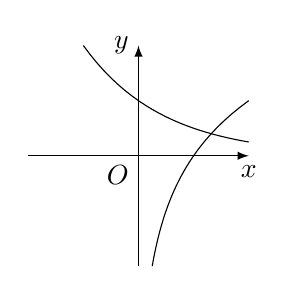
\begin{tikzpicture}[scale = 0.7, >=latex]
    \draw [->] (-2,0) -- (2,0) node [below] {$x$};
    \draw [->] (0,-2) -- (0,2) node [left] {$y$};
    \draw (0,0) node [below left] {$O$};
    \draw [domain = -1:2] plot (\x, {pow(0.5,\x)});
    \draw [domain = -1:2] plot ({pow(0.5,\x)},-\x);
\end{tikzpicture}}
{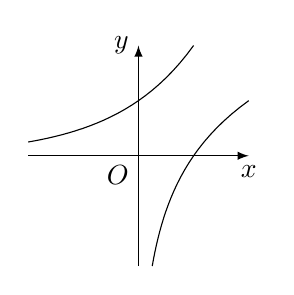
\begin{tikzpicture}[scale = 0.7, >=latex]
    \draw [->] (-2,0) -- (2,0) node [below] {$x$};
    \draw [->] (0,-2) -- (0,2) node [left] {$y$};
    \draw (0,0) node [below left] {$O$};
    \draw [domain = -1:2] plot (-\x, {pow(0.5,\x)});
    \draw [domain = -1:2] plot ({pow(0.5,\x)},-\x);
\end{tikzpicture}}{\begin{tikzpicture}[scale = 0.7, >=latex]
    \draw [->] (-2,0) -- (2,0) node [below] {$x$};
    \draw [->] (0,-2) -- (0,2) node [left] {$y$};
    \draw (0,0) node [below left] {$O$};
    \draw [domain = -1:2] plot (-\x, {pow(0.5,\x)});
    \draw [domain = -1:2] plot ({pow(0.5,\x)},\x);
\end{tikzpicture}}{\begin{tikzpicture}[scale = 0.7, >=latex]
    \draw [->] (-2,0) -- (2,0) node [below] {$x$};
    \draw [->] (0,-2) -- (0,2) node [left] {$y$};
    \draw (0,0) node [below left] {$O$};
    \draw [domain = -1:2] plot (\x, {pow(0.5,\x)});
    \draw [domain = -1:2] plot ({pow(0.5,\x)},\x);
\end{tikzpicture}}


关联目标:

暂未关联目标



标签: 第二单元

答案: 暂无答案

解答或提示: 暂无解答与提示

使用记录:

暂无使用记录


出处: 二期课改练习册高一第二学期
\item { (008095)}函数$f(x)=4+\log _a(x-1)(a>0a\ne 1)$的图像恒经过定点$P$, 则点$P$的坐标是\bracket{20}.
\fourch{$(1, 4)$}{($4, 1)$}{$(2, 4)$}{$(4, 2)$}


关联目标:

暂未关联目标



标签: 第二单元

答案: 暂无答案

解答或提示: 暂无解答与提示

使用记录:

暂无使用记录


出处: 二期课改练习册高一第二学期
\item { (008096)}已知$0<a<1$, 化简$\sqrt {\lg ^2a-\lg \dfrac{a^2}{10}}$.


关联目标:

暂未关联目标



标签: 第二单元

答案: 暂无答案

解答或提示: 暂无解答与提示

使用记录:

暂无使用记录


出处: 二期课改练习册高一第二学期
\item { (008097)}已知$\alpha$、$\beta$是方程$\lg ^2x-\lg x-2=0$的两根, 求$\log _{\alpha }\beta +\log _{\beta }\alpha$的值.


关联目标:

暂未关联目标



标签: 第二单元

答案: 暂无答案

解答或提示: 暂无解答与提示

使用记录:

暂无使用记录


出处: 二期课改练习册高一第二学期
\item { (008363)}如果已知$f(x)=2^{-x}$, 则$f(\log _23)=$\blank{50}.


关联目标:

暂未关联目标



标签: 第二单元

答案: 暂无答案

解答或提示: 暂无解答与提示

使用记录:

暂无使用记录


出处: 二期课改练习册高一第二学期
\item { (008365)}若$\log _x\dfrac 45<1$, 则$x$的取值范围为\blank{50}.


关联目标:

暂未关联目标



标签: 第二单元

答案: 暂无答案

解答或提示: 暂无解答与提示

使用记录:

暂无使用记录


出处: 二期课改练习册高一第二学期
\item { (008366)}函数$y=\dfrac 1{\sqrt {\log _{\frac 12}(2-x)}}$的定义域是\blank{50}.


关联目标:

暂未关联目标



标签: 第二单元

答案: 暂无答案

解答或提示: 暂无解答与提示

使用记录:

暂无使用记录


出处: 二期课改练习册高一第二学期
\item { (008371)}在同一坐标系内作出的两个函数图像如图所示, 这两个函数为\bracket{20}.
\begin{center}
    \begin{tikzpicture}[>=latex]
        \draw [->] (-2,0) -- (2,0) node [below] {$x$};
        \draw [->] (0,-2) -- (0,2) node [left] {$y$};
        \draw (0,0) node [below left] {$O$};
        \draw [domain = -1:2] plot (\x,{pow(2,-\x)});
        \draw [domain = -1:2] plot ({-pow(2,-\x)},-\x);
        \draw (0,1) node [above right] {$1$};
        \draw (-1,0) node [below left] {$-1$};
    \end{tikzpicture}
\end{center}
\twoch{$y=a^x$和$y=\log _a(-x)$}{$y=a^x$和$y=\log _ax^{-1}$}{$y=a^{-x}$和$y=\log _ax^{-1}$}{$y=a^{-x}$和$y=\log _a(-x)$}


关联目标:

暂未关联目标



标签: 第二单元

答案: 暂无答案

解答或提示: 暂无解答与提示

使用记录:

暂无使用记录


出处: 二期课改练习册高一第二学期
\item { (008372)}若$0<x<\dfrac{\pi}4$, 且$\lg (\sin x+\cos x)=\dfrac 12(3\lg 2-\lg 5)$, 则$\cos x-\sin x$的值为\bracket{20}.
\fourch{$\dfrac{\sqrt 6}3$}{$\dfrac{\sqrt 3}2$}{$\dfrac{\sqrt {10}}5$}{$\dfrac{\sqrt 5}4$}


关联目标:

暂未关联目标



标签: 第三单元|第二单元

答案: 暂无答案

解答或提示: 暂无解答与提示

使用记录:

暂无使用记录


出处: 二期课改练习册高一第二学期
\item { (008375)}解方程: $\log _3(x-1)=\log _9(x+5)$.


关联目标:

暂未关联目标



标签: 第二单元

答案: 暂无答案

解答或提示: 暂无解答与提示

使用记录:

暂无使用记录


出处: 二期课改练习册高一第二学期
\item { (008376)}解方程: $\log _2(9^x-5)=\log _2(3^x-2)+2$.


关联目标:

暂未关联目标



标签: 第二单元

答案: 暂无答案

解答或提示: 暂无解答与提示

使用记录:

暂无使用记录


出处: 二期课改练习册高一第二学期
\item { (008378)}已知函数$f(x)=\log _2(2^x-1)$.\\
(1) 求$f(x)$的定义域;\\
(2) 判断$f(x)$的增减性, 说明理由;\\
(3) 求$f^{-1}(x)$.


关联目标:

暂未关联目标



标签: 第二单元

答案: 暂无答案

解答或提示: 暂无解答与提示

使用记录:

暂无使用记录


出处: 二期课改练习册高一第二学期
\item { (008388)}若$\log_m 3<\log_n 3<0$, 则$m,n$满足的条件是\bracket{20}.
\fourch{$m>n>1$}{$n>m>1$}{$0<m<n<1$}{$0<n<m<1$}


关联目标:

暂未关联目标



标签: 第二单元

答案: 暂无答案

解答或提示: 暂无解答与提示

使用记录:

暂无使用记录


出处: 二期课改练习册高一第二学期
\item { (008389)}若$\log _3x=\cos x$解的个数有\bracket{20}.
\fourch{$0$}{$1$}{$2$}{$3$}


关联目标:

暂未关联目标



标签: 第三单元|第二单元

答案: 暂无答案

解答或提示: 暂无解答与提示

使用记录:

暂无使用记录


出处: 二期课改练习册高一第二学期
\item { (008391)}若$\lg a\lg b$是方程$2x^2-4x+1=0$的两个根, 则$(\lg \dfrac ab)^2$的值等于\blank{50}.


关联目标:

暂未关联目标



标签: 第二单元

答案: 暂无答案

解答或提示: 暂无解答与提示

使用记录:

暂无使用记录


出处: 二期课改练习册高一第二学期
\item { (008392)}定义在$\mathbf{R}$上的偶函数$f(x)$在$[0,+\infty)$上是增函数, 且$f(\dfrac 12)=0$, 则满足$f(\log _{\dfrac 14}x)>0$的$x$的值范围是\blank{50}.


关联目标:

暂未关联目标



标签: 第二单元

答案: 暂无答案

解答或提示: 暂无解答与提示

使用记录:

暂无使用记录


出处: 二期课改练习册高一第二学期
\item { (008394)}已知函数$f(x)=\log _a\dfrac{x+b}{x-b}(a>0,b>0, a\ne 1)$.\\
(1) 求$f(x)$的定义域;\\
(2) 判断$f(x)$的奇偶性;\\
(3) 求函数$y=f^{-1}(x)$的解析式.


关联目标:

暂未关联目标



标签: 第二单元

答案: 暂无答案

解答或提示: 暂无解答与提示

使用记录:

暂无使用记录


出处: 二期课改练习册高一第二学期
\item { (009473)}用有理数指数幂的形式表示下列各式(其中$a>0$):\\
(1) $a^{\frac{10}3}\cdot \sqrt[5]{a^3}$;\\
(2) $\sqrt[3]{a\sqrt[3]{a}}$.


关联目标:

暂未关联目标



标签: 第二单元

答案: 暂无答案

解答或提示: 暂无解答与提示

使用记录:

暂无使用记录


出处: 新教材必修第一册课堂练习
\item { (009476)}以下对数式中, 与指数式$5^x=6$等价的是\bracket{20}.
\fourch{$\log_56=x$}{$\log_5x=6$}{$\log_6x=5$}{$\log_x6=5$}


关联目标:

暂未关联目标



标签: 第二单元

答案: 暂无答案

解答或提示: 暂无解答与提示

使用记录:

暂无使用记录


出处: 新教材必修第一册课堂练习
\item { (009477)}求下列各式的值:\\
(1) $\log_525$;\\
(2) $\log_{\frac 13}27$;\\
(3) $\log_4\sqrt 2$;\\
(4) $2^{\log_23}$.


关联目标:

暂未关联目标



标签: 第二单元

答案: 暂无答案

解答或提示: 暂无解答与提示

使用记录:

暂无使用记录


出处: 新教材必修第一册课堂练习
\item { (009478)}求下列各式中$x$的值:\\
(1) $\log_4x=2$;\\
(2) $\log_x4=2$.


关联目标:

暂未关联目标



标签: 第二单元

答案: 暂无答案

解答或提示: 暂无解答与提示

使用记录:

暂无使用记录


出处: 新教材必修第一册课堂练习
\item { (009479)}已知$A=\log_ax$, $B=\log_ay$($a>0$且$a\ne 1$). 用$A$及$B$表示下列各式:\\
(1) $\log_axy$;\\
(2) $\log_ax^2\sqrt y$.


关联目标:

暂未关联目标



标签: 第二单元

答案: 暂无答案

解答或提示: 暂无解答与提示

使用记录:

暂无使用记录


出处: 新教材必修第一册课堂练习
\item { (009480)}求下列各式的值:\\
(1) $\log_{15}3+\log_{15}5$;\\
(2) $\log_2\sqrt[3]{4}$;\\
(3) $\log_5\sqrt{10}-\dfrac 12\log_5250$.


关联目标:

暂未关联目标



标签: 第二单元

答案: 暂无答案

解答或提示: 暂无解答与提示

使用记录:

暂无使用记录


出处: 新教材必修第一册课堂练习
\item { (009481)}已知$\log_73=a$, $7^b=2$. 用$a$及$b$表示$\log_772$.


关联目标:

暂未关联目标



标签: 第二单元

答案: 暂无答案

解答或提示: 暂无解答与提示

使用记录:

暂无使用记录


出处: 新教材必修第一册课堂练习
\item { (009482)}求下列各式的值:\\
(1) $\log_8\dfrac 14$;\\
(2) $\log_ab\cdot\log_bc\cdot\log_ca$($a$、$b$、$c$均为不等于$1$的正数);\\
(3) $3^{2+\log_94}$;\\
(4) $\dfrac{\log_52\times\log_79}{\log_5\dfrac 13\times\log_72}$.


关联目标:

暂未关联目标



标签: 第二单元

答案: 暂无答案

解答或提示: 暂无解答与提示

使用记录:

暂无使用记录


出处: 新教材必修第一册课堂练习
\item { (009483)}已知$\log_32=a$, 用$a$表示$\log_296$.


关联目标:

暂未关联目标



标签: 第二单元

答案: 暂无答案

解答或提示: 暂无解答与提示

使用记录:

暂无使用记录


出处: 新教材必修第一册课堂练习
\item { (009484)}设$a$、$b$是两个不等于$1$的正数, 求证: $\log_ba=\dfrac1{\log_ab}$.


关联目标:

暂未关联目标



标签: 第二单元

答案: 暂无答案

解答或提示: 暂无解答与提示

使用记录:

暂无使用记录


出处: 新教材必修第一册课堂练习
\item { (009485)}若幂函数$y=x^a$的图像经过点$(3, \sqrt 3)$, 求此幂函数的表达式.


关联目标:

暂未关联目标



标签: 第二单元

答案: 暂无答案

解答或提示: 暂无解答与提示

使用记录:

暂无使用记录


出处: 新教材必修第一册课堂练习
\item { (009487)}若幂函数$y=x^{-m^2+2m+3}$($m$为整数)的定义域为$\mathbf{R}$, 求$m$的值.


关联目标:

暂未关联目标



标签: 第二单元

答案: 暂无答案

解答或提示: 暂无解答与提示

使用记录:

暂无使用记录


出处: 新教材必修第一册课堂练习
\item { (009491)}判断下列函数哪些是指数函数, 哪些是幂函数:\\
(1) $y=x$;\\
(2) $y=x^3$;\\
(3) $y=\mathrm{e}^x$;\\
(4) $y=\sqrt[3]{x}$;\\
(5) $y=2^{-x}$;\\
(6) $y=2^x$.


关联目标:

暂未关联目标



标签: 第二单元

答案: 暂无答案

解答或提示: 暂无解答与提示

使用记录:

暂无使用记录


出处: 新教材必修第一册课堂练习
\item { (009492)}求下列函数的定义域:\\
(1) $y=3^x$;\\
(2) $y=3^{\frac 1{x-2}}$.


关联目标:

暂未关联目标



标签: 第二单元

答案: 暂无答案

解答或提示: 暂无解答与提示

使用记录:

暂无使用记录


出处: 新教材必修第一册课堂练习
\item { (009493)}在同一平面直角坐标系中分别作出下列函数的大致图像:\\
(1) $y=4^x$;\\
(2) $y=(\dfrac 14)^x$.


关联目标:

暂未关联目标



标签: 第二单元

答案: 暂无答案

解答或提示: 暂无解答与提示

使用记录:

暂无使用记录


出处: 新教材必修第一册课堂练习
\item { (009495)}已知$a>0$且$a\ne 1$. 若$m>n$, 且$a^m<a^n$, 求实数$a$的取值范围.


关联目标:

暂未关联目标



标签: 第二单元

答案: 暂无答案

解答或提示: 暂无解答与提示

使用记录:

暂无使用记录


出处: 新教材必修第一册课堂练习
\item { (009496)}求下列不等式的解集:\\
(1) $3^x>3^{0.5}$;\\
(2) $0.2^x<25$.


关联目标:

暂未关联目标



标签: 第二单元

答案: 暂无答案

解答或提示: 暂无解答与提示

使用记录:

暂无使用记录


出处: 新教材必修第一册课堂练习
\item { (009497)}已知指数函数$y=a^x$($0<a<1$)在区间$[1, 2]$上的最大值比最小值大$\dfrac a3$, 求实数$a$的值.


关联目标:

暂未关联目标



标签: 第二单元

答案: 暂无答案

解答或提示: 暂无解答与提示

使用记录:

暂无使用记录


出处: 新教材必修第一册课堂练习
\item { (009499)}若对数函数$y=\log a_x$($a>0$且$a\ne 1$)的图像经过点$(4, 2)$, 求此对数函数的表达式.


关联目标:

暂未关联目标



标签: 第二单元

答案: 暂无答案

解答或提示: 暂无解答与提示

使用记录:

暂无使用记录


出处: 新教材必修第一册课堂练习
\item { (009500)}求下列函数的定义域:\\
(1) $y=\log_2\dfrac{2+x}{1-x}$;\\
(2) $y=\log_a(4-x^2)$(常数$a>0$且$a\ne 1$).


关联目标:

暂未关联目标



标签: 第二单元

答案: 暂无答案

解答或提示: 暂无解答与提示

使用记录:

暂无使用记录


出处: 新教材必修第一册课堂练习
\item { (009501)}在同一平面直角坐标系中作出$y=\lg x$及$y=\log_{0.1}x$的大致图像.


关联目标:

暂未关联目标



标签: 第二单元

答案: 暂无答案

解答或提示: 暂无解答与提示

使用记录:

暂无使用记录


出处: 新教材必修第一册课堂练习
\item { (009502)}已知常数$a>0$且$a\ne 1$, 假设无论$a$取何值, 函数$y=\log_a(x-1)$的图像恒经过一个定点, 求此点的坐标.


关联目标:

暂未关联目标



标签: 第二单元

答案: 暂无答案

解答或提示: 暂无解答与提示

使用记录:

暂无使用记录


出处: 新教材必修第一册课堂练习
\item { (009503)}利用对数函数的性质, 比较下列各题中两个对数的大小:\\
(1) $\log_{0.2}3$和$\log_{0.2}6$;\\
(2) $\log_{0.2}3$和$\log_{0.3}3$.


关联目标:

暂未关联目标



标签: 第二单元

答案: 暂无答案

解答或提示: 暂无解答与提示

使用记录:

暂无使用记录


出处: 新教材必修第一册课堂练习
\item { (009504)}设$0<a<1$, 求证: 对数函数$y=\log_ax$在区间$(0, +\infty)$上是严格减函数.


关联目标:

暂未关联目标



标签: 第二单元

答案: 暂无答案

解答或提示: 暂无解答与提示

使用记录:

暂无使用记录


出处: 新教材必修第一册课堂练习
\item { (009506)}利用对数函数的单调性来估算对数$\log_25$的第一位小数的值.


关联目标:

暂未关联目标



标签: 第二单元

答案: 暂无答案

解答或提示: 暂无解答与提示

使用记录:

暂无使用记录


出处: 新教材必修第一册课堂练习
\item { (009508)}下列四组函数中, 同组的两个函数是相同函数的是\bracket{20}.
\twoch{$y=|x|$与$y=(\sqrt x)^2$}{$y=x$与$y=\mathrm{e}^{\ln x}$}{$y=x$与$y=\sqrt[5]{x^5}$}{$y=x$与$y=(\dfrac 1x)^{-1}$}


关联目标:

暂未关联目标



标签: 第二单元

答案: 暂无答案

解答或提示: 暂无解答与提示

使用记录:

暂无使用记录


出处: 新教材必修第一册课堂练习
\item { (009509)}求下列函数的值域:\\
(1) $y=(\lg x)^2+1$, $x\in (0, +\infty)$;\\
(2) $y=3x^2-4x+1$, $x\in [0, 1]$.


关联目标:

暂未关联目标



标签: 第二单元

答案: 暂无答案

解答或提示: 暂无解答与提示

使用记录:

暂无使用记录


出处: 新教材必修第一册课堂练习
\item { (009514)}证明下列函数是奇函数:\\
(1) $y=2^x-2^{-x}$;\\
(2) $y=\log_2(1+x)-\log_2(1-x)$.


关联目标:

暂未关联目标



标签: 第二单元

答案: 暂无答案

解答或提示: 暂无解答与提示

使用记录:

暂无使用记录


出处: 新教材必修第一册课堂练习
\item { (009523)}求函数$y=(\dfrac 12)^x$, $x\in [1, 3]$的最大值与最小值.


关联目标:

暂未关联目标



标签: 第二单元

答案: 暂无答案

解答或提示: 暂无解答与提示

使用记录:

暂无使用记录


出处: 新教材必修第一册课堂练习
\item { (009530)}用函数的观点解不等式: $2^x+\log_2x>2$.


关联目标:

暂未关联目标



标签: 第二单元

答案: 暂无答案

解答或提示: 暂无解答与提示

使用记录:

暂无使用记录


出处: 新教材必修第一册课堂练习
\item { (009908)}借助函数图像, 判断下列导数的正负(可利用信息技术工具):\\
(1) $f'(\dfrac\pi 4)$, 其中$f(x)=\sin x$;\\
(2) $f'(0)$, 其中$f(x)=(\dfrac 12)^x$.


关联目标:

暂未关联目标



标签: 第二单元

答案: 暂无答案

解答或提示: 暂无解答与提示

使用记录:

暂无使用记录


出处: 新教材选择性必修第二册课堂练习
\item { (009912)}证明函数$y=\ln x$与$y=\mathrm{e}^x$没有驻点.


关联目标:

暂未关联目标



标签: 第二单元

答案: 暂无答案

解答或提示: 暂无解答与提示

使用记录:

暂无使用记录


出处: 新教材选择性必修第二册课堂练习
\item { (009913)}求下列函数$y=f(x)$的导数, 其中:\\
(1) $f(x)=3\mathrm{e}^x-x^{\mathrm{e}}+\mathrm{e}$;\\
(2) $f(x)=\cos x-\dfrac 2x$;\\
(3) $f(x)=(2x+1)^3$;\\
(4) $f(x)=\sqrt x\sin x$;\\
(5) $f(x)=x\ln x-\dfrac1{x^2}$;\\
(6) $f(x)=\dfrac{x^2-1}x$;\\
(7) $f(x)=\dfrac{x^2-1}{x^2+1}$;\\
(8) $f(x)=\tan x$.


关联目标:

暂未关联目标



标签: 第二单元

答案: 暂无答案

解答或提示: 暂无解答与提示

使用记录:

暂无使用记录


出处: 新教材选择性必修第二册课堂练习
\item { (009917)}求下列函数的导数:\\
(1) $y=3x \sqrt{2-x}$;\\
(2) $y=\dfrac{\ln(2x+1)}x$.


关联目标:

暂未关联目标



标签: 第二单元

答案: 暂无答案

解答或提示: 暂无解答与提示

使用记录:

暂无使用记录


出处: 新教材选择性必修第二册课堂练习
\item { (009918)}利用导数研究下列函数的单调性, 并说明所得结果与你之前的认识是否一致:\\
(1) $y=\mathrm{e}^x$;\\
(2) $y=\ln x$;\\
(3) $y=ax^2+bx+c$, 其中$a\ne 0$.


关联目标:

暂未关联目标



标签: 第二单元

答案: 暂无答案

解答或提示: 暂无解答与提示

使用记录:

暂无使用记录


出处: 新教材选择性必修第二册课堂练习
\item { (009919)}确定下列函数的单调区间:\\
(1) $y=x\mathrm{e}^x$;\\
(2) $y=4x^3-9x^2+6x+7$.


关联目标:

暂未关联目标



标签: 第二单元

答案: 暂无答案

解答或提示: 暂无解答与提示

使用记录:

暂无使用记录


出处: 新教材选择性必修第二册课堂练习
\item { (010001)}已知$f(x)=\log_3(x+a)+\log_3(6-x)$.\\
(1) 若将函数$y=f(x)$的图像向下平移$m$($m>0$)个单位后, 所得的图像经过点$(3,0)$与点$(5,0)$, 求$a$与$m$的值;\\
(2) 若$a>-3$且$a\ne 0$, 解关于$x$的不等式$f(x)\le f(6-x)$.


关联目标:

暂未关联目标



标签: 第二单元

答案: 暂无答案

解答或提示: 暂无解答与提示

使用记录:

暂无使用记录


出处: 上海2022年秋季高考试题18
\item { (010107)}用有理数指数幂的形式表示下列各式(其中$x>0$, $y>0$):\\
(1) $\sqrt[3]{5}$;\\
(2) $(\sqrt[5]{x})^3$;\\
(3) $\sqrt[7]{x^3y^4}$;\\
(4) $\sqrt[7]{\dfrac{x^3}{y^4}}$.


关联目标:

暂未关联目标



标签: 第二单元

答案: 暂无答案

解答或提示: 暂无解答与提示

使用记录:

暂无使用记录


出处: 新教材必修第一册习题
\item { (010110)}用有理数指数幂的形式表示下列各式(其中$a>0$, $b>0$):\\
(1) $a^\frac 13a^\frac 14$;\\
(2) $\sqrt[3]{a\sqrt a}$;\\
(3) $(a^\frac 14b^{-\frac 38})^8$;\\
(4) $(\dfrac {a^{-3}b^4}{\sqrt b})^{-\frac 13}$.


关联目标:

暂未关联目标



标签: 第二单元

答案: 暂无答案

解答或提示: 暂无解答与提示

使用记录:

暂无使用记录


出处: 新教材必修第一册习题
\item { (010113)}设$a^{2x}=2$, 且$a>0$. 求$\dfrac{a^{3x}+a^{-3x}}{a^x+a^{-x}}$的值.


关联目标:

暂未关联目标



标签: 第二单元

答案: 暂无答案

解答或提示: 暂无解答与提示

使用记录:

暂无使用记录


出处: 新教材必修第一册习题
\item { (010114)}设$a>b>0$, 求证: $a^ab^b>(ab)^\frac{a+b}2$.


关联目标:

暂未关联目标



标签: 第二单元

答案: 暂无答案

解答或提示: 暂无解答与提示

使用记录:

暂无使用记录


出处: 新教材必修第一册习题
\item { (010115)}把下列指数式写成对数式:\\
(1) $3^4=81$;\\
(2) $5^{-\frac1 2}=x$.


关联目标:

暂未关联目标



标签: 第二单元

答案: 暂无答案

解答或提示: 暂无解答与提示

使用记录:

暂无使用记录


出处: 新教材必修第一册习题
\item { (010116)}将下列对数式写成指数式:\\
(1) $\log_{\frac 13}27=-3$;\\
(2) $\log_2\dfrac 18=-3$.


关联目标:

暂未关联目标



标签: 第二单元

答案: 暂无答案

解答或提示: 暂无解答与提示

使用记录:

暂无使用记录


出处: 新教材必修第一册习题
\item { (010117)}求下列各式的值:\\
(1) $\log_3 27$;\\
(2) $\log_{\frac 12}8$;\\
(3) $\ln \dfrac 1{\mathrm{e}}+\lg \sqrt {10}$.


关联目标:

暂未关联目标



标签: 第二单元

答案: 暂无答案

解答或提示: 暂无解答与提示

使用记录:

暂无使用记录


出处: 新教材必修第一册习题
\item { (010118)}求下列各式中$x$的值:\\
(1) $\log_2x=5$;\\
(2) $\log_{\sqrt 5}\dfrac1{125}=x$;\\
(3) $\log_x4=\dfrac 12$.


关联目标:

暂未关联目标



标签: 第二单元

答案: 暂无答案

解答或提示: 暂无解答与提示

使用记录:

暂无使用记录


出处: 新教材必修第一册习题
\item { (010119)}求下列各式的值:\\
(1) $\log_2(2\times 3\sqrt 2)$;\\
(2) $\log_{21}3+\log_{21}7$;\\
(3) $\log_5\sqrt 6-\dfrac 12\log_5 150$;\\
(4) $3^{\log_31}+\log_248-\log_23$;\\
(5) $3\log_3\dfrac 32-\log_3\dfrac 74+\dfrac 12\log_34+\log_37$.


关联目标:

暂未关联目标



标签: 第二单元

答案: 暂无答案

解答或提示: 暂无解答与提示

使用记录:

暂无使用记录


出处: 新教材必修第一册习题
\item { (010120)}已知$A=\log_ax$, $B=\log_ay$, $C=\log_az$($a>0$且$a\ne 1)$. 用$A$、$B$及$C$表示下列各式:\\
(1) $\log_a(xy^2)$;\\
(2) $\log_a\dfrac{xy}{\sqrt z}$;\\
(3) $\log_a(x^2y^2)+\log_a(y\sqrt x)$.


关联目标:

暂未关联目标



标签: 第二单元

答案: 暂无答案

解答或提示: 暂无解答与提示

使用记录:

暂无使用记录


出处: 新教材必修第一册习题
\item { (010121)}求下列各式的值:\\
(1) $\log_42\sqrt 2$;\\
(2) $\log_23\times \log_92$;\\
(3) $\dfrac 3{\log_26}+\dfrac 3{\log_36}$;\\
(4) $(\log_43+\log_83)(\log_32+\log_92)+\log_{\frac 12}\sqrt[4]{32}$.


关联目标:

暂未关联目标



标签: 第二单元

答案: 暂无答案

解答或提示: 暂无解答与提示

使用记录:

暂无使用记录


出处: 新教材必修第一册习题
\item { (010122)}已知$a=\lg 5$, 用$a$表示$\lg 2$和$\lg$ $20$.


关联目标:

暂未关联目标



标签: 第二单元

答案: 暂无答案

解答或提示: 暂无解答与提示

使用记录:

暂无使用记录


出处: 新教材必修第一册习题
\item { (010123)}求下列各式中$x$的取值范围:\\
(1) $\log_2(1-3x)$;\\
(2) $\log_a(x^2+x)$($a>0$且$a\ne 1)$.


关联目标:

暂未关联目标



标签: 第二单元

答案: 暂无答案

解答或提示: 暂无解答与提示

使用记录:

暂无使用记录


出处: 新教材必修第一册习题
\item { (010124)}求下列各式的值:\\
(1) $\log_48-\log_{\frac 19}3-\log_{\sqrt 2}4$;\\
(2) $2^{\log_65}\times 3^{\log_65}$;\\
(3) $(\lg 50)^2+\lg 2\times \lg 50^2+(\lg 2)^2$.


关联目标:

暂未关联目标



标签: 第二单元

答案: 暂无答案

解答或提示: 暂无解答与提示

使用记录:

暂无使用记录


出处: 新教材必修第一册习题
\item { (010125)}科学家以里氏震级来度量地震的强度, 若设$I$为地震时所散发出来的相对能量程度, 则里氏震级度量$r$可定义为$r=\dfrac 23\lg I+2$. 求$7.8$级地震和$6. 9$级地震的相对能量比值. (结果精确到个位)


关联目标:

暂未关联目标



标签: 第二单元

答案: 暂无答案

解答或提示: 暂无解答与提示

使用记录:

暂无使用记录


出处: 新教材必修第一册习题
\item { (010126)}已知$\lg 2=a$, $\lg 3=b$. 用$a$及$b$表示$\log_2 3$及$\log_{12}25$.


关联目标:

暂未关联目标



标签: 第二单元

答案: 暂无答案

解答或提示: 暂无解答与提示

使用记录:

暂无使用记录


出处: 新教材必修第一册习题
\item { (010127)}已知$5.4^x=3$, $0.6^y=3$. 求$\dfrac 1x-\dfrac 1y$的值.


关联目标:

暂未关联目标



标签: 第二单元

答案: 暂无答案

解答或提示: 暂无解答与提示

使用记录:

暂无使用记录


出处: 新教材必修第一册习题
\item { (010128)}设$a$、$b$、$c$、$d$均为正数, 且$a$、$c$均不为$1$. 求证:
$\log_ab\cdot \log_cd=\log_ad\cdot \log_cb$.


关联目标:

暂未关联目标



标签: 第二单元

答案: 暂无答案

解答或提示: 暂无解答与提示

使用记录:

暂无使用记录


出处: 新教材必修第一册习题
\item { (010129)}若幂函数$y=x^a$的图像经过点$(\sqrt[4]{3}, 3)$, 求此幂函数的表达式.


关联目标:

暂未关联目标



标签: 第二单元

答案: 暂无答案

解答或提示: 暂无解答与提示

使用记录:

暂无使用记录


出处: 新教材必修第一册习题
\item { (010133)}下列幂函数在区间$(0, +\infty)$上是严格增函数, 且图像关于原点成中心对称的是\blank{50}(请填入全部正确的序号).\\
\textcircled{1} $y=x^\frac 12$; \textcircled{2} $y=x^\frac 13$; \textcircled{3} $y=x^\frac 23$; \textcircled{4} $y=x^{-\frac 13}$.


关联目标:

暂未关联目标



标签: 第二单元

答案: 暂无答案

解答或提示: 暂无解答与提示

使用记录:

暂无使用记录


出处: 新教材必修第一册习题
\item { (010135)}幂函数$y=x^{n(n+1)}$($n$为正整数)的图像一定经过\blank{50}象限.


关联目标:

暂未关联目标



标签: 第二单元

答案: 暂无答案

解答或提示: 暂无解答与提示

使用记录:

暂无使用记录


出处: 新教材必修第一册习题
\item { (010136)}若幂函数$y=x^s$在$0<x<1$时的图像位于直线$y=x$的上方, 则$s$的取值范围是\blank{50}.


关联目标:

暂未关联目标



标签: 第二单元

答案: 暂无答案

解答或提示: 暂无解答与提示

使用记录:

暂无使用记录


出处: 新教材必修第一册习题
\item { (010137)}下列命题中, 正确的是\bracket{20}.
\onech{当$n=0$时, 函数$y=x^n$的图像是一条直线}{幂函数$y=x^n$的图像都经过$(0, 0)$和$(1, 1)$两个点}{若幂函数$y=x^n$的图像关于原点成中心对称, 则$y=x^n$在区间$(-\infty, 0)$上是严格增函数}{幂函数的图像不可能在第四象限}


关联目标:

暂未关联目标



标签: 第二单元

答案: 暂无答案

解答或提示: 暂无解答与提示

使用记录:

暂无使用记录


出处: 新教材必修第一册习题
\item { (010138)}写出一个图像经过第一、第二象限但不经过原点的幂函数的表达式.


关联目标:

暂未关联目标



标签: 第二单元

答案: 暂无答案

解答或提示: 暂无解答与提示

使用记录:

暂无使用记录


出处: 新教材必修第一册习题
\item { (010140)}下列函数是指数函数的序号为\blank{50}(请填入全部正确的序号).\\
\textcircled{1} $y=(-4)^x$; \textcircled{2} $y=(\dfrac 14)^x$; \textcircled{3} $y=4^x$; \textcircled{4} $y=x^{-4}$; \textcircled{5} $y=(\sqrt 4)^x$.


关联目标:

暂未关联目标



标签: 第二单元

答案: 暂无答案

解答或提示: 暂无解答与提示

使用记录:

暂无使用记录


出处: 新教材必修第一册习题
\item { (010142)}在同一直角坐标系中作出下列函数的大致图像, 并指出这些函数图像间的关系:\\
(1) $y=(\dfrac 32)^x$;\\
(2) $y=(\dfrac 23)^x$;\\
(3) $y=(\dfrac 23)^x-1$.


关联目标:

暂未关联目标



标签: 第二单元

答案: 暂无答案

解答或提示: 暂无解答与提示

使用记录:

暂无使用记录


出处: 新教材必修第一册习题
\item { (010143)}已知指数函数$y=(m-2)^x$在$\mathbf{R}$上是严格减函数, 求实数$m$的取值范围.


关联目标:

暂未关联目标



标签: 第二单元

答案: 暂无答案

解答或提示: 暂无解答与提示

使用记录:

暂无使用记录


出处: 新教材必修第一册习题
\item { (010147)}已知指数函数$y=a^x$($a>0$且$a\ne 1)$在区间$[1, 2]$上的最大值与最小值之和等于$6$, 求实数$a$的值.


关联目标:

暂未关联目标



标签: 第二单元

答案: 暂无答案

解答或提示: 暂无解答与提示

使用记录:

暂无使用记录


出处: 新教材必修第一册习题
\item { (010149)}在同一平面直角坐标系中, 指数函数$y=a^x$($a>0$且$a\ne 1$)和一次函数$y=a(x+1)$的图像关系可能是\bracket{20}.
\fourch{\begin{tikzpicture}[>=latex,scale=0.7]
\draw [->] (-2,0) -- (2,0) node [below] {$x$};
\draw [->] (0,-1) -- (0,2.5) node [left] {$y$};
\draw (0,0) node [below left] {$O$};
\draw [domain = -2:1.3] plot (-\x,{pow(2,\x)});
\draw (-1.5,-1) -- (0.25,2.5);
\draw (0.2,1) -- (0,1) node [below left] {$1$};
\draw (-1,0.2) -- (-1,0) node [above left] {$-1$};
\end{tikzpicture}}{\begin{tikzpicture}[>=latex,scale=0.7]
\draw [->] (-2,0) -- (2,0) node [below] {$x$};
\draw [->] (0,-1) -- (0,2.5) node [left] {$y$};
\draw (0,0) node [below left] {$O$};
\draw [domain = -2:1.3] plot (-\x,{pow(2,\x)});
\draw (-1,-1) -- (2,0.5);
\draw (0.2,1) -- (0,1) node [below left] {$1$};
\draw (1,0.2) -- (1,0) node [below] {$1$};
\end{tikzpicture}}{\begin{tikzpicture}[>=latex,scale=0.7]
\draw [->] (-2,0) -- (2,0) node [below] {$x$};
\draw [->] (0,-1) -- (0,2.5) node [left] {$y$};
\draw (0,0) node [below left] {$O$};
\draw [domain = -2:1.3] plot (\x,{pow(2,\x)});
\draw (-1.5,-1) -- (0.25,2.5);
\draw (0.2,1) -- (0,1) node [below right] {$1$};
\draw (-1,0.2) -- (-1,0) node [below left] {$-1$};
\end{tikzpicture}}{\begin{tikzpicture}[>=latex,scale=0.7]
\draw [->] (-2,0) -- (2,0) node [below] {$x$};
\draw [->] (0,-1) -- (0,2.5) node [left] {$y$};
\draw (0,0) node [below left] {$O$};
\draw [domain = -2:1.3] plot (\x,{pow(2,\x)});
\draw (-2,-0.5) -- (2,1.5);
\draw (0.2,1) -- (0,1) node [above left] {$1$};
\draw (-1,0.2) -- (-1,0) node [below] {$-1$};
\end{tikzpicture}}


关联目标:

暂未关联目标



标签: 第二单元

答案: 暂无答案

解答或提示: 暂无解答与提示

使用记录:

暂无使用记录


出处: 新教材必修第一册习题
\item { (010150)}如图所示的是某池塘中的浮萍蔓延的面积$y$(单位: $\text{m}^2$)与时间$t$(单位: 月)的关系: $y=a^t$($a>0$且$a\ne 1)$. 
\begin{center}
\begin{tikzpicture}[>=latex,scale = 0.5]
\draw [->] (0,0) -- (4,0) node [below] {$t/\text{月}$};
\draw [->] (0,0) -- (0,9) node [left] {$y/\text{m}^2$};
\draw (0,0) node [below left] {$O$};
\draw [domain = 0:3.1] plot (\x,{pow(2,\x)});
\foreach \i in {1,2,3}{\draw [dashed] (\i,0) -- (\i,{pow(2,\i)}) -- (0,{pow(2,\i)}); \draw (\i,0) node [below] {$\i$};};
\foreach \i in {2,4,8}{\draw (0,\i) node [left] {$\i$};};
\end{tikzpicture}
\end{center}
以下结论:
\textcircled{1} 这个指数函数的底数是$2$; 
\textcircled{2} 第$5$个月时, 浮萍的面积就会超过$30\text{m}^2$;
\textcircled{3} 浮萍面积从$4\text{m}^2$到$12\text{m}^2$需要经过$1.5$个月;
\textcircled{4} 浮萍每个月增加的面积都相等. 其中, 正确结论的序号是\bracket{20}.
\fourch{\textcircled{1}\textcircled{2}\textcircled{3}}{\textcircled{1}\textcircled{2}\textcircled{3}\textcircled{4}}{\textcircled{2}\textcircled{3}\textcircled{4}}{\textcircled{1}\textcircled{2}}


关联目标:

暂未关联目标



标签: 第二单元

答案: 暂无答案

解答或提示: 暂无解答与提示

使用记录:

暂无使用记录


出处: 新教材必修第一册习题
\item { (010151)}若$x>0$时, 指数函数$y=(a^2-1)^x$的值总大于$1$, 求实数$a$的取值范围.


关联目标:

暂未关联目标



标签: 第二单元

答案: 暂无答案

解答或提示: 暂无解答与提示

使用记录:

暂无使用记录


出处: 新教材必修第一册习题
\item { (010152)}若$-1<x<0$, 比较$3^x, 3^{-x}$及$3^{2x}$的大小.


关联目标:

暂未关联目标



标签: 第二单元

答案: 暂无答案

解答或提示: 暂无解答与提示

使用记录:

暂无使用记录


出处: 新教材必修第一册习题
\item { (010155)}求下列函数的定义域:\\
(1) $y=\log_a (x+12)$(常数$a>0$且$a\ne 1$);\\
(2) $y=\log_2\dfrac1{x^2-2x+5}$.


关联目标:

暂未关联目标



标签: 第二单元

答案: 暂无答案

解答或提示: 暂无解答与提示

使用记录:

暂无使用记录


出处: 新教材必修第一册习题
\item { (010156)}已知对数函数$y=\log_ax$($a>0$且$a\ne 1)$的图像经过点$(3, 2)$. 若点$P(b, 4)$为此函数图像上的点, 求实数$b$的值.


关联目标:

暂未关联目标



标签: 第二单元

答案: 暂无答案

解答或提示: 暂无解答与提示

使用记录:

暂无使用记录


出处: 新教材必修第一册习题
\item { (010157)}在同一平面直角坐标系中画出下列函数的图像, 并指出这些函数图像之间的关系.\\
(1) $y=\log_3x$;\\
(2) $y=\log_{\frac 13}x$;\\
(3) $y=(\dfrac 13)^x$.


关联目标:

暂未关联目标



标签: 第二单元

答案: 暂无答案

解答或提示: 暂无解答与提示

使用记录:

暂无使用记录


出处: 新教材必修第一册习题
\item { (010158)}已知常数$a>0$且$a\ne 1$, 假设无论$a$取何值, 函数$y=\log_ax-1$的图像恒经过一个定点. 求此点的坐标.


关联目标:

暂未关联目标



标签: 第二单元

答案: 暂无答案

解答或提示: 暂无解答与提示

使用记录:

暂无使用记录


出处: 新教材必修第一册习题
\item { (010159)}根据下列不等式, 确定底数$a$的取值范围:\\
(1) $\log_a 0.2<\log_a 0.1$;\\
(2) $\log_a\pi >\log_a\mathrm{e}$.


关联目标:

暂未关联目标



标签: 第二单元

答案: 暂无答案

解答或提示: 暂无解答与提示

使用记录:

暂无使用记录


出处: 新教材必修第一册习题
\item { (010160)}已知$y=\log_{a^2-1}x$在区间$(0, +\infty)$上是严格减函数, 求实数$a$的取值范围.


关联目标:

暂未关联目标



标签: 第二单元

答案: 暂无答案

解答或提示: 暂无解答与提示

使用记录:

暂无使用记录


出处: 新教材必修第一册习题
\item { (010161)}已知对数函数$y=\log_ax$($a>1$)在区间$[1, 2]$上的最大值比最小值大$1$, 求$a$的值.


关联目标:

暂未关联目标



标签: 第二单元

答案: 暂无答案

解答或提示: 暂无解答与提示

使用记录:

暂无使用记录


出处: 新教材必修第一册习题
\item { (010162)}若$a>b>c>1$, 则下列不等式不成立的是\blank{50}. (填写所有不成立的不等式的序号)\\
\textcircled{1} $\log_ab>\log_ac$; \textcircled{2} $\log_a\dfrac 1b>\log_a\dfrac 1c$; \textcircled{3} $\log_{\frac 1a}b>\log_{\frac 1a}c$; \textcircled{4} $\log_{\frac 1a}\dfrac 1b>\log_{\frac 1a}\dfrac 1c$.


关联目标:

暂未关联目标



标签: 第二单元

答案: 暂无答案

解答或提示: 暂无解答与提示

使用记录:

暂无使用记录


出处: 新教材必修第一册习题
\item { (010163)}设常数$a>0$且$a\ne 1$, 求函数$y=\log_a(a-a^x)$的定义域.


关联目标:

暂未关联目标



标签: 第二单元

答案: 暂无答案

解答或提示: 暂无解答与提示

使用记录:

暂无使用记录


出处: 新教材必修第一册习题
\item { (010164)}根据下列不等式, 比较正数$m$及$n$的大小:\\
(1) $\log_3m<\log_3n$;\\
(2) $\log_am<\log_an$($a>0$且$a\ne 1$);\\
(3) $\log_mN<\log_nN$($0<m<1$, $0<n<1$, $0<N<1$).


关联目标:

暂未关联目标



标签: 第二单元

答案: 暂无答案

解答或提示: 暂无解答与提示

使用记录:

暂无使用记录


出处: 新教材必修第一册习题
\item { (010165)}设$0<a<1$, 若$\log_a(4x^2-1)<\log_a(-2x^2+x+1)$, 求实数$x$的取值范围.


关联目标:

暂未关联目标



标签: 第二单元

答案: 暂无答案

解答或提示: 暂无解答与提示

使用记录:

暂无使用记录


出处: 新教材必修第一册习题
\item { (010168)}求下列函数的定义域:\\
(1) $y=\dfrac1{x^2+2x-3}$;\\
(2) $y=\sqrt{4-3x-x^2}$;\\
(3) $y=\sqrt{x-2}+\sqrt{x+3}$;\\
(4) $y=\dfrac 1{\lg(x+2)}+\dfrac 1{\sqrt{5-x}}$.


关联目标:

暂未关联目标



标签: 第二单元

答案: 暂无答案

解答或提示: 暂无解答与提示

使用记录:

暂无使用记录


出处: 新教材必修第一册习题
\item { (010174)}证明下列函数$y=f(x)$为偶函数:\\
(1) $f(x)=x^2+x^{-2}$;\\
(2) $f(x)=\dfrac{x(2^x-1)}{2^x+1}$.


关联目标:

暂未关联目标



标签: 第二单元

答案: 暂无答案

解答或提示: 暂无解答与提示

使用记录:

暂无使用记录


出处: 新教材必修第一册习题
\item { (010175)}证明下列函数$y=f(x)$为奇函数:\\
(1) $f(x)=x^{-3}$;\\
(2) $f(x)=\dfrac{\mathrm{e}^x-\mathrm{e}^{-x}}2$


关联目标:

暂未关联目标



标签: 第二单元

答案: 暂无答案

解答或提示: 暂无解答与提示

使用记录:

暂无使用记录


出处: 新教材必修第一册习题
\item { (010176)}判断下列函数$y=f(x)$的奇偶性, 并说明理由:\\
(1) $f(x)=2x+\sqrt[3]x$;\\
(2) $f(x)=2x^4-x^2$;\\
(3) $f(x)=x^2-x$;\\
(4) $f(x)=\dfrac{1-x}{1+x}$;\\
(5) $f(x)=\lg\dfrac {1-x}{1+x}$.


关联目标:

暂未关联目标



标签: 第二单元

答案: 暂无答案

解答或提示: 暂无解答与提示

使用记录:

暂无使用记录


出处: 新教材必修第一册习题
\item { (010178)}证明:函数$y=\lg (1-x)$在其定义域上是严格减函数.


关联目标:

暂未关联目标



标签: 第二单元

答案: 暂无答案

解答或提示: 暂无解答与提示

使用记录:

暂无使用记录


出处: 新教材必修第一册习题
\item { (010180)}求函数$y=\log_{\frac 12}(x+2)$, $x\in [2, 6]$的最大值与最小值.


关联目标:

暂未关联目标



标签: 第二单元

答案: 暂无答案

解答或提示: 暂无解答与提示

使用记录:

暂无使用记录


出处: 新教材必修第一册习题
\item { (010183)}判断下列函数$y=f(x)$的奇偶性, 并说明理由:\\
(1) $f(x)=\dfrac{10^x-10^{-x}}{10^x+10^{-x}}$;\\
(2) $f(x)=x(\dfrac 1{2^x-1}+\dfrac 12)$.


关联目标:

暂未关联目标



标签: 第二单元

答案: 暂无答案

解答或提示: 暂无解答与提示

使用记录:

暂无使用记录


出处: 新教材必修第一册习题
\item { (010196)}证明: 方程$\lg x+2x=16$没有整数解.


关联目标:

暂未关联目标



标签: 第二单元

答案: 暂无答案

解答或提示: 暂无解答与提示

使用记录:

暂无使用记录


出处: 新教材必修第一册习题
\item { (010200)}求下列函数的反函数:\\
(1) $y=10^x+1$;\\
(2) $y=\log_2(x+1)$;\\
(3) $y=\log_2(2x)$.


关联目标:

暂未关联目标



标签: 第二单元

答案: 暂无答案

解答或提示: 暂无解答与提示

使用记录:

暂无使用记录


出处: 新教材必修第一册习题
\item { (010201)}已知$f(x)=1-\log_2x$, 设$y=f^{-1}(x)$是$y=f(x)$的反函数. 求$f^{-1}(-3)$的值.


关联目标:

暂未关联目标



标签: 第二单元

答案: 暂无答案

解答或提示: 暂无解答与提示

使用记录:

暂无使用记录


出处: 新教材必修第一册习题
\item { (010795)}借助函数图像, 判断下列导数的正负:\\
(1) $f'(-\dfrac \pi 4)$, 其中$f(x)=\cos x$;\\
(2) $f'(3)$, 其中$f(x)=\ln x$.


关联目标:

暂未关联目标



标签: 第二单元

答案: 暂无答案

解答或提示: 暂无解答与提示

使用记录:

暂无使用记录


出处: 新教材选择性必修第二册习题
\item { (010805)}求下列函数$y=f(x)$的导数:\\
(1) $f(x)=2x^{\mathrm{e}}-\mathrm{e}^2$;\\
(2) $f(x)=\mathrm{e}^x\cos x$;\\
(3) $f(x)=\dfrac{x-1}{x-2}$;\\
(4) $f(x)=\dfrac{\ln x}{\sin x}$.


关联目标:

暂未关联目标



标签: 第二单元

答案: 暂无答案

解答或提示: 暂无解答与提示

使用记录:

暂无使用记录


出处: 新教材选择性必修第二册习题
\item { (010813)}直线$y=-x+b$是下列函数的切线吗? 如果是, 请求出$b$的值; 如果不是, 请说明理由.\\
(1) $y=\ln x$;\\
(2) $y=\dfrac 1x$.


关联目标:

暂未关联目标



标签: 第二单元

答案: 暂无答案

解答或提示: 暂无解答与提示

使用记录:

暂无使用记录


出处: 新教材选择性必修第二册习题
\item { (010815)}判断下列求导结果是否正确. 如果不正确, 请指出错在哪里, 并予以改正.\\
(1) $(\dfrac{\sin x}x)'=-\dfrac 1{x^2}\sin x-\dfrac{\cos x}x$;\\
(2) $(\ln (2-x))'=\dfrac 1{2-x}$.


关联目标:

暂未关联目标



标签: 第二单元

答案: 暂无答案

解答或提示: 暂无解答与提示

使用记录:

暂无使用记录


出处: 新教材选择性必修第二册习题
\item { (010818)}求下列函数$y=f(x)$的导数, 其中:\\
(1) $f(x)=x^2\sin 3x-\dfrac 2{\sqrt x}$;\\
(2) $f(x)=\dfrac{\mathrm{e}^x-\mathrm{e}^{-x}}{\mathrm{e}^x+\mathrm{e}^{-x}}$.


关联目标:

暂未关联目标



标签: 第二单元

答案: 暂无答案

解答或提示: 暂无解答与提示

使用记录:

暂无使用记录


出处: 新教材选择性必修第二册习题
\item { (010819)}利用导数研究下列函数的单调性, 并说明结果与你之前的认识是否一致:\\
(1) $y=(\dfrac 1{\mathrm{e}})^x$;\\
(2) $y=\log_{\frac 1{\mathrm{e}}}x$.


关联目标:

暂未关联目标



标签: 第二单元

答案: 暂无答案

解答或提示: 暂无解答与提示

使用记录:

暂无使用记录


出处: 新教材选择性必修第二册习题
\item { (010822)}求下列函数的单调区间、极值点和极值:\\
(1) $y=x^2+2x+3$;\\
(2) $y=x+\dfrac 1x$;\\
(3) $y=3x-x^3$;\\
(4) $y=x^2\mathrm{e}^x$.


关联目标:

暂未关联目标



标签: 第二单元

答案: 暂无答案

解答或提示: 暂无解答与提示

使用记录:

暂无使用记录


出处: 新教材选择性必修第二册习题
\item { (010827)}判断下列函数在$(-\infty, +\infty)$上是否存在驻点, 是否存在极值点, 并说明理由:\\
(1) $y=x^n$, $n$为正奇数;\\
(2) $y=x^n$, $n$为正偶数.


关联目标:

暂未关联目标



标签: 第二单元

答案: 暂无答案

解答或提示: 暂无解答与提示

使用记录:

暂无使用记录


出处: 新教材选择性必修第二册习题
\end{enumerate}



\end{document}